\section{Phân tích \& Thiết kế hệ thống}
\subsection{Kiến trúc hệ thống}

Để trực quan hóa luồng dữ liệu và sự phân tách trách nhiệm giữa các thành phần công nghệ trong hệ thống Quản lý Thư viện Trực tuyến, cấu trúc tổng thể được mô hình hóa chi tiết thông qua sơ đồ kiến trúc dưới đây:

\begin{figure}[H]
    \centering
    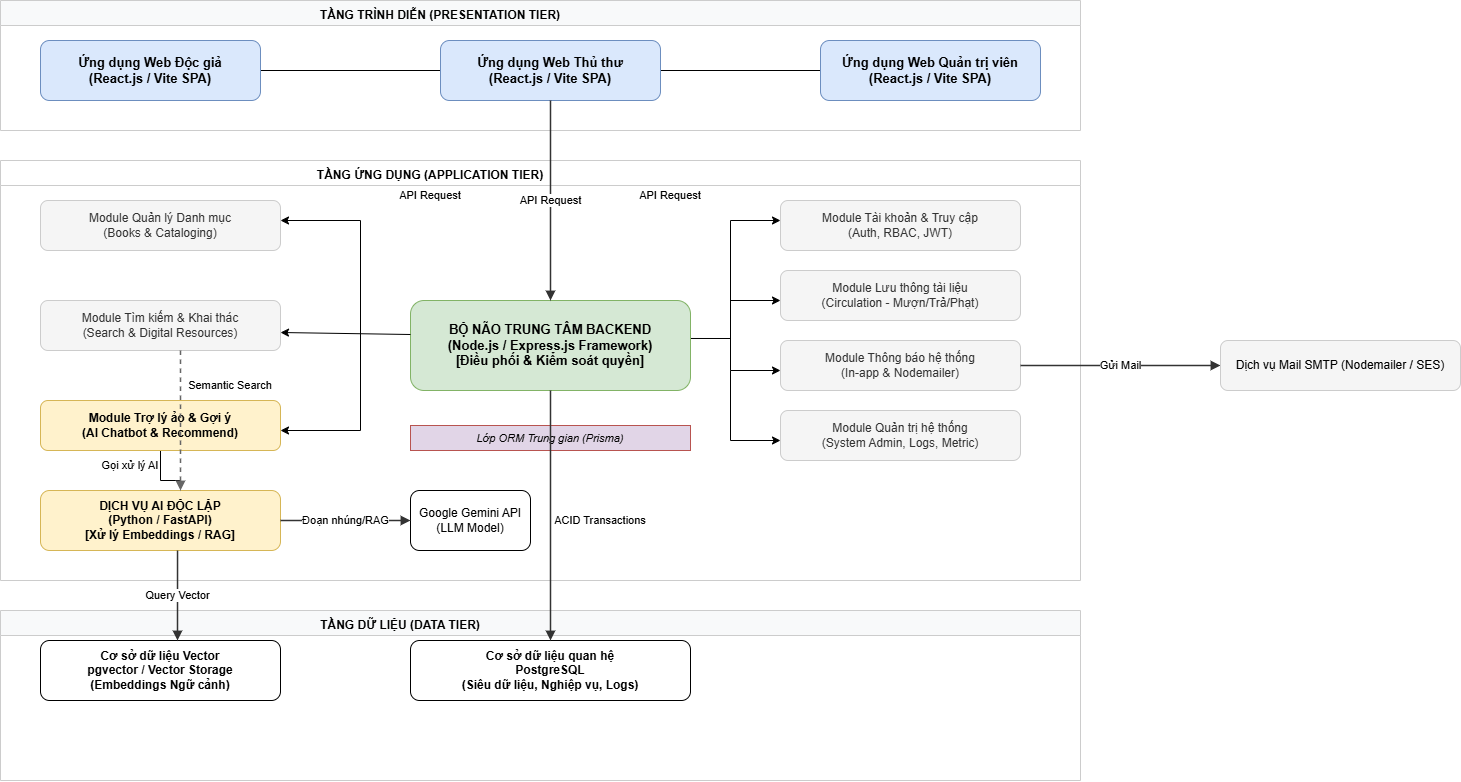
\includegraphics[width=0.6\linewidth]{Images/kientruchethong.png}
    \vspace{10pt}
    \caption{Sơ đồ kiến trúc tổng thể hệ thống Quản lý Thư viện Trực tuyến}
    \label{fig:system_architecture}
\end{figure}

Về mặt tổng thể, kiến trúc của hệ thống Quản lý Thư viện Trực tuyến được xây dựng dựa trên mô hình ba tầng tiêu chuẩn (Three-Tier Architecture), kết hợp linh hoạt với mô hình kiến trúc hướng dịch vụ (Service-Oriented) để tối ưu hóa khả năng xử lý các tác vụ Trí tuệ Nhân tạo độc lập. Ba tầng nền tảng của dự án bao gồm: Tầng Trình diễn (Presentation Tier), Tầng Ứng dụng (Application Tier) và Tầng Dữ liệu (Data Tier).

Việc áp dụng mô hình này giúp phân tách rõ ràng trách nhiệm giữa giao diện tương tác người dùng, logic xử lý nghiệp vụ thư viện và hệ quản trị cơ sở dữ liệu. Nhờ tính độc lập cao giữa các tầng, nhóm có thể dễ dàng bảo trì hoặc nâng cấp từng thành phần độc lập (chẳng hạn như tối ưu hóa thuật toán AI hoặc làm mới giao diện web) mà hoàn toàn không gây ảnh hưởng hay gián đoạn đến các quy trình cốt lõi đang vận hành ở các tầng phía dưới.

\subsubsection{Tầng Trình diễn (Presentation Tier)}
Đóng vai trò là điểm tiếp xúc trực tiếp với người sử dụng, tầng này được xây dựng dưới dạng một Ứng dụng Web Trang Đơn (Single Page Application - SPA) mạnh mẽ thông qua thư viện React.js và công cụ đóng gói Vite. Giao diện được thiết kế chuyên biệt và áp dụng cơ chế phân quyền kiểm soát nghiêm ngặt cho ba nhóm đối tượng tham gia: Độc giả (Reader), Thủ thư (Librarian) và Quản trị viên (Admin). 

Tại đây, mọi thao tác tương tác của người dùng – từ việc tìm kiếm tài liệu, gửi yêu cầu mượn sách, trò chuyện với chatbot, cho đến các thao tác quản lý chuyên sâu của thủ thư – đều được ứng dụng thu thập, xử lý bất đồng bộ và chuyển đổi thành các truy vấn RESTful API tiêu chuẩn, trước khi truyền tải xuống tầng xử lý trung tâm.

\subsubsection{Tầng Ứng dụng (Application Tier)}
Đây được xem là "bộ não" điều phối toàn bộ dự án, Tầng Ứng dụng là nơi tiếp nhận, giải quyết và thực thi các logic nghiệp vụ phức tạp của một hệ thống thư viện thông minh. Tầng này được vận hành chủ yếu bằng môi trường Node.js kết hợp framework Express.js, đồng thời tích hợp một dịch vụ độc lập viết bằng Python (FastAPI) chuyên trách các tác vụ xử lý Trí tuệ Nhân tạo hiệu năng cao. Để đảm bảo tính đóng gói và dễ mở rộng, backend được chia nhỏ thành 07 khối chức năng (Module) thực hiện ánh xạ khớp chính xác với phân hệ nghiệp vụ của hệ thống:

\begin{itemize}
    \item \textbf{Module Quản lý Tài khoản và Truy cập :} Chịu trách nhiệm bảo vệ an ninh hệ thống thông qua cơ chế phân quyền dựa trên vai trò RBAC (Role-Based Access Control) kết hợp mã hóa mật khẩu bảo mật. Hệ thống ứng dụng chuẩn Token JWT (JSON Web Token) để duy trì và xác thực các phiên làm việc một cách an toàn. Đồng thời, module này quản lý toàn bộ hồ sơ cá nhân, mã OTP xác thực và lưu vết lịch sử hoạt động cá nhân của độc giả và nhân viên.
    
    \item \textbf{Module Quản lý Danh mục sách :} Đảm nhiệm việc tổ chức và quản lý cấu trúc cây danh mục phân cấp (\texttt{Category}), lưu trữ siêu dữ liệu của các đầu sách gốc (\texttt{Book}). Phân hệ hỗ trợ thủ thư nhập liệu tự động thông qua việc tích hợp các giao tiếp API bên thứ ba (Open Library, Google Books API) để truy vấn thông tin qua mã số tiêu chuẩn ISBN.
    
    \item \textbf{Module Quản lý Lưu thông tài liệu :} Phân hệ lõi xử lý toàn bộ vòng đời mượn – trả tài liệu vật lý. Module này chịu trách nhiệm kiểm soát trạng thái lưu kho của từng bản sao (\texttt{PhysicalCopy}) qua mã vạch (Barcode), tự động hóa quy trình xếp hàng đợi đặt giữ chỗ trước (\texttt{Reservation}), tính toán điều kiện gia hạn trực tuyến, tự động áp đặt phiếu phạt tài chính (\texttt{Fine}) khi phát hiện độc giả trả sách quá hạn và điều phối lịch sử luân chuyển sách giữa các cơ sở chi nhánh vật lý.
    
    \item \textbf{Module Tìm kiếm và Khai thác tài nguyên :} Cung cấp các bộ lọc tìm kiếm nâng cao tối ưu hiệu năng truy vấn cho độc giả. Phân hệ này cũng chịu trách nhiệm số hóa thư viện thông qua việc quản lý các định dạng tài nguyên điện tử (\texttt{DigitalResource} bao gồm Ebook, Audiobook, Video), kiểm soát giới hạn số lượng độc giả truy cập và đọc tài liệu trực tuyến đồng thời nhằm đảm bảo quy định về bản quyền.
    
    \item \textbf{Module Trợ lý ảo và Gợi ý :} Hoạt động như một vi dịch vụ độc lập hiệu năng cao, tích hợp sức mạnh của các mô hình ngôn ngữ lớn (LLMs) thông qua API của Google Generative AI (Gemini). Khối chức năng này cung cấp các tính năng thông minh đột phá bao gồm: Tìm kiếm ngữ nghĩa (Semantic Search) bằng ngôn ngữ tự nhiên, tự động trích xuất nội dung để tạo tóm tắt tài liệu, chạy thuật toán dự đoán sở thích để đưa ra đề xuất sách cá nhân hóa cho từng độc giả, và vận hành một Trợ lý ảo (Chatbot) thông minh hỗ trợ giải đáp thắc mắc tự động 24/7.
    
    \item \textbf{Module Thông báo :} Đảm nhiệm vai trò tự động hóa quá trình tương tác thời gian thực với người dùng. Hệ thống sẽ tiếp nhận các sự kiện hệ thống (như sắp đến hạn trả sách, có phiếu phạt mới phát sinh, hoặc sách đặt trước đã được gom về kho sẵn sàng) để điều phối gửi thông báo qua cả hai kênh: thông báo nội bộ trong ứng dụng (In-app Notification) và thư điện tử tự động thông qua dịch vụ Nodemailer.
    
    \item \textbf{Module Quản trị hệ thống:} Cung cấp bộ công cụ tối cao dành cho người quản trị bao gồm chỉnh sửa các tham số cấu hình động hệ thống (Key-Value Config), quản lý danh sách mạng lưới chi nhánh, giám sát các chỉ số đo lường vận hành theo thời gian thực (Dashboard Metrics), kích hoạt các tiến trình sao lưu sao chụp (Backup/Snapshot) và phục hồi cơ sở dữ liệu.
\end{itemize}

Nhằm tối ưu hóa năng suất phát triển và an toàn mã nguồn, tầng Ứng dụng tích hợp công nghệ \textbf{Prisma ORM} làm lớp trung gian giao tiếp dữ liệu. Bằng cách tận dụng khả năng kiểm tra kiểu dữ liệu tĩnh nghiêm ngặt (Type-Safety) của TypeScript, Prisma giúp ngăn chặn và phát hiện sớm các lỗi cú pháp truy vấn ngay trong giai đoạn lập trình. Công cụ Prisma Migrate cũng đóng vai trò quản lý các phiên bản cấu trúc cơ sở dữ liệu (Database Schema), giúp quá trình đồng bộ hóa giữa môi trường phát triển và môi trường triển khai thực tế diễn ra an toàn, tự động.

\subsubsection{Tầng Dữ liệu (Data Tier)}
Là lớp nền tảng chịu trách nhiệm lưu trữ lâu dài, bảo mật và toàn vẹn cho toàn bộ tài nguyên thông tin của hệ thống thư viện. Tầng dữ liệu được chia làm hai thành phần lưu trữ chuyên biệt:

\begin{itemize}
    \item \textbf{Cơ sở dữ liệu quan hệ (PostgreSQL):} Đối với một hệ thống thư viện yêu cầu tính chính xác tuyệt đối trong các giao dịch tài chính và lưu thông đồng thời (ví dụ: thao tác trừ số lượng sách khả dụng trong kho và thao tác tạo phiếu mượn phải được thực hiện đồng thời), hệ quản trị \textbf{PostgreSQL} được lựa chọn nhờ hỗ trợ tính toàn vẹn giao dịch (ACID) cực kỳ nghiêm ngặt. Hệ thống sử dụng các kỹ thuật đánh chỉ mục nâng cao (Indexing) để đảm bảo tốc độ phản hồi truy vấn luôn ở mức tối ưu khi quy mô dữ liệu bản ghi tăng cao. Đặc biệt, để phục vụ công tác an ninh, mọi tác động làm thay đổi dữ liệu nhạy cảm đều được ghi vết tự động vào sổ nhật ký kiểm toán (\texttt{AuditLog}) tại tầng này.
    
    \item \textbf{Cơ sở dữ liệu Vector (Vector Database / pgvector):} Nhằm hỗ trợ phân hệ Trí tuệ Nhân tạo thực hiện kỹ thuật RAG (Retrieval-Augmented Generation) và tìm kiếm ngữ nghĩa, tầng dữ liệu tích hợp thêm cơ chế lưu trữ vector. Toàn bộ các đoạn tóm tắt sách, nội dung tài liệu và tài nguyên số sau khi được mô hình Embedding chuyển đổi thành các chuỗi vector cao chiều sẽ được lưu trữ và tính toán độ tương đồng (Cosine Similarity) trực tiếp tại đây, giúp Trợ lý ảo AI có thể truy xuất ngữ cảnh chính xác với tốc độ cao.
\end{itemize}

\subsection{Thiết kế cơ sở dữ liệu}
\subsubsection{Mô tả thực thể}

\begin{table}[H]
\centering
\begin{tabular}{|p{4cm}|p{4cm}|p{7cm}|}
\hline
\textbf{Phân loại thực thể} & \textbf{Tên thực thể} & \textbf{Ý nghĩa} \\ \hline

\multirow{5}{*}{Người dùng và phân quyền} 
& users & Lưu trữ thông tin tài khoản người dùng bao gồm bạn đọc, thủ thư và quản trị viên trong hệ thống. \\ \cline{2-3}
& roles & Quản lý vai trò và quyền hạn của người dùng như Admin, Librarian và Reader. \\ \cline{2-3}
& otp\_tokens & Lưu mã OTP phục vụ xác thực đăng nhập, đặt lại mật khẩu và bảo mật tài khoản. \\ \cline{2-3}
& notification\_settings & Lưu cấu hình nhận thông báo của người dùng qua email, SMS hoặc ứng dụng. \\ \cline{2-3}
& notifications & Quản lý các thông báo gửi đến người dùng như nhắc hạn trả sách hoặc thông báo đặt trước. \\ \hline

\multirow{5}{*}{Tài nguyên thư viện}
& books & Lưu trữ thông tin tài liệu như sách, tạp chí hoặc học liệu số trong thư viện. \\ \cline{2-3}
& categories & Quản lý danh mục và phân loại tài liệu theo chủ đề hoặc lĩnh vực. \\ \cline{2-3}
& physical\_copies & Quản lý từng bản sao vật lý của tài liệu cùng trạng thái sử dụng và vị trí lưu trữ. \\ \cline{2-3}
& digital\_resources & Lưu thông tin tài nguyên số như Ebook hoặc tài liệu PDF phục vụ truy cập trực tuyến. \\ \cline{2-3}
& digital\_access\_logs & Ghi nhận lịch sử truy cập tài nguyên số của người dùng nhằm theo dõi và thống kê sử dụng. \\ \hline

\multirow{5}{*}{Nghiệp vụ thư viện}
& borrow\_records & Quản lý quá trình mượn và trả tài liệu của người dùng. \\ \cline{2-3}
& reservations & Quản lý chức năng đặt trước tài liệu khi tài liệu chưa sẵn sàng cho mượn. \\ \cline{2-3}
& fines & Quản lý các khoản phí phạt phát sinh do trả trễ hoặc vi phạm quy định thư viện. \\ \cline{2-3}
& branches & Lưu thông tin các chi nhánh thư viện và hỗ trợ quản lý tài nguyên theo từng cơ sở. \\ \cline{2-3}
& branch\_transfers & Quản lý việc điều chuyển bản sao tài liệu giữa các chi nhánh thư viện. \\ \hline

\multirow{2}{*}{Tương tác và đánh giá}
& reviews & Lưu đánh giá, nhận xét và xếp hạng tài liệu từ người dùng nhằm hỗ trợ gợi ý và cải thiện trải nghiệm. \\ \cline{2-3}
& chat\_history & Lưu lịch sử trao đổi giữa người dùng và chatbot/trợ lý ảo AI của hệ thống. \\ \hline

\multirow{2}{*}{Hệ thống và quản trị}
& audit\_logs & Ghi nhận lịch sử hoạt động và thao tác của người dùng để phục vụ kiểm toán và bảo mật hệ thống. \\ \cline{2-3}
& system\_configs & Lưu các tham số và cấu hình hoạt động chung của hệ thống thư viện. \\ \hline

\end{tabular}
\caption{Danh sách các thực thể trong hệ thống}
\label{tab:entity-description}
\end{table}

\subsubsection{Sơ đồ thực thể liên kết (EERD)}

\begin{figure}[H]
    \centering
    \includegraphics[width=\linewidth]{Images/ERD.png}
    \vspace{10pt}
    \caption{Sơ đồ EERD Hệ thống Quản lý thư viện trực tuyến}
    \label{fig:erd_account}
\end{figure}



Dựa trên sơ đồ thực thể liên kết (ERD) , luồng vận hành của hệ thống Quản lý thư viện trực tuyến được phân định rõ ràng thành các phân hệ nghiệp vụ chuyên biệt tương ứng với 3 vai trò người dùng cốt lõi:

\paragraph{Bạn đọc}
Đây là đối tượng sử dụng cuối (End-user), tương tác với hệ thống nhằm khai thác các tài nguyên học thuật trực tuyến và trực tiếp. Các nghiệp vụ cụ thể bao gồm:
\begin{itemize}
    \item \textbf{Quản lý tài khoản và Bảo mật:} Thực hiện các quy trình xác thực đa yếu tố bằng mã bảo mật dùng một lần thông qua bảng \texttt{otp\_tokens}; chủ động cá nhân hóa các kênh nhận diện thông báo hệ thống (Email, SMS, In-app) tại bảng \texttt{notification\_settings}.
    \item \textbf{Khai thác tài nguyên số:} Tìm kiếm, phân loại tài liệu học tập theo danh mục chủ đề (\texttt{categories}). Bạn đọc có quyền truy cập, đọc trực tuyến hoặc tải xuống tài liệu điện tử (\texttt{digital\_resources}), mọi hành vi khai thác này đều được ghi nhận tự động vào bảng \texttt{digital\_access\_logs}.
    \item \textbf{Mượn - Trả sách vật lý:} Tạo lập yêu cầu và theo dõi vòng đời của quá trình mượn, gia hạn sách vật lý tại bảng \texttt{borrow\_records} liên kết với từng bản sao cụ thể (\texttt{physical\_copies}).
    \item \textbf{Xử lý hàng đợi đặt trước:} Khi một cuốn sách đã hết bản sao sẵn sàng, bạn đọc có thể thực hiện đăng ký đặt giữ chỗ trước (\texttt{reservations}) và được xếp thứ tự hàng đợi tự động qua thuộc tính \texttt{queuePosition}.
    \item \textbf{Tương tác phản hồi:} Ghi nhận trải nghiệm đọc thông qua việc chấm điểm và viết nhận xét về tài liệu (\texttt{reviews}); trao đổi thông tin trực tuyến với Trợ lý ảo AI nhằm giải đáp thắc mắc, thông tin hội thoại được lưu giữ trong bảng \texttt{chat\_history}. Theo dõi và thực hiện thanh toán các khoản phí phạt (\texttt{fines}) nếu phát sinh tình trạng quá hạn.
\end{itemize}

\paragraph{Thủ thư}
Thủ thư đóng vai trò là người điều hành, kiểm soát và thực hiện trực tiếp các nghiệp vụ quản lý kho bãi, tương tác vật lý với bạn đọc tại các cơ sở. Các nghiệp vụ cụ thể bao gồm:
\begin{itemize}
    \item \textbf{Quản trị kho sách vật lý:} Cập nhật, chỉnh sửa danh mục sách (\texttt{books}), quản lý số lượng, trạng thái (\texttt{status}), tình trạng hao mòn (\texttt{condition}) cũng như vị trí xếp giá cụ thể (\texttt{location}) của từng bản sao vật lý (\texttt{physical\_copies}) thuộc chi nhánh phụ trách.
    \item \textbf{Xử lý trực tiếp quy trình Mượn - Trả:} Tiếp nhận yêu cầu từ bạn đọc, thực hiện kiểm tra mã vạch (\texttt{barcode}) của sách và mã bạn đọc (\texttt{readerCode}), trực tiếp cập nhật thông tin và phê duyệt các bản ghi \texttt{borrow\_records}.
    \item \textbf{Điều phối hàng đợi và Giữ sách:} Theo dõi danh sách bạn đọc đăng ký giữ chỗ trước tại bảng \texttt{reservations}, thực hiện chuyển trạng thái khi sách được hoàn trả và gửi thông báo tự động cho bạn đọc có lượt kế tiếp.
    \item \textbf{Điều chuyển tài nguyên liên chi nhánh:} Tạo lập, phê duyệt và cập nhật tiến độ vận chuyển, bàn giao các bản sao sách giữa các chi nhánh thư viện khác nhau thông qua bảng \texttt{branch\_transfers}.
    \item \textbf{Quản lý phạt và Miễn giảm phí:} Phát hiện, ghi nhận các trường hợp vi phạm quy định thư viện, áp mức phạt tự động hoặc thủ công vào bảng \texttt{fines}. Thủ thư có thẩm quyền thực hiện xét duyệt miễn giảm hoặc xóa phạt (\texttt{waivedById}) đi kèm với lý do cụ thể (\texttt{waivedReason}).
\end{itemize}

\paragraph{Quản trị viên}
Quản trị viên giữ vai trò cấu hình, giám sát tối cao toàn bộ hệ thống kỹ thuật và đảm bảo tính an toàn dữ liệu. Các nghiệp vụ cụ thể bao gồm:
\begin{itemize}
    \item \textbf{Quản lý người dùng và Phân quyền chuyên sâu:} Khởi tạo, khóa/mở khóa tài khoản (\texttt{users}), kiểm soát số lần đăng nhập sai (\texttt{failedLoginCount}) và thời gian khóa tài khoản tạm thời (\texttt{lockedUntil}). Phân định quyền hạn hệ thống một cách nghiêm ngặt thông qua liên kết cấu trúc vai trò (\texttt{roles}).
    \item \textbf{Quản trị hạ tầng mạng lưới:} Khởi tạo, kích hoạt hoặc tạm dừng hoạt động của các cơ sở, chi nhánh thư viện (\texttt{branches}), đồng thời chỉ định nhân sự chịu trách nhiệm quản lý chi nhánh (\texttt{managerId}).
    \item \textbf{Cấu hình tham số toàn cục:} Thiết lập các quy định, chính sách ngầm định của toàn bộ thư viện thông qua bảng \texttt{system\_configs} (ví dụ: đơn giá phạt/ngày, giới hạn số ngày mượn tối đa, dung lượng tệp tin số tối đa).
    \item \textbf{Kiểm toán và Bảo mật hệ thống:} Giám sát toàn bộ các hành vi mang tính thay đổi dữ liệu lớn hoặc can thiệp sâu của thủ thư và người dùng thông qua nhật ký kiểm toán hệ thống (\texttt{audit\_logs}) để kịp thời phát hiện lỗi hệ thống hoặc lỗ hổng bảo mật.
\end{itemize}



\subsubsection{Lược đồ cơ sở dữ liệu (Database)}
\begin{figure}[H]
    \centering
    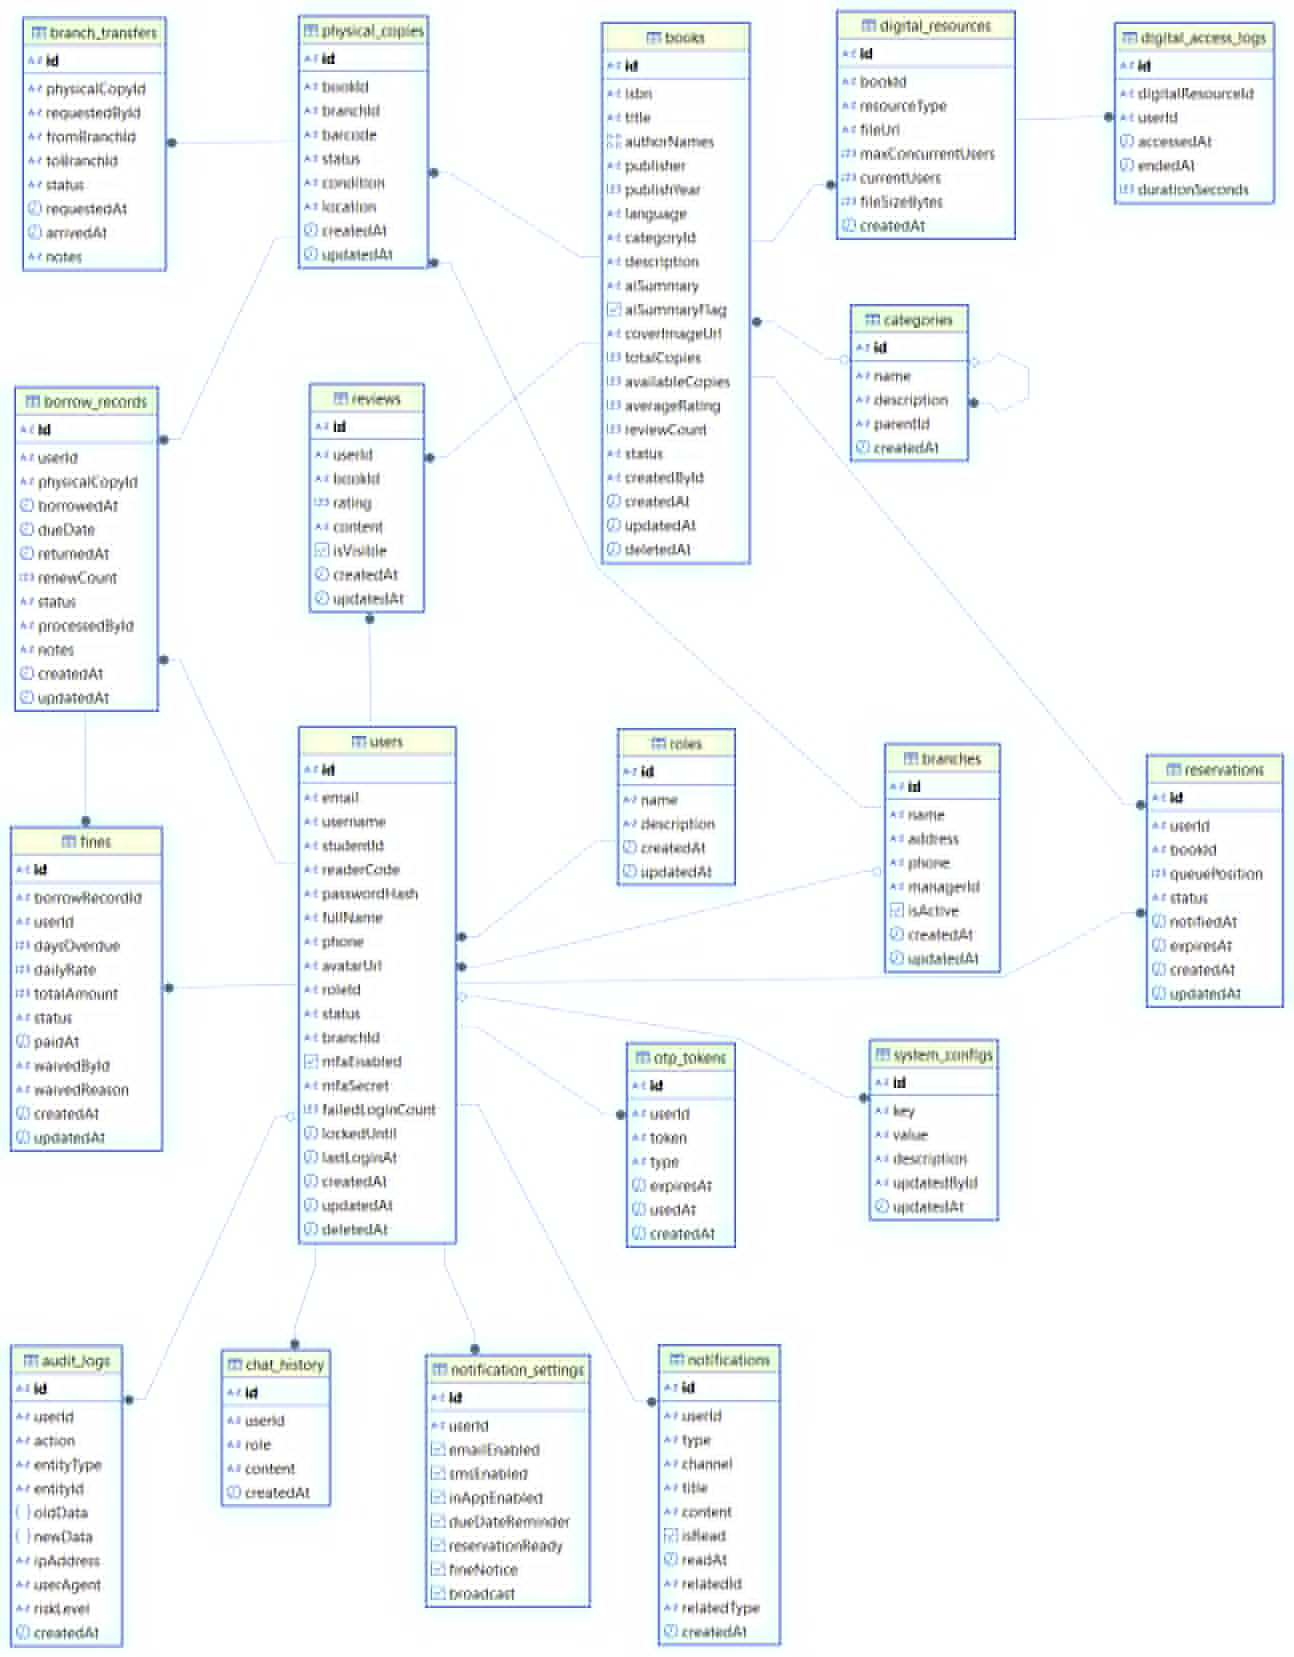
\includegraphics[width=0.6\linewidth]{Images/db.jpg}
    \vspace{10pt}
    \caption{Lược đồ cơ sở dữ liệu Hệ thống Quản lý thư viện trực tuyến}
    \label{fig:database_account}
\end{figure}
Lược đồ trên là cơ sở dữ liệu của hệ thống Quản lý thư viện trực tuyến khi được hiện thực trên cơ sở dữ liệu PostgreSQL.



Để thực hiện việc quản lý đơn giản người dùng của hệ thống, ở đây nhóm chỉ thiết kế một bảng duy nhất là \texttt{users} để lưu trữ tập trung thông tin tài khoản. Để có thể phân biệt và phân quyền chính xác người dùng thuộc vai trò nào trong 3 nhóm Reader, Librarian, hay Admin, nhóm sử dụng cơ chế liên kết với bảng danh mục \texttt{roles} qua khóa ngoại \texttt{roleId}. Đồng thời, các thuộc tính phụ tích hợp trong bảng \texttt{users} bao gồm \texttt{status} (kiểm tra trạng thái hoạt động), \texttt{failedLoginCount} (đếm số lần đăng nhập sai) và \texttt{lockedUntil} (thời gian khóa tài khoản tạm thời) được áp dụng nhằm kiểm tra, kiểm soát chặt chẽ trạng thái an ninh đăng nhập của người dùng,quản lý vai trò cũng như quyền hạn của người dùng.

Với các bảng còn lại nhóm thực hiện mapping chính xác theo sơ đồ thực thể liên kết và bảng mô tả thực thể  đã được trình bày bên trên.







\subsection{Sơ đồ lớp (Class Diagram)}

\subsubsection{Quản lý tài khoản và truy cập}

\begin{figure}[H]
    \centering
    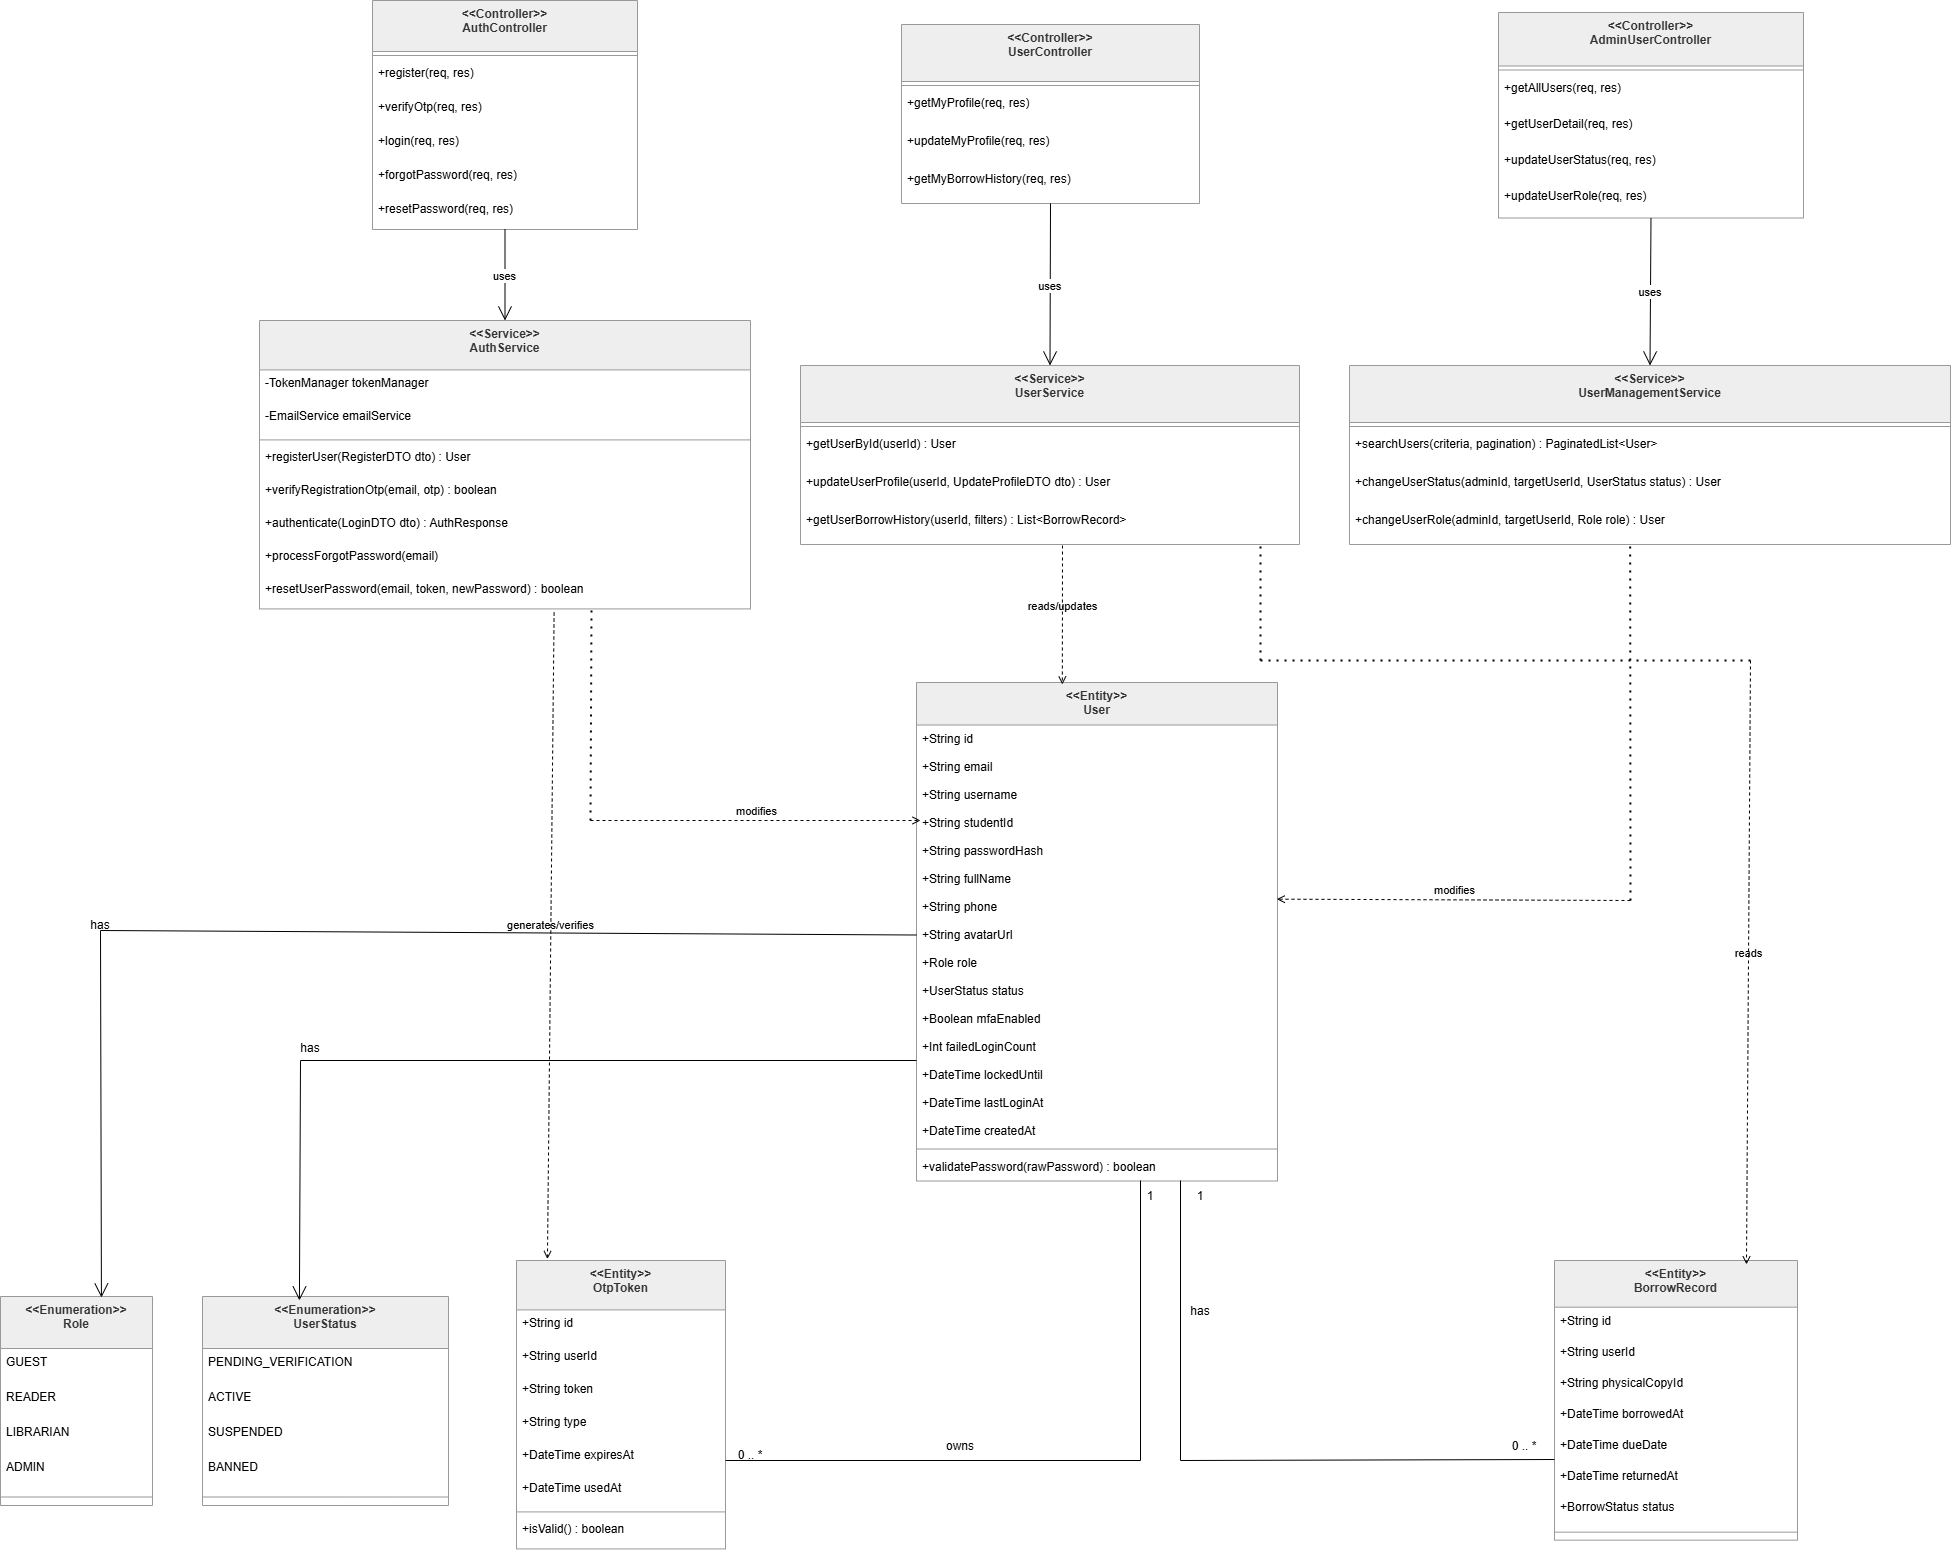
\includegraphics[width=0.6\linewidth]{Images/quanlytruycapvataikhoan.png}
    \vspace{10pt}
    \caption{Sơ đồ lớp Quản lý tài khoản và truy cập}
    \label{fig:class_account}
\end{figure}

Dựa vào các nghiệp vụ và lược đồ thực thể mối liên hệ mở rộng, sơ đồ lớp được thiết kế nhằm để thể hiện việc mô hình hóa các đối tượng trong phân hệ \textbf{Quản lý tài khoản và truy cập} bao gồm các thuộc tính và các phương thức xử lý chính.

Đầu tiên, hệ thống tập trung xoay quanh một thực thể trung tâm là \texttt{User}. Lớp \texttt{User} này chứa toàn bộ các thuộc tính định danh cơ bản của một người dùng như \texttt{id}, \texttt{email}, \texttt{username}, \texttt{fullName}, \texttt{phone}, \texttt{avatarUrl}, \texttt{studentId}, cùng các thuộc tính phục vụ bảo mật nâng cao và nhật ký hệ thống như \texttt{passwordHash}, \texttt{mfaEnabled}, \texttt{failedLoginCount}, \texttt{lockedUntil}, \texttt{lastLoginAt}, và \texttt{createdAt}. Đặc biệt, lớp \texttt{User} này có phương thức xử lý chính là \texttt{validatePassword(rawPassword)} dùng để kiểm tra tính hợp lệ của mật khẩu khi thực hiện các tác vụ xác thực. 

Để quản lý vai trò và trạng thái của người dùng, lớp \texttt{User} có mối liên hệ association với hai danh mục là \texttt{Role} và \texttt{UserStatus}. Trong đó, danh mục \texttt{Role} thể hiện việc phân quyền trong hệ thống với 4 cấp độ bao gồm \texttt{GUEST}, \texttt{READER}, \texttt{LIBRARIAN}, và \texttt{ADMIN}. Còn danh mục \texttt{UserStatus} thể hiện vòng đời hoạt động của tài khoản qua các trạng thái \texttt{PENDING\_VERIFICATION}, \texttt{ACTIVE}, \texttt{SUSPENDED}, và \texttt{BANNED}.

Theo sơ đồ lớp, ta thấy lớp \texttt{User} có mối liên hệ association với lớp \texttt{OtpToken} với quan hệ $1 - 0..*$, thể hiện việc một \texttt{User} tại một thời điểm có thể sở hữu nhiều hoặc không sở hữu mã OTP nào, dùng cho các mục đích xác thực an toàn. Lớp \texttt{OtpToken} này có phương thức xử lý chính là \texttt{isValid()} để tự kiểm tra thời gian hết hạn và trạng thái sử dụng của mã. Bên cạnh đó, lớp \texttt{User} còn có mối liên hệ association với lớp \texttt{BorrowRecord} với quan hệ $1 - 0..*$, thể hiện việc một người dùng có thể sở hữu nhiều bản ghi lịch sử mượn sách trong hệ thống thư viện.

Về mặt kiến trúc vận hành logic nghiệp vụ, sơ đồ lớp được phân tách rõ ràng thành các tầng \texttt{Controller} và \texttt{Service} tương ứng để xử lý các yêu cầu từ người dùng:

Đối với luồng nghiệp vụ Xác thực và Bảo mật, lớp \texttt{AuthController} sử dụng lớp \texttt{AuthService} để hiện thực hóa các phương thức xử lý chính bao gồm đăng ký tài khoản (\texttt{registerUser}), xác thực mã OTP (\texttt{verifyRegistrationOtp}), đăng nhập hệ thống (\texttt{authenticate}), xử lý quên mật khẩu (\texttt{processForgotPassword}), và đặt lại mật khẩu mới (\texttt{resetPasswordUser}). Lớp \texttt{AuthService} này sẽ có mối quan hệ phụ thuộc để tiến hành tạo hoặc xác thực dữ liệu trên lớp \texttt{OtpToken}, đồng thời thực hiện chỉnh sửa dữ liệu trên lớp \texttt{User}.

Đối với luồng nghiệp vụ cá nhân của người dùng, lớp \texttt{UserController} sử dụng lớp \texttt{UserService} để thực hiện các hành động xem thông tin cá nhân (\texttt{getUserById}), cập nhật hồ sơ (\texttt{updateUserProfile}), và đọc danh sách lịch sử mượn sách (\texttt{getUserBorrowHistory}). Lớp \texttt{UserService} này có mối liên hệ đọc và cập nhật trực tiếp với thực thể \texttt{User}, cũng như đọc dữ liệu từ thực thể \texttt{BorrowRecord}.

Đến với việc quản lý vận hành của người quản trị, sơ đồ lớp cho ta thấy lớp \texttt{AdminUserController} sẽ sử dụng lớp \texttt{UserManagementService} để thực hiện các chức năng quản trị diện rộng. Các phương thức xử lý chính tại đây bao gồm tìm kiếm người dùng theo tiêu chí kết hợp phân trang (\texttt{searchUsers}), xem chi tiết tài khoản (\texttt{getUserDetail}), thay đổi trạng thái hoạt động của tài khoản (\texttt{changeUserStatus}), và thực hiện phân lại vai trò cho người dùng (\texttt{changeUserRole}). Lớp \texttt{UserManagementService} này thể hiện quyền hạn tối cao của người Admin khi có mối liên hệ đọc và chỉnh sửa trực tiếp lên thực thể \texttt{User}, đồng thời có mối liên hệ đọc thông tin từ thực thể \texttt{BorrowRecord} để phục vụ công tác kiểm tra, giám sát hệ thống.

\subsubsection{Quản lý danh mục sách}

\begin{figure}[H]
    \centering
    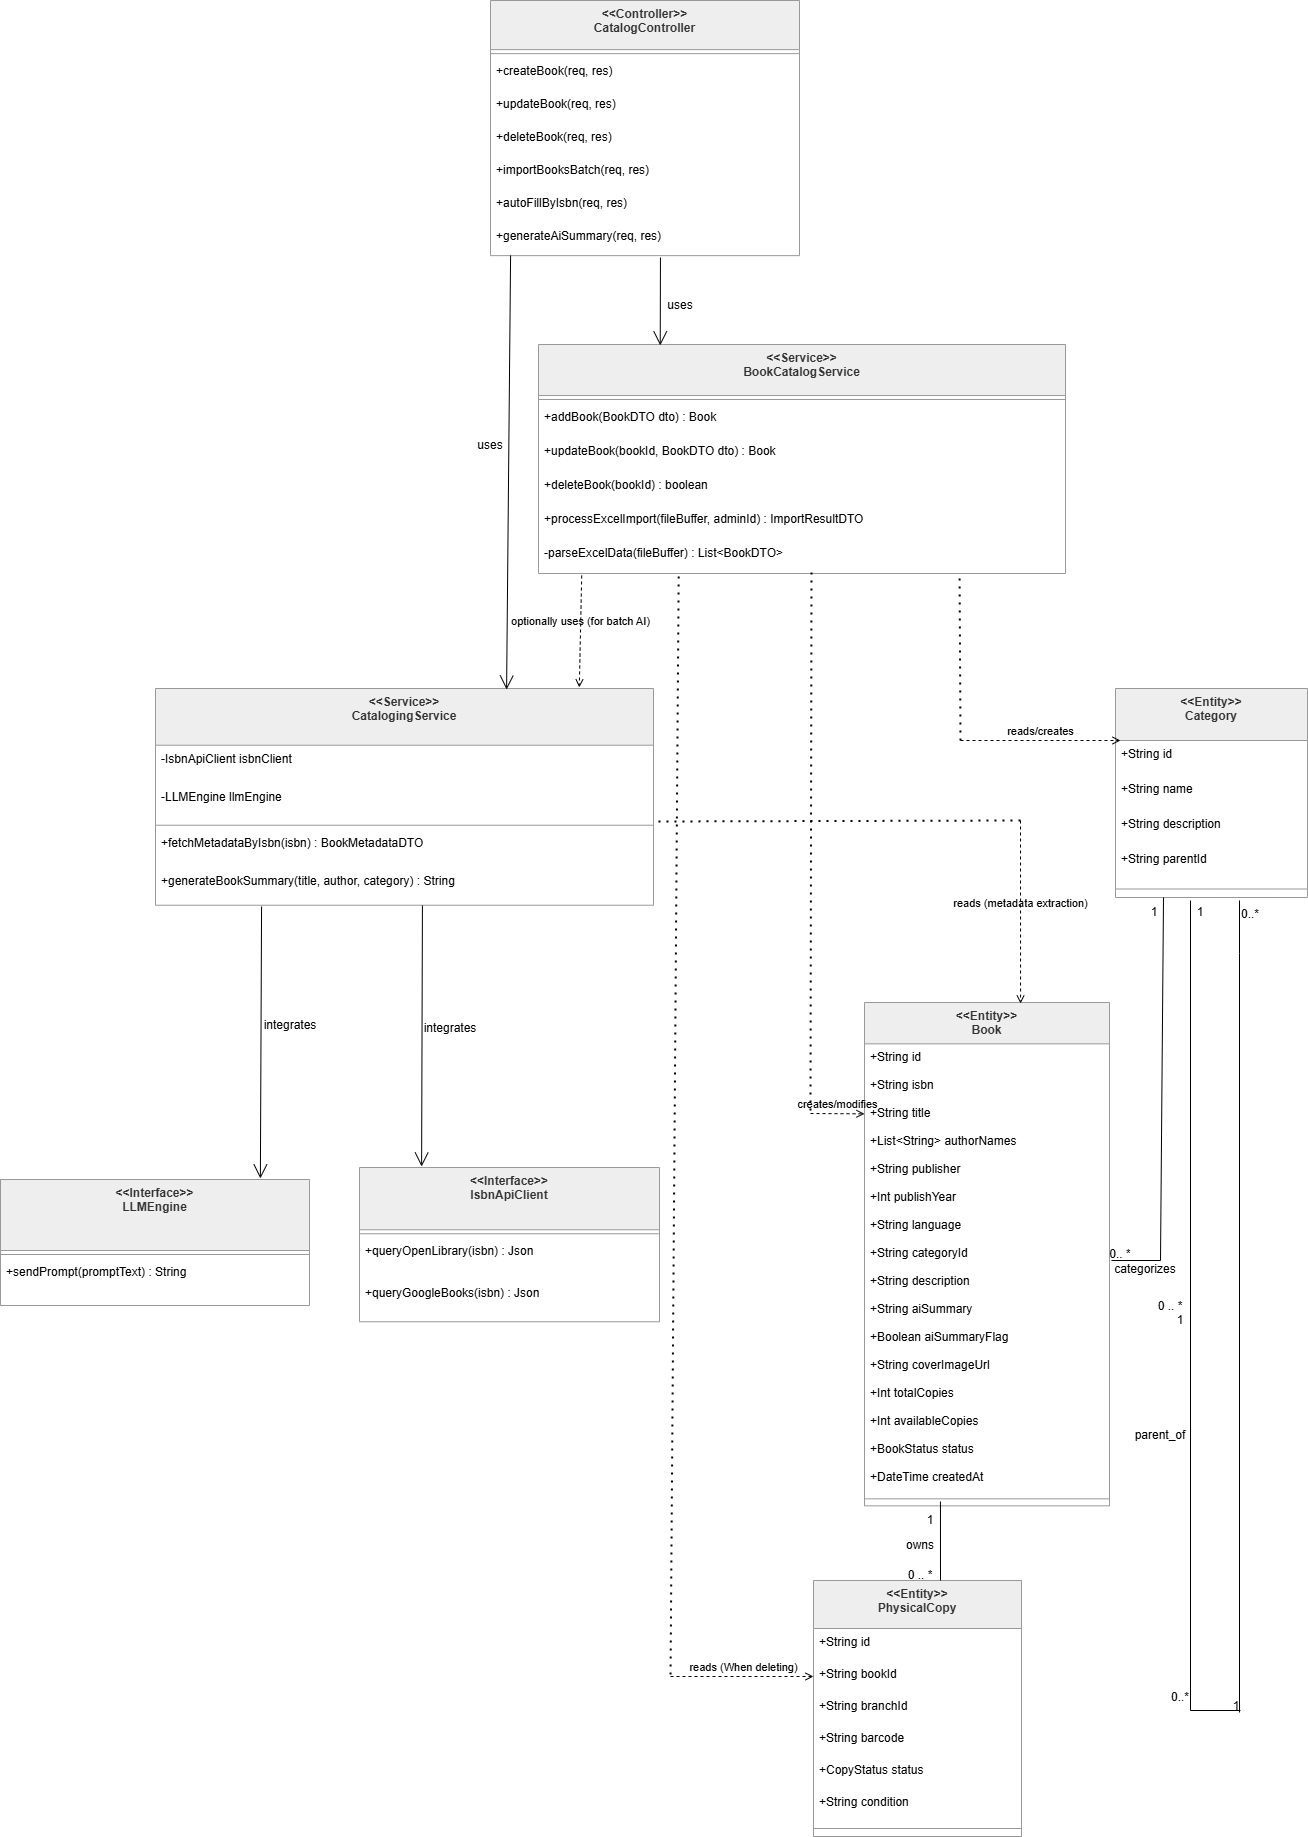
\includegraphics[width=0.6\linewidth]{Images/quanlydanhmuc.png}
    \vspace{10pt}
    \caption{Sơ đồ lớp Quản lý danh mục sách}
    \label{fig:class_catalog}
\end{figure}

Sơ đồ lớp phân hệ này được thiết kế nhằm để thể hiện việc mô hình hóa các đối tượng trong phân hệ \textbf{Quản lý danh mục sách} bao gồm các thuộc tính và các phương thức xử lý chính.

Đầu tiên, cấu trúc dữ liệu cốt lõi của phân hệ này tập trung vào ba thực thể chính có mối quan hệ ràng buộc chặt chẽ với nhau là \texttt{Category}, \texttt{Book}, và \texttt{PhysicalCopy}. Đối với thực thể \texttt{Category} (Danh mục), lớp này chứa các thông tin \texttt{id}, \texttt{name}, \texttt{description}, và \texttt{parentId}. Giữa \texttt{Category} và chính nó có mối quan hệ association hồi quy với quan hệ $1 - 0..*$ thông qua thuộc tính \texttt{parentId}, thể hiện cho việc một danh mục cha có thể chứa nhiều danh mục con bên trong, tạo thành một cấu trúc cây thư mục hoàn chỉnh. Giữa \texttt{Category} và thực thể \texttt{Book} có mối liên hệ association với tỷ lệ $1 - 0..*$, cho ta thấy một danh mục sẽ bao gồm nhiều cuốn sách thuộc về danh mục đó. 

Đến với thực thể \texttt{Book}, lớp này chứa rất nhiều thuộc tính chi tiết như \texttt{id}, \texttt{isbn}, \texttt{title}, \texttt{authorNames}, \texttt{publisher}, \texttt{publishYear}, \texttt{language}, \texttt{coverImageUrl}, \texttt{totalCopies}, \texttt{availableCopies}, và các thuộc tính thông minh như \texttt{aiSummary}, \texttt{aiSummaryFlag}. Mỗi một đầu sách (\texttt{Book}) sẽ có mối quan hệ association sâu sắc với bản sao vật lý của nó là lớp \texttt{PhysicalCopy} theo tỷ lệ $1 - 0..*$. Điều này thể hiện một đầu sách trong thư viện có thể có nhiều bản sao thực tế nằm ở các kệ hoặc chi nhánh khác nhau. Lớp \texttt{PhysicalCopy} sở hữu các thông tin quản lý lưu kho cụ thể như \texttt{id}, \texttt{bookId}, \texttt{branchId}, \texttt{barcode}, trạng thái sách \texttt{CopyStatus status}, và tình trạng vật lý \texttt{condition}.

Về mặt kiến trúc và luồng điều hướng nghiệp vụ, phân hệ được phân rã thành các thành phần controller và service xử lý như sau:

Lớp \texttt{CatalogController} giữ vai trò tiếp nhận các yêu cầu điều khiển từ người vận hành hệ thống, sau đó chuyển giao xử lý xuống lớp \texttt{BookCatalogService}. Tại lớp \texttt{BookCatalogService}, các phương thức xử lý nghiệp vụ chính được hiện thực bao gồm: thêm sách mới (\texttt{addBook}), cập nhật thông tin sách (\texttt{updateBook}), xóa sách (\texttt{deleteBook}), tự động điền thông tin qua mã ISBN (\texttt{autoFillByIsbn}), và kích hoạt tính năng tạo tóm tắt nội dung bằng AI (\texttt{generateAiSummary}). Ngoài ra, dịch vụ này còn hỗ trợ nhập liệu sách hàng loạt từ file Excel thông qua hàm \texttt{processExcelImport(fileBuffer, adminId)} để chuyển đổi thành cấu trúc \texttt{ImportResultDTO}. Lớp \texttt{BookCatalogService} có mối quan hệ trực tiếp để tạo mới hoặc cập nhật dữ liệu trên hai thực thể là \texttt{Category} và \texttt{Book}, đồng thời nó có cơ chế kiểm tra ràng buộc bằng cách đọc dữ liệu từ lớp \texttt{PhysicalCopy} khi thực hiện hành động xóa sách.

Một điểm nổi bật trong thiết kế của phân hệ này là mối quan hệ phụ thuộc bổ trợ giữa \texttt{BookCatalogService} và lớp nghiệp vụ thông minh \texttt{CatalogingService}. Lớp \texttt{CatalogingService} đóng vai trò là một dịch vụ trung gian chuyên biệt để xử lý dữ liệu ngoại vi và AI. Lớp này tích hợp hai giao tiếp (interface) hệ thống là \texttt{IsbnApiClient} (chứa phương thức truy vấn API từ các nguồn dữ liệu mở \texttt{queryOpenLibrary} và \texttt{queryGoogleBooks}) dùng để tự động lấy siêu dữ liệu sách (\texttt{fetchMetadataByIsbn}), kết hợp cùng giao tiếp \texttt{LLMEngine} nhằm tự động hóa việc trích xuất và sinh ra các đoạn tóm tắt nội dung ngắn gọn cho sách (\texttt{generateBookSummary}). Sau khi xử lý xong, \texttt{CatalogingService} sẽ tiến hành ghi đè các trường dữ liệu meta thu được vào thẳng thực thể \texttt{Book}.

\subsubsection{Quản lý lưu thông tài liệu}

\begin{figure}[H]
    \centering
    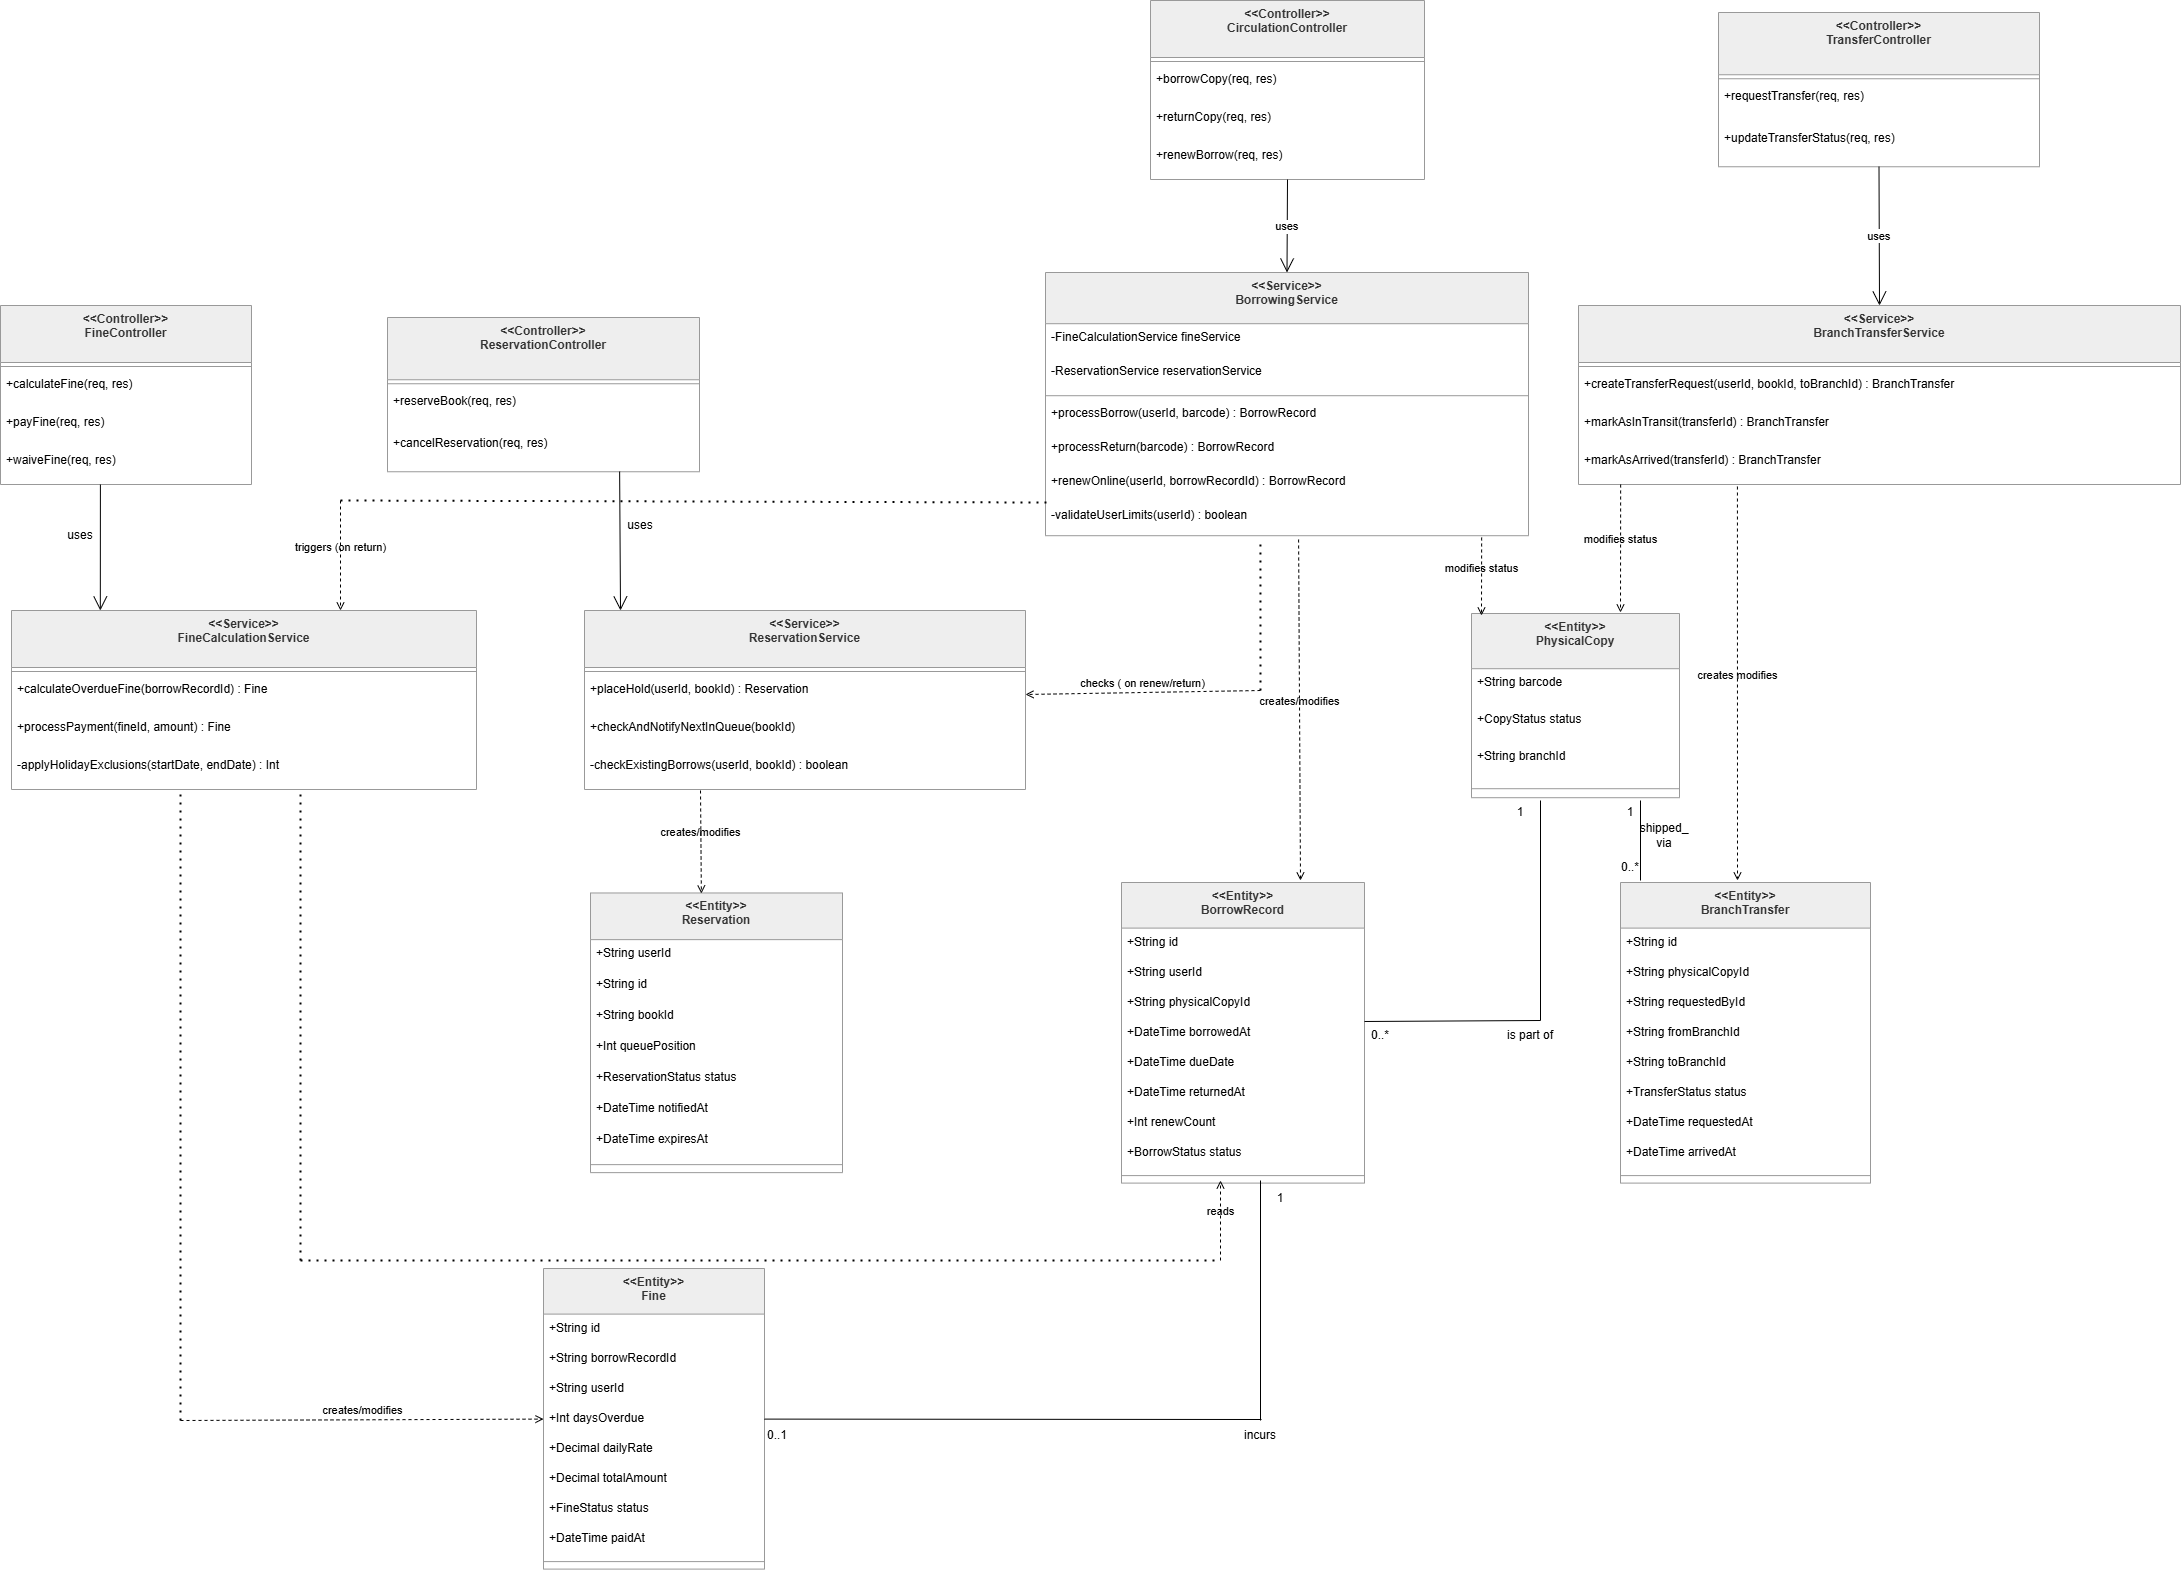
\includegraphics[width=0.6\linewidth]{Images/quanlyluuthong.png}
    \vspace{10pt}
    \caption{Sơ đồ lớp Quản lý lưu thông tài liệu}
    \label{fig:class_circulation}
\end{figure}

Sơ đồ lớp phân hệ này được thiết kế nhằm để thể hiện việc mô hình hóa các đối tượng trong phân hệ \textbf{Quản lý lưu thông tài liệu} bao gồm các thuộc tính và các phương thức xử lý chính.

Đầu tiên, trung tâm của phân hệ lưu thông là thực thể \texttt{BorrowRecord} (Nhật ký mượn sách). Lớp này lưu trữ các thuộc tính trạng thái và thời gian cốt lõi như \texttt{id}, \texttt{userId}, \texttt{physicalCopyId}, \texttt{borrowedAt}, \texttt{dueDate}, \texttt{returnedAt}, \texttt{renewCount}, và trạng thái \texttt{BorrowStatus status}. Để quản lý chi tiết đối tượng mượn, thực thể \texttt{PhysicalCopy} (Bản sao vật lý) có mối quan hệ association với \texttt{BorrowRecord} theo tỷ lệ $1 - 0..*$, thể hiện một bản sao vật lý cụ thể tại một thời điểm chỉ nằm trong một lượt mượn nhưng có thể thuộc về nhiều lượt mượn khác nhau theo thời gian. 

Bên cạnh đó, hệ thống tích hợp hai thực thể phụ thuộc để giải quyết các nghiệp vụ phát sinh xung quanh lượt mượn. Đầu tiên là thực thể \texttt{Reservation} (Đặt chỗ trước) chứa các trường \texttt{userId}, \texttt{id}, \texttt{bookId}, \texttt{queuePosition}, \texttt{ReservationStatus status}, cùng mốc thời gian thông báo và hết hạn. Thực thể thứ hai là \texttt{Fine} (Phiếu phạt quá hạn) có mối quan hệ association $1 - 0..1$ với \texttt{BorrowRecord}, nghĩa là một lượt mượn sách nếu trả trễ sẽ chỉ phát sinh tối đa một phiếu phạt tương ứng. Lớp \texttt{Fine} quản lý các thông tin tài chính gồm \texttt{id}, \texttt{borrowRecordId}, \texttt{userId}, số ngày trễ (\texttt{daysOverdue}), đơn giá phạt (\texttt{dailyRate}), tổng tiền (\texttt{totalAmount}), trạng thái thanh toán \texttt{FineStatus status}, và ngày trả tiền (\texttt{paidAt}). Ngoài ra, đối với việc vận chuyển sách giữa các cơ sở, thực thể \texttt{BranchTransfer} được thiết kế kết nối với \texttt{PhysicalCopy} qua quan hệ $1 - 0..*$, nhằm theo dõi các thông tin điều phối như \texttt{fromBranchId}, \texttt{toBranchId}, trạng thái vận chuyển, ngày yêu cầu và ngày đến nơi.

Về mặt cấu trúc điều hướng logic nghiệp vụ, phân hệ được phân rã thành các luồng xử lý riêng biệt thông qua các tầng Controller và Service chuyên trách:

Đối với luồng nghiệp vụ Mượn trả chính, lớp \texttt{CirculationController} sử dụng lớp \texttt{BorrowingService} để thực thi các hàm xử lý bao gồm: mượn sách (\texttt{processBorrow}), trả sách (\texttt{processReturn}), và gia hạn trực tuyến (\texttt{renewOnline}). Để đảm bảo các quy định của thư viện, lớp \texttt{BorrowingService} sẽ gọi hàm nội bộ \texttt{validateUserLimits(userId)} nhằm kiểm tra giới hạn thẻ mượn của độc giả. Đồng thời, khi thực hiện gia hạn hoặc trả sách, dịch vụ này có mối quan hệ phụ thuộc để kiểm tra chéo dữ liệu trạng thái hàng đợi với lớp \texttt{ReservationService}, sau đó tiến hành cập nhật trực tiếp lên hai thực thể \texttt{BorrowRecord} và \texttt{PhysicalCopy}.

Đối với luồng nghiệp vụ Đặt chỗ trước, lớp \texttt{ReservationController} sử dụng lớp \texttt{ReservationService} để xử lý các hành động đăng ký giữ chỗ (\texttt{placeHold}) và hủy đặt chỗ (\texttt{cancelReservation}). Lớp dịch vụ này giữ vai trò tính toán thứ tự ưu tiên thông qua hàm \texttt{checkAndNotifyNextInQueue(bookId)} trước khi tiến hành ghi dữ liệu vào thực thể \texttt{Reservation}.

Đối với luồng nghiệp vụ Tính toán và Xử lý phạt, lớp \texttt{FineController} phối hợp cùng lớp \texttt{FineCalculationService} để thực hiện tính toán tiền phạt trễ hạn (\texttt{calculateOverdueFine}), xử lý thanh toán tiền phạt (\texttt{processPayment}), và xem xét miễn giảm phạt (\texttt{applyHolidayExclusions}). Lớp dịch vụ này hoạt động dựa trên cơ chế kích hoạt tự động từ hệ thống mượn trả khi phát hiện sách trả trễ hạn, từ đó tạo mới hoặc chỉnh sửa dữ liệu trên thực thể \texttt{Fine}.

Cuối cùng, đối với luồng nghiệp vụ Luân chuyển sách giữa các chi nhánh, lớp \texttt{TransferController} sử dụng lớp \texttt{BranchTransferService} nhằm xử lý các yêu cầu điều phối sách (\texttt{createTransferRequest}), đánh dấu trạng thái đang vận chuyển (\texttt{markInTransit}), và xác nhận sách đã đến nơi (\texttt{markAsArrived}). Lớp này có mối quan hệ chỉnh sửa trực tiếp thuộc tính vị trí kho trên thực thể \texttt{PhysicalCopy} và lưu vết lịch sử vận chuyển vào thực thể \texttt{BranchTransfer}.

\subsubsection{Tìm kiếm và khai thác tài nguyên}

\begin{figure}[H]
    \centering
    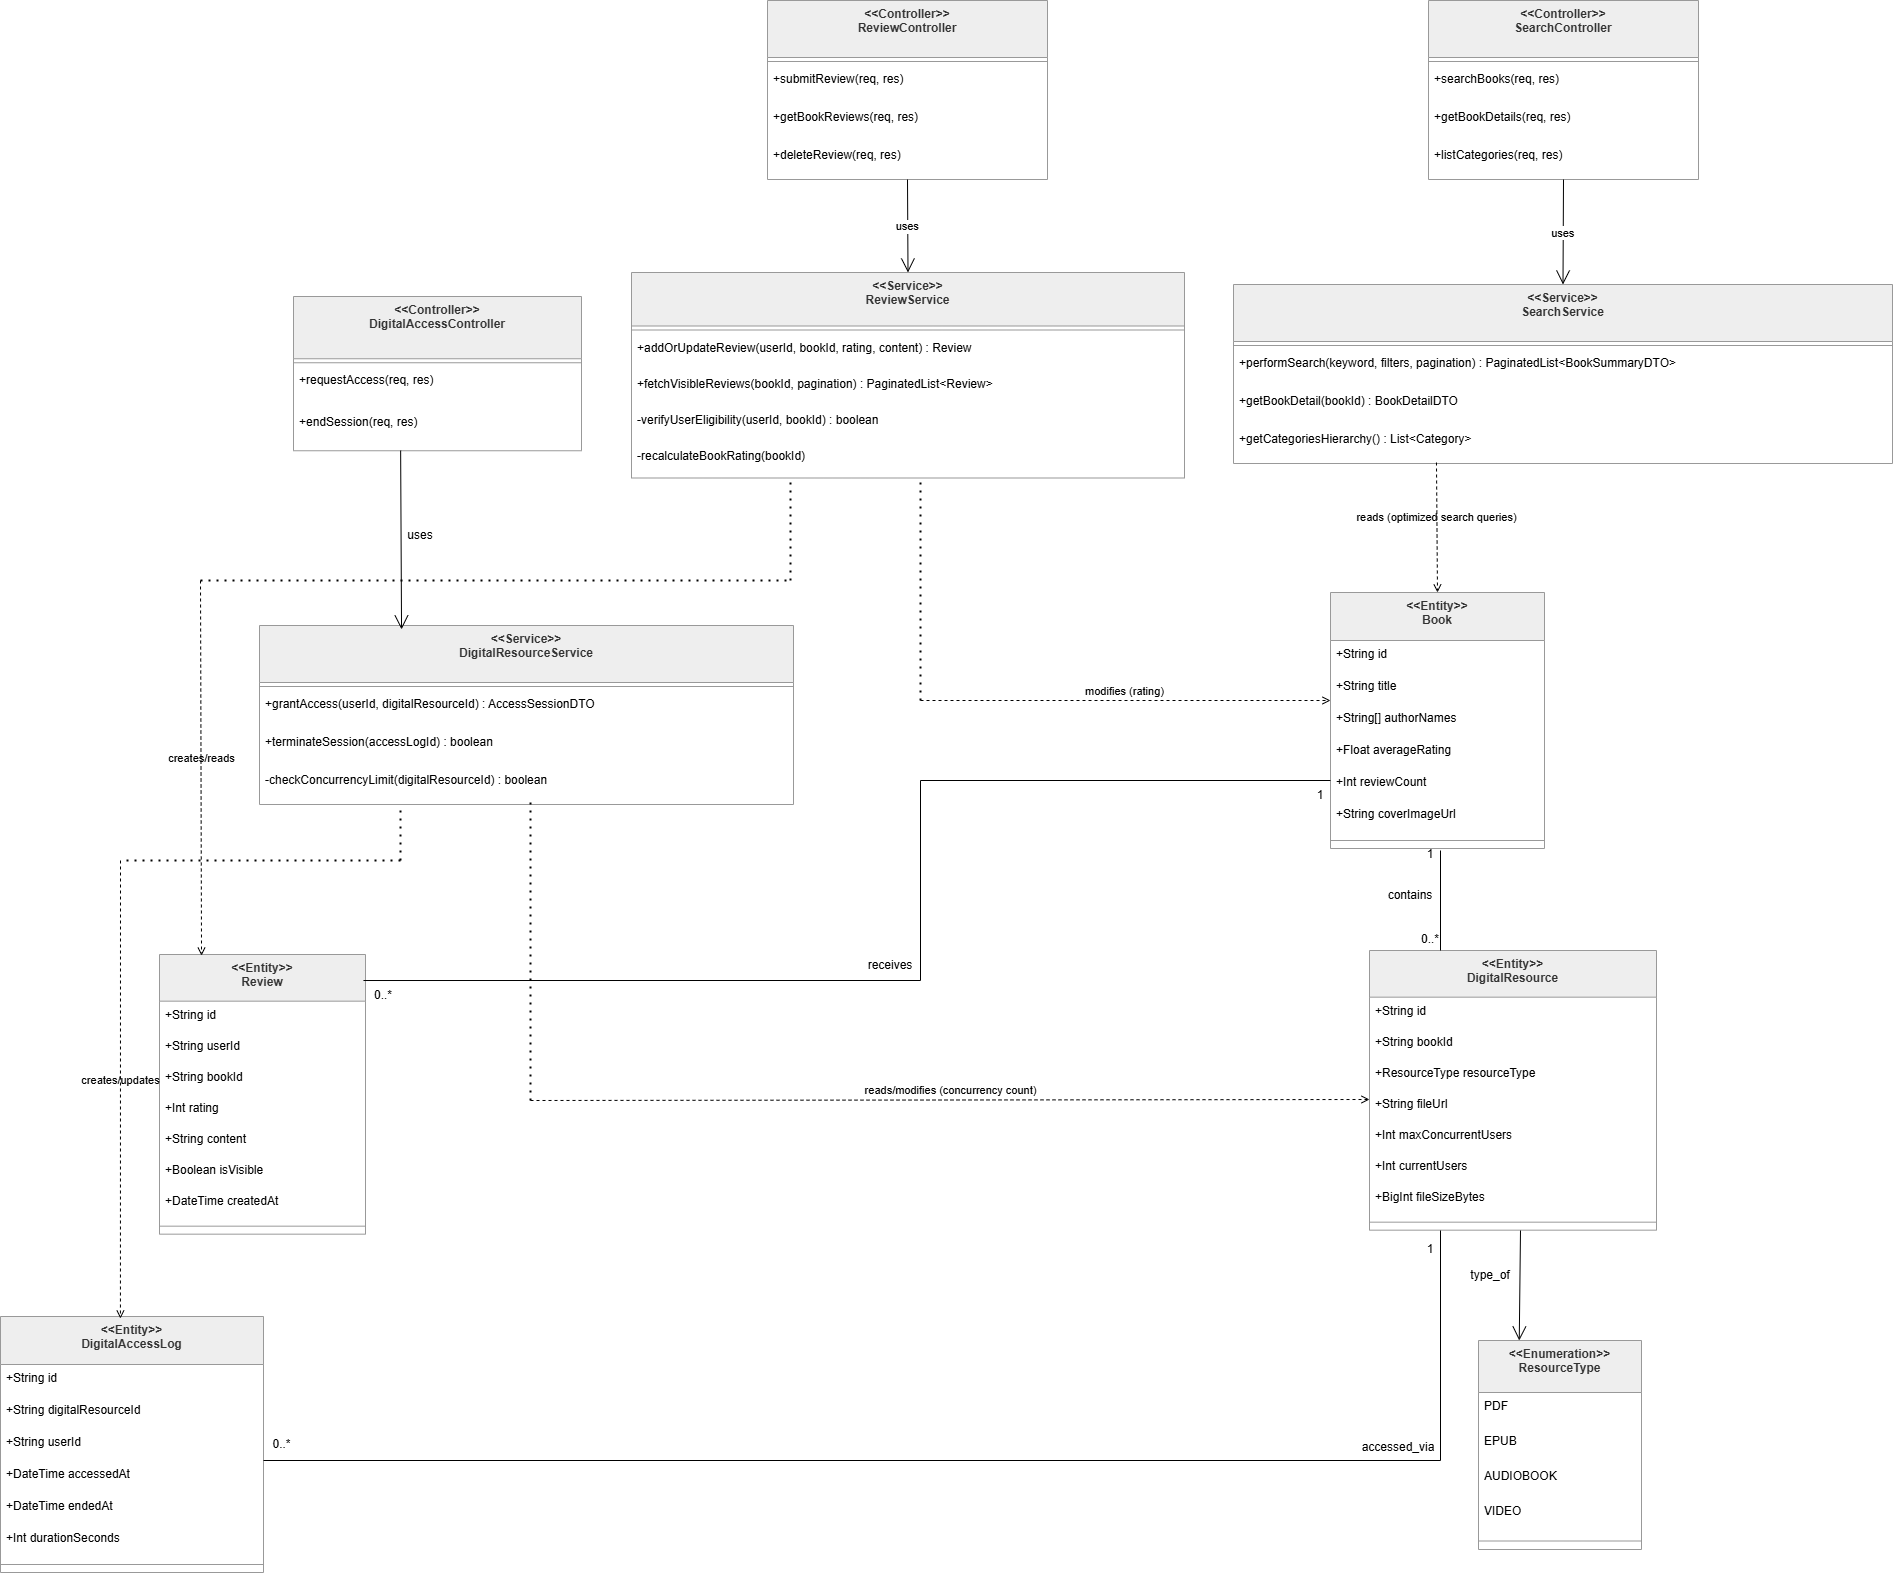
\includegraphics[width=0.6\linewidth]{Images/truycapvakhaithactainguyen.png}
    \vspace{10pt}
    \caption{Sơ đồ lớp Tìm kiếm và khai thác tài nguyên}
    \label{fig:class_exploration}
\end{figure}

Sơ đồ lớp phân hệ này được thiết kế nhằm để thể hiện việc mô hình hóa các đối tượng trong phân hệ \textbf{Tìm kiếm và khai thác tài nguyên} bao gồm các thuộc tính và các phương thức xử lý chính.

Đầu tiên, phân hệ này liên kết trực tiếp với thực thể cốt lõi là \texttt{Book} chứa các thuộc tính như \texttt{id}, \texttt{title}, \texttt{authorNames}, \texttt{averageRating}, \texttt{reviewCount}, và \texttt{coverImageUrl}. Để mở rộng khả năng cung cấp tài liệu số, thực thể \texttt{Book} có mối quan hệ association với thực thể \texttt{DigitalResource} (Tài nguyên số) theo tỷ lệ $1 - 0..*$, thể hiện một đầu sách có thể đính kèm nhiều định dạng tài nguyên điện tử khác nhau. Lớp \texttt{DigitalResource} lưu trữ các thông tin chi tiết bao gồm \texttt{id}, \texttt{bookId}, \texttt{fileUrl}, dung lượng tệp (\texttt{fileSizeBytes}), giới hạn số người truy cập đồng thời (\texttt{maxConcurrentUsers}), và số người hiện đang truy cập (\texttt{currentUsers}). Định dạng của tài nguyên này được cấu trúc qua mối quan hệ association với danh mục \texttt{ResourceType} bao gồm các kiểu dữ liệu: \texttt{PDF}, \texttt{EPUB}, \texttt{AUDIOBOOK}, và \texttt{VIDEO}.

Bên cạnh đó, nhằm phục vụ nhu cầu phản hồi và lưu vết khai thác của độc giả, hệ thống thiết kế thêm hai thực thể phụ thuộc. Thực thể thứ nhất là \texttt{Review} (Đánh giá) chứa các thuộc tính \texttt{id}, \texttt{userId}, \texttt{bookId}, điểm số (\texttt{rating}), nội dung (\texttt{content}), và trạng thái hiển thị (\texttt{isVisible}). Thực thể \texttt{Review} có quan hệ association với \texttt{Book} theo tỷ lệ $0..* - 1$, thể hiện một cuốn sách có thể nhận nhiều lượt đánh giá từ các người dùng khác nhau. Thực thể thứ hai là \texttt{DigitalAccessLog} (Nhật ký truy cập số) dùng để ghi vết thời gian sử dụng tài nguyên của độc giả, bao gồm các thuộc tính \texttt{id}, \texttt{digitalResourceId}, \texttt{userId}, \texttt{accessedAt}, \texttt{endedAt}, và thời lượng truy cập tính bằng giây (\texttt{durationSeconds}). Thực thể này có mối quan hệ association $0..* - 1$ với \texttt{DigitalResource}.

Về mặt kiến trúc và luồng điều hướng nghiệp vụ, phân hệ được chia tách thành ba luồng xử lý riêng biệt tương ứng với các tầng Controller và Service chuyên trách:

Đối với luồng nghiệp vụ Tìm kiếm và Tra cứu, lớp \texttt{SearchController} sử dụng lớp \texttt{SearchService} để thực hiện các phương thức xử lý chính bao gồm: tìm kiếm sách nâng cao (\texttt{performSearch}), xem chi tiết thông tin sách (\texttt{getBookDetail}), và lấy cấu trúc phân cấp danh mục (\texttt{getCategoriesHierarchy}). Lớp \texttt{SearchService} thực hiện mối quan hệ đọc dữ liệu trực tiếp từ thực thể \texttt{Book} thông qua các câu lệnh truy vấn đã được tối ưu hóa hiệu năng.

Đối với luồng nghiệp vụ Đánh giá (Review), lớp \texttt{ReviewController} sử dụng lớp \texttt{ReviewService} để hiện thực hóa các chức năng: gửi hoặc cập nhật đánh giá (\texttt{addOrUpdateReview}), lấy danh sách các đánh giá hợp lệ (\texttt{fetchVisibleReviews}), và xóa đánh giá (\texttt{deleteReview}). Đặc biệt, khi có một đánh giá mới được tạo hoặc cập nhật, lớp \texttt{ReviewService} sẽ gọi hàm nội bộ \texttt{recalculateBookRating(bookId)} nhằm tính toán lại điểm số trung bình và cập nhật trực tiếp thuộc tính \texttt{averageRating} trên thực thể \texttt{Book}. Đồng thời, dịch vụ này cũng thực hiện kiểm tra quyền hạn của người dùng thông qua hàm \texttt{verifyUserEligibility(userId, bookId)} trước khi cho phép ghi dữ liệu vào thực thể \texttt{Review}.

Đối với luồng nghiệp vụ Khai thác tài nguyên số, lớp \texttt{DigitalAccessController} sử dụng lớp \texttt{DigitalResourceService} để điều phối việc đọc tài liệu trực tuyến của độc giả qua hai hàm xử lý chính là yêu cầu truy cập (\texttt{requestAccess}) và kết thúc phiên đọc (\texttt{endSession}). Nhằm ngăn chặn tình trạng quá tải và vi phạm bản quyền tài liệu, lớp \texttt{DigitalResourceService} tích hợp hàm kiểm tra logic \texttt{checkConcurrencyLimit(digitalResourceId)}. Dịch vụ này có mối quan hệ trực tiếp để tạo mới hoặc cập nhật các phiên ghi vết trên thực thể \texttt{DigitalAccessLog}, đồng thời tăng giảm số lượng người dùng trực tuyến theo thời gian thực trên thực thể \texttt{DigitalResource}.

\subsubsection{Trợ lý ảo AI và gợi ý}

\begin{figure}[H]
    \centering
    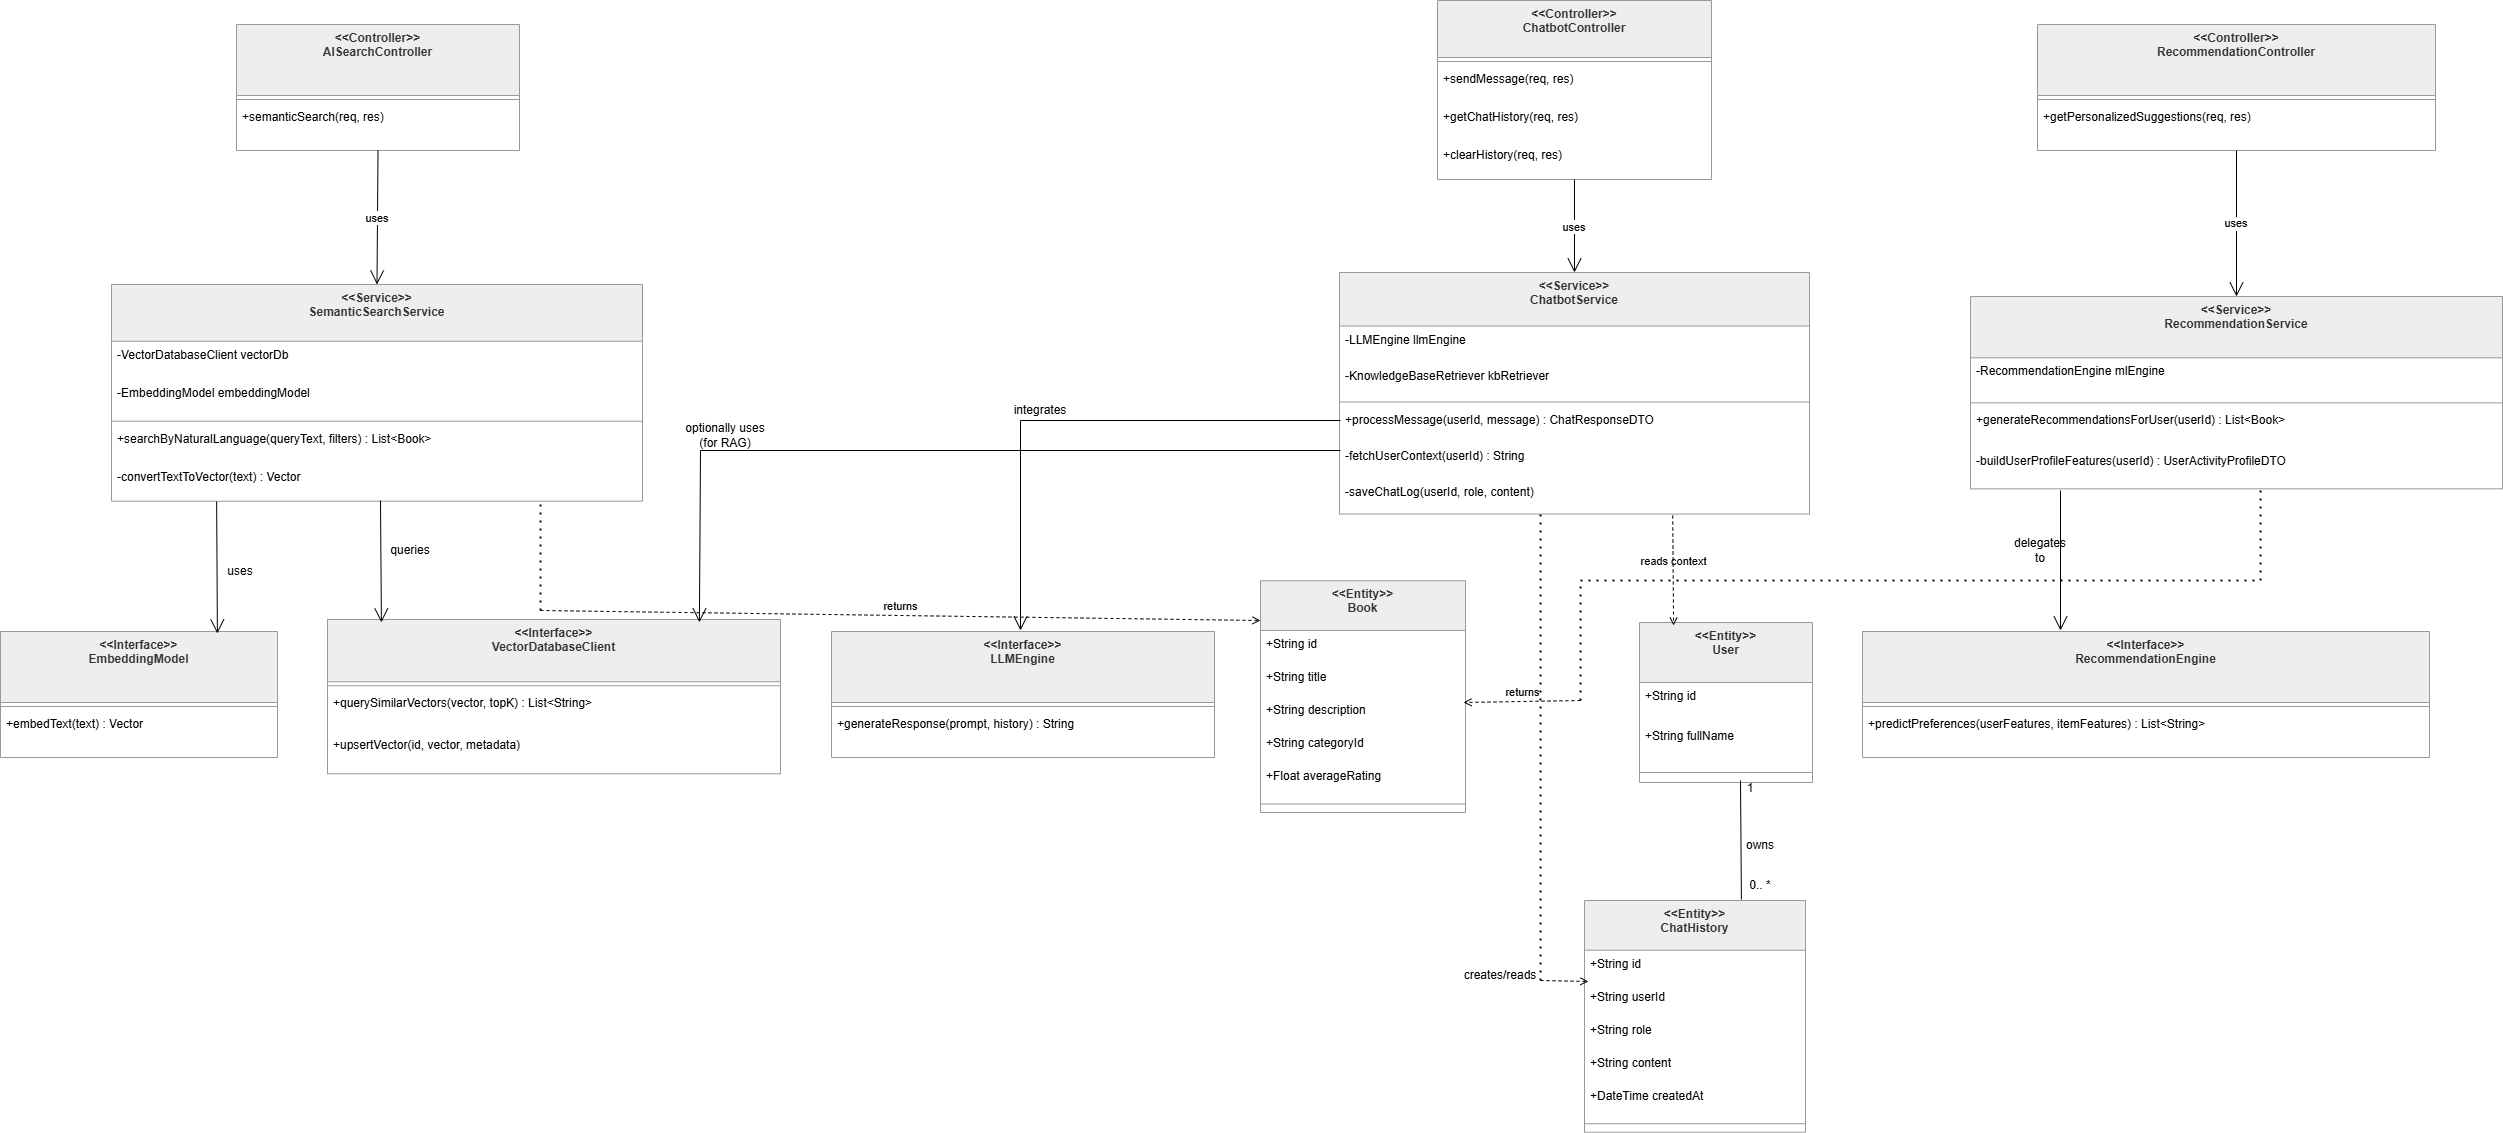
\includegraphics[width=0.6\linewidth]{Images/AI.png}
    \vspace{10pt}
    \caption{Sơ đồ lớp Trợ lý ảo AI và gợi ý}
    \label{fig:class_ai}
\end{figure}

Sơ đồ lớp phân hệ này được thiết kế nhằm để thể hiện việc mô hình hóa các đối tượng trong phân hệ các tính năng thông minh ứng dụng trí tuệ nhân tạo (\textbf{AI Search, Chatbot và Recommendation}) bao gồm các thuộc tính và các phương thức xử lý chính.

Đầu tiên, phân hệ này tiếp tục kế thừa và liên kết chặt chẽ với thực thể \texttt{User} từ hệ thống cốt lõi để thực hiện việc cá nhân hóa các phản hồi và gợi ý. Bên cạnh đó, hệ thống xuất hiện một thực thể nền tảng quan trọng khác là \texttt{Book} chứa các thông tin như \texttt{id}, \texttt{title}, \texttt{description}, \texttt{categoryId}, và \texttt{averageRating}. 

Về mặt cấu trúc vận hành, sơ đồ lớp chia rõ ràng các tính năng thông minh thành ba luồng nghiệp vụ độc lập nhưng có sự tương tác và hỗ trợ lẫn nhau:

Đối với luồng nghiệp vụ Tìm kiếm ngữ nghĩa (Semantic Search), lớp \texttt{AISearchController} sử dụng dịch vụ của lớp \texttt{SemanticSearchService}. Phương thức xử lý chính tại đây là \texttt{searchByNaturalLanguage(queryText, filters)} trả về một danh sách các đối tượng \texttt{Book}. Để hiện thực hóa việc tìm kiếm bằng ngôn ngữ tự nhiên, lớp \texttt{SemanticSearchService} có mối quan hệ association với hai giao tiếp (interface) cốt lõi là \texttt{EmbeddingModel} và \texttt{VectorDatabaseClient}.

Đối với luồng nghiệp vụ Trợ lý ảo (AI Chatbot), lớp \texttt{ChatbotController} sử dụng lớp \texttt{ChatbotService} để điều phối các tác vụ giao tiếp với người dùng bao gồm gửi tin nhắn (\texttt{sendMessage}), lấy lịch sử trò chuyện (\texttt{getChatHistory}), và xóa lịch sử cuộc gọi (\texttt{clearHistory}). Lớp \texttt{ChatbotService} tích hợp trực tiếp giao tiếp \texttt{LLMEngine} với phương thức chính là \texttt{generateResponse(prompt, history)} nhằm tạo ra văn bản trả lời tự nhiên. Không chỉ vậy, để phục vụ cho kỹ thuật tìm kiếm thực tế tăng cường (RAG), lớp \texttt{ChatbotService} còn có mối quan hệ phụ thuộc tới lớp \texttt{VectorDatabaseClient} để truy vấn ngữ cảnh từ sách, đồng thời đọc dữ liệu ngữ cảnh từ thực thể \texttt{User} thông qua hàm \texttt{fetchUserContext(userId)}. Toàn bộ các đoạn hội thoại giữa người dùng và AI sẽ được lưu vết trực tiếp vào thực thể \texttt{ChatHistory}, nơi có mối quan hệ association $1 - 0..*$ với thực thể \texttt{User}.

Đến với luồng nghiệp vụ Hệ thống gợi ý (Recommendation System), lớp \texttt{RecommendationController} sử dụng lớp \texttt{RecommendationService} thông qua phương thức \texttt{getPersonalizedSuggestions(req, res)} để cung cấp các đề xuất sách mang tính cá nhân hóa cao cho độc giả. Lớp \texttt{RecommendationService} này chịu trách nhiệm trích xuất dữ liệu hành vi của người dùng thông qua hàm \texttt{buildUserProfileFeatures(userId)} nhằm trả về một đối tượng chuyển đổi dữ liệu \texttt{UserActivityProfileDTO}, sau đó thực hiện ủy quyền xuống giao tiếp \texttt{RecommendationEngine}. Giao tiếp \texttt{RecommendationEngine} sở hữu phương thức xử lý chính là \texttt{predictPreferences(userFeatures, itemFeatures)} để tính toán và trả về một danh sách mã định danh các cuốn sách phù hợp nhất, từ đó giúp lớp \texttt{RecommendationService} sinh ra danh sách dữ liệu thực thể \texttt{Book} gửi ngược lại cho người dùng.

\subsubsection{Thông báo và truyền thông}

\begin{figure}[H]
    \centering
    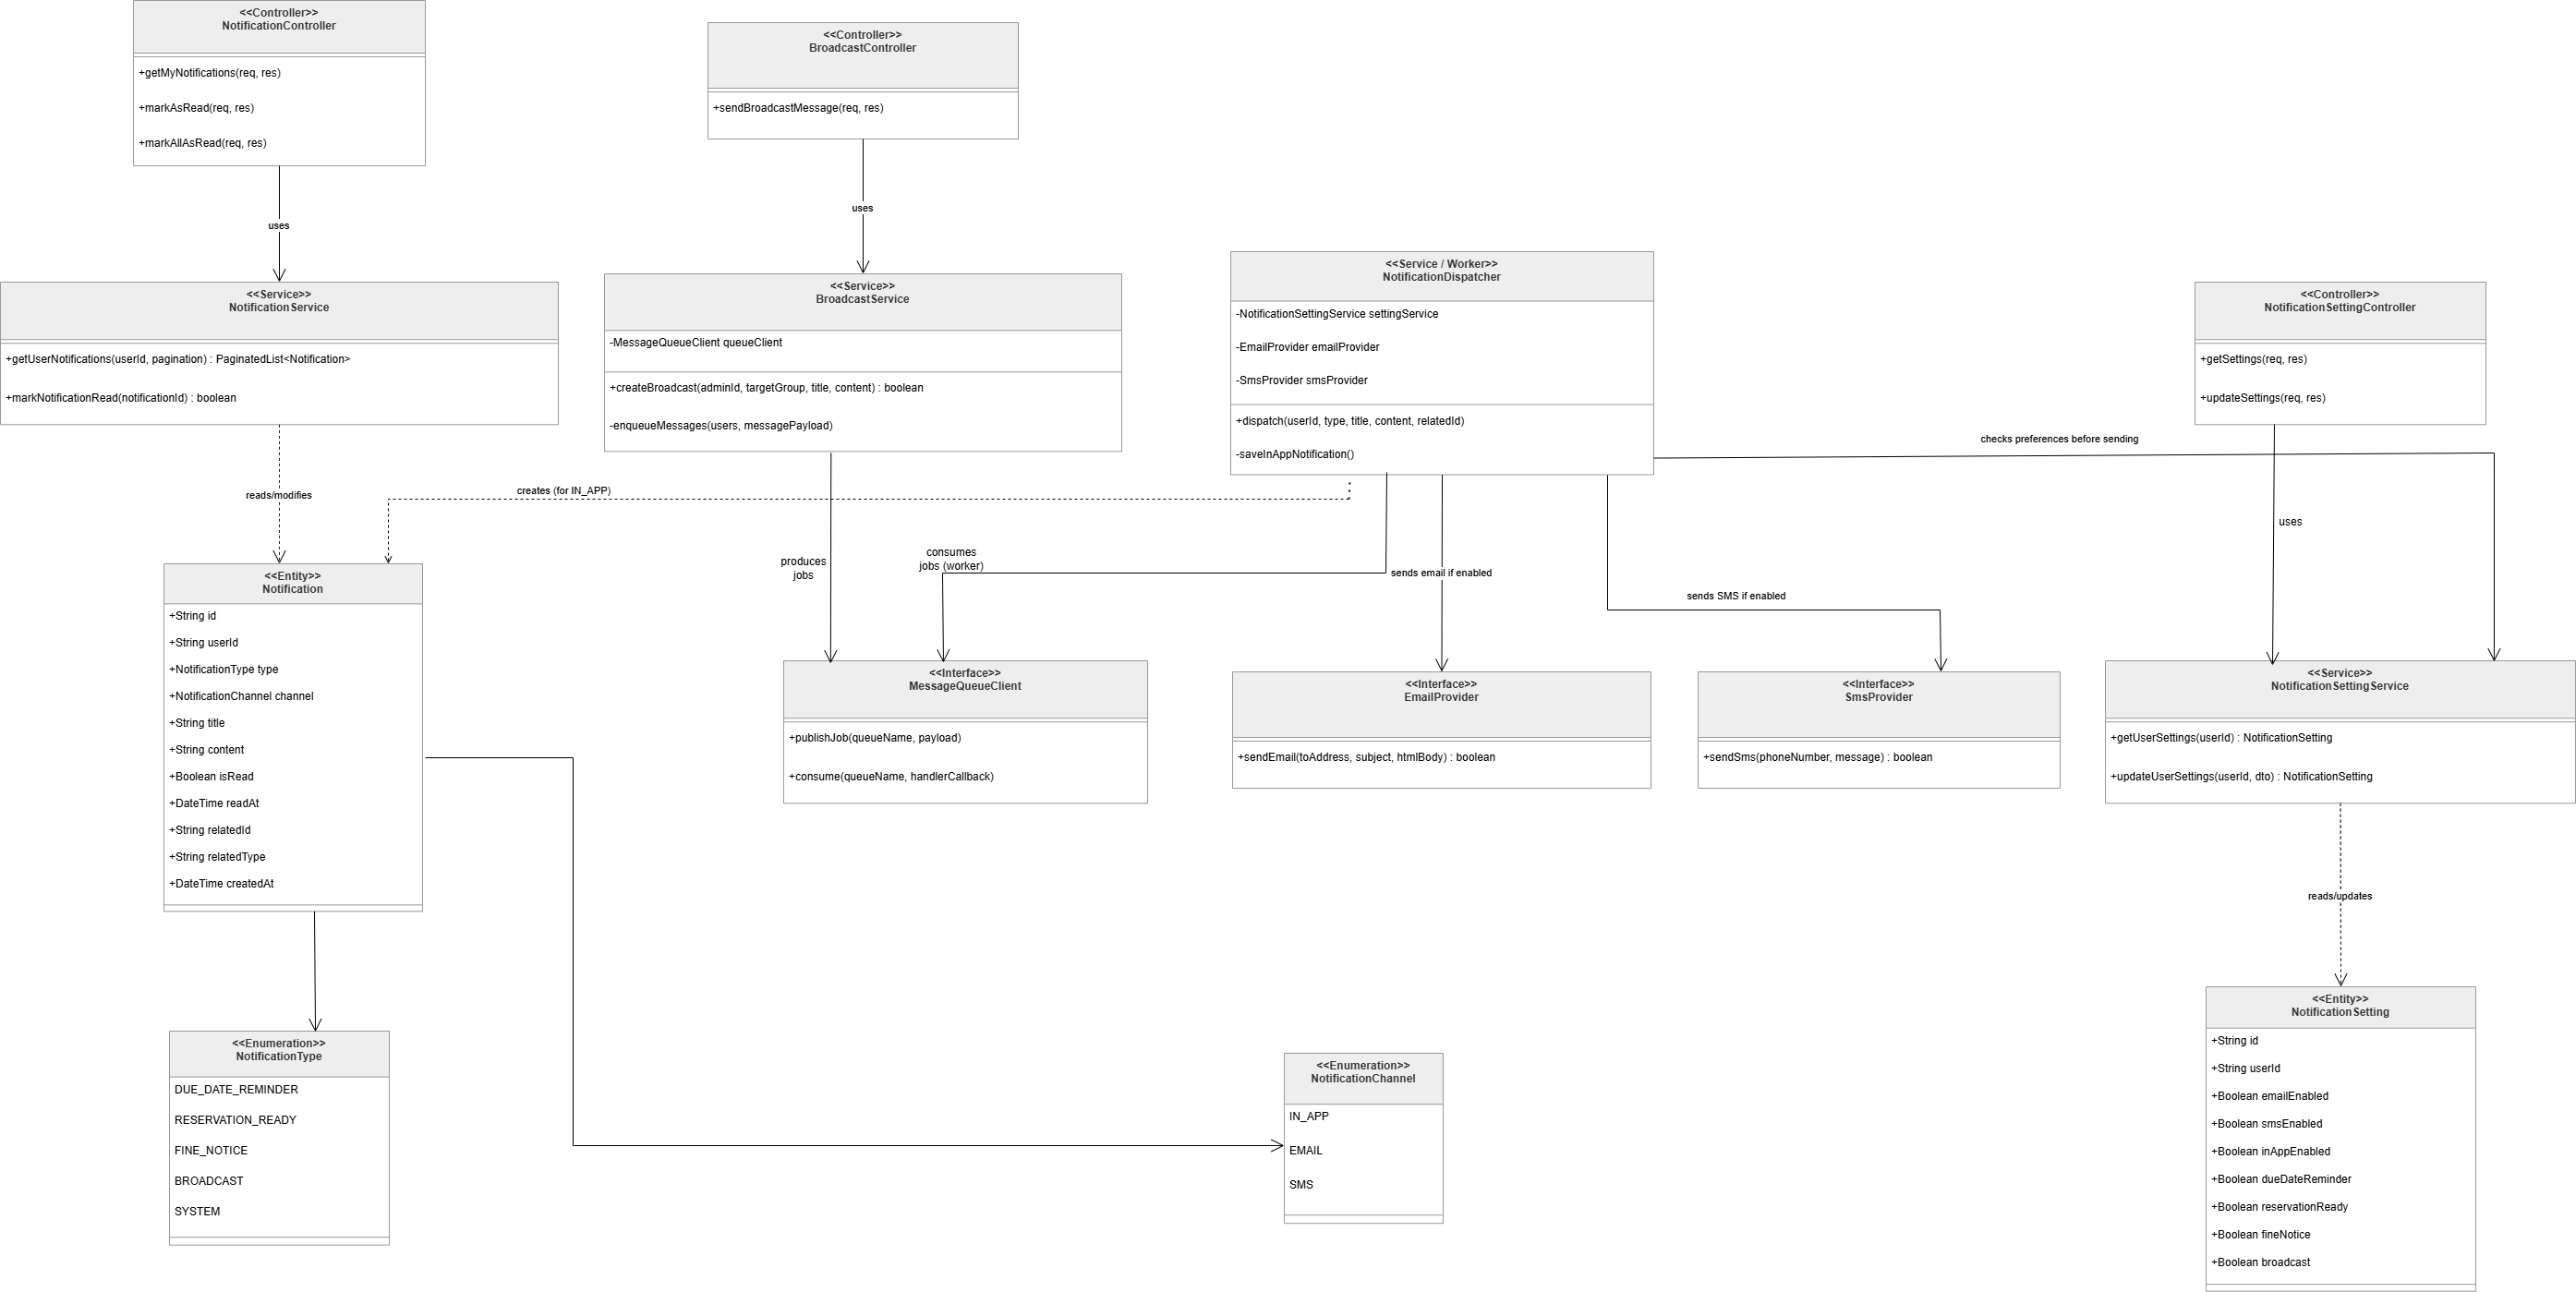
\includegraphics[width=0.6\linewidth]{Images/thongbao.png}
    \vspace{10pt}
    \caption{Sơ đồ lớp Thông báo và truyền thông}
    \label{fig:class_notification}
\end{figure}

Sơ đồ lớp phân hệ này được thiết kế nhằm để thể hiện việc mô hình hóa các đối tượng trong \textbf{Phân hệ Thông báo và truyền thông} bao gồm các thuộc tính và các phương thức xử lý chính.

Đầu tiên, trung tâm dữ liệu lưu trữ của phân hệ này tập trung vào thực thể \texttt{Notification} (Thông báo) và thực thể \texttt{NotificationSetting} (Cấu hình thông báo). Thực thể \texttt{Notification} chứa các thuộc tính cốt lõi bao gồm \texttt{id}, \texttt{userId}, \texttt{title}, \texttt{content}, trạng thái đã đọc \texttt{isRead}, cùng các mốc thời gian liên quan. Để phân loại tin nhắn, thực thể \texttt{Notification} có mối quan hệ association với hai danh mục là \texttt{NotificationType} (gồm các loại: \texttt{DUE\_DATE\_REMINDER}, \texttt{RESERVATION\_READY}, \texttt{FINE\_NOTICE}, \texttt{BROADCAST}, \texttt{SYSTEM}) và \texttt{NotificationChannel} (gồm các kênh: \texttt{IN\_APP}, \texttt{EMAIL}, \texttt{SMS}). Đối với thực thể \texttt{NotificationSetting}, lớp này lưu trữ các tùy chọn bật/tắt nhận tin của từng người dùng qua các trường dữ liệu Boolean như \texttt{emailEnabled}, \texttt{smsEnabled}, \texttt{inAppEnabled}, giúp cá nhân hóa quyền nhận thông báo của độc giả.

Về mặt kiến trúc và luồng điều phối nghiệp vụ, phân hệ được phân rã thành các luồng tương tác thông qua hệ thống Controller, Service và thành phần xử lý bất đồng bộ (Worker):

Đối với luồng cấu hình của người dùng, lớp \texttt{NotificationSettingController} sử dụng lớp \texttt{NotificationSettingService} để thực hiện các phương thức xử lý chính bao gồm lấy cấu hình hiện tại (\texttt{getNotificationSettings}) và cập nhật cấu hình mới (\texttt{updateNotificationSettings}). Lớp dịch vụ này thực hiện mối quan hệ đọc và cập nhật dữ liệu trực tiếp trên thực thể \texttt{NotificationSetting}.

Đối với luồng tiếp nhận thông báo thông thường, lớp \texttt{NotificationController} điều phối qua lớp \texttt{NotificationService} để hiện thực hóa các chức năng lấy danh sách thông báo phân trang của người dùng (\texttt{getUserNotifications}) và đánh dấu thông báo đã đọc (\texttt{markNotificationAsRead}). Lớp \texttt{NotificationService} có mối quan hệ trực tiếp để truy vấn và cập nhật trạng thái trên thực thể \texttt{Notification}.

Đối với luồng gửi tin nhắn quảng bá diện rộng từ quản trị viên, lớp \texttt{BroadcastController} sử dụng lớp \texttt{BroadcastService} thông qua hàm xử lý \texttt{createBroadcast(adminId, targetGroup, title, content)} để tạo thông báo cho một nhóm đối tượng. Để đảm bảo hiệu năng hệ thống không bị ảnh hưởng khi gửi tin nhắn số lượng lớn, lớp \texttt{BroadcastService} không thực hiện gửi trực tiếp mà đẩy các tác vụ này vào hàng đợi thông qua mối quan hệ tạo việc làm với giao tiếp \texttt{MessageQueueClient}. Giao tiếp này sở hữu hàm \texttt{publishJob} và \texttt{consumeQueue}. Sau đó, \texttt{BroadcastService} cũng tiến hành lưu vết thông báo lưu trữ vào thực thể \texttt{Notification}.

Cuối cùng, xử lý tác vụ gửi tin của phân hệ là thành phần \texttt{NotificationDispatcher} đóng vai trò như một Service/Worker bất đồng bộ. Thành phần này liên tục tiêu thụ các tác vụ từ hàng đợi của giao tiếp \texttt{MessageQueueClient}. Trước khi tiến hành gửi tin, \texttt{NotificationDispatcher} có mối quan hệ phụ thuộc để kiểm tra chéo tùy chọn ưu tiên của người dùng với lớp \texttt{NotificationSettingService}. Nếu người dùng cho phép, điều phối viên này sẽ hiện thực hóa việc gửi tin thông qua phương thức \texttt{dispatch(userId, type, title, content, relatedId)}, đồng thời gọi các dịch vụ hạ tầng tương ứng bao gồm thực hiện lưu thông báo ứng dụng nội bộ (\texttt{saveInAppNotification}), gọi giao tiếp \texttt{EmailProvider} để gửi thư điện tử qua hàm \texttt{sendEmail}, và gọi giao tiếp \texttt{SmsProvider} để gửi tin nhắn viễn thông qua hàm \texttt{sendSms}.

\subsubsection{Quản trị hệ thống}

\begin{figure}[H]
    \centering
    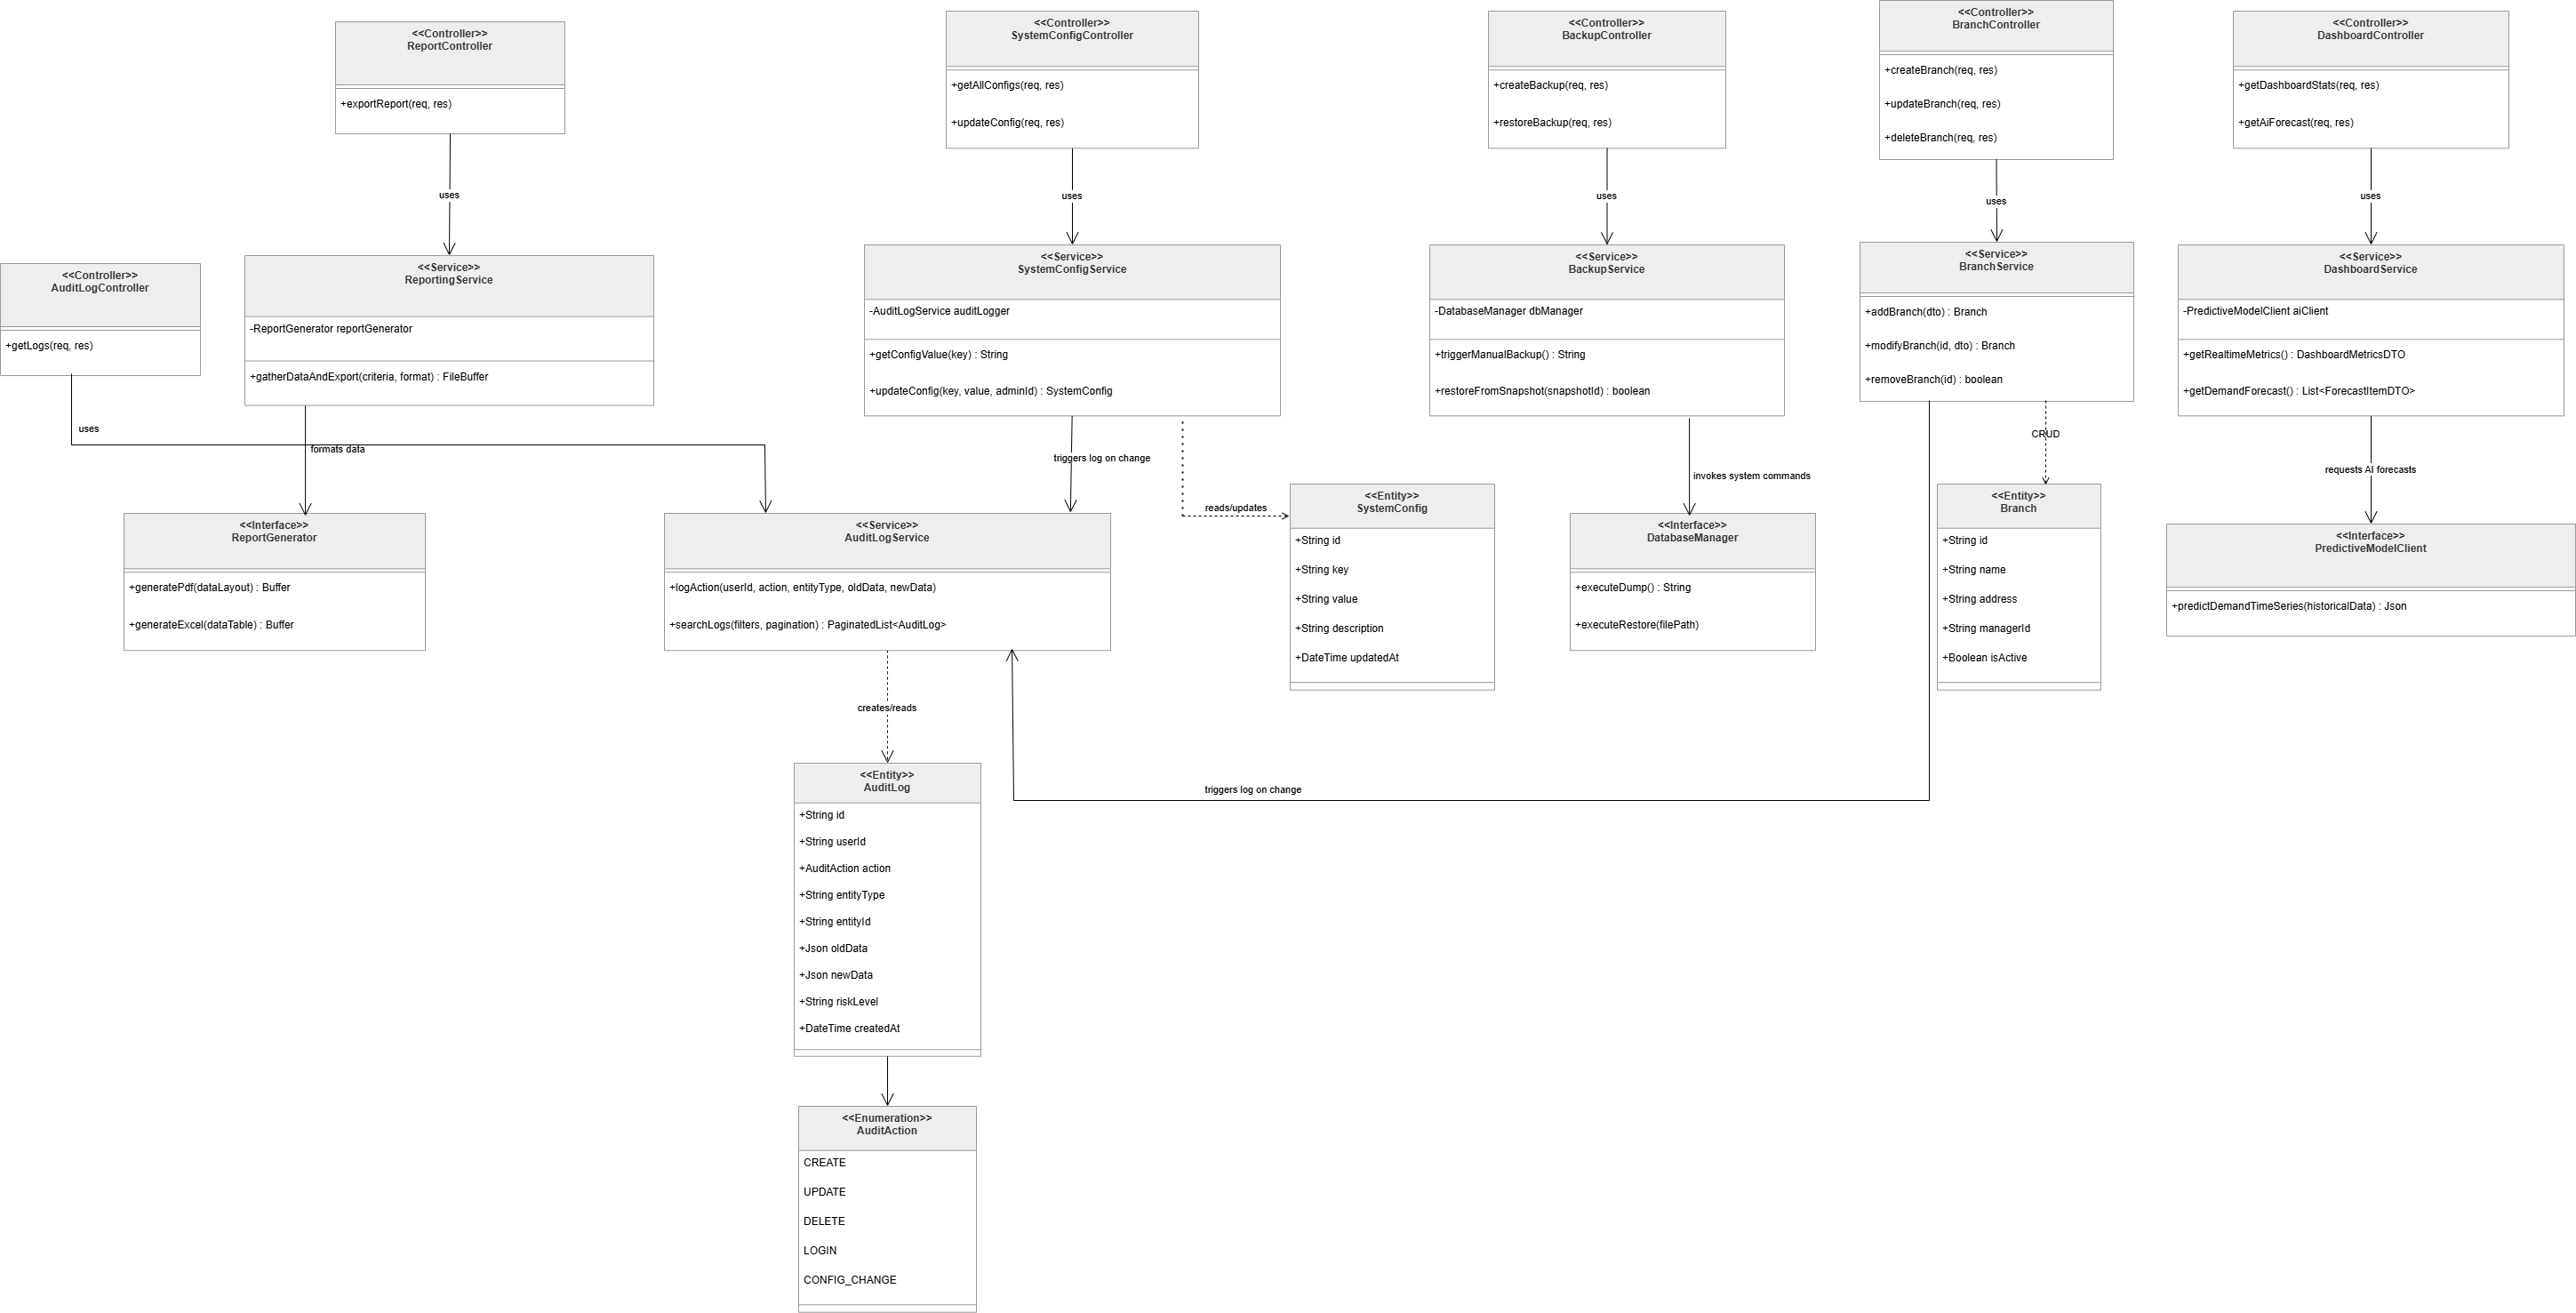
\includegraphics[width=0.6\linewidth]{Images/baocaovaquantri.png}
    \vspace{10pt}
    \caption{Sơ đồ lớp Quản trị hệ thống}
    \label{fig:class_admin}
\end{figure}

Sơ đồ lớp phân hệ này được thiết kế nhằm để thể hiện việc mô hình hóa các đối tượng trong \textbf{Quản trị hệ thống} bao gồm các thuộc tính và các phương thức xử lý chính.

Đầu tiên, về mặt lưu trữ cấu trúc dữ liệu nền tảng, phân hệ này sở hữu ba thực thể độc lập phục vụ cho các tác vụ cấu hình và quản trị cơ sở hạ tầng. Thực thể thứ nhất là \texttt{AuditLog} (Nhật ký kiểm toán) chứa các thuộc tính quan trọng để lưu vết hành vi như \texttt{id}, \texttt{userId}, \texttt{action}, \texttt{entityType}, \texttt{entityId}, \texttt{oldData}, \texttt{newData}, mức độ rủi ro (\texttt{riskLevel}) và ngày tạo. Để chuẩn hóa các hành động kiểm toán, thực thể này liên kết trực tiếp với danh mục trạng thái \texttt{AuditAction} bao gồm: \texttt{CREATE}, \texttt{UPDATE}, \texttt{DELETE}, \texttt{LOGIN}, và \texttt{CONFIG\_CHANGE}. Thực thể thứ hai là \texttt{SystemConfig} (Cấu hình hệ thống) dùng để lưu trữ các tham số vận hành động dưới dạng cặp khóa - giá trị (\texttt{key}, \texttt{value}, \texttt{description}). Thực thể thứ ba là \texttt{Branch} (Chi nhánh thư viện) đại diện cho các cơ sở vật lý trong mạng lưới, bao gồm \texttt{id}, \texttt{name}, \texttt{address}, \texttt{managerId}, và trạng thái hoạt động \texttt{isActive}.

Về mặt kiến trúc và luồng điều hướng nghiệp vụ quản trị, phân hệ được phân rã thành các cụm tính năng chuyên biệt sử dụng mô hình kết hợp giữa xử lý dữ liệu truyền thống và dự báo thông minh:

Đối với luồng nghiệp vụ Kiểm toán và Kết xuất báo cáo, lớp \texttt{AuditLogController} phối hợp cùng lớp \texttt{AuditLogService} để cung cấp tính năng tra cứu và tìm kiếm nâng cao kết hợp phân trang dữ liệu nhật ký qua hàm \texttt{searchLogs}. Lớp \texttt{AuditLogService} có mối quan hệ trực tiếp để tạo mới hoặc đọc dữ liệu trên thực thể \texttt{AuditLog}. Song song với đó, lớp \texttt{ReportController} sử dụng \texttt{ReportingService} nhằm thực hiện gom cụm dữ liệu báo cáo (\texttt{gatherDataAndExport}). Để thực hiện định dạng tài liệu, dịch vụ này liên kết phụ thuộc với giao tiếp \texttt{ReportGenerator} chứa các hàm kết xuất dữ liệu gốc sang tệp tin nhị phân (\texttt{generatePdf} và \texttt{generateExcel}), sau đó đẩy dữ liệu nhật ký kiểm toán sang cho \texttt{AuditLogService} lưu vết.

Đối với luồng nghiệp vụ Cấu hình và Sao lưu hệ thống, lớp \texttt{SystemConfigController} sử dụng \texttt{SystemConfigService} để thực hiện đọc và cập nhật các tham số hệ thống (\texttt{getConfigValue}, \texttt{updateConfigKey}). Khi có bất kỳ sự thay đổi cấu hình nào, dịch vụ này sẽ tự động kích hoạt ghi nhận nhật ký sang \texttt{AuditLogService}. Ngoài ra, việc an toàn dữ liệu được điều phối bởi lớp \texttt{BackupController} và \texttt{BackupService} thông qua các phương thức kích hoạt sao lưu thủ công (\texttt{triggerManualBackup}) hoặc khôi phục từ ảnh chụp dữ liệu (\texttt{restoreFromSnapshot}). Lớp \texttt{BackupService} sẽ ủy quyền gọi các lệnh hệ thống cấp thấp thông qua giao tiếp \texttt{DatabaseManager} sở hữu hai phương thức \texttt{executeDump} và \texttt{executeRestore}.

Đối với luồng nghiệp vụ Quản lý chi nhánh, lớp \texttt{BranchController} sử dụng \texttt{BranchService} để thực thi toàn bộ các tác vụ CRUD quản trị mạng lưới cơ sở bao gồm thêm mới (\texttt{addBranch}), chỉnh sửa (\texttt{modifyBranch}) và ngưng hoạt động chi nhánh (\texttt{removeBranch}). Dịch vụ này có mối quan hệ tương tác và chỉnh sửa dữ liệu trực tiếp lên thực thể \texttt{Branch}, đồng thời phát tín hiệu lưu vết sang cho tầng kiểm toán.

Cuối cùng, luồng nghiệp vụ Giám sát và Dự báo thông minh được đảm nhiệm bởi cặp lớp \texttt{DashboardController} và \texttt{DashboardService}. Tầng dịch vụ này cung cấp các phương thức chính bao gồm lấy các chỉ số vận hành thời gian thực (\texttt{getRealtimeMetrics}) trả về cấu trúc \texttt{DashboardMetricsDTO}, và đưa ra các dự báo số lượng mượn trả (\texttt{getAiForecast}). Nhằm hiện thực hóa khả năng dự báo xu hướng tương lai, lớp \texttt{DashboardService} có mối quan hệ phụ thuộc gửi yêu cầu tính toán tới giao tiếp \texttt{PredictiveModelClient}. Giao tiếp thông minh này sở hữu phương thức xử lý chính là \texttt{predictDemandTimeSeries(historicalData)} để chạy các thuật toán học máy dựa trên dữ liệu lịch sử mượn trả, từ đó trả về kết quả dự báo chính xác giúp người quản trị tối ưu hóa kế hoạch phân phối sách giữa các chi nhánh.

\subsection{Sơ đồ hoạt động (Activity Diagram)}
\subsubsection{Đăng kí tài khoản}

\begin{figure}[H]
    \centering
    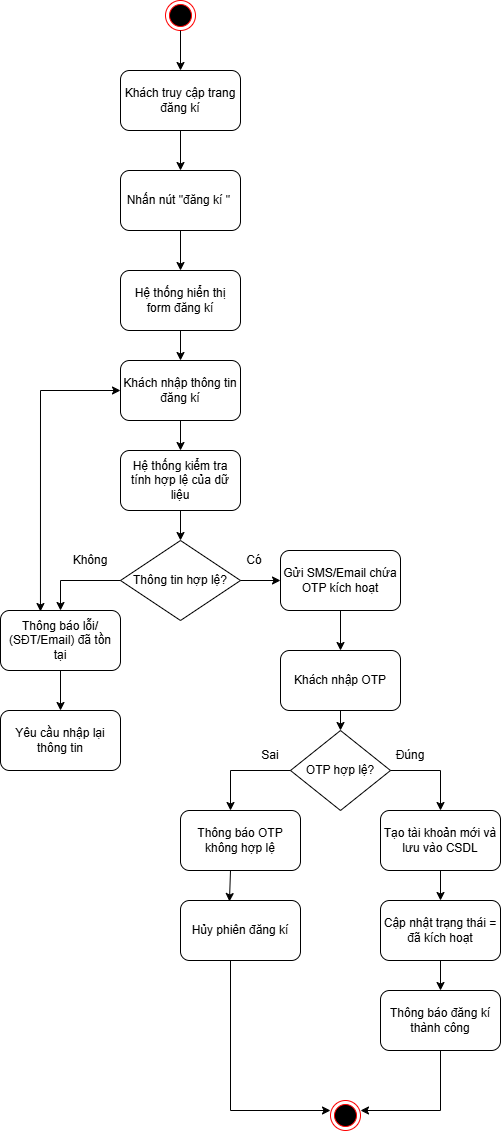
\includegraphics[width=0.6\linewidth]{Images/dangki.png}
    \vspace{10pt}
    \caption{Sơ đồ hoạt động đăng kí tài khoản}
    \label{fig:activity_register}
\end{figure}

\begin{enumerate}
    \item Khách truy cập vào trang đăng ký tài khoản.
    
    \item Hệ thống hiển thị biểu mẫu đăng ký.
    
    \item Khách nhập các thông tin đăng ký (Họ tên, Email/SĐT, Mật khẩu, \ldots).
    
    \item Hệ thống kiểm tra tính hợp lệ của dữ liệu đã nhập.
    
    \item Hệ thống kiểm tra Email/SĐT đã tồn tại trong cơ sở dữ liệu hay chưa.

    \item \textbf{Nhánh hợp lệ}
    \begin{itemize}
        \item Nếu thông tin hợp lệ, hệ thống gửi Email/SMS chứa mã OTP hoặc link kích hoạt tài khoản.
        
        \item Khách nhập mã OTP hoặc nhấn link kích hoạt.
        
        \item Hệ thống kiểm tra tính hợp lệ của OTP/link xác thực.
        
        \item Nếu OTP/link hợp lệ:
        \begin{itemize}
            \item Hệ thống tạo tài khoản mới.
            
            \item Hệ thống lưu thông tin tài khoản vào cơ sở dữ liệu.
            
            \item Hệ thống cập nhật trạng thái tài khoản thành ``Đã kích hoạt''.
            
            \item Hệ thống thông báo đăng ký thành công.
        \end{itemize}
    \end{itemize}

    \item \textbf{Nhánh không hợp lệ}
    \begin{itemize}
        \item Nếu thông tin đăng ký không hợp lệ hoặc Email/SĐT đã tồn tại:
        \begin{itemize}
            \item Hệ thống hiển thị thông báo lỗi.
            
            \item Yêu cầu người dùng nhập lại thông tin đăng ký.
        \end{itemize}

        \item Nếu OTP không hợp lệ:
        \begin{itemize}
            \item Hệ thống thông báo OTP không hợp lệ.
            
            \item Hệ thống hủy phiên đăng ký.
        \end{itemize}
    \end{itemize}
\end{enumerate}
\subsubsection{Đăng nhập hệ thống}

\begin{figure}[H]
    \centering
    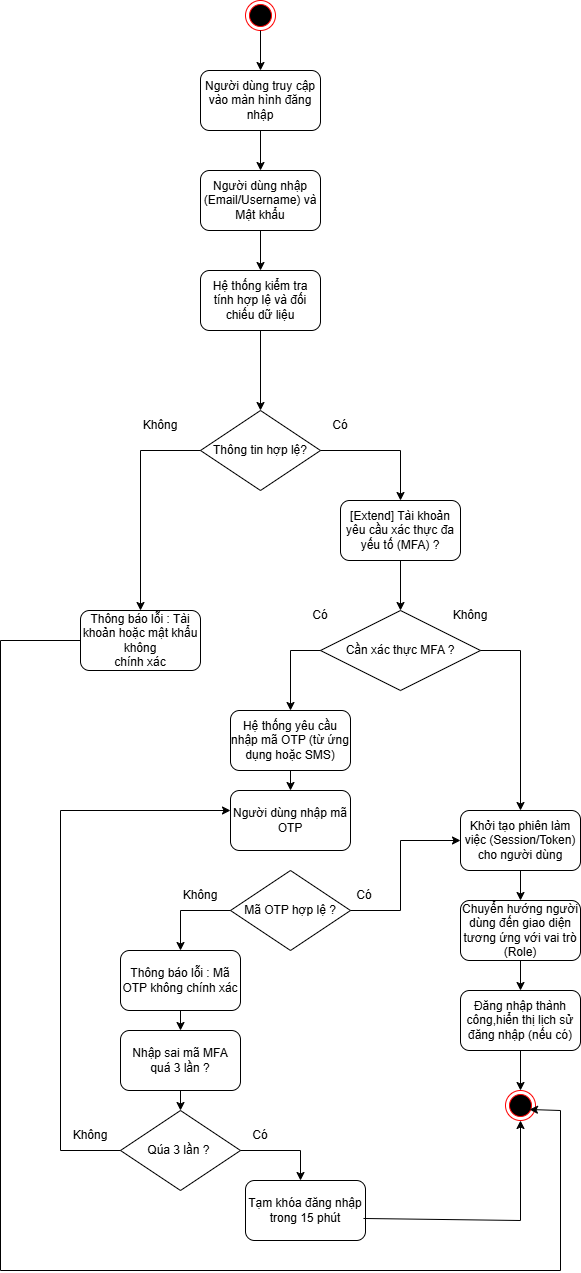
\includegraphics[width=0.6\linewidth]{Images/dangnhap.png}
    \vspace{10pt}
    \caption{Sơ đồ hoạt động đăng nhập hệ thống}
    \label{fig:activity_login}
\end{figure}

\begin{enumerate}
    \item Người dùng truy cập màn hình đăng nhập.
    
    \item Người dùng nhập Email/Username và Mật khẩu.
    
    \item Hệ thống kiểm tra tính hợp lệ và đối chiếu dữ liệu.

    \item Nếu thông tin đăng nhập không hợp lệ:
    \begin{itemize}
        \item Hệ thống hiển thị thông báo lỗi ``Tài khoản hoặc mật khẩu không chính xác''.
    \end{itemize}

    \item Nếu thông tin đăng nhập hợp lệ:
    \begin{itemize}
        \item Hệ thống kiểm tra tài khoản có yêu cầu xác thực đa yếu tố (MFA) hay không.
    \end{itemize}

    \item Nếu tài khoản yêu cầu MFA:
    \begin{itemize}
        \item Hệ thống yêu cầu người dùng nhập mã OTP (từ ứng dụng hoặc SMS).
        
        \item Người dùng nhập mã OTP.
        
        \item Hệ thống kiểm tra tính hợp lệ của mã OTP.
    \end{itemize}

    \item Nếu mã OTP không hợp lệ:
    \begin{itemize}
        \item Hệ thống hiển thị thông báo lỗi ``Mã OTP không chính xác''.
        
        \item Hệ thống kiểm tra số lần nhập sai MFA.
        
        \item Nếu người dùng nhập sai quá 3 lần:
        \begin{itemize}
            \item Hệ thống tạm khóa đăng nhập trong 15 phút.
        \end{itemize}
        
        \item Nếu chưa vượt quá 3 lần:
        \begin{itemize}
            \item Yêu cầu người dùng nhập lại mã OTP.
        \end{itemize}
    \end{itemize}

    \item Nếu mã OTP hợp lệ hoặc tài khoản không yêu cầu MFA:
    \begin{itemize}
        \item Hệ thống khởi tạo phiên làm việc (Session/Token) cho người dùng.
        
        \item Hệ thống chuyển hướng người dùng đến giao diện tương ứng với vai trò (Role).
        
        \item Hệ thống thông báo đăng nhập thành công và hiển thị lịch sử đăng nhập (nếu có).
    \end{itemize}
\end{enumerate}

\subsubsection{Đặt lại mật khẩu}

\begin{figure}[H]
    \centering
    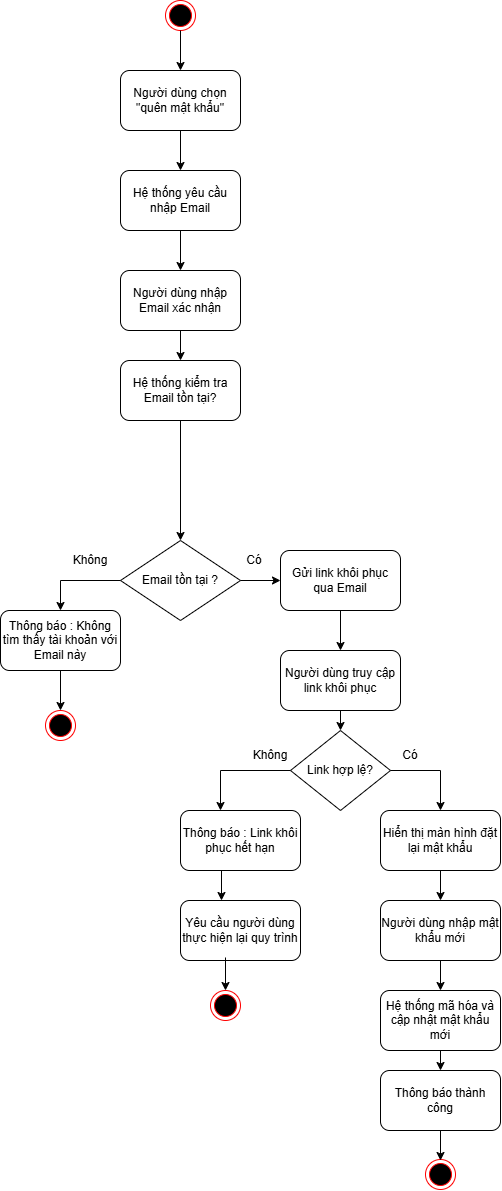
\includegraphics[width=0.6\linewidth]{Images/datlai.png}
    \vspace{10pt}
    \caption{Sơ đồ hoạt động đặt lại mật khẩu}
    \label{fig:activity_reset_password}
\end{figure}


\begin{enumerate}
    \item Người dùng chọn chức năng ``Quên mật khẩu''.
    
    \item Hệ thống yêu cầu người dùng nhập Email.
    
    \item Người dùng nhập Email xác nhận.
    
    \item Hệ thống kiểm tra Email có tồn tại trong hệ thống hay không.

    \item Nếu Email không tồn tại:
    \begin{itemize}
        \item Hệ thống hiển thị thông báo ``Không tìm thấy tài khoản với email này''.
    \end{itemize}

    \item Nếu Email tồn tại:
    \begin{itemize}
        \item Hệ thống gửi link khôi phục mật khẩu qua Email.
        
        \item Người dùng truy cập link khôi phục.
        
        \item Hệ thống kiểm tra tính hợp lệ của link khôi phục.
    \end{itemize}

    \item Nếu link khôi phục không hợp lệ hoặc đã hết hạn:
    \begin{itemize}
        \item Hệ thống hiển thị thông báo ``Link khôi phục hết hạn''.
        
        \item Yêu cầu người dùng thực hiện lại quy trình đặt lại mật khẩu.
    \end{itemize}

    \item Nếu link khôi phục hợp lệ:
    \begin{itemize}
        \item Hệ thống hiển thị màn hình đặt lại mật khẩu.
        
        \item Người dùng nhập mật khẩu mới.
        
        \item Hệ thống mã hóa và cập nhật mật khẩu mới.
        
        \item Hệ thống thông báo đặt lại mật khẩu thành công.
    \end{itemize}
\end{enumerate}

\subsubsection{Xem lịch sử mượn/trả}

\begin{figure}[H]
    \centering
    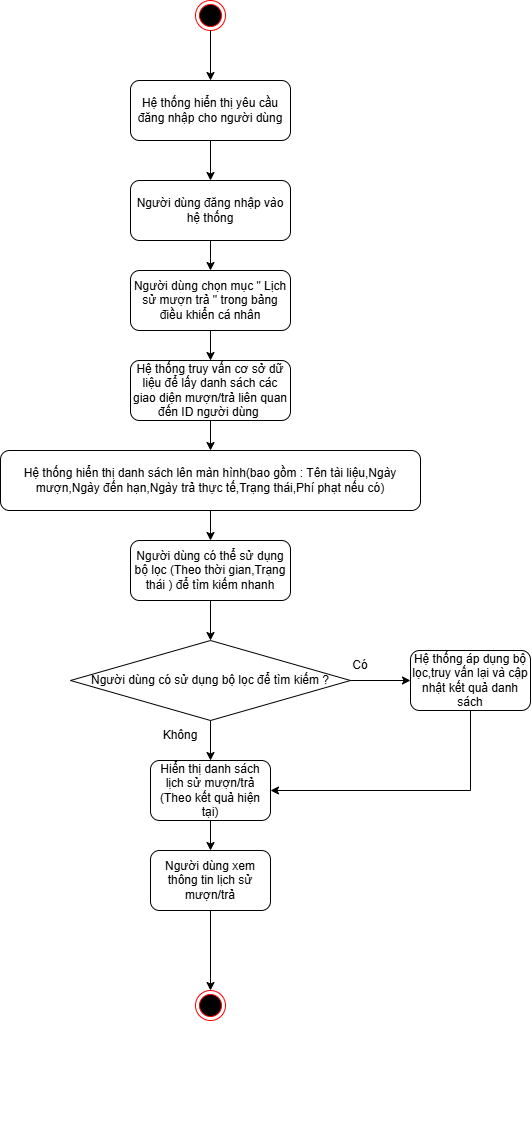
\includegraphics[width=0.6\linewidth]{Images/xemlichsu.png}
    \vspace{10pt}
    \caption{Sơ đồ hoạt động Xem lịch sử mượn/trả}
    \label{fig:activity_view_history}
\end{figure}
\begin{enumerate}
    \item Hệ thống hiển thị yêu cầu đăng nhập cho người dùng.
    
    \item Người dùng đăng nhập vào hệ thống.
    
    \item Người dùng chọn mục ``Lịch sử mượn/trả'' trong bảng điều khiển cá nhân.
    
    \item Hệ thống truy vấn cơ sở dữ liệu để lấy danh sách các giao dịch mượn/trả liên quan đến ID người dùng.
    
    \item Hệ thống hiển thị danh sách lịch sử mượn/trả lên màn hình, bao gồm:
    \begin{itemize}
        \item Tên tài liệu.
        \item Ngày mượn.
        \item Ngày đến hạn.
        \item Ngày trả thực tế.
        \item Trạng thái.
        \item Phí phạt (nếu có).
    \end{itemize}
    
    \item Người dùng có thể sử dụng bộ lọc để tìm kiếm nhanh:
    \begin{itemize}
        \item Theo thời gian.
        \item Theo trạng thái.
    \end{itemize}

    \item Nếu người dùng sử dụng bộ lọc tìm kiếm:
    \begin{itemize}
        \item Hệ thống áp dụng bộ lọc.
        
        \item Hệ thống truy vấn lại dữ liệu và cập nhật kết quả danh sách.
    \end{itemize}

    \item Nếu người dùng không sử dụng bộ lọc:
    \begin{itemize}
        \item Hệ thống hiển thị danh sách lịch sử mượn/trả theo kết quả hiện tại.
    \end{itemize}

    \item Người dùng xem thông tin lịch sử mượn/trả.
\end{enumerate}

\subsubsection{Quản lí tài khoản người dùng}
\begin{figure}[H]
    \centering
    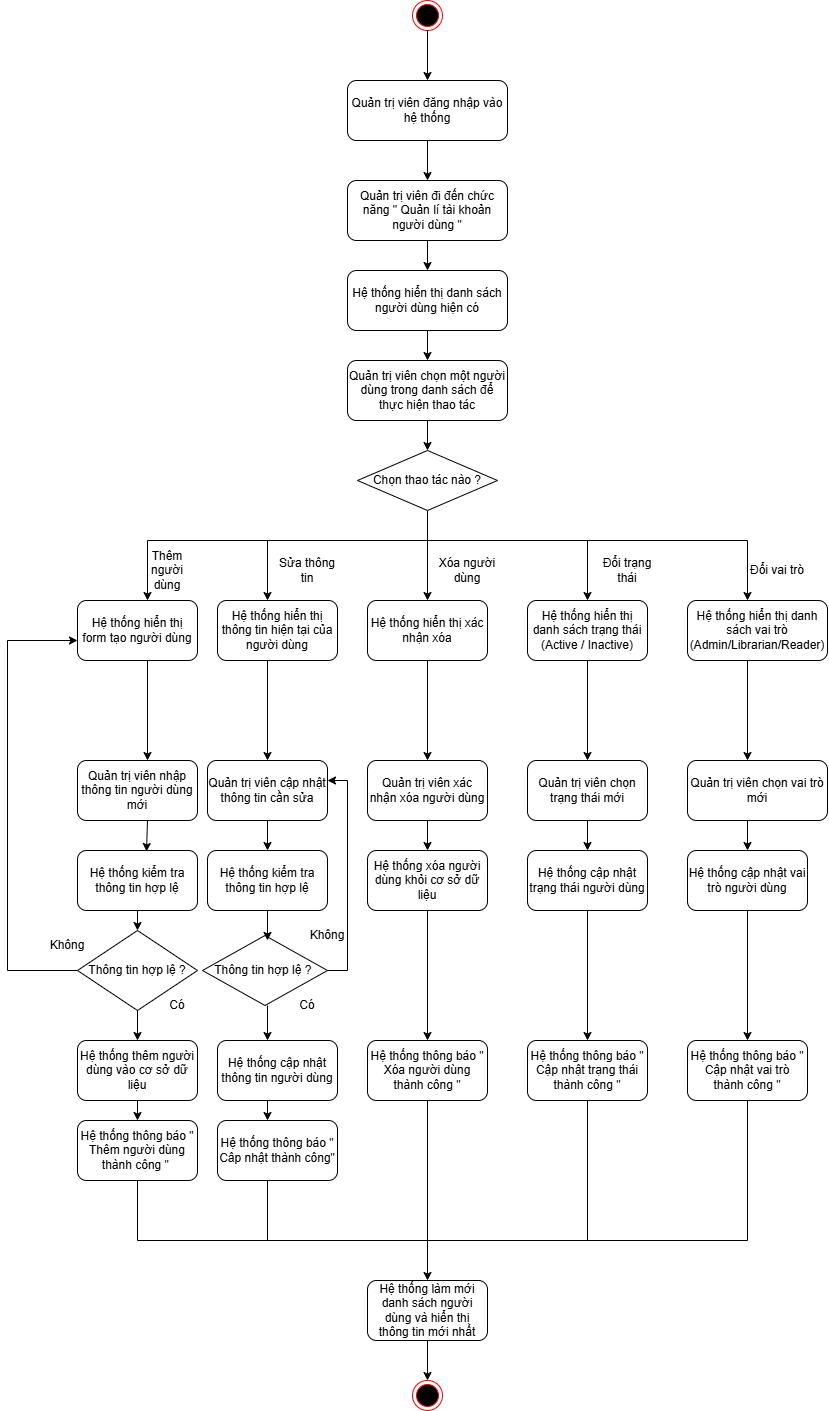
\includegraphics[width=0.6\linewidth]{Images/quanly.png}
    \vspace{10pt}
    \caption{Sơ đồ hoạt động Quản lý tài khoản người dùng}
    \label{fig:activity_manage_users}
\end{figure}

\begin{enumerate}
    \item Quản trị viên đăng nhập vào hệ thống.
    
    \item Quản trị viên truy cập chức năng ``Quản lý tài khoản người dùng''.
    
    \item Hệ thống hiển thị danh sách người dùng hiện có, bao gồm:
    \begin{itemize}
        \item ID.
        \item Họ tên.
        \item Email.
        \item Vai trò.
        \item Trạng thái.
    \end{itemize}
    
    \item Quản trị viên chọn một người dùng trong danh sách để thực hiện thao tác.
    
    \item Quản trị viên lựa chọn một trong các thao tác quản lý sau:
    \begin{itemize}
        \item Thêm người dùng.
        \item Sửa thông tin người dùng.
        \item Xóa người dùng.
        \item Đổi trạng thái tài khoản.
        \item Đổi vai trò người dùng.
    \end{itemize}

    \item \textbf{Trường hợp thêm người dùng}
    \begin{itemize}
        \item Hệ thống hiển thị form tạo người dùng.
        
        \item Quản trị viên nhập thông tin người dùng mới (họ tên, email, vai trò, \ldots).
        
        \item Hệ thống kiểm tra tính hợp lệ của dữ liệu.
        
        \item Nếu dữ liệu hợp lệ:
        \begin{itemize}
            \item Hệ thống thêm người dùng vào cơ sở dữ liệu.
            
            \item Hệ thống hiển thị thông báo ``Thêm người dùng thành công''.
        \end{itemize}
        
        \item Nếu dữ liệu không hợp lệ:
        \begin{itemize}
            \item Hệ thống hiển thị lỗi và yêu cầu nhập lại.
        \end{itemize}
    \end{itemize}

    \item \textbf{Trường hợp sửa thông tin người dùng}
    \begin{itemize}
        \item Hệ thống hiển thị thông tin hiện tại của người dùng.
        
        \item Quản trị viên cập nhật thông tin cần sửa.
        
        \item Hệ thống kiểm tra tính hợp lệ của dữ liệu.
        
        \item Nếu dữ liệu hợp lệ:
        \begin{itemize}
            \item Hệ thống cập nhật thông tin người dùng.
            
            \item Hệ thống hiển thị thông báo ``Cập nhật thành công''.
        \end{itemize}
        
        \item Nếu dữ liệu không hợp lệ:
        \begin{itemize}
            \item Hệ thống hiển thị lỗi và yêu cầu nhập lại.
        \end{itemize}
    \end{itemize}

    \item \textbf{Trường hợp xóa người dùng}
    \begin{itemize}
        \item Hệ thống hiển thị xác nhận xóa.
        
        \item Quản trị viên xác nhận xóa người dùng.
        
        \item Hệ thống xóa người dùng khỏi cơ sở dữ liệu.
        
        \item Hệ thống hiển thị thông báo ``Xóa người dùng thành công''.
    \end{itemize}

    \item \textbf{Trường hợp đổi trạng thái tài khoản}
    \begin{itemize}
        \item Hệ thống hiển thị danh sách trạng thái (Active/Inactive).
        
        \item Quản trị viên chọn trạng thái mới.
        
        \item Hệ thống cập nhật trạng thái người dùng.
        
        \item Hệ thống hiển thị thông báo ``Cập nhật trạng thái thành công''.
    \end{itemize}

    \item \textbf{Trường hợp đổi vai trò người dùng}
    \begin{itemize}
        \item Hệ thống hiển thị danh sách vai trò (Reader/Librarian/Admin/\ldots).
        
        \item Quản trị viên chọn vai trò mới.
        
        \item Hệ thống cập nhật vai trò người dùng.
        
        \item Hệ thống hiển thị thông báo ``Cập nhật vai trò thành công''.
    \end{itemize}

    \item Sau khi hoàn thành thao tác:
    \begin{itemize}
        \item Hệ thống làm mới danh sách người dùng.
        
        \item Hiển thị thông tin mới nhất.
    \end{itemize}
\end{enumerate}
\subsubsection{Thêm / Sửa / Xóa bản ghi tài liệu}

\begin{figure}[H]
    \centering
    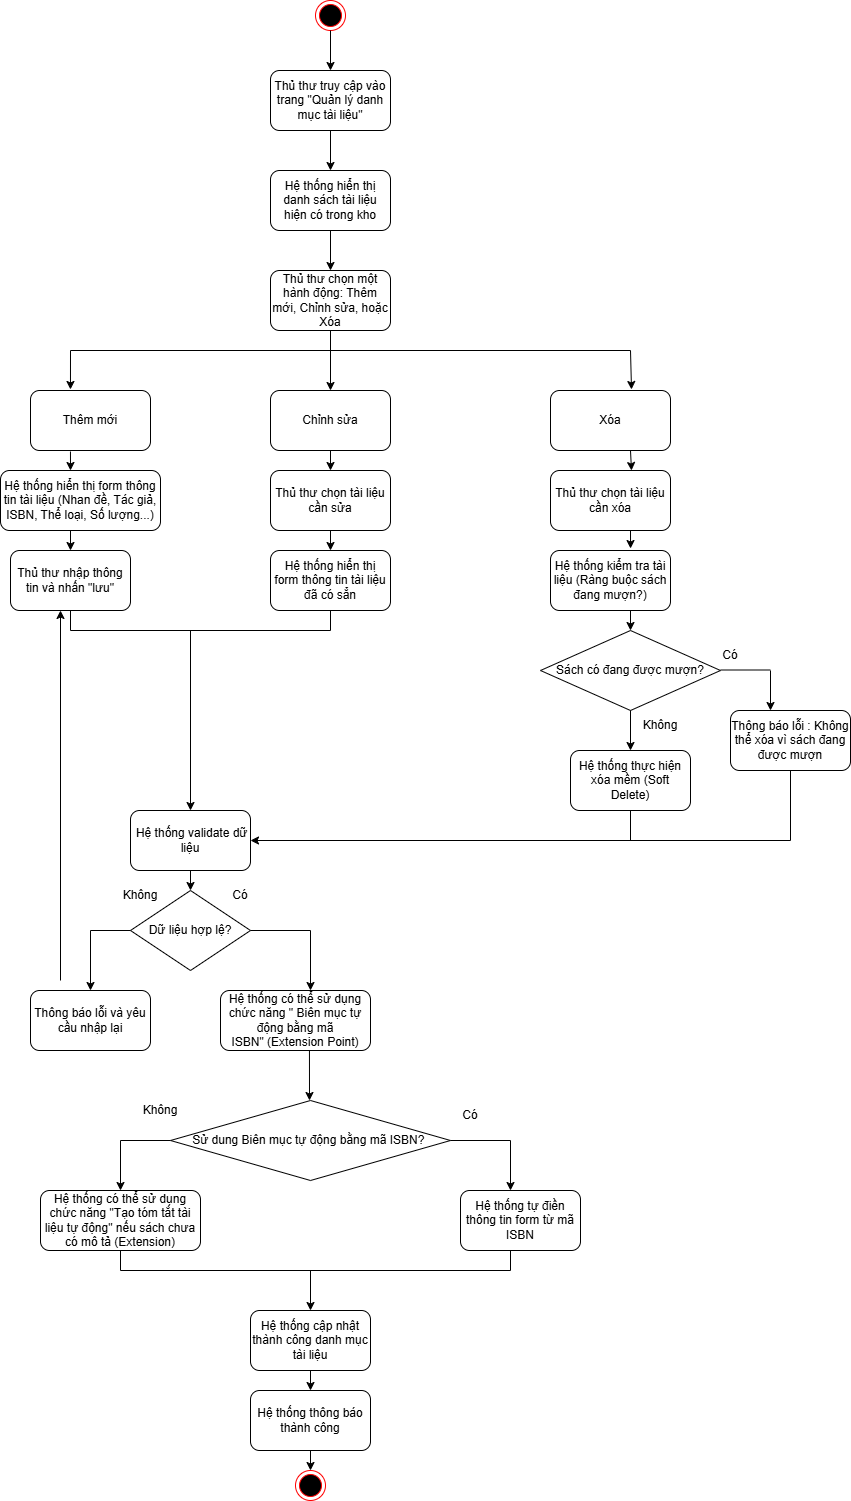
\includegraphics[width=0.6\linewidth]{Images/edit.png}
    \vspace{10pt}
    \caption{Sơ đồ hoạt động Thêm / Sửa / Xóa bản ghi tài liệu}
    \label{fig:activity_manage_documents}
\end{figure}

\begin{enumerate}
    \item Thủ thư truy cập trang ``Quản lý danh mục tài liệu''.
    
    \item Hệ thống hiển thị danh sách tài liệu hiện có trong kho.
    
    \item Thủ thư chọn một hành động:
    \begin{itemize}
        \item Thêm mới tài liệu.
        \item Chỉnh sửa tài liệu.
        \item Xóa tài liệu.
    \end{itemize}

    \item \textbf{Trường hợp thêm mới tài liệu}
    \begin{itemize}
        \item Hệ thống hiển thị biểu mẫu thông tin tài liệu:
        \begin{itemize}
            \item Nhan đề.
            \item Tác giả.
            \item ISBN.
            \item Thể loại.
            \item Số lượng.
            \item \ldots
        \end{itemize}
        
        \item Thủ thư nhập thông tin và nhấn ``Lưu''.
    \end{itemize}

    \item \textbf{Trường hợp chỉnh sửa tài liệu}
    \begin{itemize}
        \item Thủ thư chọn tài liệu cần sửa.
        
        \item Hệ thống hiển thị biểu mẫu chứa thông tin tài liệu đã có sẵn.
        
        \item Thủ thư cập nhật thông tin cần chỉnh sửa.
    \end{itemize}

    \item \textbf{Trường hợp xóa tài liệu}
    \begin{itemize}
        \item Thủ thư chọn tài liệu cần xóa.
        
        \item Hệ thống kiểm tra tài liệu có đang được mượn hay không.
        
        \item Nếu tài liệu đang được mượn:
        \begin{itemize}
            \item Hệ thống hiển thị thông báo lỗi:
            
            ``Không thể xóa vì sách đang được mượn''.
        \end{itemize}
        
        \item Nếu tài liệu không đang được mượn:
        \begin{itemize}
            \item Hệ thống thực hiện xóa mềm (Soft Delete).
        \end{itemize}
    \end{itemize}

    \item Hệ thống thực hiện validate dữ liệu.

    \item Nếu dữ liệu không hợp lệ:
    \begin{itemize}
        \item Hệ thống hiển thị thông báo lỗi.
        
        \item Yêu cầu thủ thư nhập lại thông tin.
    \end{itemize}

    \item Nếu dữ liệu hợp lệ:
    \begin{itemize}
        \item Hệ thống có thể sử dụng chức năng ``Biên mục tự động bằng mã ISBN'' (UC-CAT-03).
    \end{itemize}

    \item Nếu sử dụng biên mục tự động bằng ISBN:
    \begin{itemize}
        \item Hệ thống tự động điền thông tin tài liệu từ mã ISBN.
    \end{itemize}

    \item Nếu không sử dụng ISBN:
    \begin{itemize}
        \item Hệ thống có thể sử dụng chức năng ``Tạo tóm tắt tài liệu tự động'' (UC-CAT-04) nếu sách chưa có mô tả.
    \end{itemize}

    \item Hệ thống cập nhật thành công danh mục tài liệu.

    \item Hệ thống hiển thị thông báo thành công.
\end{enumerate}

\subsubsection{Nhập danh mục tài liệu hàng loạt}
\begin{figure}[H]
    \centering
    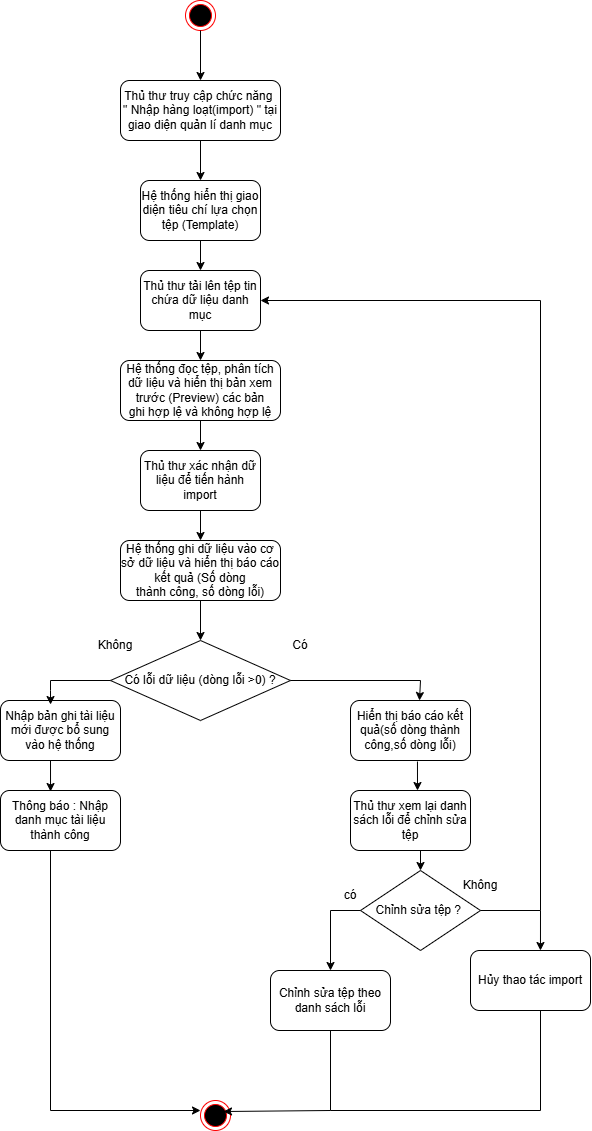
\includegraphics[width=0.6\linewidth]{Images/nhap.png}
    \vspace{10pt}
    \caption{Sơ đồ hoạt động Nhập danh mục tài liệu hàng loạt}
    \label{fig:activity_import}
\end{figure}

\begin{enumerate}
    \item Thủ thư truy cập chức năng ``Nhập hàng loạt (Import)'' tại giao diện quản lý danh mục.
    
    \item Hệ thống hiển thị giao diện tiêu chí lựa chọn tệp (Template).
    
    \item Thủ thư tải lên tệp tin chứa dữ liệu danh mục.
    
    \item Hệ thống đọc tệp, phân tích dữ liệu và hiển thị bản xem trước (Preview) các bản ghi hợp lệ và không hợp lệ.
    
    \item Thủ thư xác nhận dữ liệu để tiến hành import.
    
    \item Hệ thống ghi dữ liệu vào cơ sở dữ liệu và hiển thị báo cáo kết quả (Số dòng thành công, số dòng lỗi).
    
    \item Hệ thống kiểm tra: Có lỗi dữ liệu (dòng lỗi > 0) hay không?

    \item \textbf{Trường hợp Không có lỗi dữ liệu}
    \begin{itemize}
        \item Nhập bản ghi tài liệu mới được bổ sung vào hệ thống.
        
        \item Hệ thống hiển thị thông báo: 
        
        ``Nhập danh mục tài liệu thành công''.
        
        \item Kết thúc luồng hoạt động.
    \end{itemize}

    \item \textbf{Trường hợp Có lỗi dữ liệu}
    \begin{itemize}
        \item Hệ thống hiển thị báo cáo kết quả (Số dòng thành công, số dòng lỗi).
        
        \item Thủ thư xem lại danh sách lỗi để chỉnh sửa tệp.
        
        \item Hệ thống chờ quyết định: Có chỉnh sửa tệp hay không?
        
        \item \textbf{Nếu Có chỉnh sửa tệp:}
        \begin{itemize}
            \item Thủ thư tiến hành chỉnh sửa tệp theo danh sách lỗi.
            
            \item Quay lại bước: Thủ thư tải lên tệp tin chứa dữ liệu danh mục (Lặp lại quy trình).
        \end{itemize}
        
        \item \textbf{Nếu Không chỉnh sửa tệp:}
        \begin{itemize}
            \item Hệ thống thực hiện Hủy thao tác import.
            
            \item Kết thúc luồng hoạt động.
        \end{itemize}
    \end{itemize}
\end{enumerate}

\subsubsection{Biên mục tự động bằng mã ISBN}

\begin{figure}[H]
    \centering
    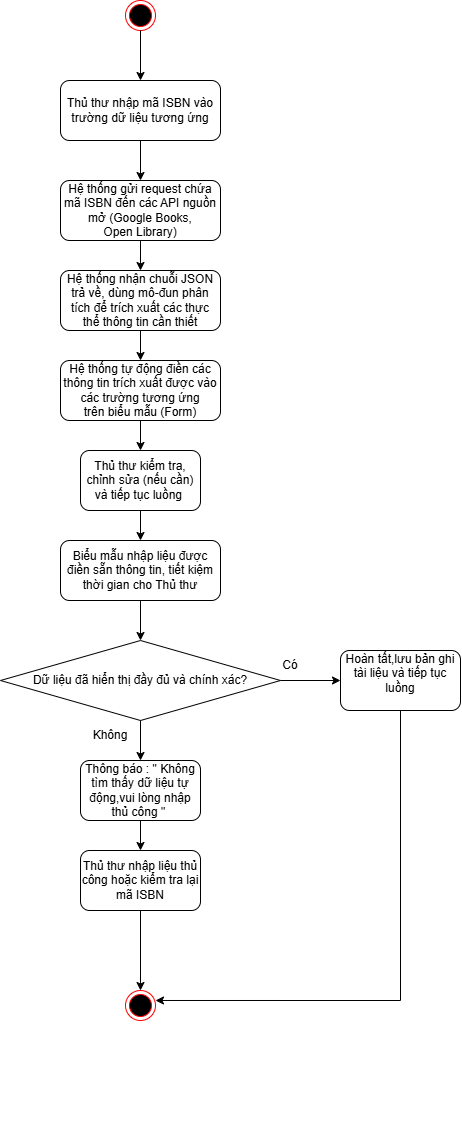
\includegraphics[width=0.6\linewidth]{Images/bienmuc.png}
    \vspace{10pt}
    \caption{Sơ đồ hoạt động Biên mục tự động bằng mã ISBN}
    \label{fig:activity_isbn}
\end{figure}
\begin{enumerate}
    \item Thủ thư nhập mã ISBN vào trường dữ liệu tương ứng.
    
    \item Hệ thống gửi request chứa mã ISBN đến các API nguồn mở (Google Books, Open Library).
    
    \item Hệ thống nhận chuỗi JSON trả về, dùng mô-đun phân tích để trích xuất các thực thể thông tin cần thiết.
    
    \item Hệ thống tự động điền các thông tin trích xuất được vào các trường tương ứng trên biểu mẫu (Form).
    
    \item Thủ thư kiểm tra, chỉnh sửa (nếu cần) và tiếp tục luồng của  ``Thêm / Sửa / Xóa bản ghi tài liệu''.
    
    \item Biểu mẫu nhập liệu được điền sẵn thông tin, tiết kiệm thời gian cho Thủ thư.

    \item Hệ thống kiểm tra: Dữ liệu đã hiển thị đầy đủ và chính xác?

    \item \textbf{Trường hợp dữ liệu đầy đủ và chính xác (Có)}
    \begin{itemize}
        \item Hoàn tất, lưu bản ghi tài liệu và tiếp tục luồng.
        \item Kết thúc luồng hoạt động.
    \end{itemize}

    \item \textbf{Trường hợp dữ liệu không đầy đủ hoặc không chính xác (Không)}
    \begin{itemize}
        \item Hệ thống hiển thị thông báo: 
        
        ``Không tìm thấy dữ liệu tự động, vui lòng nhập thủ công''.
        
        \item Thủ thư thực hiện nhập liệu thủ công hoặc kiểm tra lại mã ISBN.
        
        \item Kết thúc luồng hoạt động.
    \end{itemize}
\end{enumerate}

\subsubsection{Mượn tài liệu vật lý}
\begin{figure}[H]
    \centering
    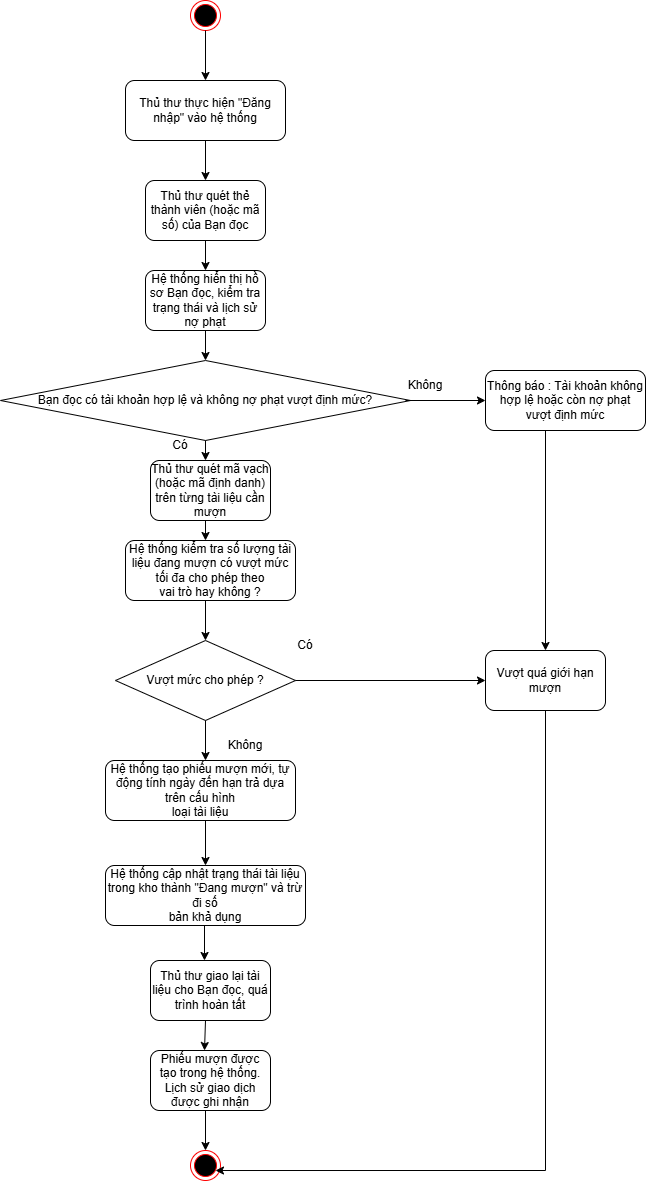
\includegraphics[width=0.6\linewidth]{Images/muon.png}
    \vspace{10pt}
    \caption{Sơ đồ hoạt động  Mượn tài liệu vật lý}
    \label{fig:activity_borrow}
\end{figure}

\begin{enumerate}
    \item Thủ thư thực hiện ``Đăng nhập'' vào hệ thống.
    
    \item Thủ thư quét thẻ thành viên (hoặc mã số) của Bạn đọc.
    
    \item Hệ thống hiển thị hồ sơ Bạn đọc, kiểm tra trạng thái và lịch sử nợ phạt.
    
    \item Hệ thống kiểm tra điều kiện: Bạn đọc có tài khoản hợp lệ và không nợ phạt vượt định mức?

    \item \textbf{Trường hợp không đủ điều kiện (Không)}
    \begin{itemize}
        \item Hệ thống hiển thị thông báo: 
        
        ``Tài khoản không hợp lệ hoặc còn nợ phạt vượt định mức''.
        
        \item Kết thúc luồng hoạt động.
    \end{itemize}

    \item \textbf{Trường hợp đủ điều kiện (Có)}
    \begin{itemize}
        \item Thủ thư quét mã vạch (hoặc mã định danh) trên từng tài liệu cần mượn.
        
        \item Hệ thống kiểm tra số lượng tài liệu đang mượn có vượt mức tối đa cho phép theo vai trò hay không.
    \end{itemize}

    \item Hệ thống kiểm tra điều kiện: Vượt mức cho phép?

    \item \textbf{Trường hợp Vượt mức cho phép (Có)}
    \begin{itemize}
        \item Hệ thống hiển thị thông báo: ``Vượt quá giới hạn mượn''.
        
        \item Kết thúc luồng hoạt động.
    \end{itemize}

    \item \textbf{Trường hợp Không vượt mức cho phép (Không)}
    \begin{itemize}
        \item Hệ thống tạo phiếu mượn mới, tự động tính ngày đến hạn trả dựa trên cấu hình loại tài liệu.
        
        \item Hệ thống cập nhật trạng thái tài liệu trong kho thành ``Đang mượn'' và trừ đi số bản khả dụng.
        
        \item Thủ thư giao lại tài liệu cho Bạn đọc, quá trình hoàn tất.
        
        \item Phiếu mượn được tạo trong hệ thống, lịch sử giao dịch được ghi nhận.
        
        \item Kết thúc luồng hoạt động.
    \end{itemize}
\end{enumerate}

\subsubsection{Trả tài liệu}
\begin{figure}[H]
    \centering
    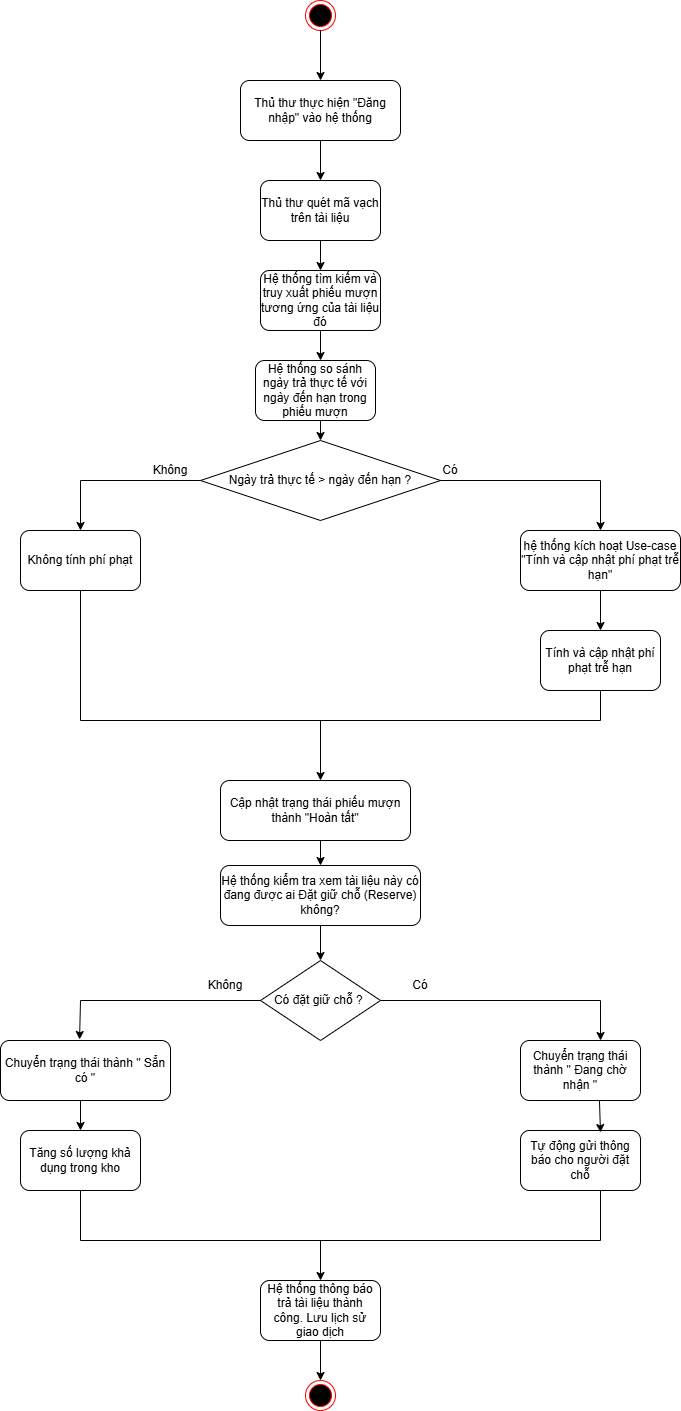
\includegraphics[width=0.6\linewidth]{Images/tra.png}
    \vspace{10pt}
    \caption{Sơ đồ hoạt động Trả tài liệu}
    \label{fig:activity_return}
\end{figure}
\begin{enumerate}
    \item Thủ thư thực hiện ``Đăng nhập'' vào hệ thống.
    
    \item Thủ thư quét mã vạch trên tài liệu.
    
    \item Hệ thống tìm kiếm và truy xuất phiếu mượn tương ứng của tài liệu đó.
    
    \item Hệ thống so sánh ngày trả thực tế với ngày đến hạn trong phiếu mượn.
    
    \item Hệ thống kiểm tra điều kiện: Ngày trả thực tế $>$ ngày đến hạn?

    \item \textbf{Trường hợp Trả trễ hạn (Có)}
    \begin{itemize}
        \item Hệ thống kích hoạt  ``Tính và cập nhật phí phạt trễ hạn'' .
        
        \item Tính và cập nhật phí phạt trễ hạn.
    \end{itemize}

    \item \textbf{Trường hợp Trả đúng hạn (Không)}
    \begin{itemize}
        \item Hệ thống không tính phí phạt.
    \end{itemize}

    \item Cập nhật trạng thái phiếu mượn thành ``Hoàn tất''.

    \item Hệ thống kiểm tra xem tài liệu này có đang được ai Đặt giữ chỗ (Reserve) không?

    \item \textbf{Trường hợp Có Đặt giữ chỗ (Có)}
    \begin{itemize}
        \item Chuyển trạng thái tài liệu thành ``Đang chờ nhận''.
        
        \item Tự động gửi thông báo cho người đặt chỗ.
    \end{itemize}

    \item \textbf{Trường hợp Không có Đặt giữ chỗ (Không)}
    \begin{itemize}
        \item Chuyển trạng thái tài liệu thành ``Sẵn có''.
        
        \item Tăng số lượng khả dụng trong kho.
    \end{itemize}

    \item Hiển thị thông báo trả tài liệu thành công và lưu lịch sử giao dịch.

    \item Kết thúc luồng hoạt động.
\end{enumerate}

\subsubsection{Tính và cập nhật phí phạt trễ hạn}
\begin{figure}[H]
    \centering
    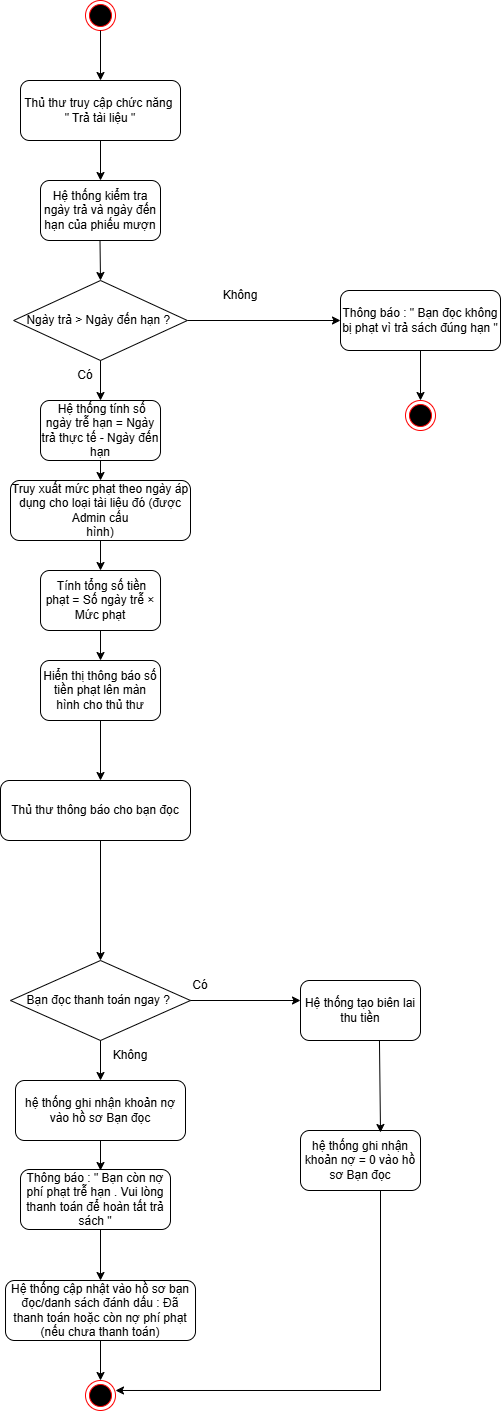
\includegraphics[width=0.6\linewidth]{Images/phiphat.png}
    \vspace{10pt}
    \caption{Sơ đồ hoạt động Tính và cập nhật phí phạt trễ hạn}
    \label{fig:activity_fine}
\end{figure}

\begin{enumerate}
    \item Thủ thư truy cập chức năng ``Trả tài liệu''.
    
    \item Hệ thống kiểm tra ngày hệ thống (ngày trả) và ngày đến hạn của phiếu mượn.
    
    \item Hệ thống kiểm tra điều kiện: Ngày trả $>$ Ngày đến hạn?

    \item \textbf{Trường hợp trả sách đúng hạn (Không)}
    \begin{itemize}
        \item Hệ thống hiển thị thông báo: ``Bạn đọc không bị phạt vì trả sách đúng hạn''.
        \item Kết thúc luồng hoạt động.
    \end{itemize}

    \item \textbf{Trường hợp trả sách trễ hạn (Có)}
    \begin{itemize}
        \item Hệ thống tính số ngày trễ hạn = Ngày trả thực tế - Ngày đến hạn.
        
        \item Hệ thống truy xuất mức phạt theo ngày áp dụng cho loại tài liệu đó .
        
        \item Hệ thống tính tổng số tiền phạt = Số ngày trễ $\times$ Mức phạt.
        
        \item Hệ thống hiển thị thông báo số tiền phạt lên màn hình cho thủ thư.
        
        \item Thủ thư thông báo cho bạn đọc.
    \end{itemize}

    \item Hệ thống kiểm tra: Bạn đọc thanh toán ngay?

    \item \textbf{Trường hợp thanh toán ngay (Có)}
    \begin{itemize}
        \item Hệ thống tạo biên lai thu tiền.
        \item Hệ thống ghi nhận khoản nợ = 0 vào hồ sơ bạn đọc.
    \end{itemize}

    \item \textbf{Trường hợp chưa thanh toán ngay (Không)}
    \begin{itemize}
        \item Hệ thống ghi nhận khoản nợ vào hồ sơ bạn đọc.
        \item Hệ thống hiển thị thông báo: ``Bạn còn nợ phí phạt trễ hạn. Vui lòng thanh toán để hoàn tất trả sách.''
    \end{itemize}

    \item Hệ thống cập nhật vào hồ sơ bạn đọc/ danh sách đánh dấu: Đã thanh toán hoặc Còn nợ phí phạt (nếu chưa thanh toán).

    \item Kết thúc luồng hoạt động.

   
\end{enumerate}

\subsubsection{Gia hạn tài liệu trực tuyến}
\begin{figure}[H]
    \centering
    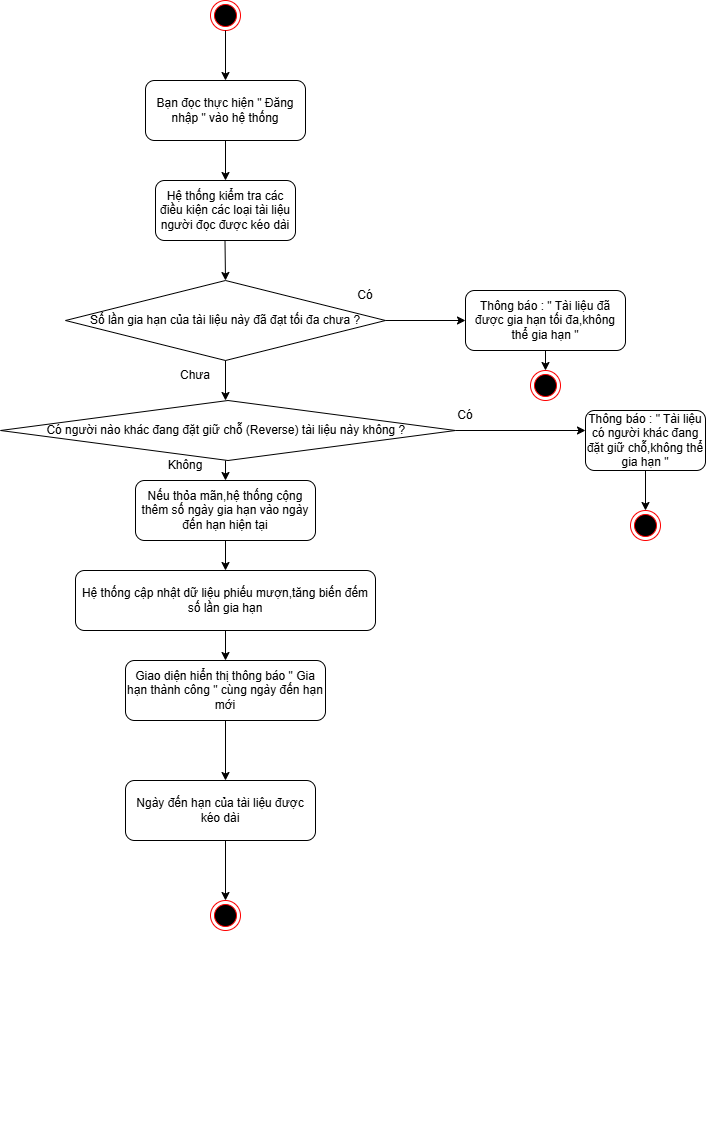
\includegraphics[width=0.6\linewidth]{Images/giahan.png}
    \vspace{10pt}
    \caption{Sơ đồ hoạt động Gia hạn tài liệu trực tuyến}
    \label{fig:activity_extend}
\end{figure}

\begin{enumerate}
    \item Bạn đọc thực hiện ``Đăng nhập'' vào hệ thống.
    
    \item Hệ thống kiểm tra và điều kiện các loại tài liệu người đọc được kéo dài.
    
    \item Hệ thống kiểm tra: Số lần gia hạn của tài liệu này đã đạt tối đa chưa?

    \item \textbf{Trường hợp đã đạt số lần gia hạn tối đa (Có)}
    \begin{itemize}
        \item Hệ thống hiển thị thông báo: ``Tài liệu đã được gia hạn tối đa, không thể gia hạn''.
        \item Kết thúc luồng hoạt động.
    \end{itemize}

    \item \textbf{Trường hợp chưa đạt số lần gia hạn tối đa (Chưa)}
    \begin{itemize}
        \item Hệ thống kiểm tra: Có người đang nào khác đang đặt giữ chỗ (Reserve) tài liệu này không?
    \end{itemize}

    \item \textbf{Trường hợp có người khác đang đặt giữ chỗ (Có)}
    \begin{itemize}
        \item Hệ thống hiển thị thông báo: ``Tài liệu có người khác đang đặt giữ chỗ, không thể gia hạn''.
        \item Kết thúc luồng hoạt động.
    \end{itemize}

    \item \textbf{Trường hợp không có người đặt giữ chỗ (Không)}
    \begin{itemize}
        \item Nếu thỏa mãn, hệ thống cộng thêm số ngày gia hạn vào ngày đến hạn hiện tại.
        
        \item Hệ thống cập nhật dữ liệu phiếu mượn, tăng biến đếm số lần gia hạn.
        
        \item Giao diện hiển thị thông báo ``Gia hạn thành công'' cùng ngày đến hạn mới.
        
        \item Ngày đến hạn của tài liệu được kéo dài.
        
        \item Kết thúc luồng hoạt động.
    \end{itemize}

\end{enumerate}

\subsubsection{Đặt giữ chỗ tài liệu}
\begin{figure}[H]
    \centering
    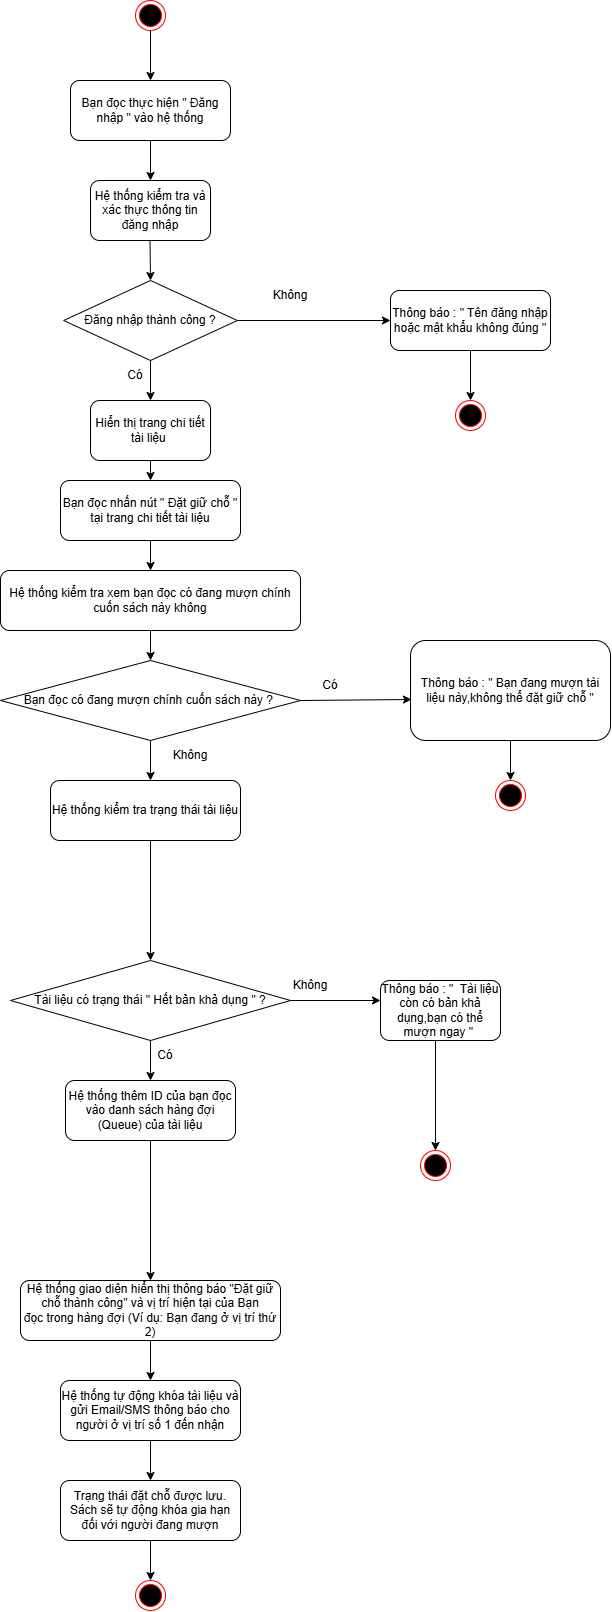
\includegraphics[width=0.6\linewidth]{Images/dat.png}
    \vspace{10pt}
    \caption{Sơ đồ hoạt động Đặt giữ chỗ tài liệu}
    \label{fig:activity_reserve}
\end{figure}

\begin{enumerate}
    \item Bạn đọc thực hiện ``Đăng nhập'' vào hệ thống.
    
    \item Hệ thống kiểm tra và xác thực thông tin đăng nhập.
    
    \item Hệ thống kiểm tra: Đăng nhập thành công?

    \item \textbf{Trường hợp đăng nhập thất bại (Không)}
    \begin{itemize}
        \item Hệ thống hiển thị thông báo: ``Tên đăng nhập hoặc mật khẩu không đúng''.
        \item Kết thúc luồng hoạt động.
    \end{itemize}

    \item \textbf{Trường hợp đăng nhập thành công (Có)}
    \begin{itemize}
        \item Hệ thống hiển thị trang chi tiết tài liệu.
        \item Bạn đọc nhấn nút ``Đặt giữ chỗ'' tại trang chi tiết tài liệu.
        \item Hệ thống kiểm tra xem bạn đọc có đang mượn chính cuốn sách này không.
    \end{itemize}

    \item Hệ thống kiểm tra: Bạn đọc có đang mượn chính cuốn sách này?

    \item \textbf{Trường hợp đang mượn sách này (Có)}
    \begin{itemize}
        \item Hệ thống hiển thị thông báo: ``Bạn đang mượn tài liệu này, không thể đặt giữ chỗ''.
        \item Kết thúc luồng hoạt động.
    \end{itemize}

    \item \textbf{Trường hợp không mượn sách này (Không)}
    \begin{itemize}
        \item Hệ thống kiểm tra trạng thái tài liệu.
    \end{itemize}

    \item Hệ thống kiểm tra: Tài liệu có trạng thái ``Hết bản khả dụng''?

    \item \textbf{Trường hợp tài liệu vẫn còn bản khả dụng (Không)}
    \begin{itemize}
        \item Hệ thống hiển thị thông báo: ``Tài liệu còn bản khả dụng, bạn có thể mượn ngay''.
        \item Kết thúc luồng hoạt động.
    \end{itemize}

    \item \textbf{Trường hợp tài liệu đã hết bản khả dụng (Có)}
    \begin{itemize}
        \item Hệ thống thêm ID của bạn đọc vào danh sách hàng đợi (Queue) của tài liệu.
        \item Giao diện hiển thị thông báo ``Đặt giữ chỗ thành công'' và vị trí hiện tại của bạn đọc trong hàng đợi (Ví dụ: Bạn đang ở vị trí thứ 2).
        \item Hệ thống tự động khóa tài liệu và gửi Email/SMS thông báo cho người ở vị trí số 1 đến nhận.
        \item Trạng thái đặt chỗ được lưu. Sách sẽ tự động khóa gia hạn đối với người đang mượn.
        \item Kết thúc luồng hoạt động.
    \end{itemize}

    
\end{enumerate}

\subsubsection{Tra cứu tài liệu}
\begin{figure}[H]
    \centering
    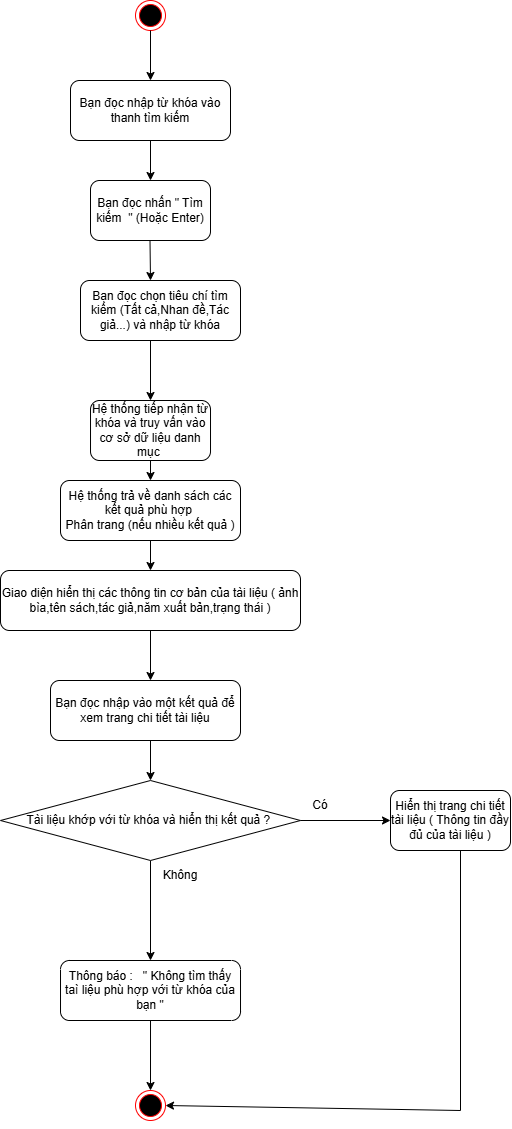
\includegraphics[width=0.6\linewidth]{Images/tracuu.png}
    \vspace{10pt}
    \caption{Sơ đồ hoạt động Tra cứu tài liệu}
    \label{fig:activity_search}
\end{figure}
\begin{enumerate}
    \item Bạn đọc nhập từ khóa vào thanh tìm kiếm.
    
    \item Bạn đọc nhấn ``Tìm kiếm'' (hoặc nhấn Enter).
    
    \item Bạn đọc chọn tiêu chí tìm kiếm (Tất cả, Nhan đề, Tác giả\ldots) và nhập từ khóa.
    
    \item Hệ thống tiếp nhận từ khóa và truy vấn vào cơ sở dữ liệu danh mục.
    
    \item Hệ thống trả về danh sách các kết quả phù hợp, thực hiện phân trang (nếu có nhiều kết quả).
    
    \item Giao diện hiển thị các thông tin cơ bản của tài liệu bao gồm:
    \begin{itemize}
        \item Ảnh bìa.
        \item Tên sách.
        \item Tác giả.
        \item Năm xuất bản.
        \item Trạng thái (Còn bản vật lý / Có bản Digital).
    \end{itemize}

    \item Bạn đọc nhấp vào một kết quả để xem trang chi tiết tài liệu.

    \item Hệ thống kiểm tra điều kiện: Tài liệu khớp với từ khóa và hiển thị kết quả?

    \item \textbf{Trường hợp tìm thấy kết quả (Có)}
    \begin{itemize}
        \item Hệ thống hiển thị trang chi tiết tài liệu (thông tin đầy đủ của tài liệu).
        \item Kết thúc luồng hoạt động.
    \end{itemize}

    \item \textbf{Trường hợp không tìm thấy kết quả (Không)}
    \begin{itemize}
        \item Hệ thống hiển thị thông báo: 
        
        ``Không tìm thấy tài liệu phù hợp với từ khóa của bạn''.
        
        \item Kết thúc luồng hoạt động.
    \end{itemize}

   
\end{enumerate}
\subsection{Sơ đồ tuần tự (Sequence Diagram)}
\subsubsection{Đăng kí tài khoản}
\begin{figure}[H]
    \centering
    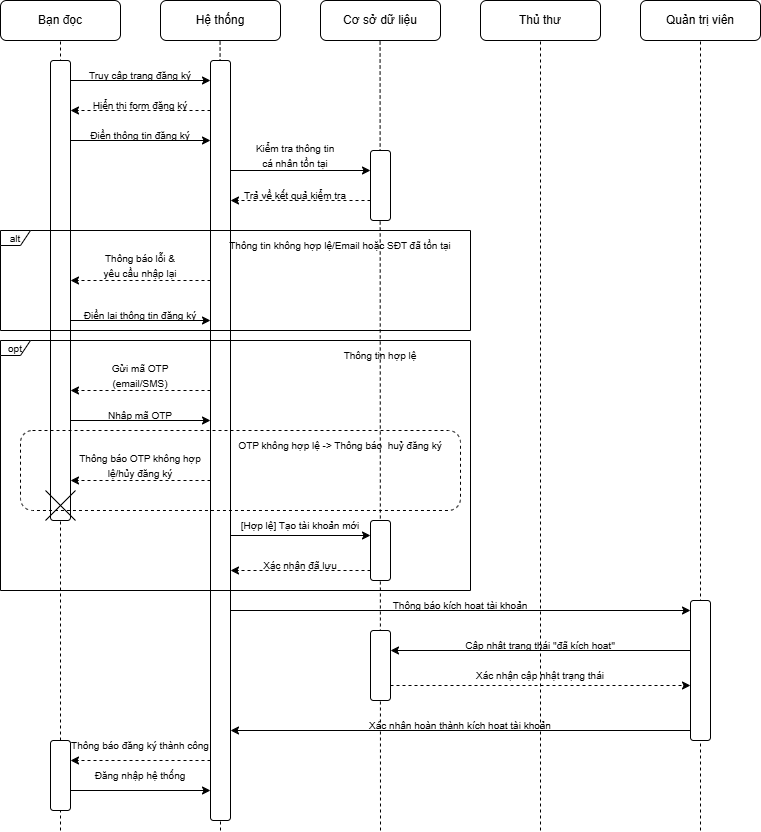
\includegraphics[width=0.6\linewidth]{Images/Seq_Dang ky.png}
    \vspace{10pt}
    \caption{Sơ đồ tuần tự Đăng kí tài khoản}
    \label{fig:sequence_register}
\end{figure}
\begin{enumerate}
    \item Bạn đọc tiến hành truy cập trang đăng kí tài khoản, hệ thống hiển thị giao diện tương ứng.
    \item Bạn đọc tiến hành điền thông tin đăng ký để hệ thống kiểm tra tính hợp lệ và không trùng lặp với thông tin hiện có trong cơ sở dữ liệu.
    \item \textbf{Khi thông tin không hợp lệ:}
    \begin{itemize}
        \item Hệ thống báo lỗi và yêu cầu bạn đọc nhập lại thông tin.
        \item Bạn đọc tiến hành nhập lại thông tin từ bước 2.
    \end{itemize}
    \item Khi thông tin được xác minh hợp lệ, mã OTP được gửi đến bạn đọc thông qua hệ thống email và yêu cầu bạn đọc nhập mã OTP.
    \item Nếu mã OTP\textbf{ không hợp lệ}, hệ thống thông báo mã OTP không trùng khớp, \textbf{hủy quá trình đăng ký tài khoản} và quy trình kết thúc tại đây, nếu không thì tiến hành tạo tài khoản mới trong cơ sở dữ liệu.
    \item Sau khi tài khoản mới được tạo, Quản trị viên được thông báo kích hoạt tài khoản cho bạn đọc mới, sau đó Quản trị viên tiến hành kích hoạt, qua đó cập nhật trạng thái cho tài khoản bạn đọc mới và gửi thông báo "Tài khoản đăng ký thành công" cho bạn đọc mới, từ đó bạn đọc mới có thể sử dụng tài khoản để đăng nhập hệ thống và tiến hành truy cập kho tài liệu.
\end{enumerate}
\subsubsection{Đăng nhập tài khoản}
\begin{figure}[H]
    \centering
    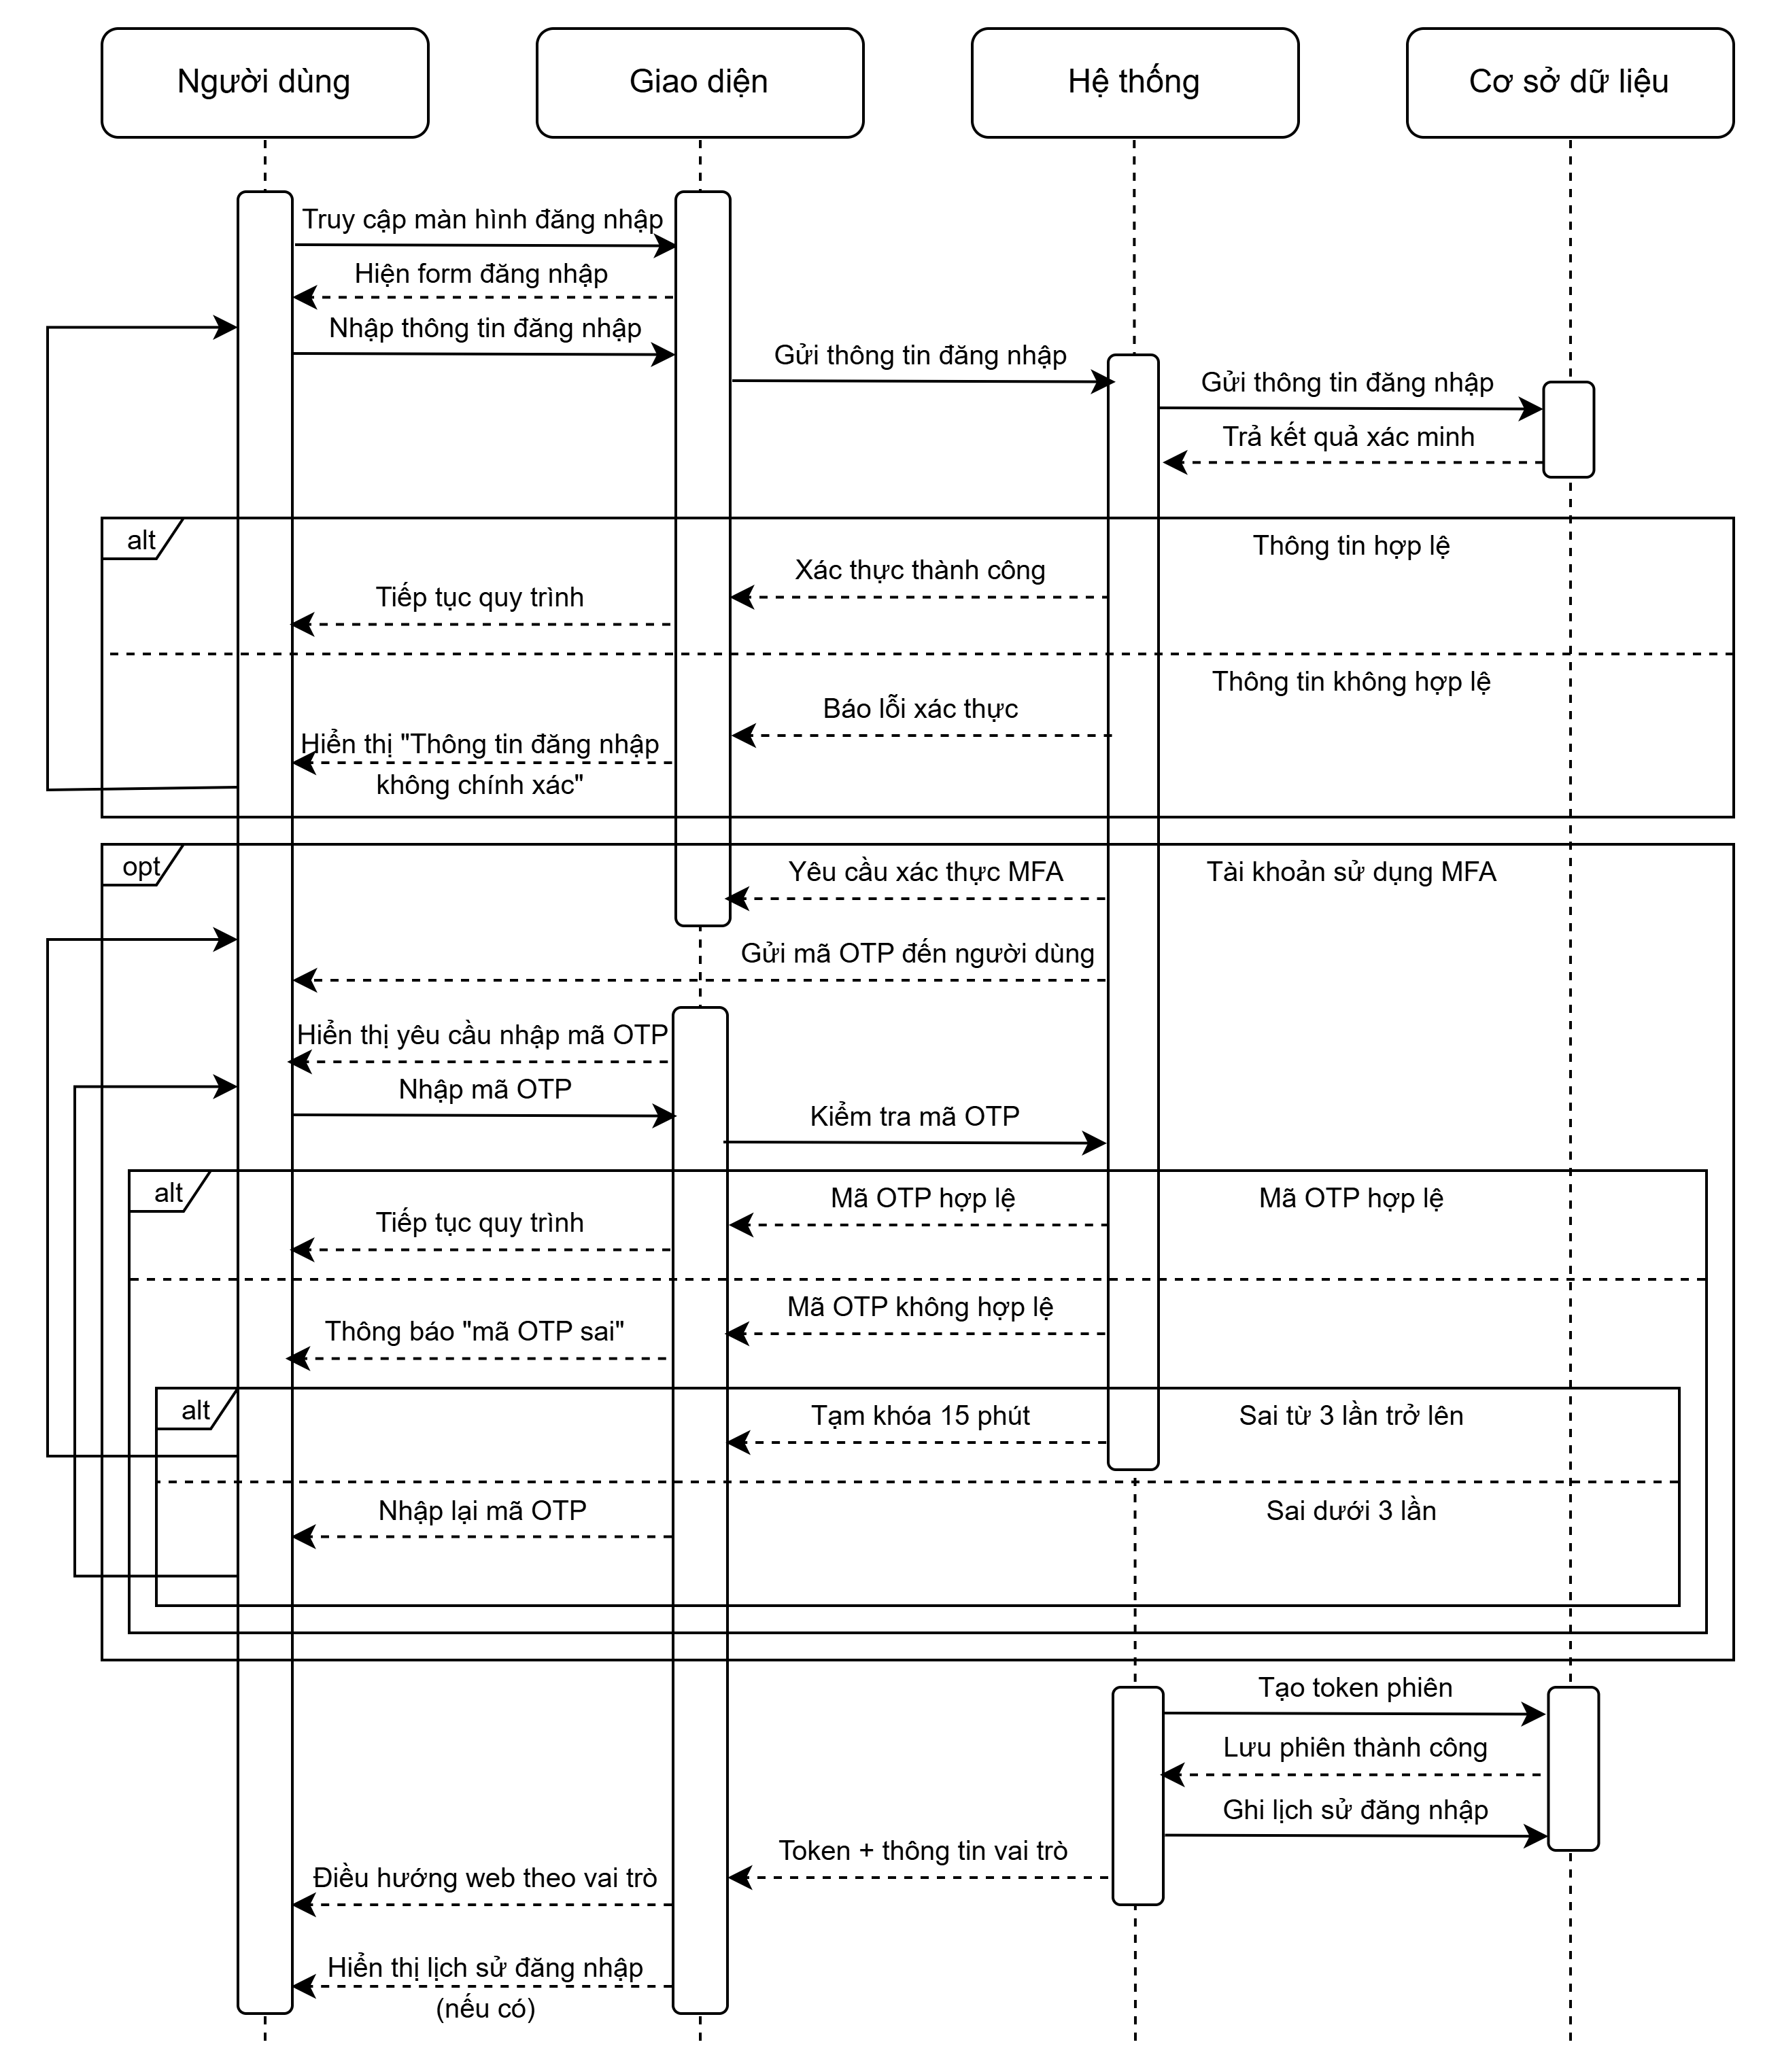
\includegraphics[width=0.6\linewidth]{Images/Seq_Dang nhap.png}
    \vspace{10pt}
    \caption{Sơ đồ tuần tự Đăng nhập tài khoản}
    \label{fig:sequence_login}
\end{figure}
\begin{enumerate}
    \item Người dùng tiến hành truy cập trang đăng nhập, hệ thống hiển thị giao diện đăng nhập.
    \item Sau khi người dùng điền thông tin đăng nhập, hệ thống sử dụng thông tin được cung cấp để đối chiếu với thông tin lưu trong cơ sở dữ liệu.
    \item Khi thông tin \textbf{không hợp lệ}, hệ thống báo lỗi "Thông tin đăng nhập không chính xác", yêu cầu người dùng điền lại thông tin, người dùng thực hiện lại từ bước 2. Nếu không, quy trình tiếp tục.
    \item Đối với các tài khoản sử dụng Xác thực đa yếu tố (MFA), hệ thống gửi yêu cầu xác thực bằng cách gửi mã OTP đến người dùng, đồng thời hiện giao diện xác thực bằng mã OTP. Nếu tài khoản \textbf{không sử dụng MFA}, người dùng bỏ qua bước này.
    \begin{itemize}
        \item Sau khi nhập mã xác thực OTP, nếu mã trùng khớp và hợp lệ, quy trình đăng nhập tiếp tục. Nếu không, hệ thống báo lỗi "Mã OTP sai".
        \item Trong quá trình nhập mã OTP, nếu nhập sai từ 3 lần trở lên, tài khoản khóa tạm thời trong 15 phút sau mỗi lần nhập sai mã OTP. Quá trình tạm khóa tài khoản chỉ dừng lại và cài lại bộ đếm nhập sai khi người dùng nhập chính xác mã OTP.
    \end{itemize}
    \item Sau khi thông tin xác thực thành công, token cho phiên đăng nhập được tạo và lưu tạm thời, đồng thời ghi lại lịch sử đăng nhập và gửi về hệ thống. Hệ thống điều hướng người dùng theo vai trò của tài khoản người dùng (Bạn đọc, Thủ thư hoặc Quản trị viên).
    \item Nếu có lịch sử đăng nhập, danh sách được hiển thị.
\end{enumerate}
\subsubsection{Đặt lại mật khẩu tài khoản}
\begin{figure}[H]
    \centering
    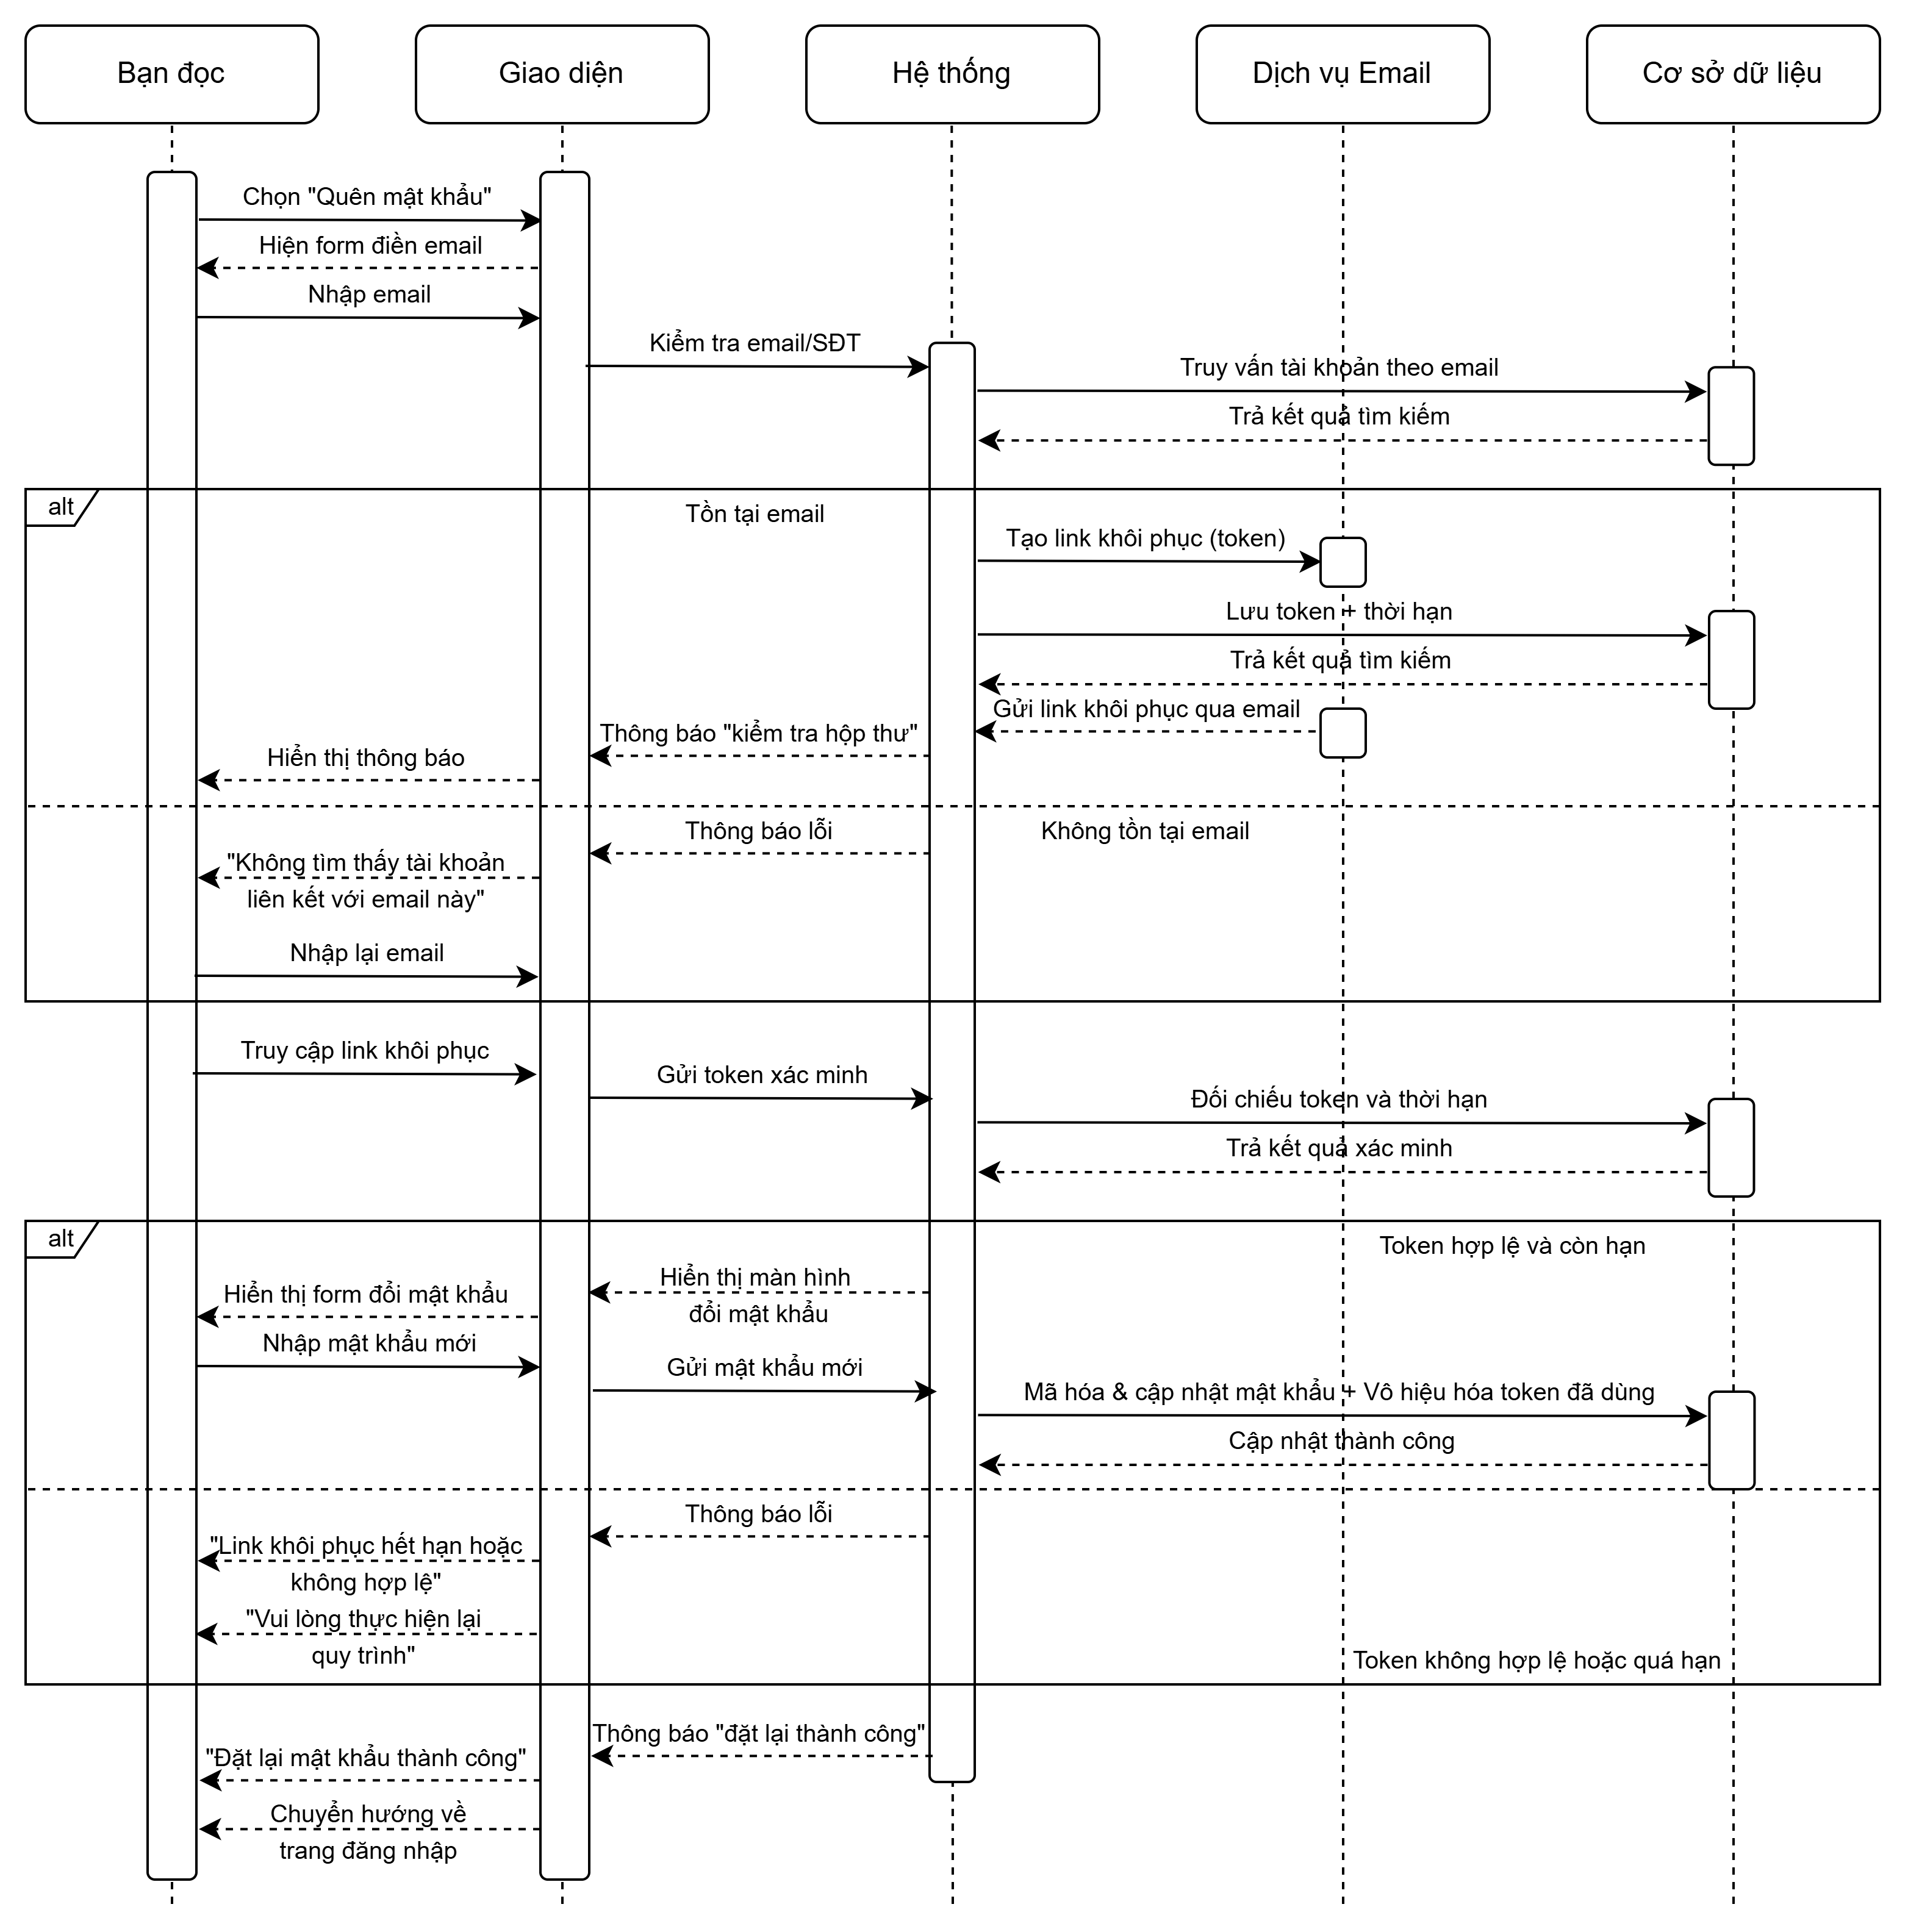
\includegraphics[width=0.6\linewidth]{Images/Seq_Reset mat khau.png}
    \vspace{10pt}
    \caption{Sơ đồ tuần tự Đặt lại mật khẩu tài khoản}
    \label{fig:sequence_reset_password}
\end{figure}
\begin{enumerate}
    \item Bạn đọc tiến hành chọn "Quên mật khẩu" ở trang đăng nhập, sau đó tiến hành nhập email gắn với tài khoản cần đặt lại mật khẩu.
    \item Hệ thống đối chiếu thông tin trong cơ sở dữ liệu để kiểm tra có tài khoản nào liên kết với email hay không.
    \item Nếu email \textbf{không được liên kết với bất kỳ tài khoản nào}:
    \begin{itemize}
        \item Hệ thống báo lỗi "Không tìm thấy tài khoản liên kết với email này".
        \item Bạn đọc tiến hành nhập lại email và hệ thống thực hiện kiểm tra lại (như bước 2).
        \item Quy trình tìm tài khoản liên kết với email chỉ dừng khi tìm được tài khoản liên kết với email tương ứng, hoặc người dùng thoát khỏi trang.
    \end{itemize}
    Nếu không, hệ thống tiến hành tạo link đặt lại mật khẩu (token) và lưu tạm thời cùng với hạn sử dụng, sau đó gửi link đặt lại mật khẩu cho người dùng qua dịch vụ email.
    \item Khi bạn đọc mở đường link đặt lại mật khẩu được gửi ở bước 3, hệ thống kiểm tra token và thời hạn sử dụng.
    \begin{itemize}
        \item Nếu token hợp lệ và chưa hết hạn, hệ thống điều hướng sang phần \textbf{Đặt lại mật khẩu}, người dùng thay đổi mật khẩu và hệ thống cập nhật sau khi hoàn thành.
        \item Nếu token không hợp lệ hoặc đã hết hạn, hệ thống thông báo "Link không hợp lệ hoặc đã hết hạn", quy trình \textbf{kết thúc tại đây}, người dùng thực hiện lại từ đầu.
    \end{itemize}
\end{enumerate}
\subsubsection{Tìm kiếm tài liệu}
\begin{figure}[H]
    \centering
    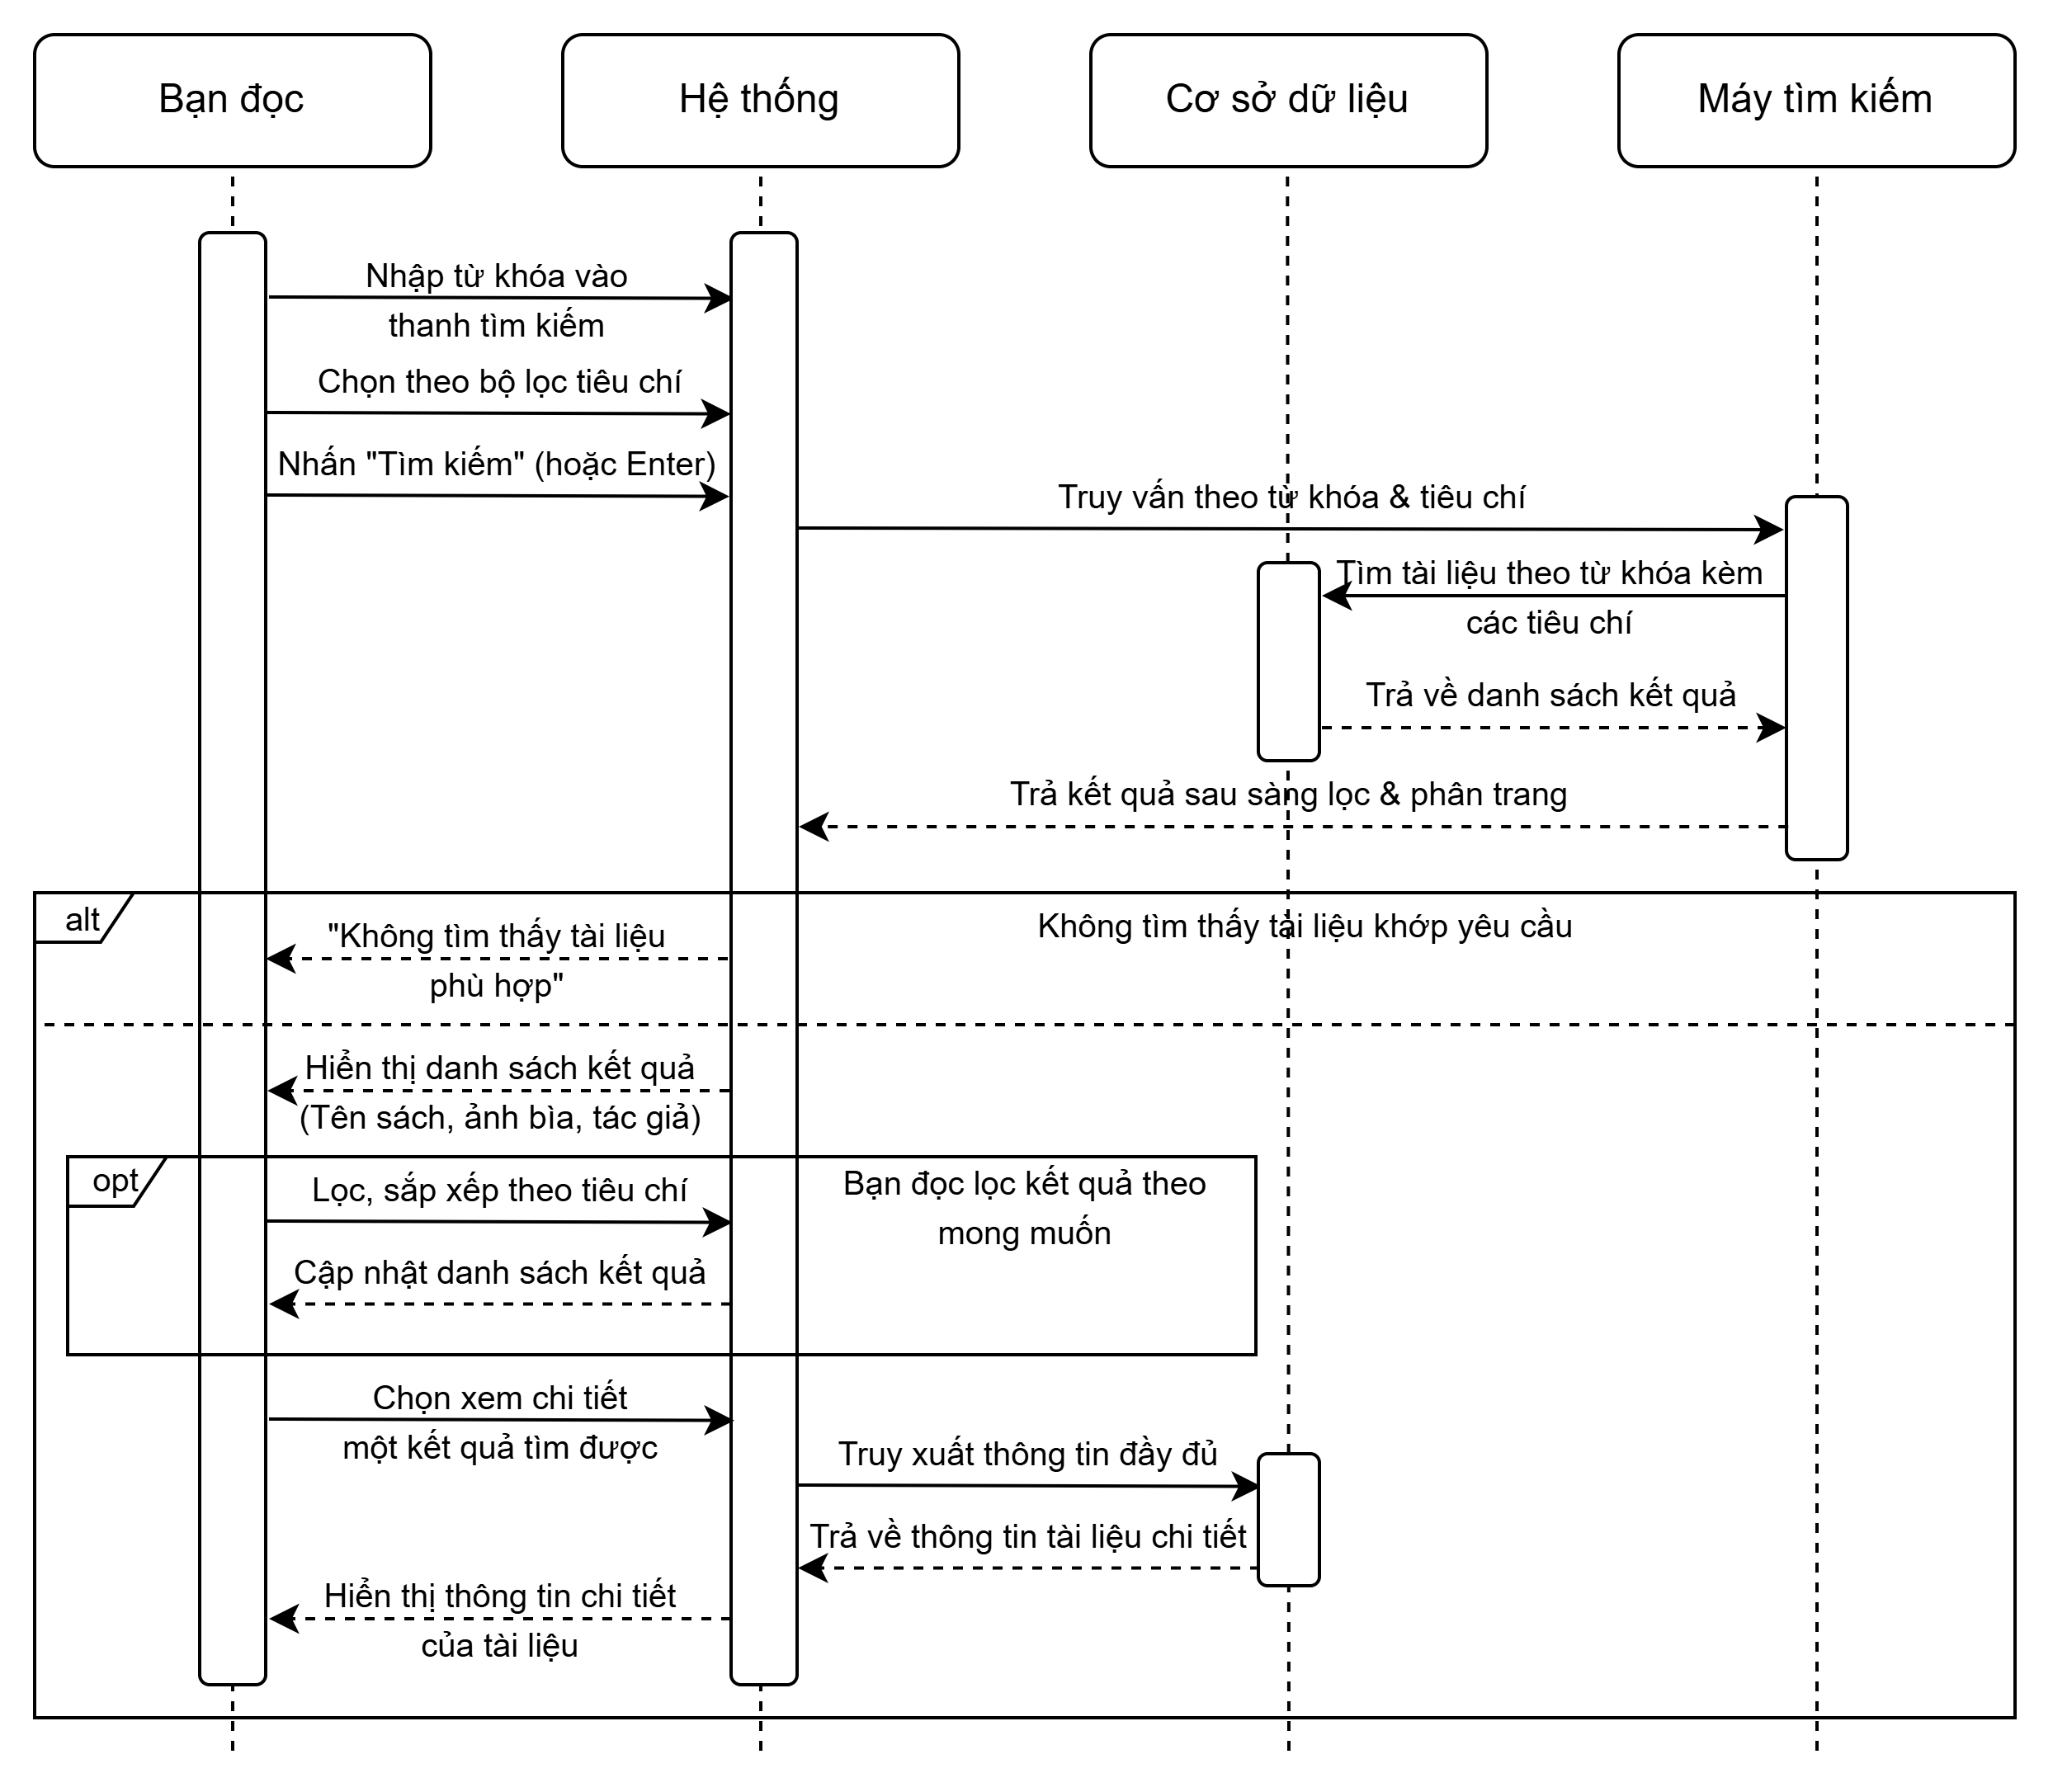
\includegraphics[width=0.6\linewidth]{Images/Seq_Tim kiem.png}
    \vspace{10pt}
    \caption{Sơ đồ tuần tự Tìm kiếm tài liệu}
    \label{fig:sequence_search}
\end{figure}
\begin{enumerate}
    \item Bạn đọc tiến hành nhập từ khóa vào thanh tìm kiếm, sau đó có thể bổ sung tiêu chí tìm kiếm tương ứng.
    \item Sau khi bạn đọc nhấn "Tìm kiếm" hoặc phím Enter, hệ thống gửi dữ liệu đến máy tìm kiếm (search engine), máy tìm kiếm tiến hành phối hợp với cơ sở dữ liệu để tìm tài liệu phù hợp với yêu cầu của bạn đọc, sau đó trả về kết quả đã qua sàng lọc và phân trang.
    \item Nếu danh sách kết quả rỗng, hệ thống báo "Không tìm thấy tài liệu phù hợp", \textbf{kết thúc quy trình tại đây}. Nếu không, tiến hành hiển thị danh sách kết quả sau khi tiến hành truy vấn, mỗi kết quả đều hiển thị thông tin cơ bản của tài liệu (bao gồm bìa sách, tên tài liệu, tác giả, ...).
    \item Khi bạn đọc có nhu cầu lọc kết quả, hệ thống sàng lọc kết quả từ danh sách nhận về từ máy tìm kiếm.
    \item Bạn đọc khi chọn xem chi tiết một kết quả tìm được, hệ thống gửi truy vấn cụ thể về cơ sở dữ liệu nhằm lấy thông tin đầy đủ về tài liệu tương ứng, sau đó hiển thị thông tin đầy đủ cho bạn đọc.
\end{enumerate}
\subsubsection{Thêm/sửa/xóa tài liệu}
\subsubsubsection{Thêm tài liệu}
\begin{figure}[H]
    \centering
    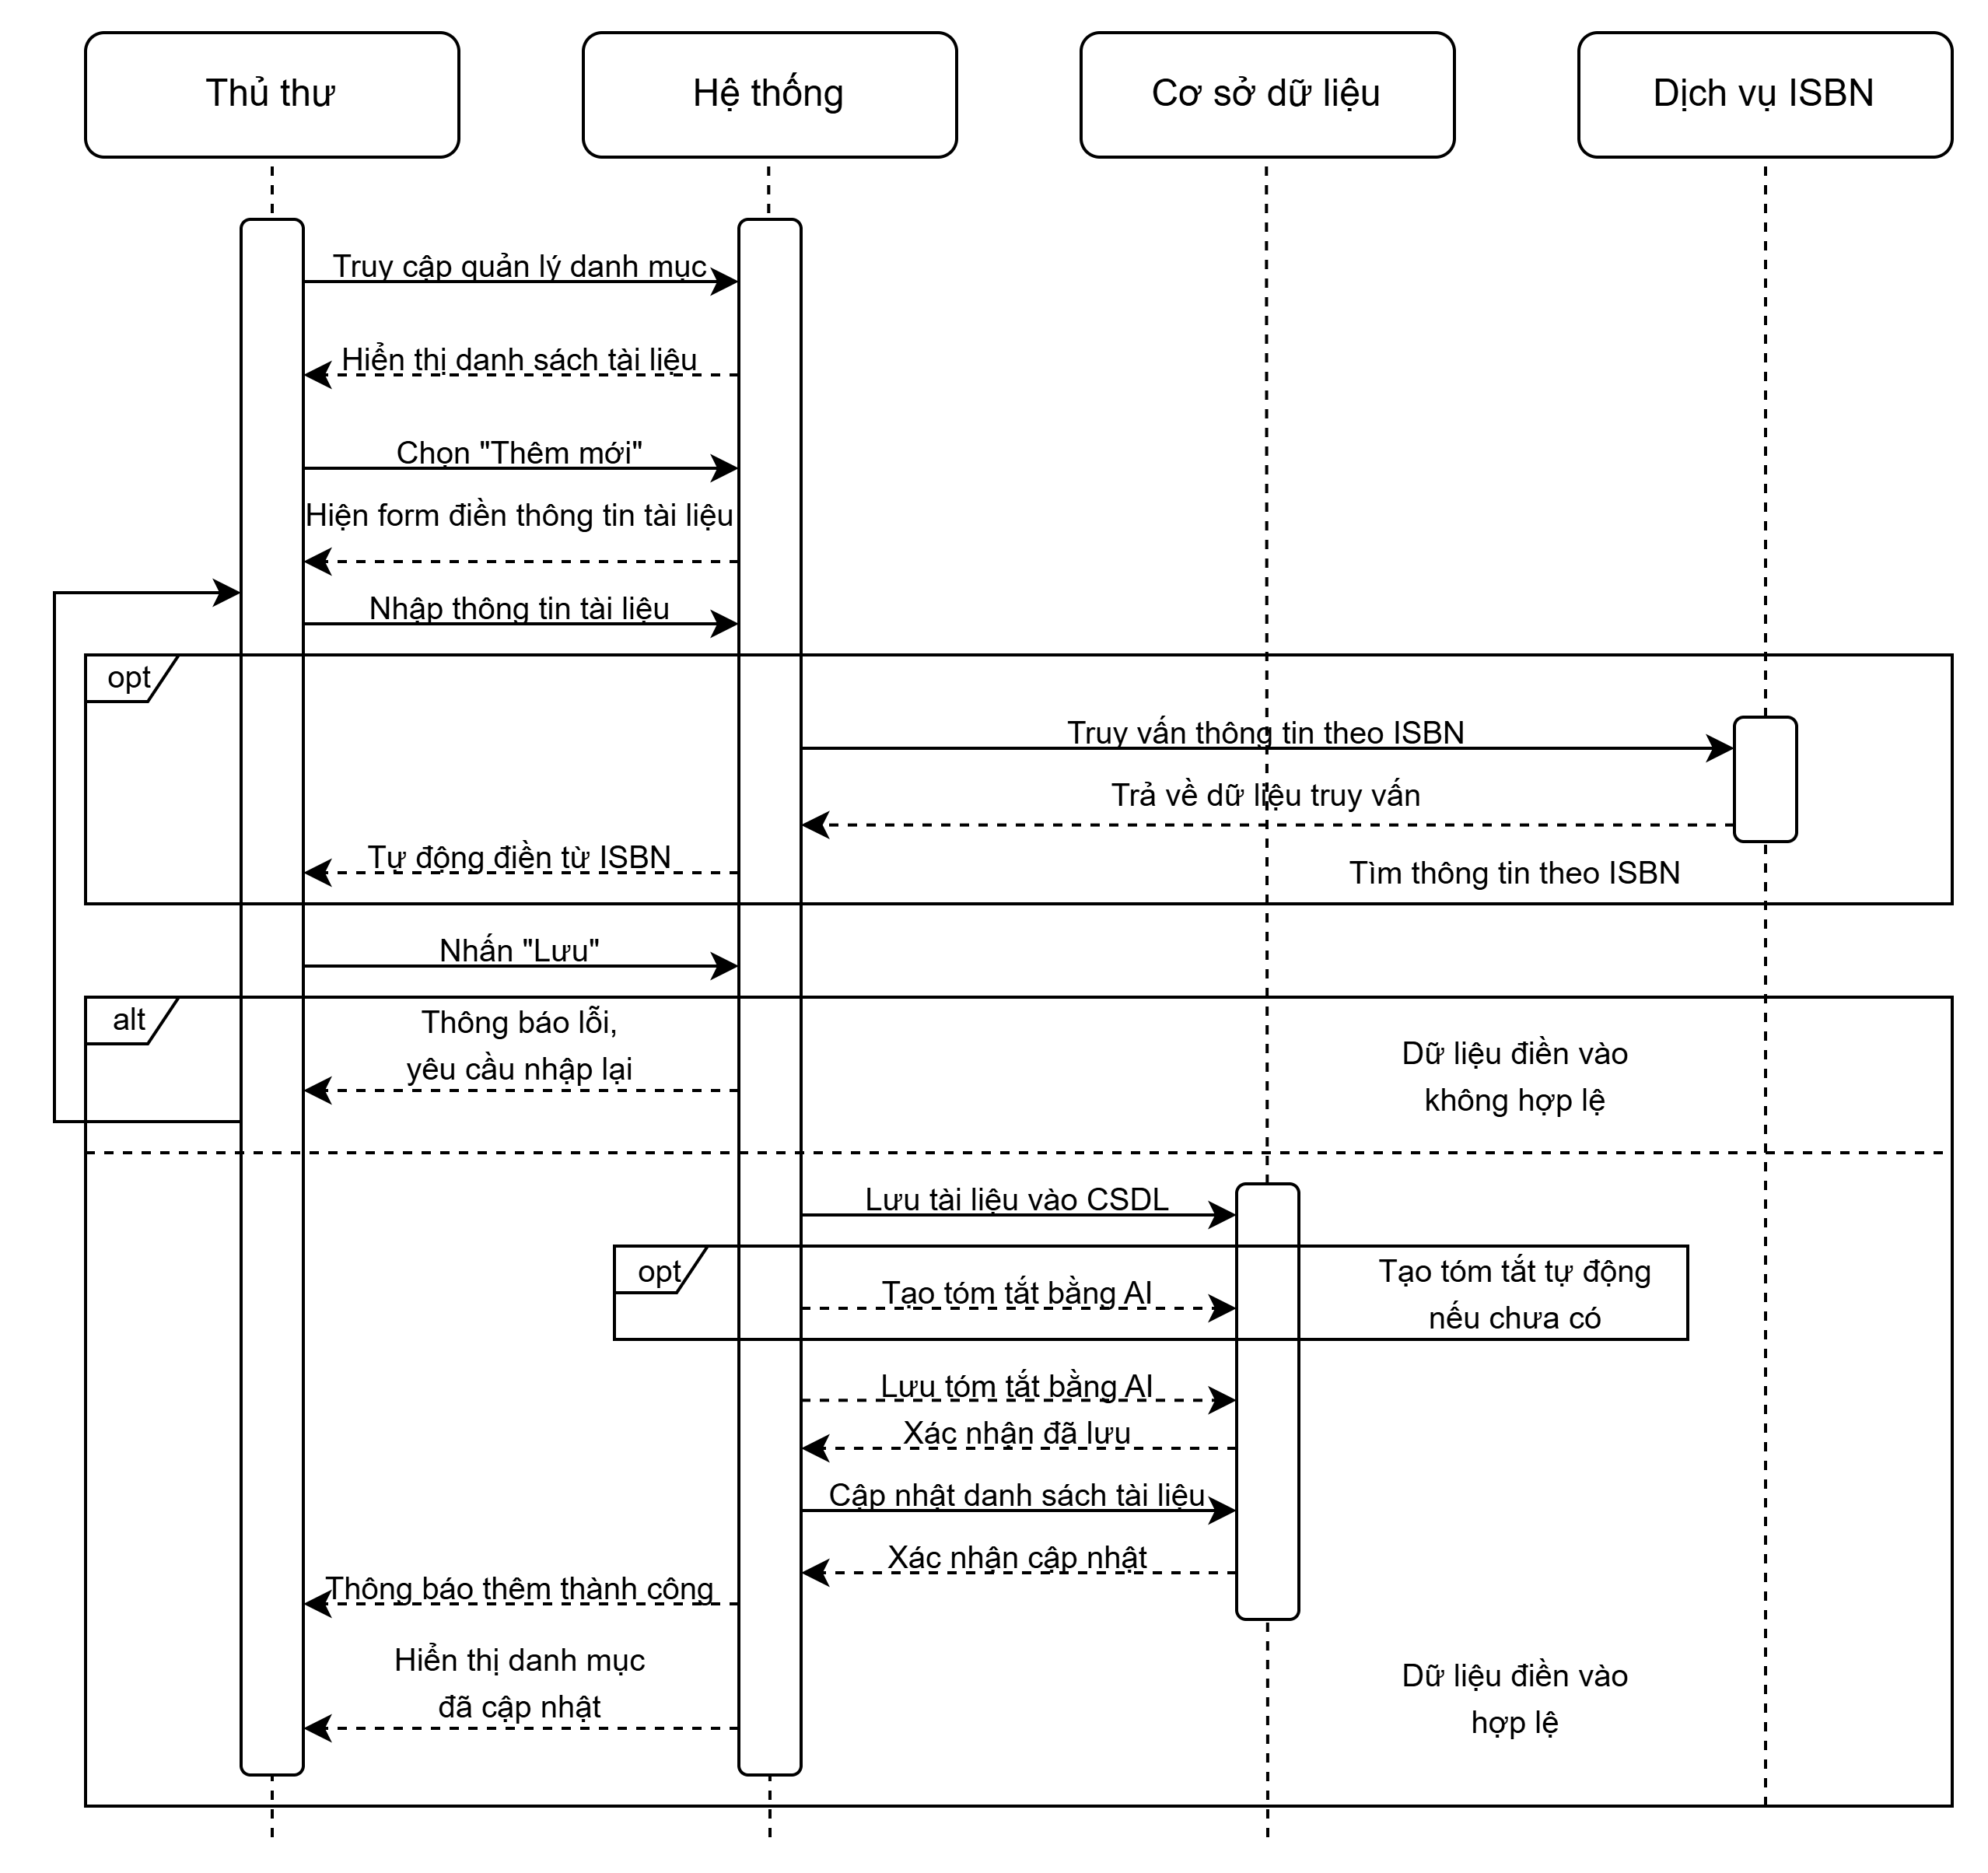
\includegraphics[width=0.6\linewidth]{Images/Seq_Them tai lieu.png}
    \vspace{10pt}
    \caption{Sơ đồ tuần tự Thêm tài liệu}
    \label{fig:sequence_add_document}
\end{figure}
\begin{enumerate}
    \item Thủ thư tiến hành truy cập "Quản lý danh mục" và chọn "Thêm mới" để thêm tài liệu.
    \item Khi tiến hành "Thêm mới", biểu mẫu thông tin tài liệu và tùy chọn "Nhập theo mã ISBN".
    \begin{itemize}
        \item Nếu thủ thư sử dụng "Nhập theo mã ISBN", hệ thống truy xuất thông tin từ dịch vụ ISBN và tự động điền vào biểu mẫu.
        \item Nếu không, thủ thư nhập thông tin thủ công về tài liệu cần được thêm vào.
    \end{itemize}
    \item Khi thủ thư nhấn "Lưu", hệ thống tiến hành kiểm tra thông tin hợp lệ hay không:
    \begin{itemize}
        \item Nếu thông tin hợp lệ, hệ thống lưu tài liệu vào cơ sở dữ liệu, sau đó cập nhật danh sách tài liệu hiện có. Nếu không, hệ thống báo lỗi, yêu cầu thủ thư sửa lại thông tin không hợp lệ trước khi lưu tài liệu.
        \item Thủ thư có thể sử dụng tính năng "Tóm tắt bằng AI" nhằm tóm tắt nội dung bằng AI trước khi lưu cùng thông tin tài liệu thêm mới.
    \end{itemize}
    \item Sau khi hoàn thành lưu tài liệu, quá trình thêm mới hoàn thành.
\end{enumerate}
\subsubsubsection{Sửa tài liệu}
\begin{figure}[H]
    \centering
    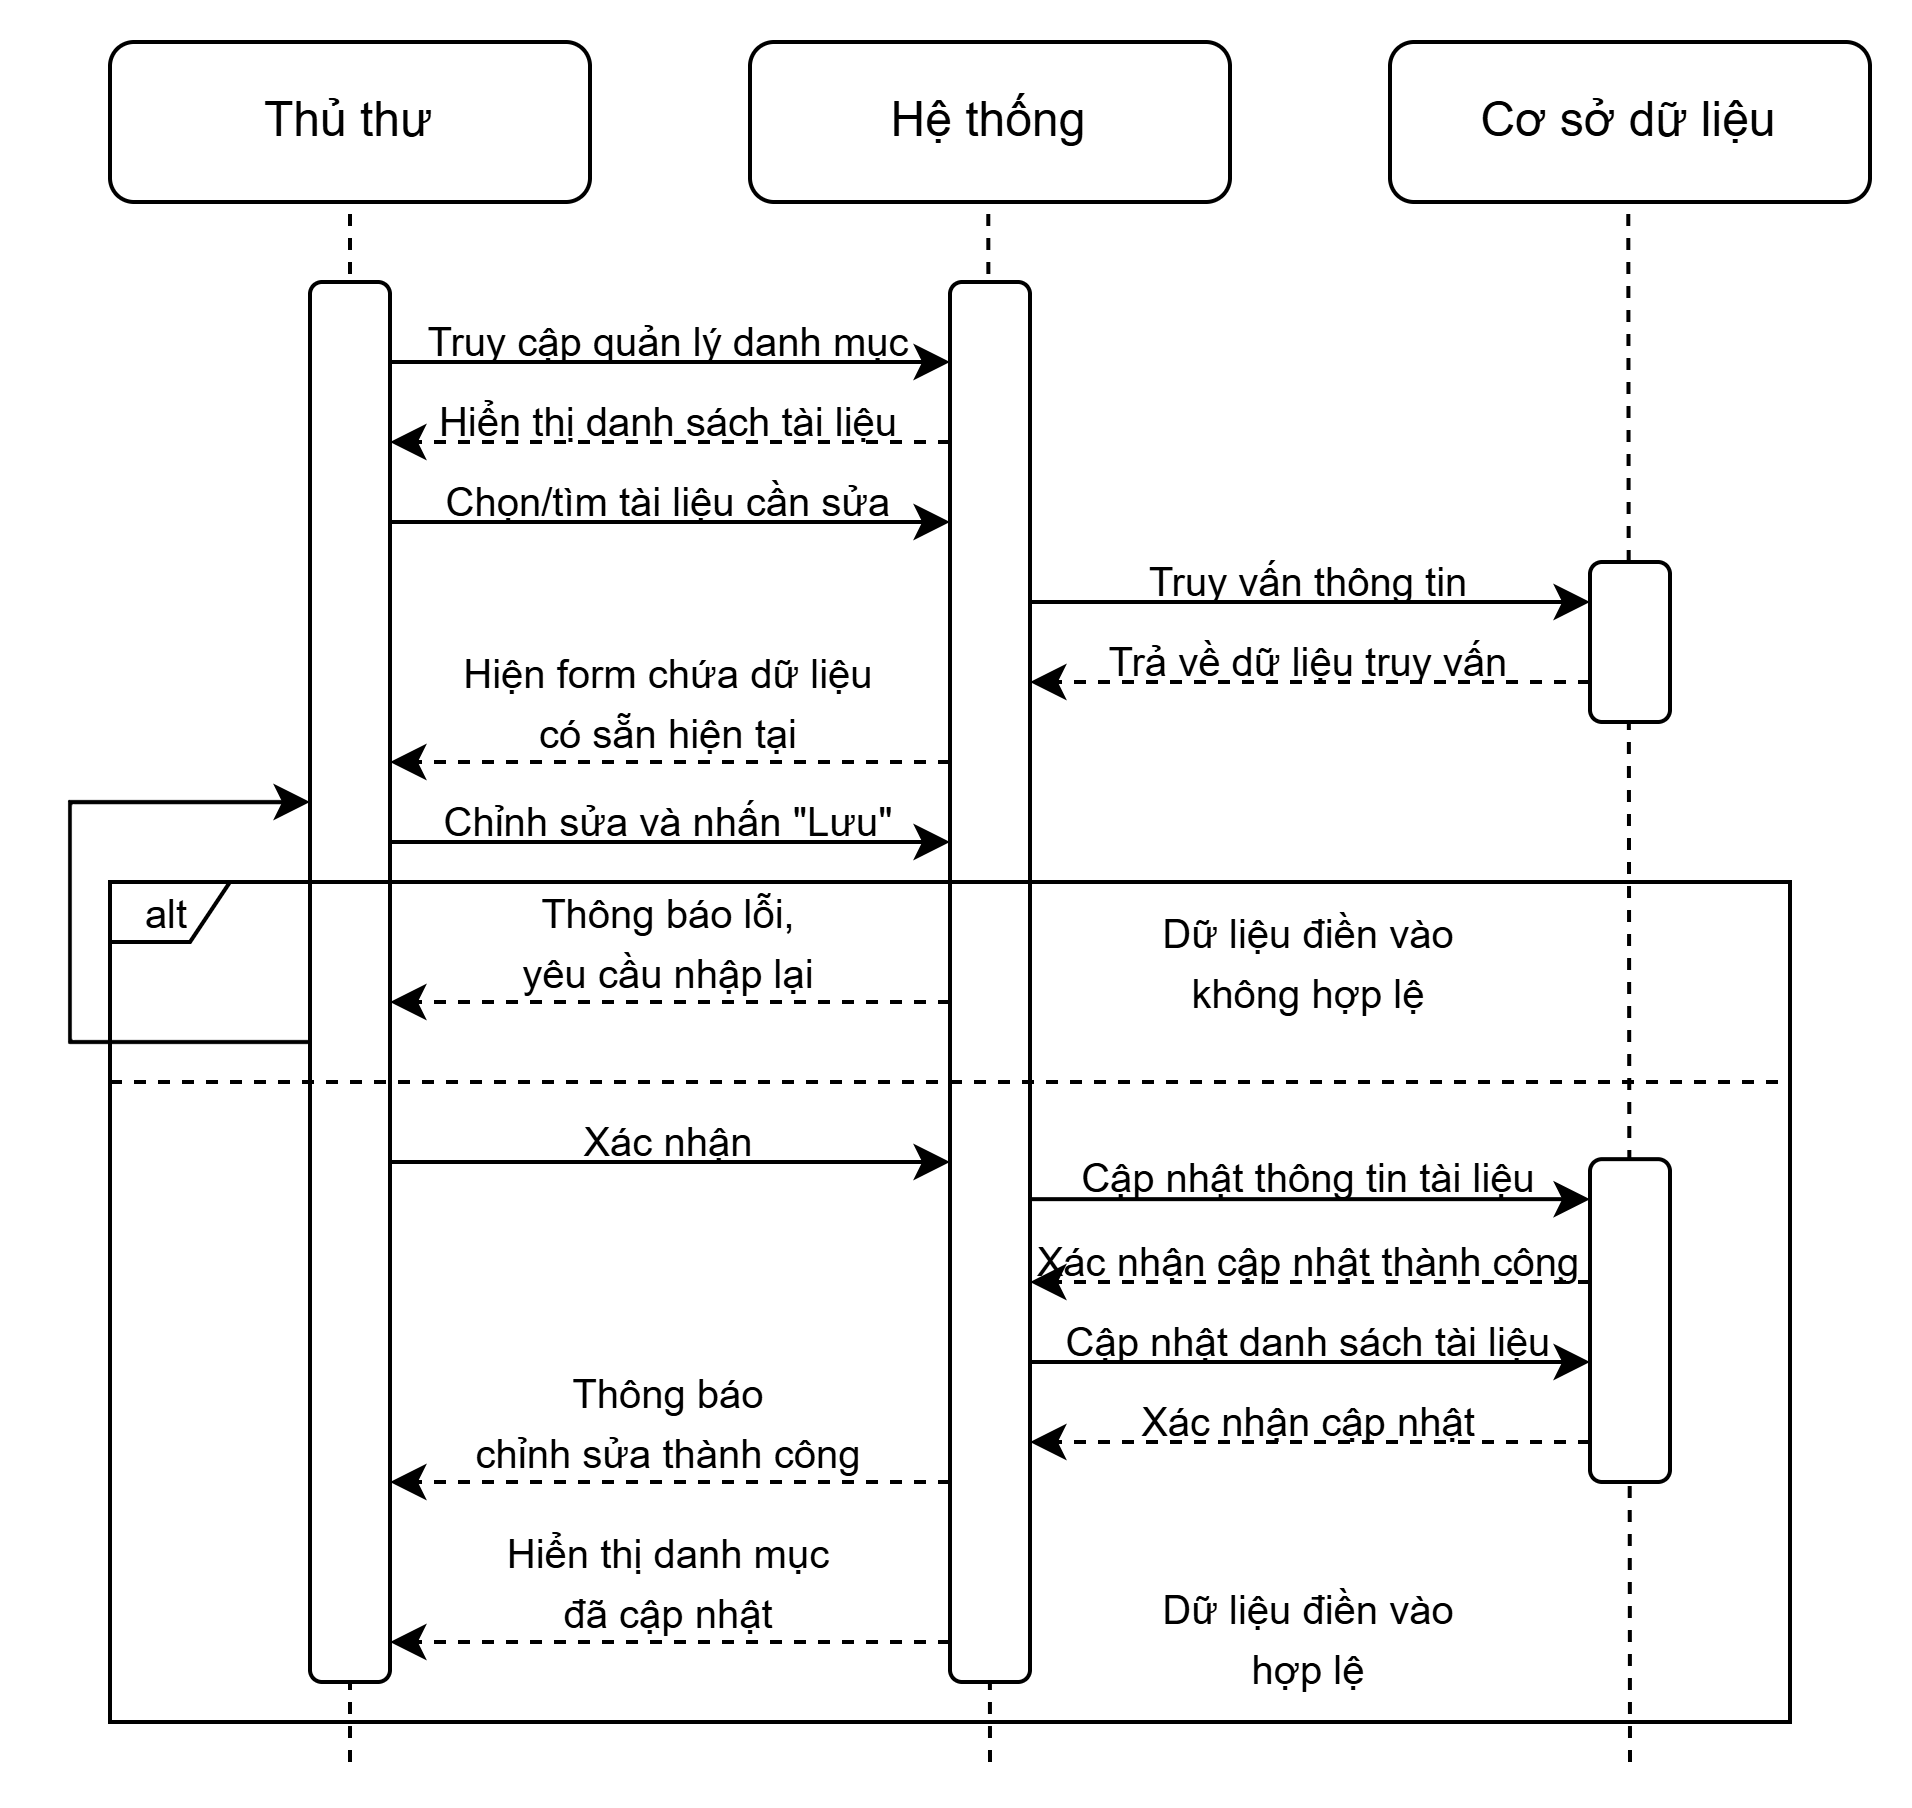
\includegraphics[width=0.6\linewidth]{Images/Seq_Sua tai lieu.png}
    \vspace{10pt}
    \caption{Sơ đồ tuần tự Sửa tài liệu}
    \label{fig:sequence_edit_document}
\end{figure}
\begin{enumerate}
    \item Thủ thư tiến hành truy cập "Quản lý danh mục" và chọn tài liệu cần sửa. Sau đó, hệ thống tự động truy vấn thông tin tài liệu cần sửa và trả về cho thủ thư dưới dạng biểu mẫu đã điền sẵn.
    \item Thủ thư tiến hành chỉnh sửa thông tin tài liệu, sau đó nhấn "Lưu". Hệ thống kiểm tra tính hợp lệ của các thông tin đã được sửa.
    \begin{itemize}
        \item Nếu thông tin hợp lệ, hệ thống cập nhật thông tin tài liệu trên cơ sở dữ liệu và cập nhật danh sách, thông báo "Cập nhật thành công" cho thủ thư.
        \item Nếu thông tin \textbf{không hợp lệ}, hệ thống báo lỗi, thủ thư cần chỉnh sửa lại thông tin không hợp lệ trước khi cập nhật lại.
    \end{itemize}
    \item Sau khi cập nhật thành công, quy trình kết thúc.
\end{enumerate}
\subsubsubsection{Xóa tài liệu}
\begin{figure}[H]
    \centering
    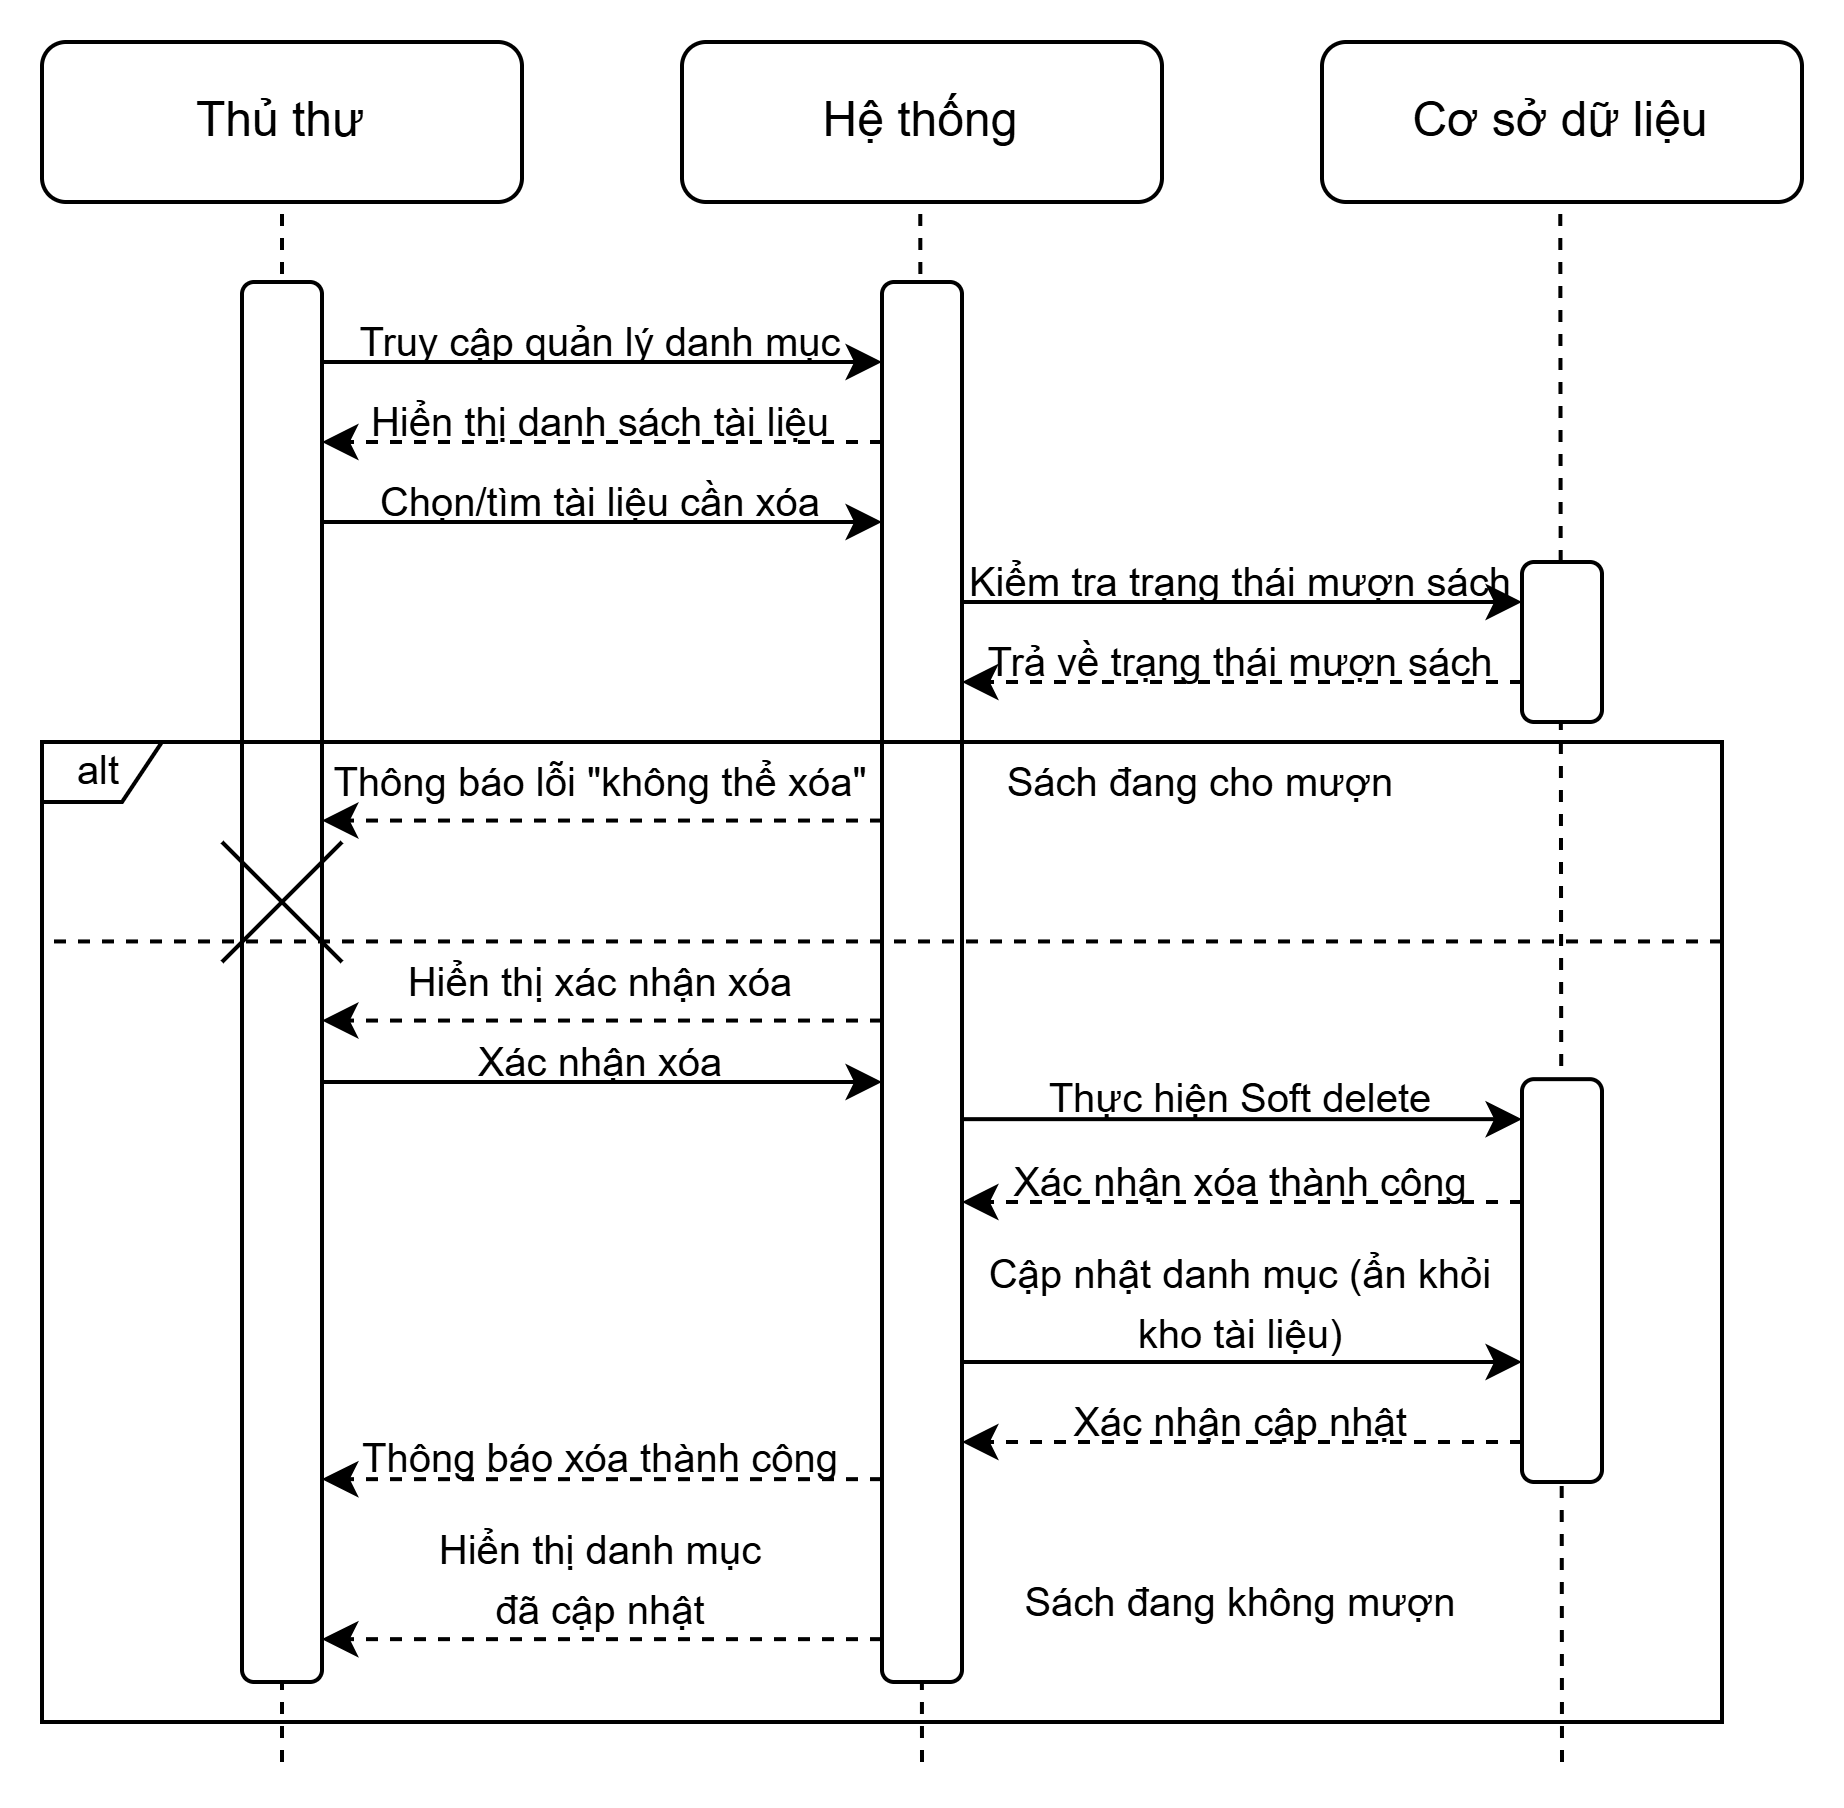
\includegraphics[width=0.6\linewidth]{Images/Seq_Xoa tai lieu.png}
    \vspace{10pt}
    \caption{Sơ đồ tuần tự Xóa tài liệu}
    \label{fig:sequence_delete_document}
\end{figure}
\begin{enumerate}
    \item Thủ thư tiến hành truy cập "Quản lý danh mục" và chọn tài liệu cần xóa. Hệ thống tự động kiểm tra trạng thái sách nhằm tránh xóa nhầm tài liệu đang cho mượn.
    \item Nếu sách đang cho mượn, hệ thống báo lỗi "Không thể xóa", quy trình \textbf{kết thúc tại đây}. Nếu không, hệ thống cần thủ thư xác nhận xóa trước khi tiến hành Soft delete (xóa khỏi danh sách tài liệu nhưng không xóa khỏi cơ sở dữ liệu).
    \item Sau khi thực hiện Soft delete, hệ thống thông báo "Xóa thành công" và cập nhật danh sách. Quy trình kết thúc.
\end{enumerate}
\subsubsection{Thêm tài liệu hàng loạt}
\begin{figure}[H]
    \centering
    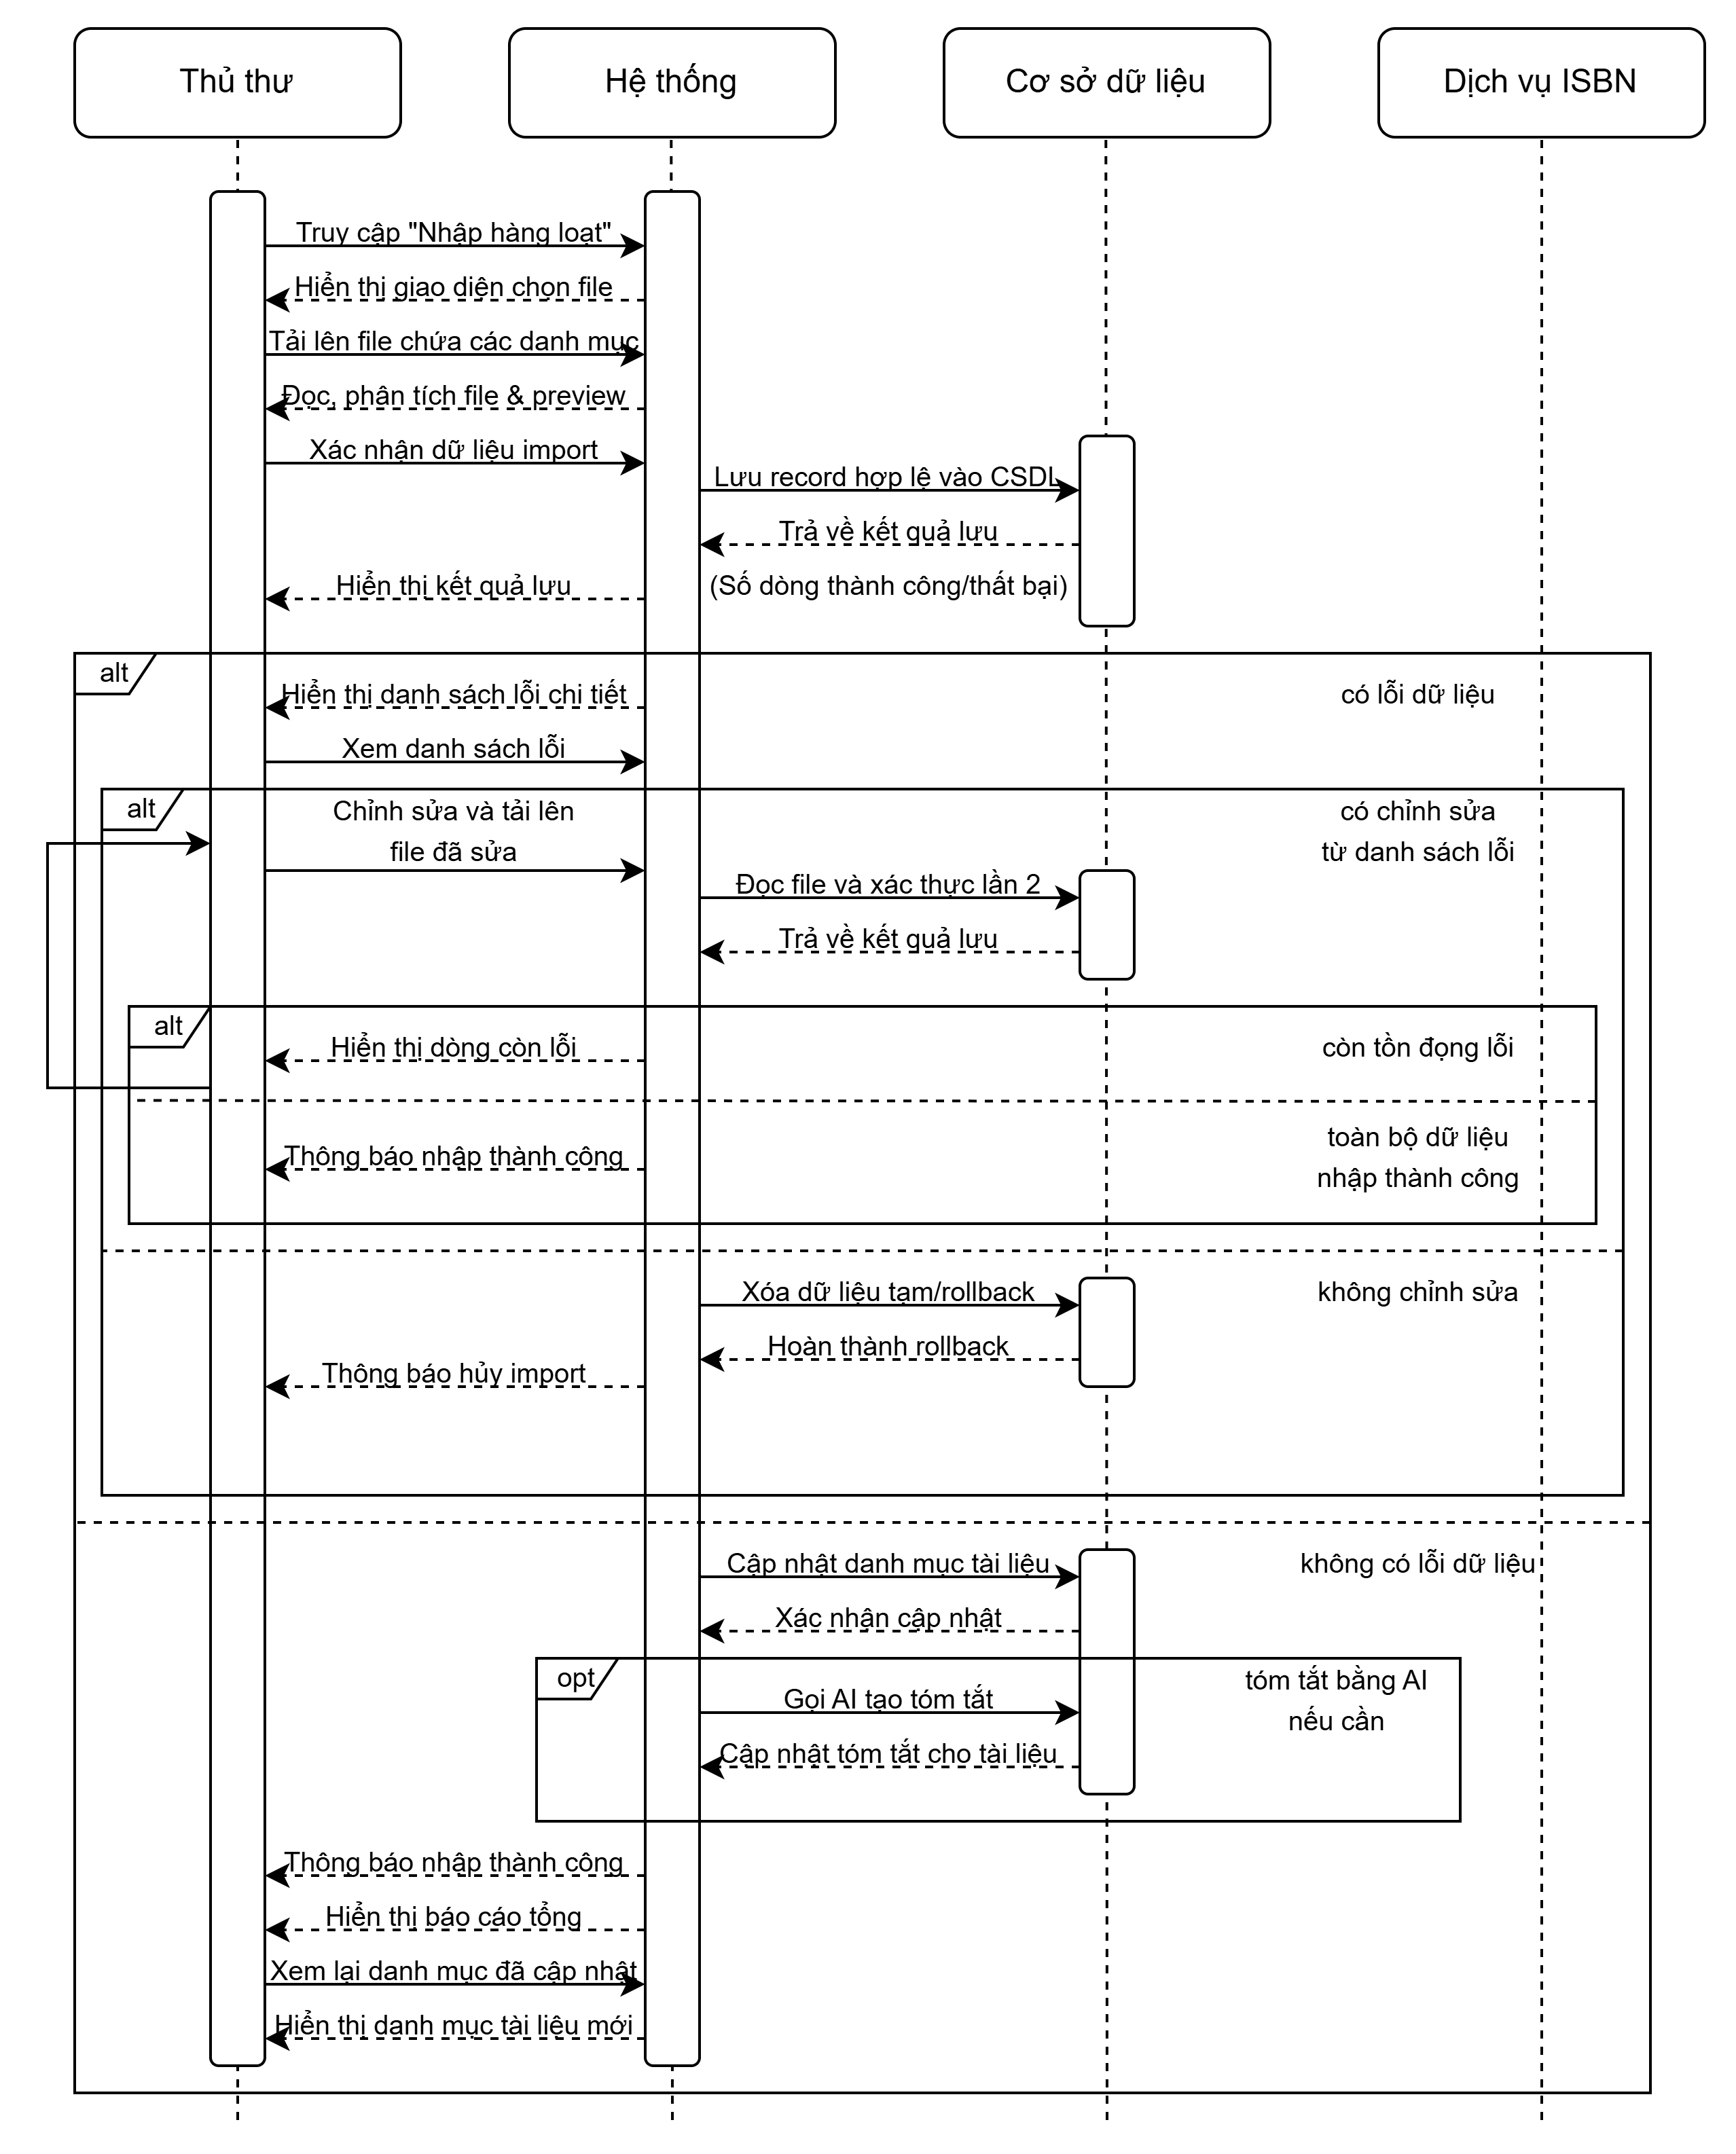
\includegraphics[width=0.6\linewidth]{Images/Seq_Them hang loat.png}
    \vspace{10pt}
    \caption{Sơ đồ tuần tự Thêm tài liệu hàng loạt}
    \label{fig:sequence_import_documents}
\end{figure}
\begin{enumerate}
    \item Từ trang "Quản lý danh mục", thủ thư chọn "Nhập hàng loạt", sau đó nhập dữ liệu hàng loạt bằng file.
    \item Sau khi thủ thư xác nhận dữ liệu, hệ thống tiến hành kiểm tra thông tin của từng tài liệu trong file, sau đó ghi nhận số dòng thành công/lỗi và thông báo cho thủ thư.
    \begin{itemize}
        \item Nếu toàn bộ tài liệu trong file thành công, hệ thống thông báo cho thủ thư, sau đó tiến hành cập nhật tổng và hiển thị.
        \item Nếu có dòng chứa thông tin không hợp lệ, thông báo lỗi cho thủ thư, sau đó thủ thư tiến hành sửa lại dòng chứa thông tin không hợp lệ trước khi tải lên file.
    \end{itemize}
    Nếu thủ thư không chỉnh sửa file, hệ thống tiến hành rollback và thông báo hủy nhập hàng loạt.
\end{enumerate}
\subsubsection{Đặt mượn tài liệu}
\begin{figure}[H]
    \centering
    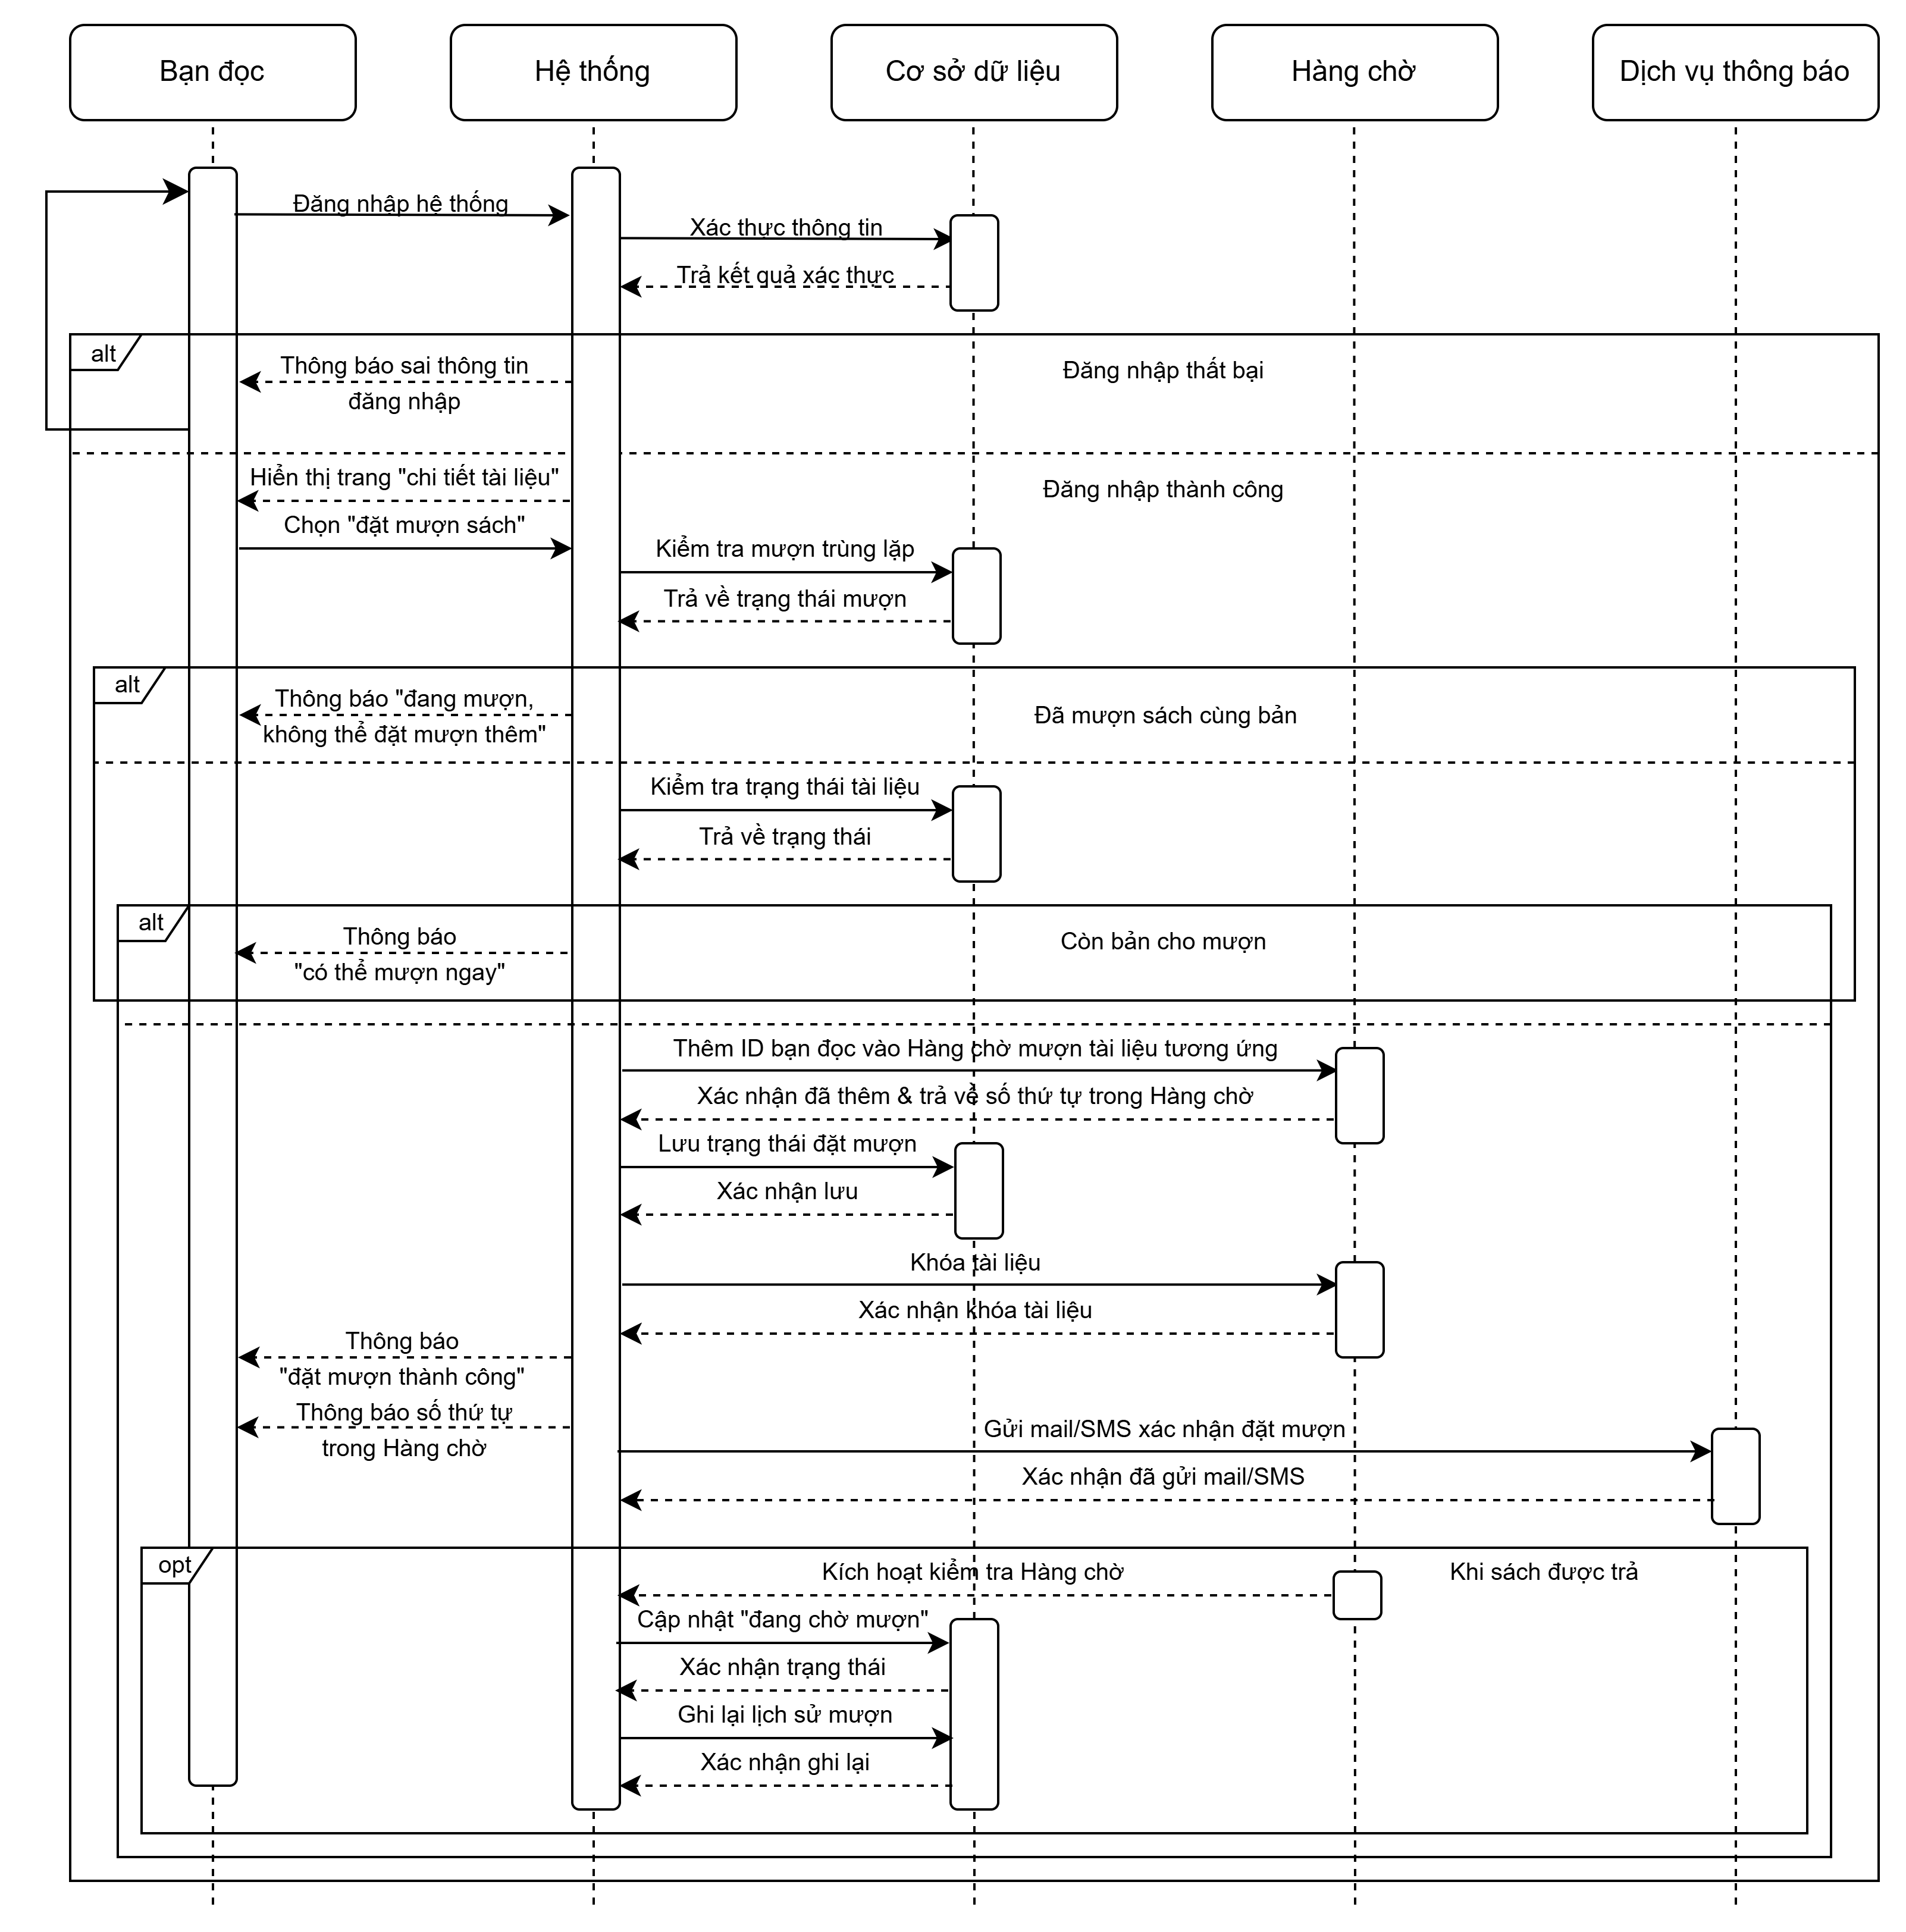
\includegraphics[width=0.6\linewidth]{Images/Seq_Dat muon sach.png}
    \vspace{10pt}
    \caption{Sơ đồ tuần tự Đặt mượn tài liệu}
    \label{fig:sequence_reserve_document}
\end{figure}
\begin{enumerate}
    \item Khi mượn tài liệu, bạn đọc cần đăng nhập tài khoản. Nếu đã đăng nhập tài khoản, bước này có thể bỏ qua.
    \item Trong quá trình xem thông tin chi tiết về tài liệu, khi tiến hành chọn "Đặt mượn tài liệu", hệ thống kiểm tra mượn trùng lặp tài liệu. Nếu phát hiện mượn trùng lặp tài liệu, hệ thống từ chối với lý do "Đã mượn tài liệu đang chọn, không thể mượn thêm".
    \item Sau khi kiểm tra mượn trùng lặp, hệ thống kiểm tra số bản còn trong kho thư viện.
    \begin{enumerate}
        \item Nếu còn bản trong kho, hệ thống báo về "Có thể mượn ngay", bạn đọc có thể gửi yêu cầu mượn đến thủ thư để mượn tài liệu.
        \item Khi không còn bản có sẵn, bạn đọc được đưa vào hàng chờ mượn tài liệu và hiển thị số thứ tự trong hàng chờ hiện tại, sau đó tài liệu được khóa để tránh bị xóa. Đồng thời, hệ thống gửi email xác nhận mượn tài liệu của bạn đọc.
    \end{enumerate}
    \item Sau này, khi tài liệu được trả về, hệ thống tiến hành cập nhật hàng đợi và thông báo đến bạn đọc tiếp theo.
\end{enumerate}
\subsubsection{Cập nhật tiền phạt}
\begin{figure}[H]
    \centering
    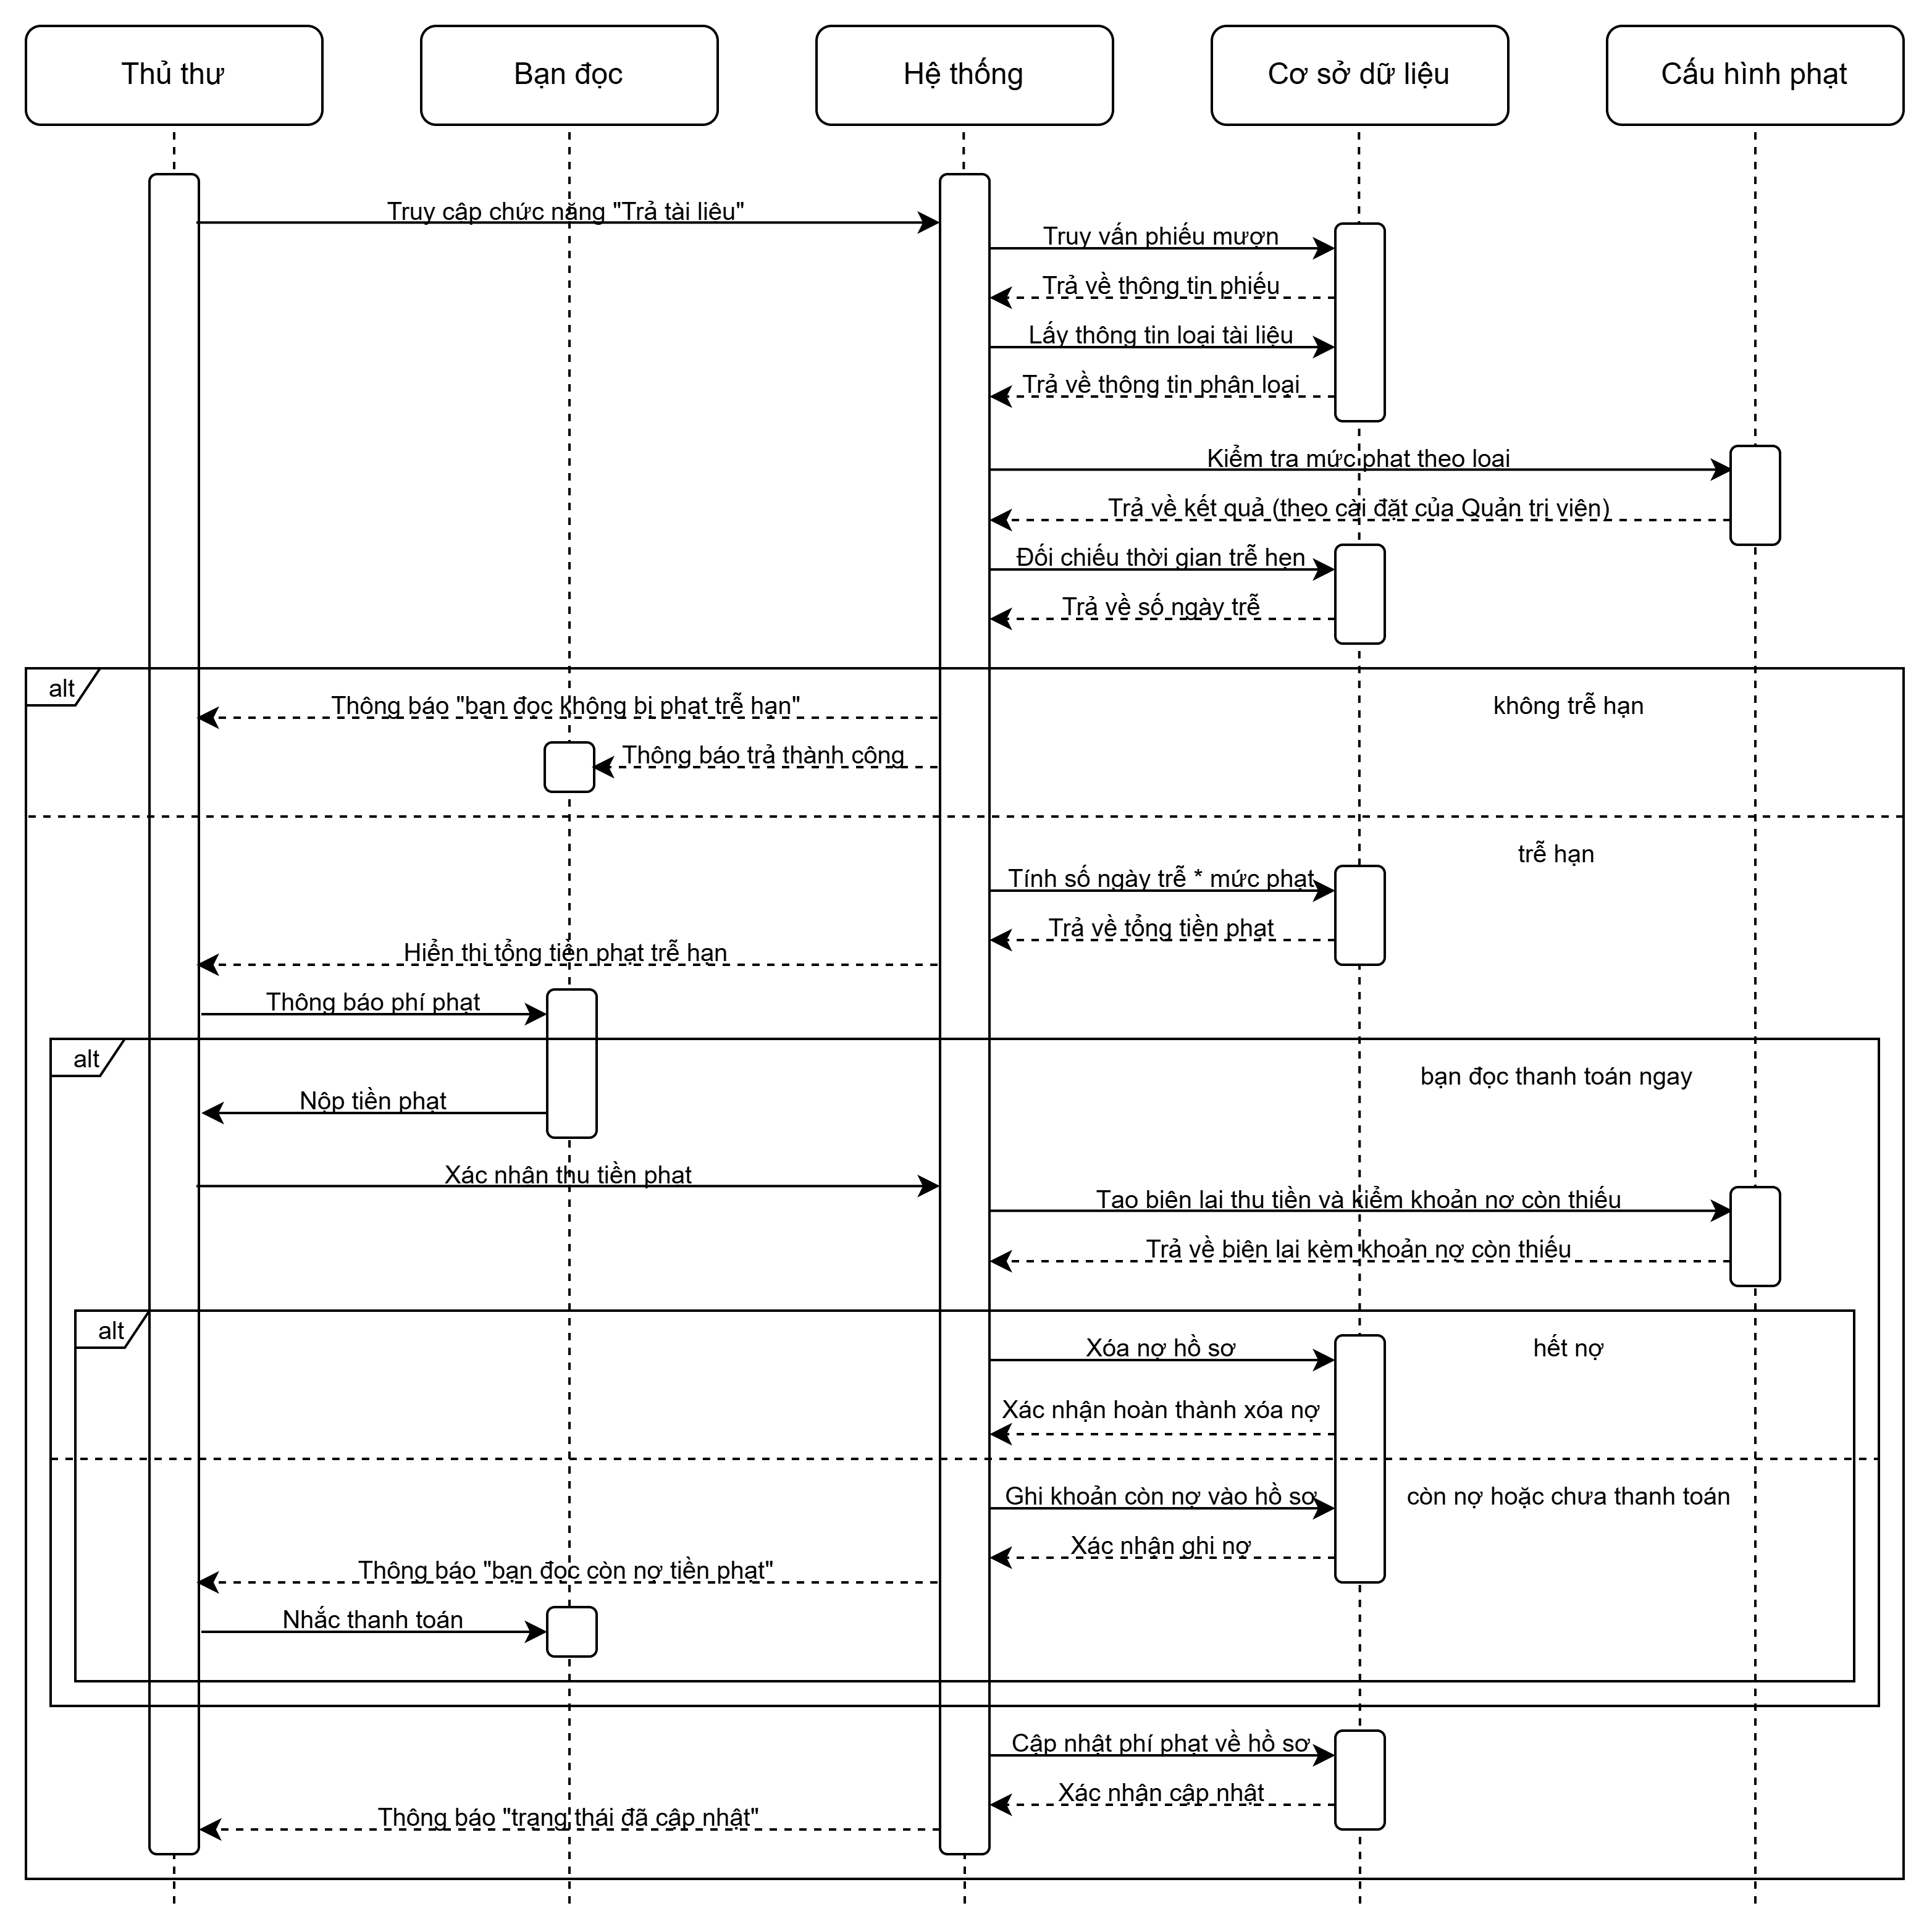
\includegraphics[width=0.6\linewidth]{Images/Seq_Tien phat.png}
    \vspace{10pt}
    \caption{Sơ đồ tuần tự Cập nhật tiền phạt}
    \label{fig:sequence_fine}
\end{figure}
\begin{enumerate}
    \item Thủ thư tiến hành đăng nhập hệ thống và lấy mã định danh bạn đọc từ cơ sở dữ liệu để xử lý yêu cầu mượn tài liệu.
    \item Với các yêu cầu bạn đọc, hệ thống tự động kiểm tra mức nợ tiền phạt và số lượng tài liệu đang mượn, đối chiếu với định mức tiền phạt và giới hạn mượn tài liệu.
    \item Nếu tài khoản bạn đọc không hợp lệ hoặc tổng nợ phí phạt vượt định mức, hoặc số lượng tài liệu đang mượn của bạn đọc đạt tối đa, hệ thống tự động từ chối yêu cầu, \textbf{quá trình xử lý mượn tài liệu kết thúc}. Nếu không, hệ thống bắt đầu quá trình mượn tài liệu cho bạn đọc.
    \item Thủ thư thực hiện quét các tài liệu mà bạn đọc muốn mượn.
    \item Sau khi hoàn thành quét các tài liệu, hệ thống tạo phiếu mượn song song với việc tính toán thời hạn mượn theo từng loại tài liệu. Sau đó, hệ thống ghi lại lịch sử mượn tài liệu và trừ số bản có sẵn trong kho trước khi hiển thị phiếu mượn kèm hạn trả.
    \item Thủ thư giao tài liệu cho bạn đọc, quá trình xử lý mượn tài liệu kết thúc.
\end{enumerate}
\subsubsection{Xử lý mượn Tài liệu}
\begin{figure}[H]
    \centering
    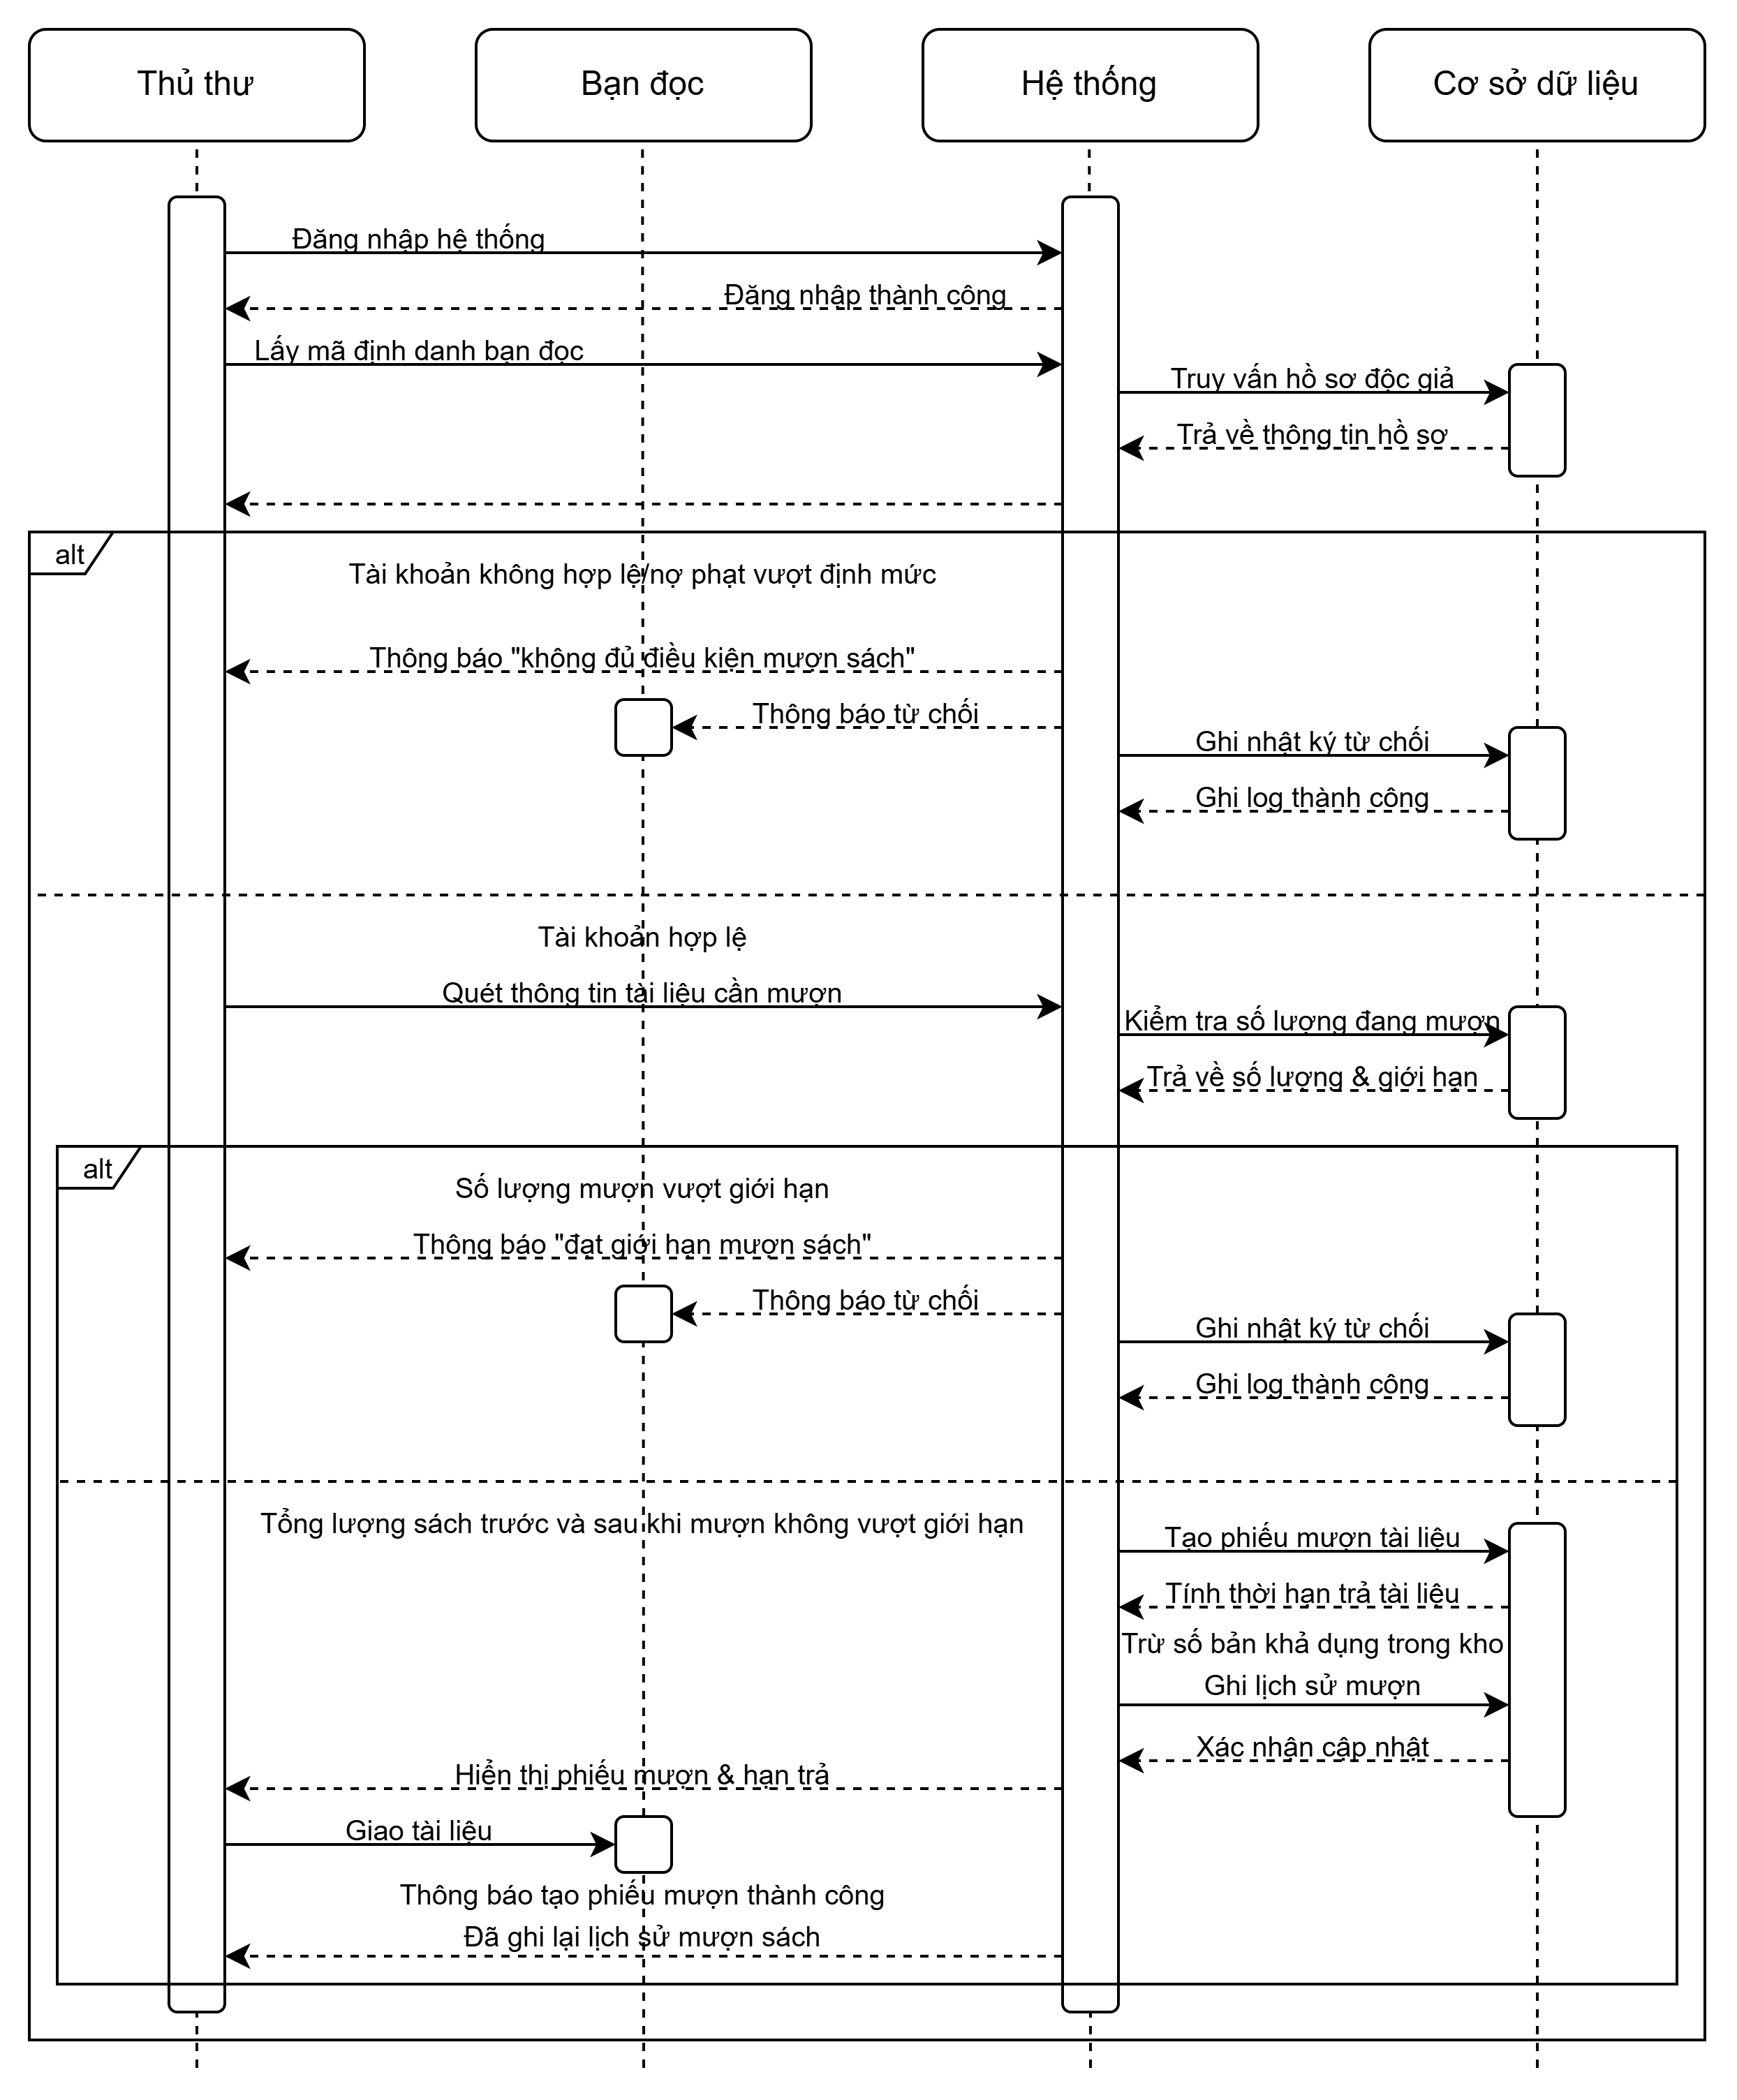
\includegraphics[width=0.6\linewidth]{Images/Seq_Muon sach.png}
    \vspace{10pt}
    \caption{Sơ đồ tuần tự Xử lý mượn Tài liệu}
    \label{fig:sequence_borrow}
\end{figure}
\begin{enumerate}
    \item Khi thủ thư tiếp nhận yêu cầu mượn tài liệu từ bạn đọc, hệ thống tự động kiểm tra tính hợp lệ của tài khoản bạn đọc và điều kiện mượn tài liệu.
    \begin{itemize}
        \item Nếu tài khoản bạn đọc không hợp lệ hoặc tổng nợ phí phạt vượt định mức, hoặc số lượng tài liệu đang mượn của bạn đọc đạt tối đa, hệ thống tự động từ chối yêu cầu, \textbf{quá trình xử lý mượn tài liệu kết thúc}. Nếu không, hệ thống bắt đầu quá trình mượn tài liệu cho bạn đọc.
        \item Nếu có tài liệu nào trong yêu cầu mượn đang được đặt giữ chỗ (Reserve) bởi người khác, hệ thống từ chối yêu cầu mượn với lý do "Tài liệu đang được đặt giữ chỗ bởi người khác", \textbf{quy trình kết thúc}. Nếu không, quy trình tiếp tục.
        \item Nếu tổng số tài liệu sau khi mượn vượt quá giới hạn mượn, hệ thống từ chối yêu cầu mượn với lý do "Vượt quá giới hạn mượn", \textbf{quy trình kết thúc}. Nếu không, quy trình khởi tạo phiếu mượn cho bạn đọc, đồng thời trừ số bản có sẵn trong kho trước khi hiển thị thông tin cụ thể cho thủ thư.
    \end{itemize}
    \item Sau khi thủ thư gửi thông tin phiếu mượn và giao tài liệu cho bạn đọc, hệ thống cập nhật lịch sử mượn tài liệu.
\end{enumerate}
\subsubsection{Gia hạn mượn tài liệu}
\begin{figure}[H]
    \centering
    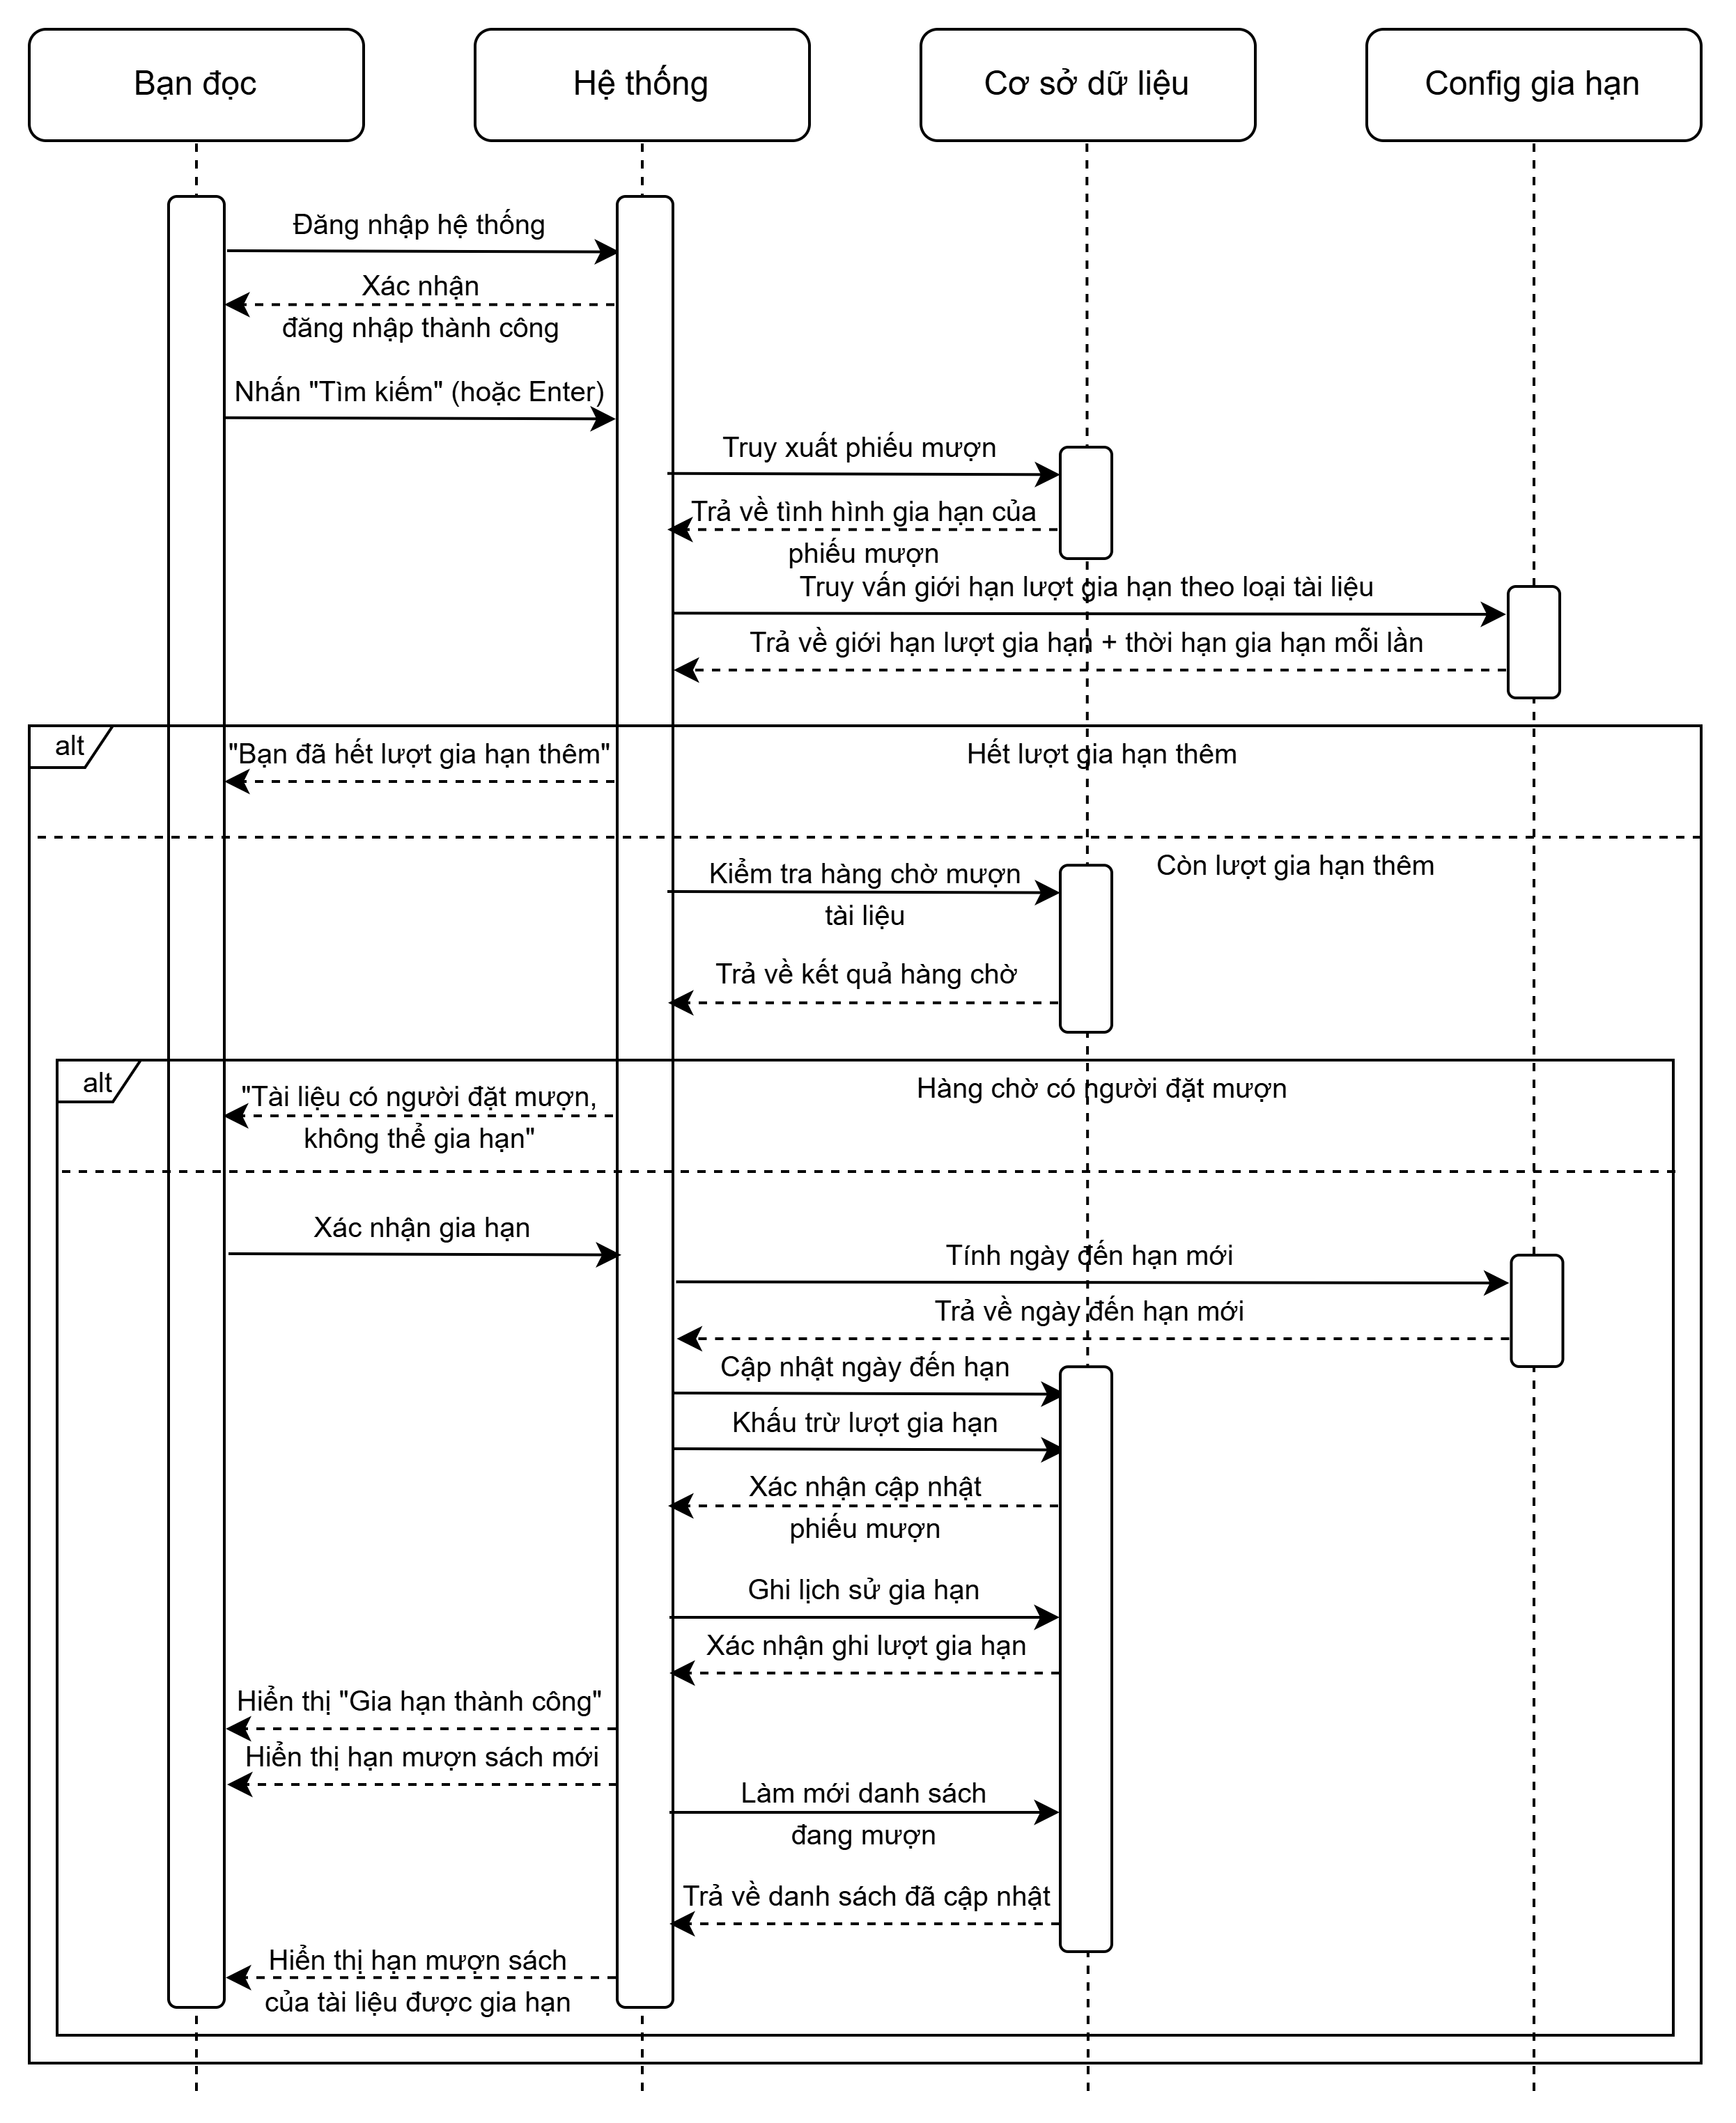
\includegraphics[width=0.6\linewidth]{Images/Seq_Gia han.png}
    \vspace{10pt}
    \caption{Sơ đồ tuần tự Gia hạn mượn tài liệu}
    \label{fig:sequence_extend_borrow}
\end{figure}
\begin{enumerate}
    \item Bạn đọc tiến hành đăng nhập và kiểm tra tình trạng phiếu mượn, hệ thống trả về thời hạn trả tài liệu kèm số lần gia hạn còn lại.
    \item Khi bạn đọc yêu cầu gia hạn:
    \begin{itemize}
        \item Nếu không còn lượt gia hạn hoặc có tài liệu được đặt mượn trong danh sách tài liệu đang mượn, hệ thống từ chối với lý do tương ứng. Quá trình gia hạn mượn tài liệu \textbf{kết thúc}.
        \item Nếu không, hệ thống tự động trừ một lượt gia hạn của phiếu mượn, tiến hành cập nhật hạn trả tài liệu mới và cập nhật vào phiếu mượn có chứa tài liệu muốn gia hạn, thông báo "Gia hạn thành công" và hiển thị hạn mượn tài liệu mới.
    \end{itemize}
\end{enumerate}
\subsubsection{Trả tài liệu}
\begin{figure}[H]
    \centering
    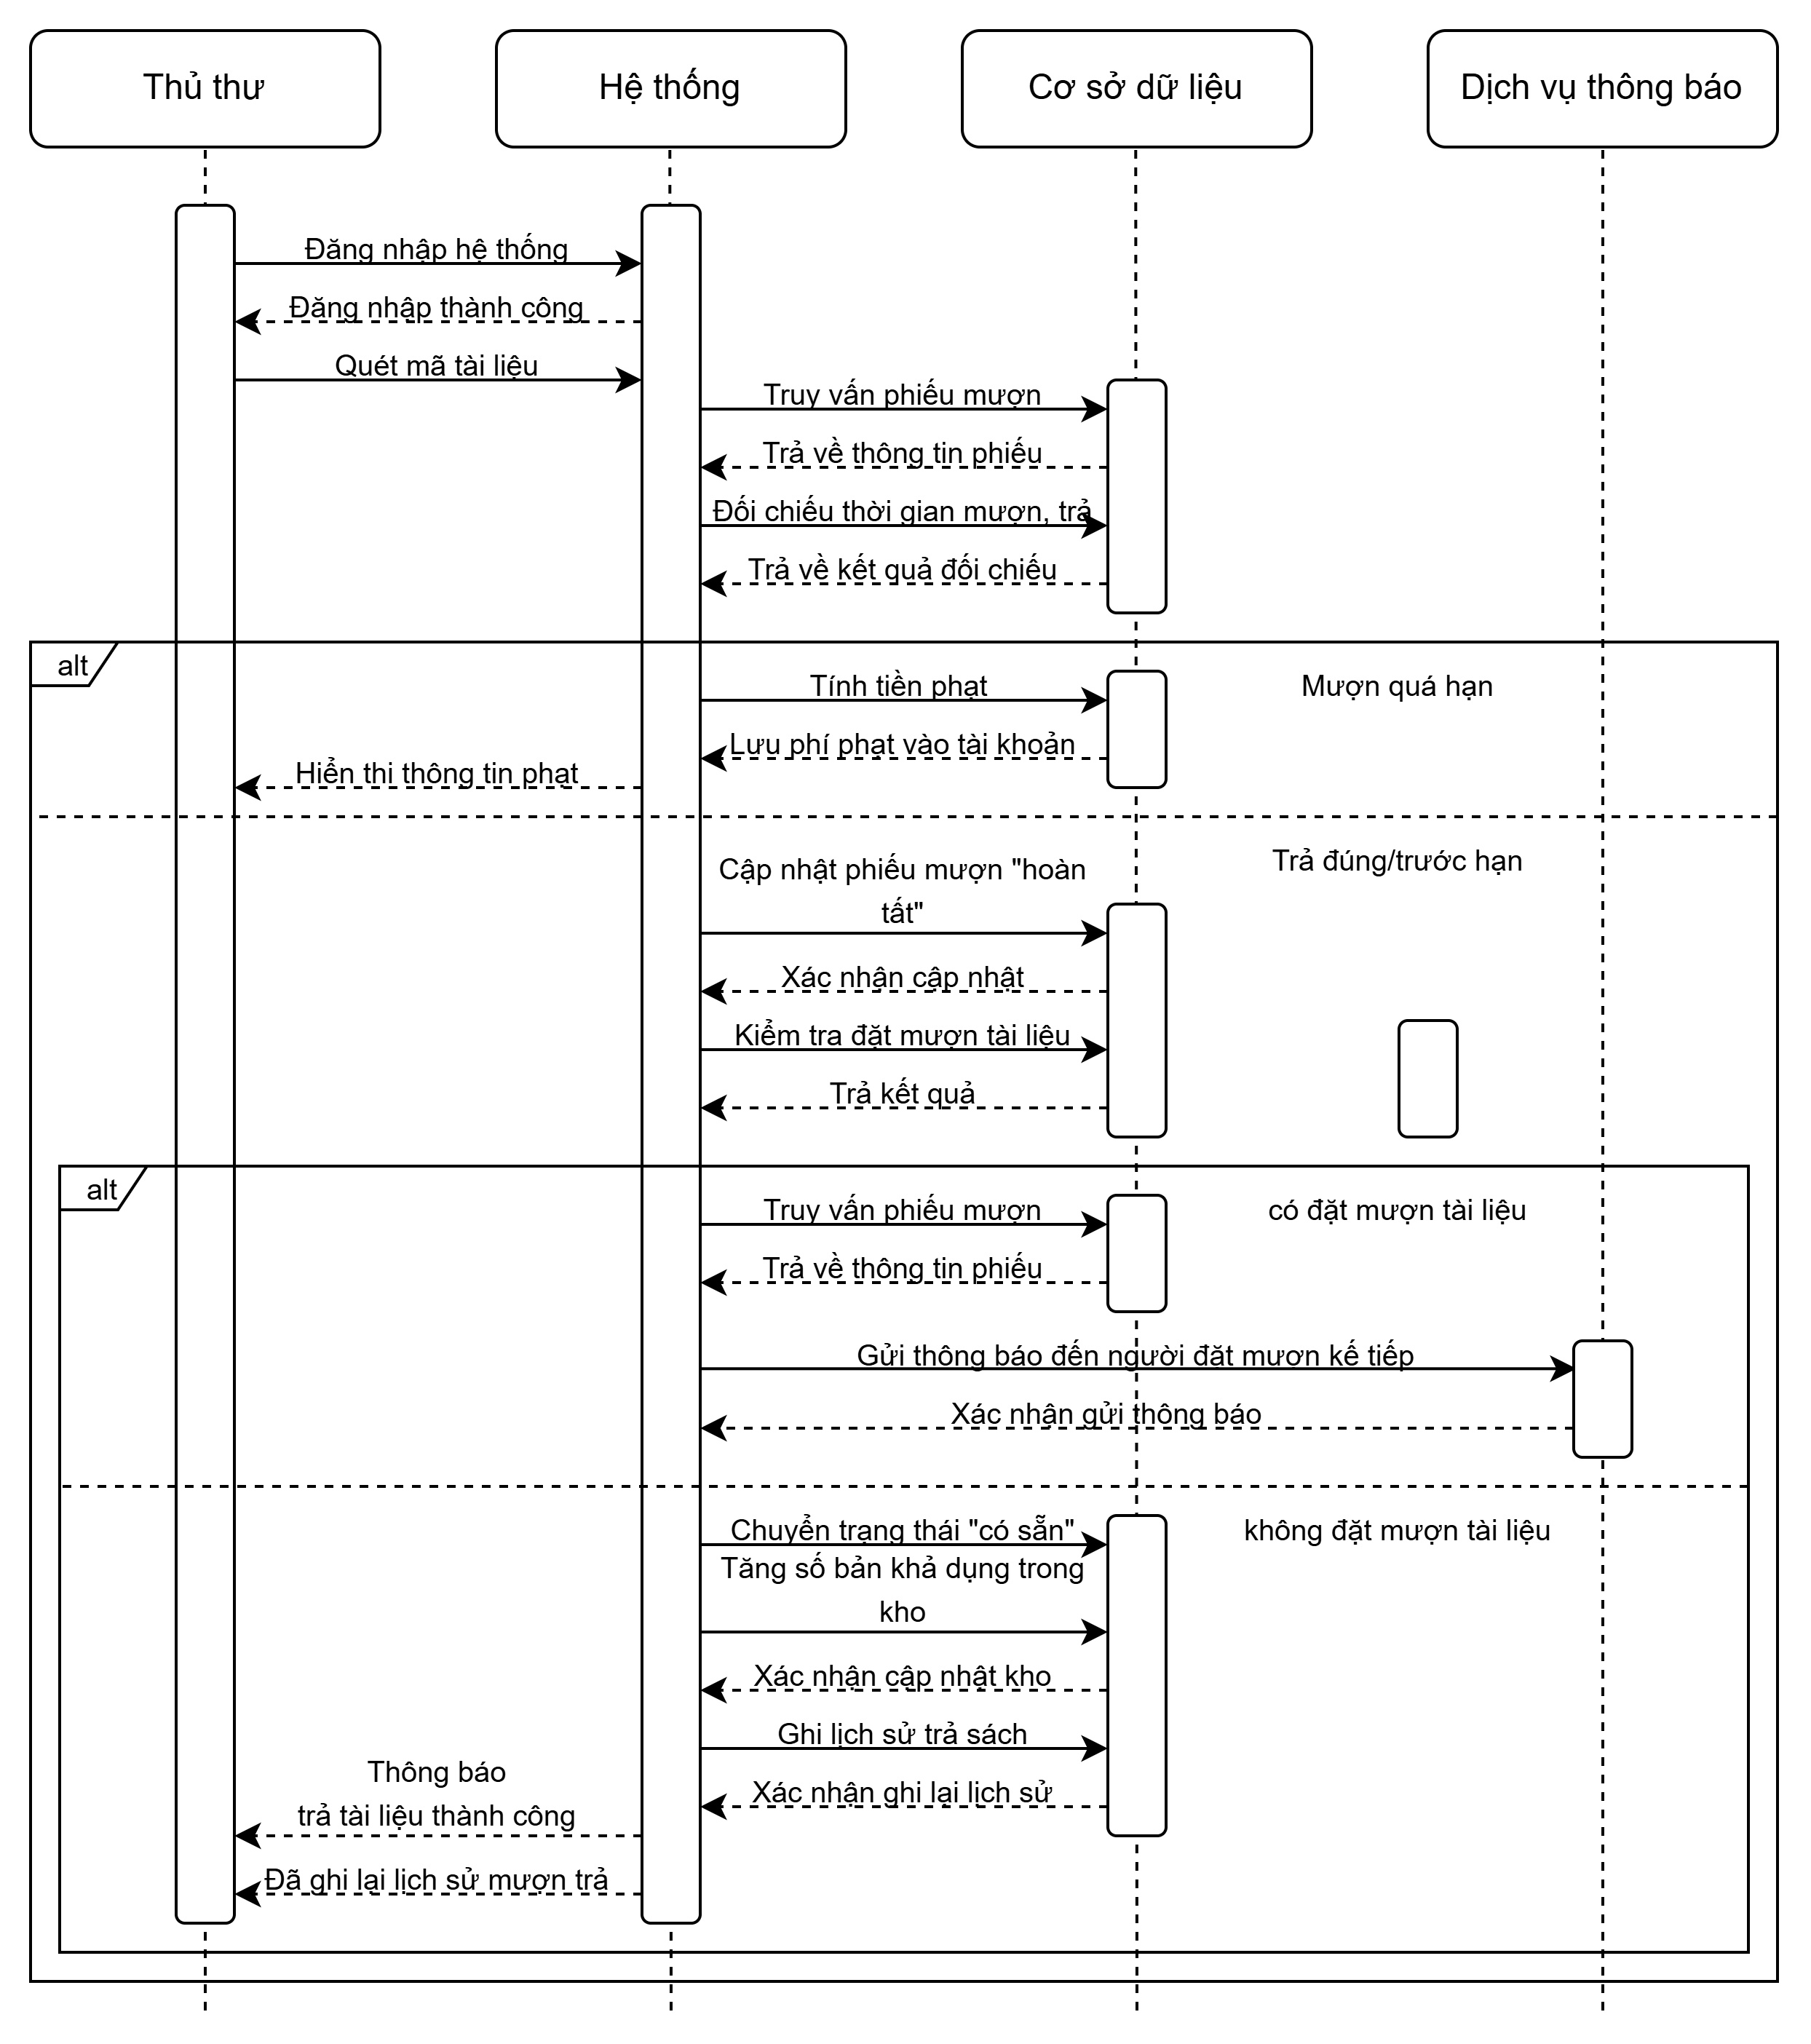
\includegraphics[width=0.6\linewidth]{Images/Seq_Tra sach.png}
    \vspace{10pt}
    \caption{Sơ đồ tuần tự Trả tài liệu}
    \label{fig:sequence_return}
\end{figure}
\begin{enumerate}
    \item Sau khi đăng nhập, khi bạn đọc đến trả tài liệu, thủ thư tiến hành truy xuất phiếu mượn từ bạn đọc và thực hiện đối chiếu thời gian trả với hạn trả.
    \begin{itemize}
        \item Nếu bạn đọc trả quá hạn, hệ thống tính bổ sung tiền phạt và cộng dồn nợ tiền phạt vào tài khoản bạn đọc trước khi tiếp tục quy trình trả tài liệu.
        \item Nếu tài liệu trả đúng hoặc sớm hạn, quy trình tiếp tục.
    \end{itemize}
    \item Hệ thống tiếp tục kiểm tra hàng chờ đặt mượn của từng tài liệu.
    \begin{itemize}
        \item Nếu hàng chờ có bạn đọc chờ mượn, hệ thống gửi thông báo cho bạn đọc kế tiếp, để trạng thái tài liệu sang "Đang chờ mượn".
        \item Nếu không có bạn đọc nào trong hàng chờ, hệ thống cộng số bản khả dụng trong kho và cập nhật kho, xác nhận "Trả tài liệu thành công".
    \end{itemize}
    Quy trình trả tài liệu kết thúc tại đây.
\end{enumerate}
\subsection{Thiết kế giao diện hệ thống}

Để trực quan hóa luồng trải nghiệm và phương thức tương tác của các tác nhân đối với hệ thống Quản lý Thư viện Trực tuyến, phần này trình bày chi tiết bản vẽ thiết kế giao diện đã được hiện thực hóa theo hướng tinh gọn và tối ưu hóa trải nghiệm người dùng.

\subsubsection{Thiết kế giao diện dành cho phân hệ Bạn đọc}

\paragraph{a) Trang chủ}
Màn hình trung tâm hiển thị ngay sau khi đăng nhập thành công, cung cấp góc nhìn tổng quan mang tính cá nhân hóa về tình trạng thẻ mượn và các tài liệu đang lưu giữ.

\begin{figure}[H]
    \centering
    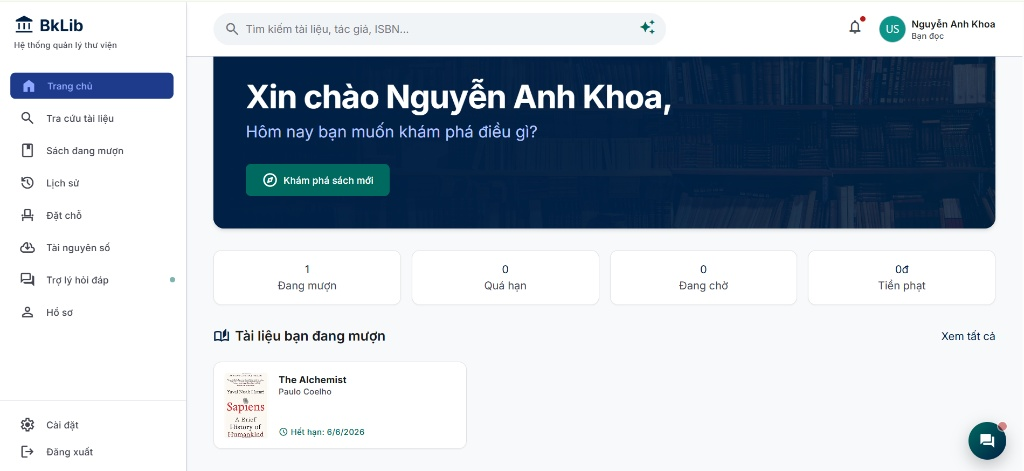
\includegraphics[width=0.95\linewidth]{Images/Reader_TrangChu.jpg}
    \vspace{10pt}
    \caption{Giao diện Trang chủ phân hệ Bạn đọc}
    \label{fig:reader_homepage}
\end{figure}

\textbf{Mô tả bố cục và thành phần giao diện:}
\begin{itemize}
    \item \textbf{Thanh điều hướng hệ thống:} Cố định bên trái, chứa liên kết điều hướng nhanh đến toàn bộ các phân hệ chức năng và lối tắt tài khoản.
    \item \textbf{Thanh công cụ trên cùng:} Tích hợp thanh tìm kiếm nhanh, trung tâm thông báo và thông tin định danh vai trò người dùng.
    \item \textbf{Hệ thống thẻ số liệu:} Khối bảng động hiển thị tổng hợp trạng thái tài khoản bao gồm số lượng sách đang mượn, sách quá hạn, sách đang chờ và tiền phạt tích lũy.
    \item \textbf{Danh sách tài liệu hiện hành:} Khu vực hiển thị danh sách các đầu sách vật lý bạn đọc đang mượn dưới dạng các thẻ thông tin trực quan.
\end{itemize}
\textbf{Các thao tác chính:} Theo dõi nhanh trạng thái nợ phạt; kiểm tra thời hạn trả sách; kích hoạt cửa sổ Trợ lý ảo hỗ trợ trực tuyến.

\paragraph{b) Trang Tra cứu tài liệu}
Giao diện phục vụ tìm kiếm thông tin thư mục và khai thác tài nguyên số trong kho thư viện.

\begin{figure}[H]
    \centering
    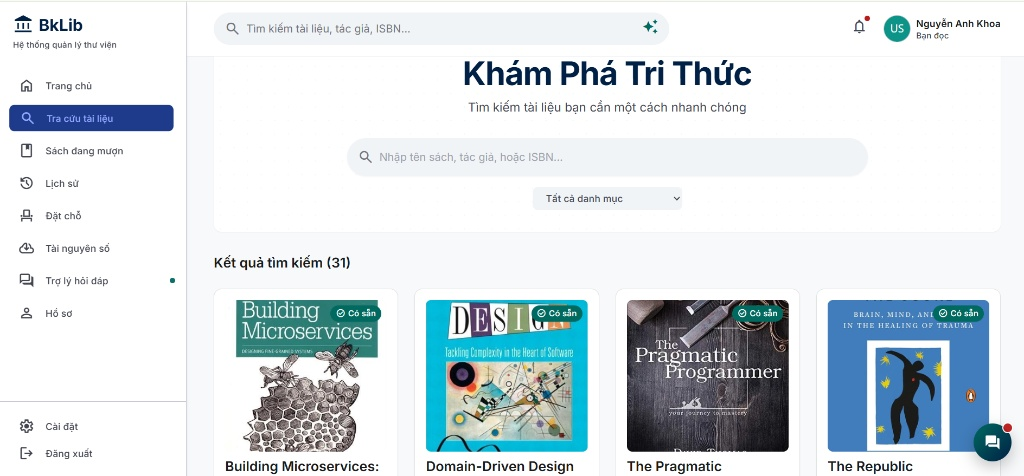
\includegraphics[width=0.95\linewidth]{Images/Reader_TraCuu.jpg}
    \vspace{10pt}
    \caption{Giao diện Trang Tra cứu tài liệu}
    \label{fig:reader_search}
\end{figure}

\textbf{Mô tả bố cục và thành phần giao diện:}
\begin{itemize}
    \item \textbf{Bộ lọc tìm kiếm trung tâm:} Gồm ô nhập từ khóa tìm kiếm nâng cao kết hợp danh mục thả xuống để phân loại nhanh theo chủ đề tài liệu.
    \item \textbf{Lưới kết quả:} Kết xuất danh sách tài liệu khớp với truy vấn dưới dạng lưới. Mỗi thẻ sách hiển thị ảnh bìa, nhãn trạng thái khả dụng, tên sách và tác giả.
\end{itemize}
\textbf{Các thao tác chính:} Tìm kiếm theo từ khóa; lọc tài liệu theo danh mục chuyên ngành; chọn thẻ sách để xem thông tin chi tiết.

\paragraph{c) Trang Quản lý Sách đang mượn}
Màn hình chuyên sâu hỗ trợ bạn đọc giám sát chu kỳ mượn trả và tương tác gia hạn tài liệu từ xa.

\begin{figure}[H]
    \centering
    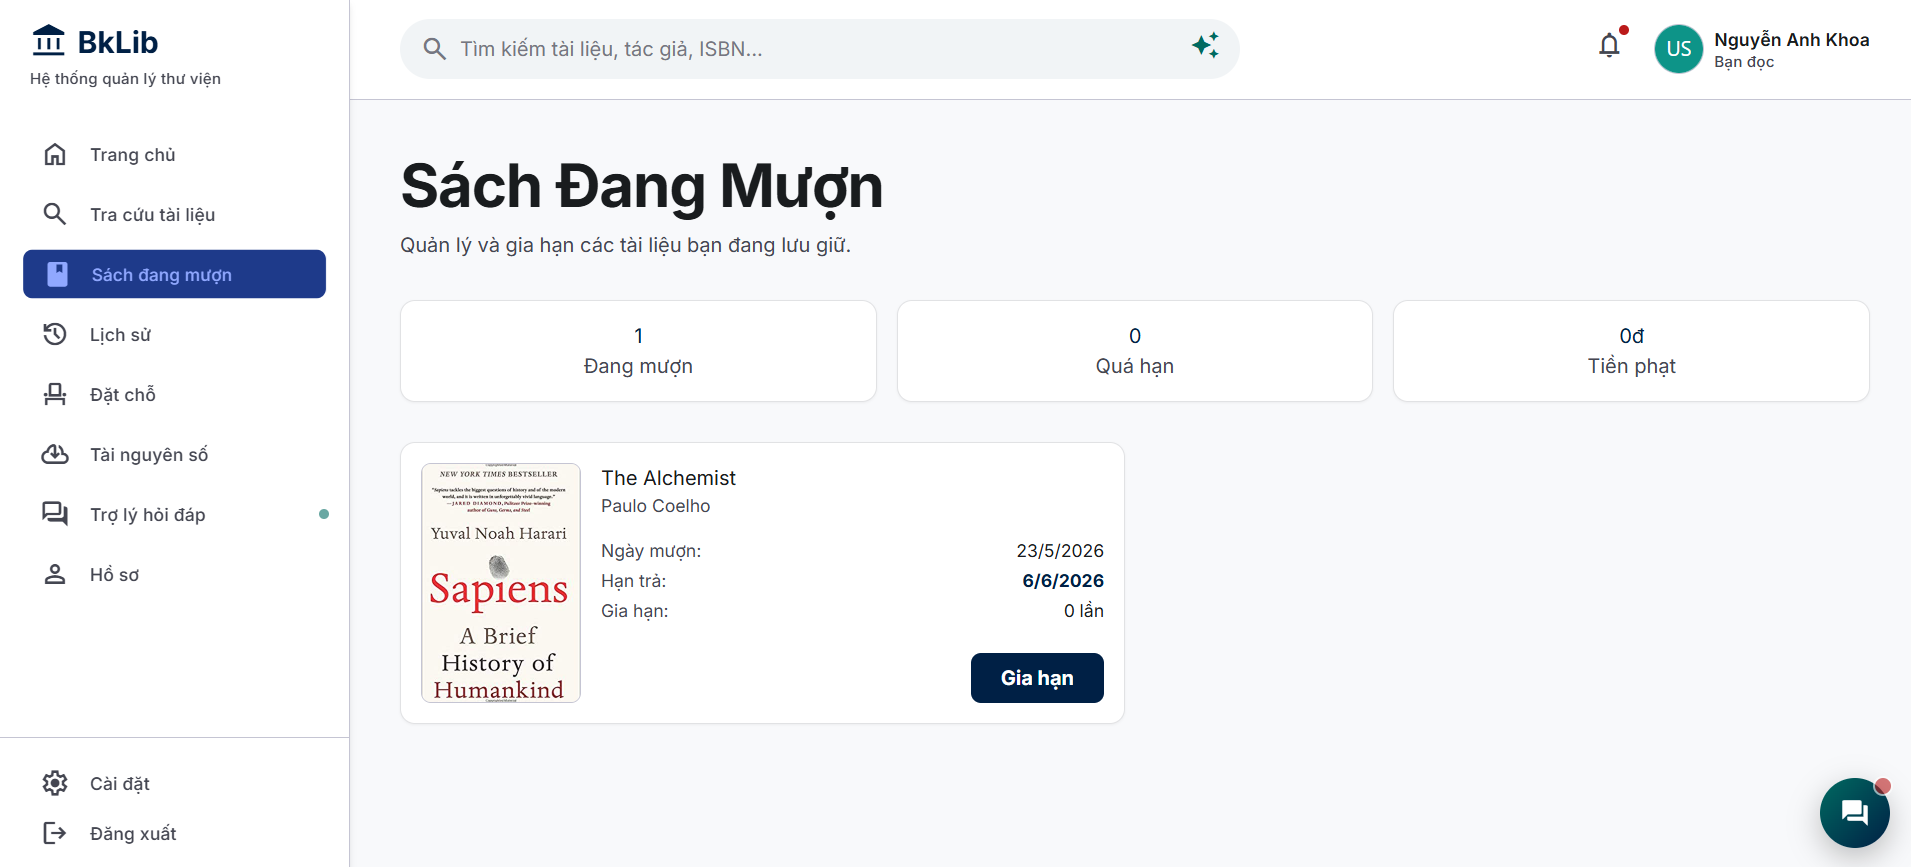
\includegraphics[width=0.95\linewidth]{Images/Reader_SachDangMuon.png}
    \vspace{10pt}
    \caption{Giao diện Trang quản lý sách đang mượn}
    \label{fig:reader_borrowing}
\end{figure}

\textbf{Mô tả bố cục và thành phần giao diện:}
\begin{itemize}
    \item \textbf{Khối chỉ số tổng hợp:} Tái hiện nhanh số lượng sách đang giữ và trạng thái vi phạm nếu có.
    \item \textbf{Danh sách thẻ mượn chi tiết:} Mỗi bản ghi hiển thị đầy đủ thông tin ngày mượn, hạn trả bắt buộc và số lần đã thực hiện gia hạn. Mỗi thẻ tích hợp sẵn nút bấm chức năng gia hạn.
\end{itemize}
\textbf{Các thao tác chính:} Theo dõi mốc thời gian hạn trả tài liệu; thực hiện lệnh gia hạn trực tuyến bất đồng bộ.

\paragraph{d) Trang Lịch sử mượn trả}
Giao diện lưu trữ nhật ký giao dịch mượn và hoàn trả tài liệu trong quá khứ của tài khoản bạn đọc.

\begin{figure}[H]
    \centering
    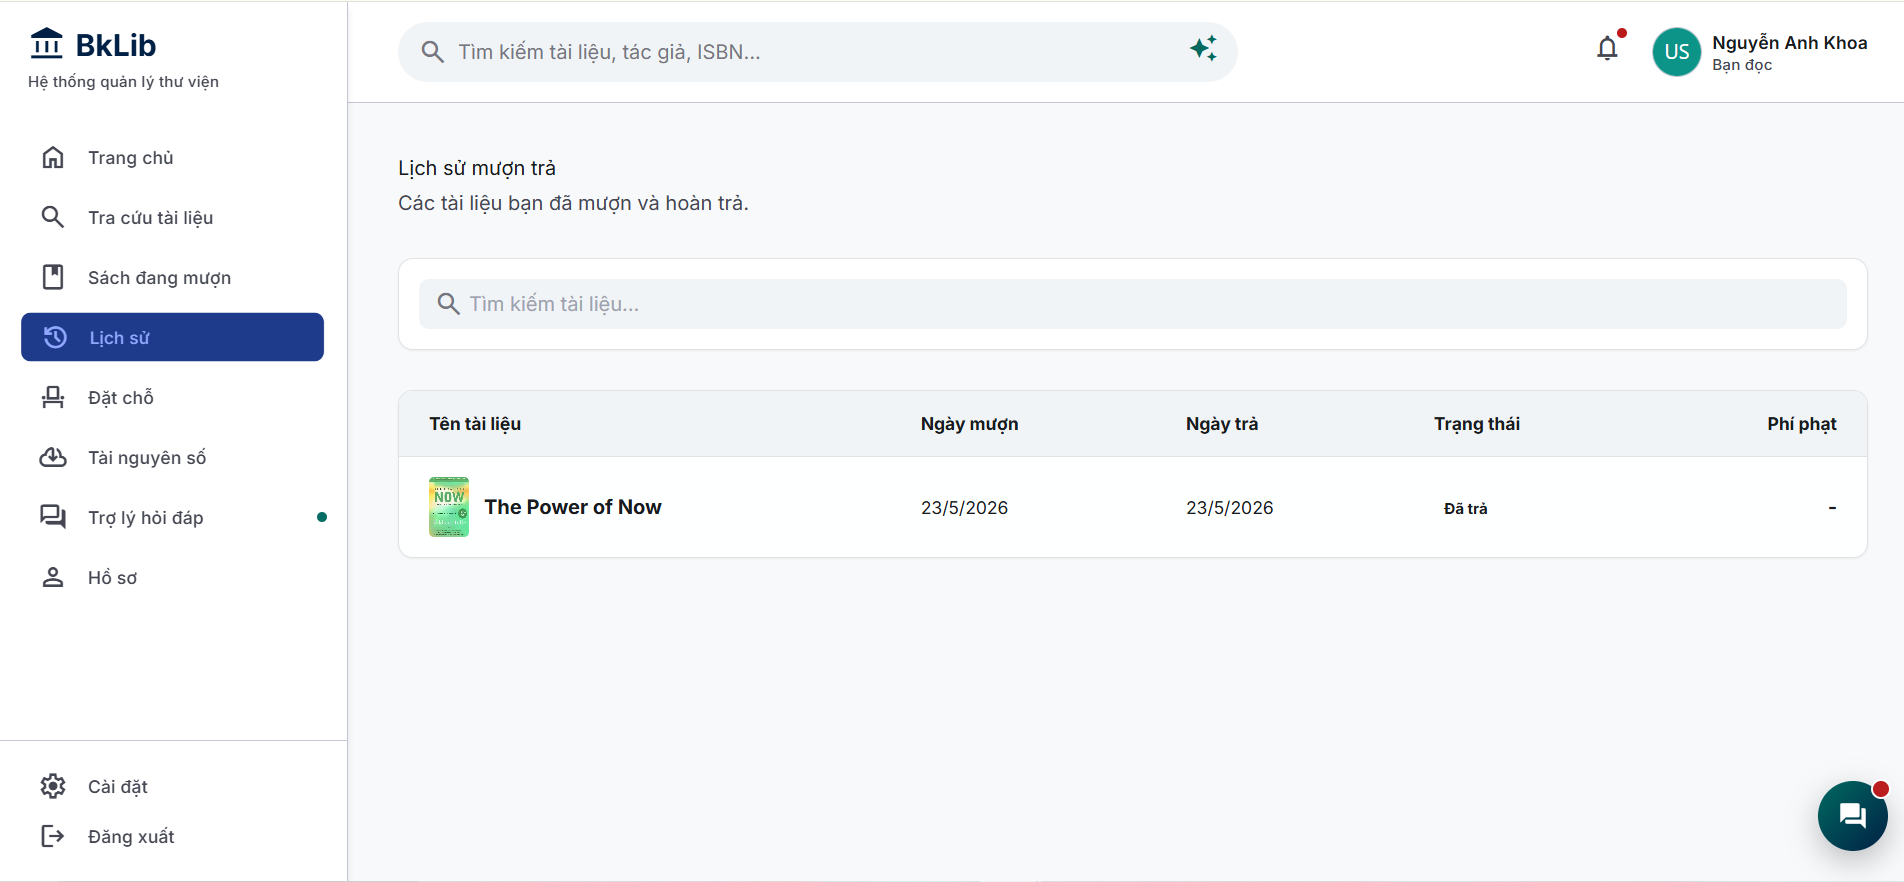
\includegraphics[width=0.95\linewidth]{Images/Reader_LichSu.png}
    \vspace{10pt}
    \caption{Giao diện Trang Lịch sử mượn trả}
    \label{fig:reader_history}
\end{figure}

\textbf{Mô tả bố cục và thành phần giao diện:} Bảng dữ liệu cấu trúc phân rõ các cột thuộc tính: Tên tài liệu, Ngày mượn, Ngày trả thực tế, Trạng thái phiếu mượn và Phí phạt phát sinh nếu có. Đầu trang tích hợp bộ lọc tìm kiếm cục bộ.

\textbf{Các thao tác chính:} Tìm kiếm và rà soát lịch sử mượn sách; đối soát thông tin phí phạt trễ hạn.

\paragraph{e) Trang Sách đang đặt giữ chỗ}
Màn hình giám sát trạng thái hàng đợi đối với các đầu sách đã hết bản khả dụng mà bạn đọc đăng ký giữ chỗ trước.

\begin{figure}[H]
    \centering
    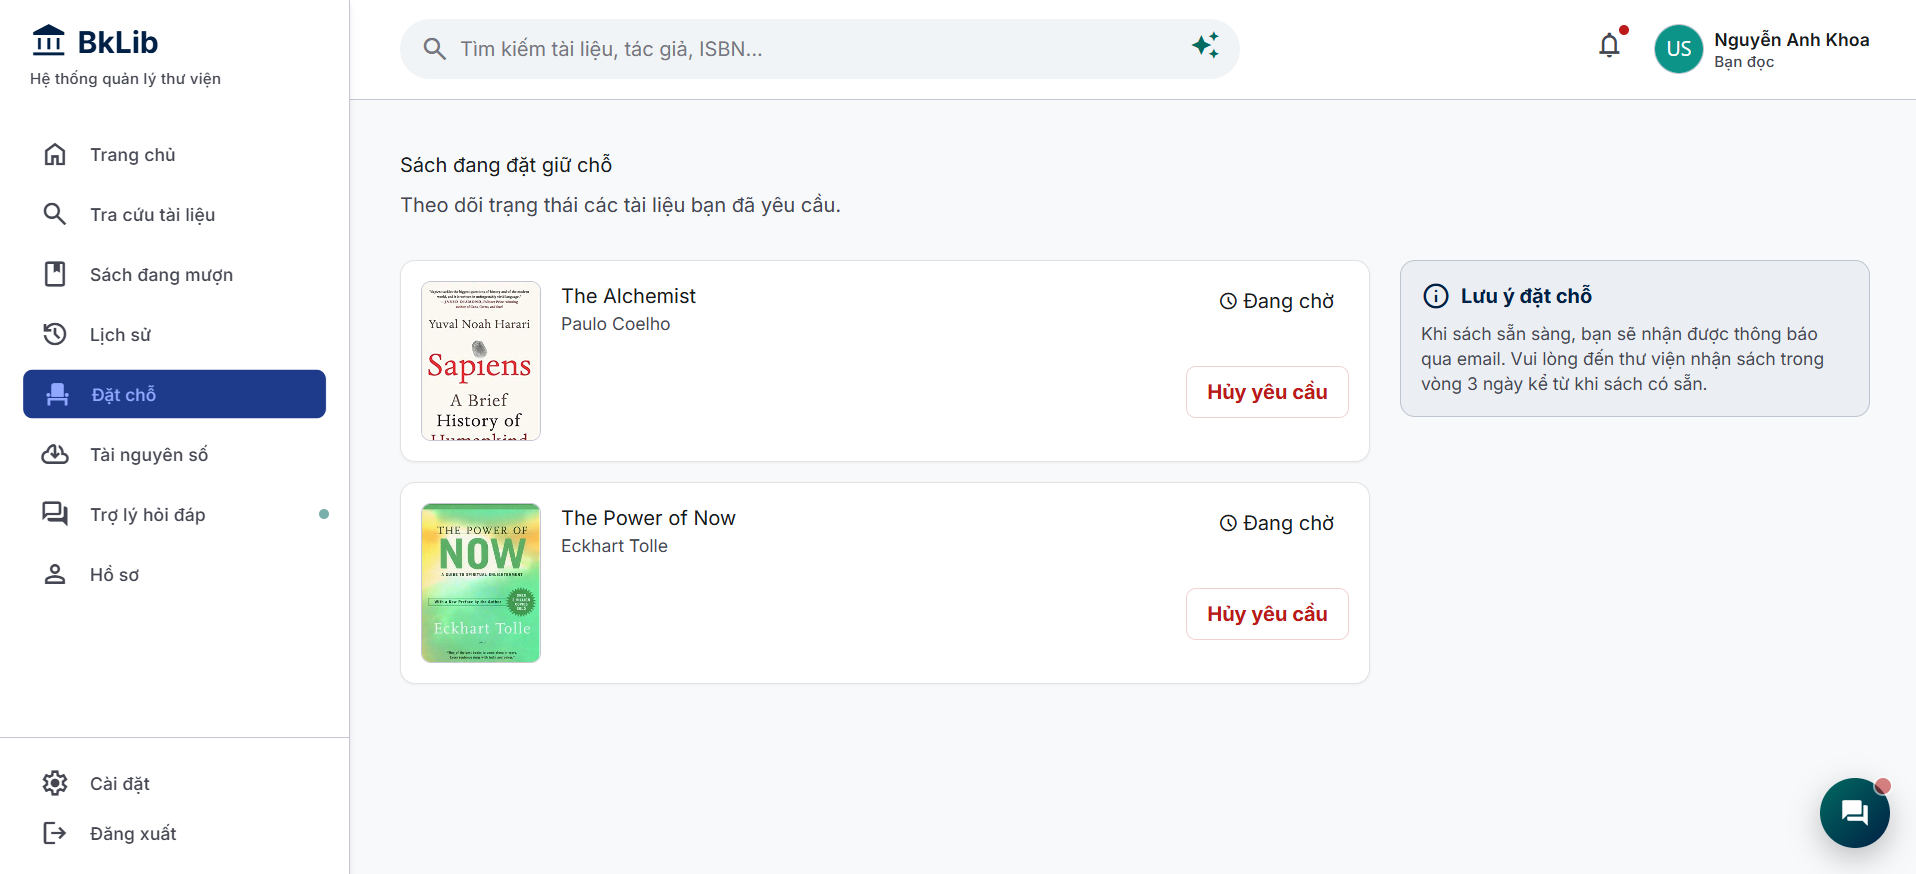
\includegraphics[width=0.95\linewidth]{Images/Reader_DatCho.png}
    \vspace{10pt}
    \caption{Giao diện Trang sách đang đặt giữ chỗ}
    \label{fig:reader_reservation}
\end{figure}

\textbf{Mô tả bố cục và thành phần giao diện:}
\begin{itemize}
    \item \textbf{Danh sách hàng đợi:} Hiển thị các tài liệu đang chờ luân chuyển kèm nút hủy yêu cầu để giải phóng vị trí xếp hàng.
    \item \textbf{Khung hướng dẫn nghiệp vụ:} Bố trí góc phải, cung cấp quy định của thư viện về thời hạn đến nhận sách khi có sẵn.
\end{itemize}
\textbf{Các thao tác chính:} Kiểm tra tiến độ xử lý yêu cầu đặt sách; chủ động hủy lệnh đặt chỗ trực tuyến.

\paragraph{f) Khung tương tác Trợ lý ảo}
Cửa sổ hội thoại thông minh hỗ trợ giải đáp tự động và tìm kiếm ngữ nghĩa theo thời gian thực cho độc giả.

\begin{figure}[H]
    \centering
    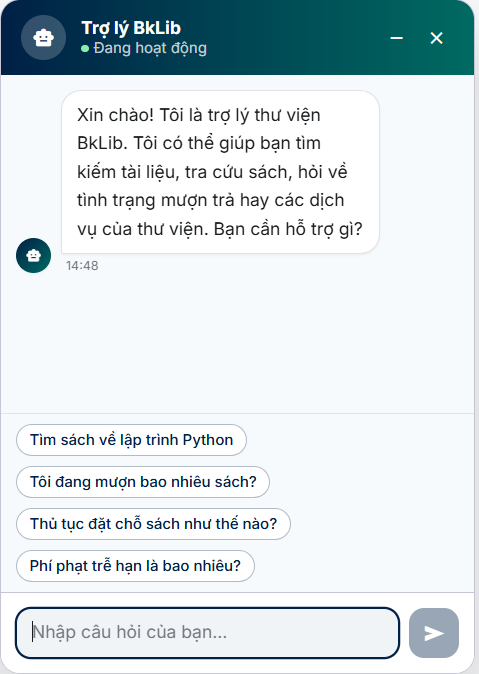
\includegraphics[width=0.45\linewidth]{Images/Reader_ChatbotAI.png}
    \vspace{10pt}
    \caption{Giao diện Khung tương tác Trợ lý ảo}
    \label{fig:reader_chatbot}
\end{figure}

\textbf{Mô tả bố cục và thành phần giao diện:} Giao diện dạng cửa sổ nhỏ gồm thanh tiêu đề hiển thị trạng thái hoạt động, luồng bong bóng trò chuyện trực quan, hệ thống các thẻ câu hỏi gợi ý nhanh và ô nhập văn bản tự nhiên.

\textbf{Các thao tác chính:} Nhập câu hỏi tự do; bấm chọn các câu hỏi mẫu có sẵn để nhận phản hồi tự động từ mô hình trí tuệ nhân tạo.

\paragraph{g) Trang Hồ sơ cá nhân \& Cài đặt}
Màn hình tích hợp cho phép bạn đọc cập nhật thông tin định danh và tùy biến cấu hình các kênh thông báo từ hệ thống.

\begin{figure}[H]
    \centering
    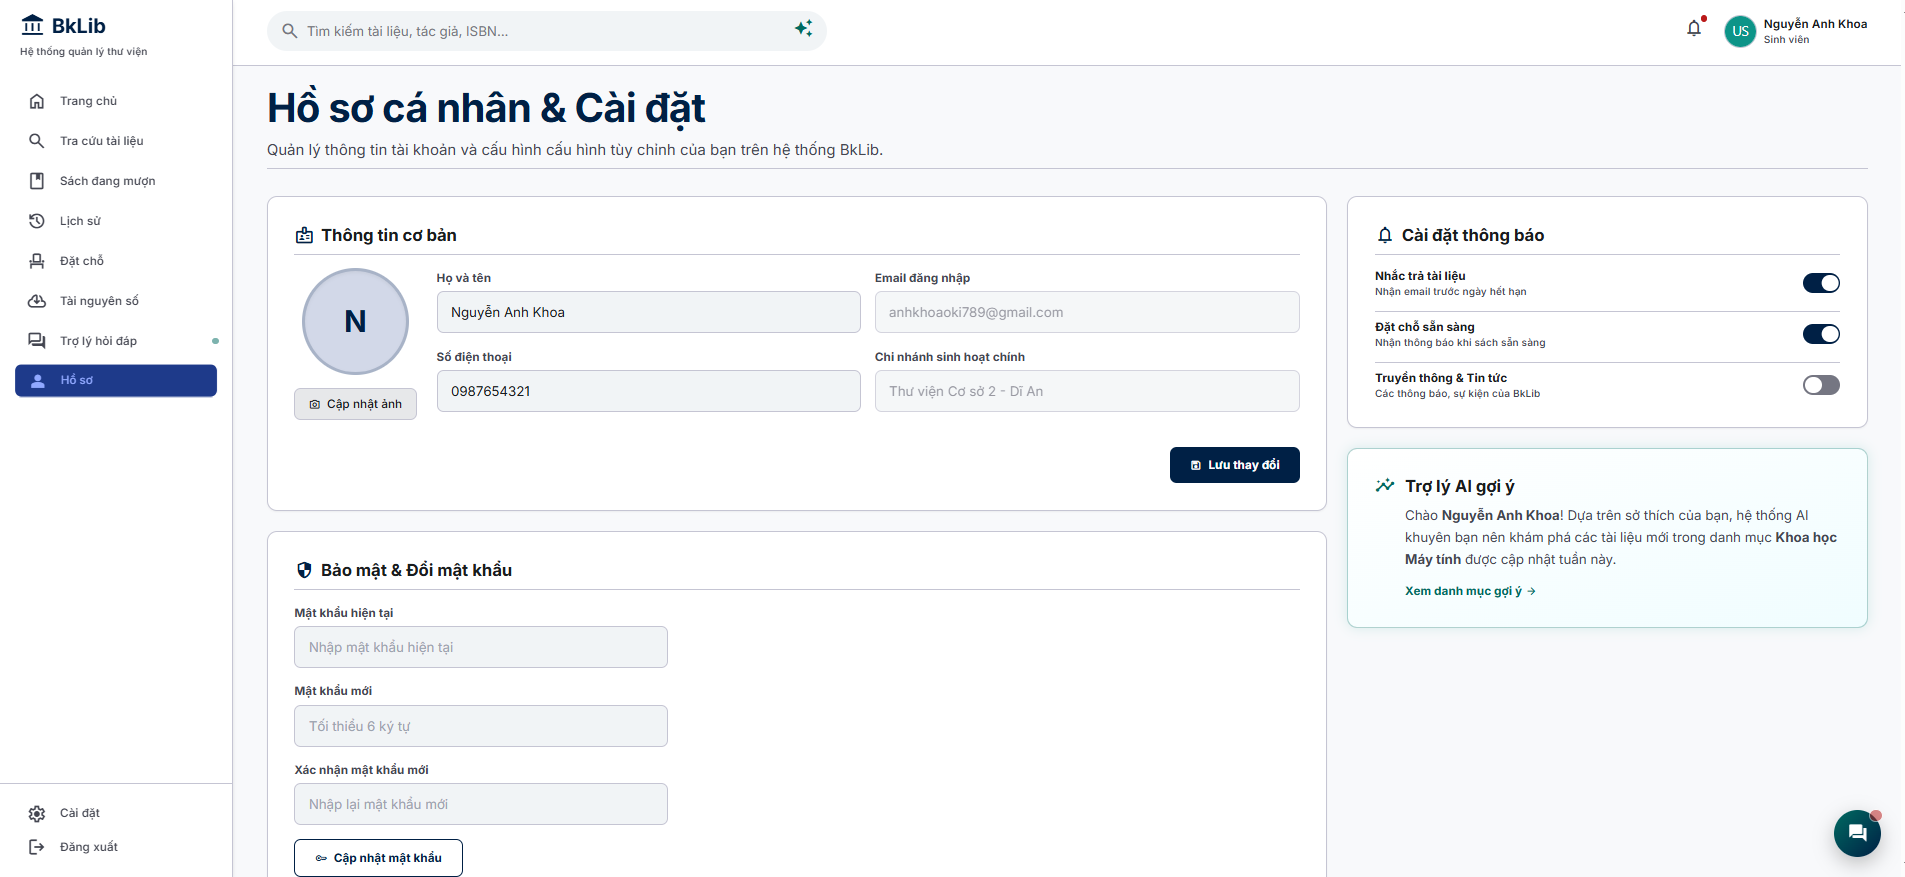
\includegraphics[width=0.95\linewidth]{Images/Reader_HoSoCaiDat.png}
    \vspace{10pt}
    \caption{Giao diện Trang Hồ sơ cá nhân và Cài đặt}
    \label{fig:reader_profile}
\end{figure}

\textbf{Mô tả bố cục và thành phần giao diện:} Thiết kế chia lưới đa phân vùng chức năng:
\begin{itemize}
    \item \textbf{Thông tin cơ bản:} Biểu mẫu cập nhật thông tin liên hệ bao gồm họ tên, số điện thoại và chi nhánh sinh hoạt.
    \item \textbf{Bảo mật:} Biểu mẫu thay đổi mật mã kiểm soát truy cập tài khoản.
    \item \textbf{Cài đặt thông báo:} Hệ thống nút gạt cấu hình nhận thông báo nhắc trả sách hoặc thông báo đặt chỗ qua thư điện tử và ứng dụng.
    \item \textbf{Hộp gợi ý:} Không gian hiển thị các đề xuất tài liệu cá nhân hóa dựa trên hành vi đọc.
\end{itemize}
\textbf{Các thao tác chính:} Thay đổi thông tin cá nhân và mật khẩu; cấu hình kênh nhận thông báo; truy cập danh mục gợi ý đọc từ hệ thống.


\subsubsection{Thiết kế giao diện dành cho phân hệ Thủ thư}

\paragraph{a) Trang chủ}
Màn hình trung tâm điều phối tác vụ hàng ngày, cung cấp các thông số vận hành tổng quan và danh sách yêu cầu cần phê duyệt trong phiên.

\begin{figure}[H]
    \centering
    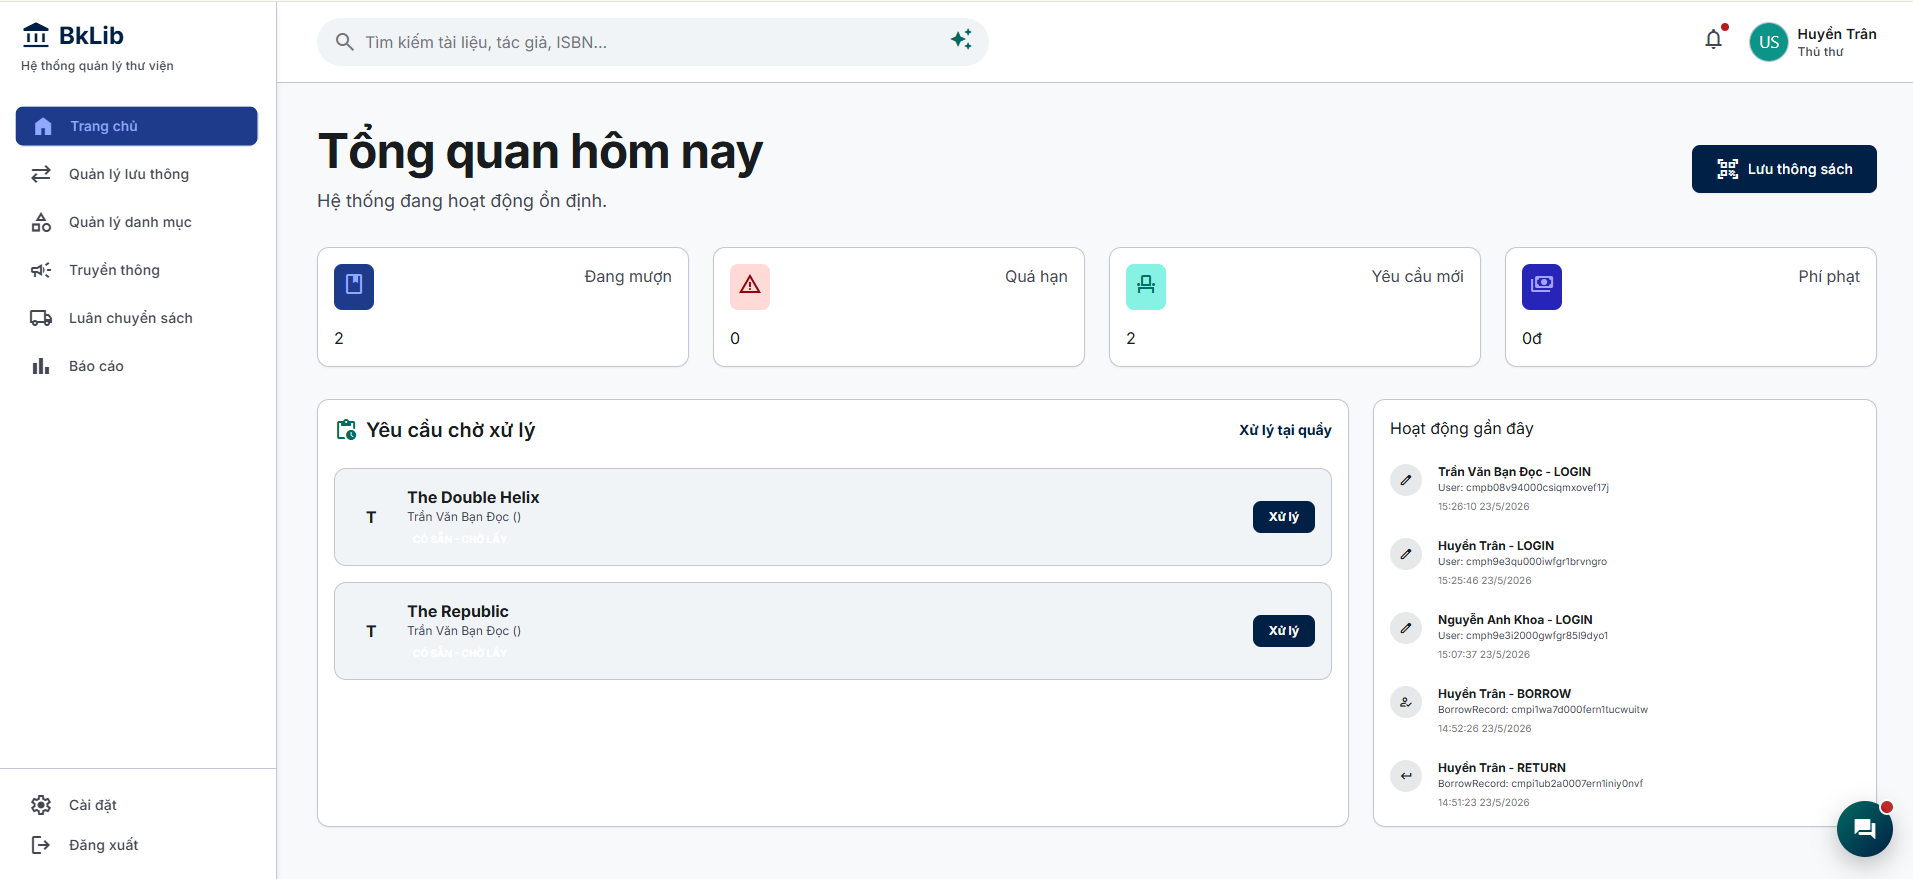
\includegraphics[width=0.95\linewidth]{Images/Librarian_TrangChu.png}
    \vspace{10pt}
    \caption{Giao diện Trang chủ phân hệ Thủ thư}
    \label{fig:librarian_homepage}
\end{figure}

\textbf{Mô tả bố cục và thành phần giao diện:}
\begin{itemize}
    \item \textbf{Thanh chức năng đặc thù:} Liên kết đến các nghiệp vụ cốt lõi bao gồm quản lý lưu thông, quản lý danh mục, truyền thông và báo cáo.
    \item \textbf{Thống kê nhanh trong ngày:} Các thẻ chỉ số đo lường khối lượng công việc hiện hành như số lượt mượn, quá hạn và yêu cầu mới.
    \item \textbf{Khối nghiệp vụ chờ xử lý:} Danh sách các yêu cầu đặt chỗ hoặc mượn trả cần thủ thư phê duyệt trực tiếp.
    \item \textbf{Nhật ký hệ thống:} Ghi vết luồng hoạt động giao dịch mượn trả thời gian thực.
\end{itemize}
\textbf{Các thao tác chính:} Kiểm soát chỉ số vận hành thư viện; tiếp nhận xử lý nhanh yêu cầu từ độc giả.

\paragraph{b) Trang Quản lý lưu thông}
Màn hình tương tác nghiệp vụ quầy hỗ trợ thủ thư xử lý luồng mượn trả và nợ phạt trực tiếp cho bạn đọc.

\begin{figure}[H]
    \centering
    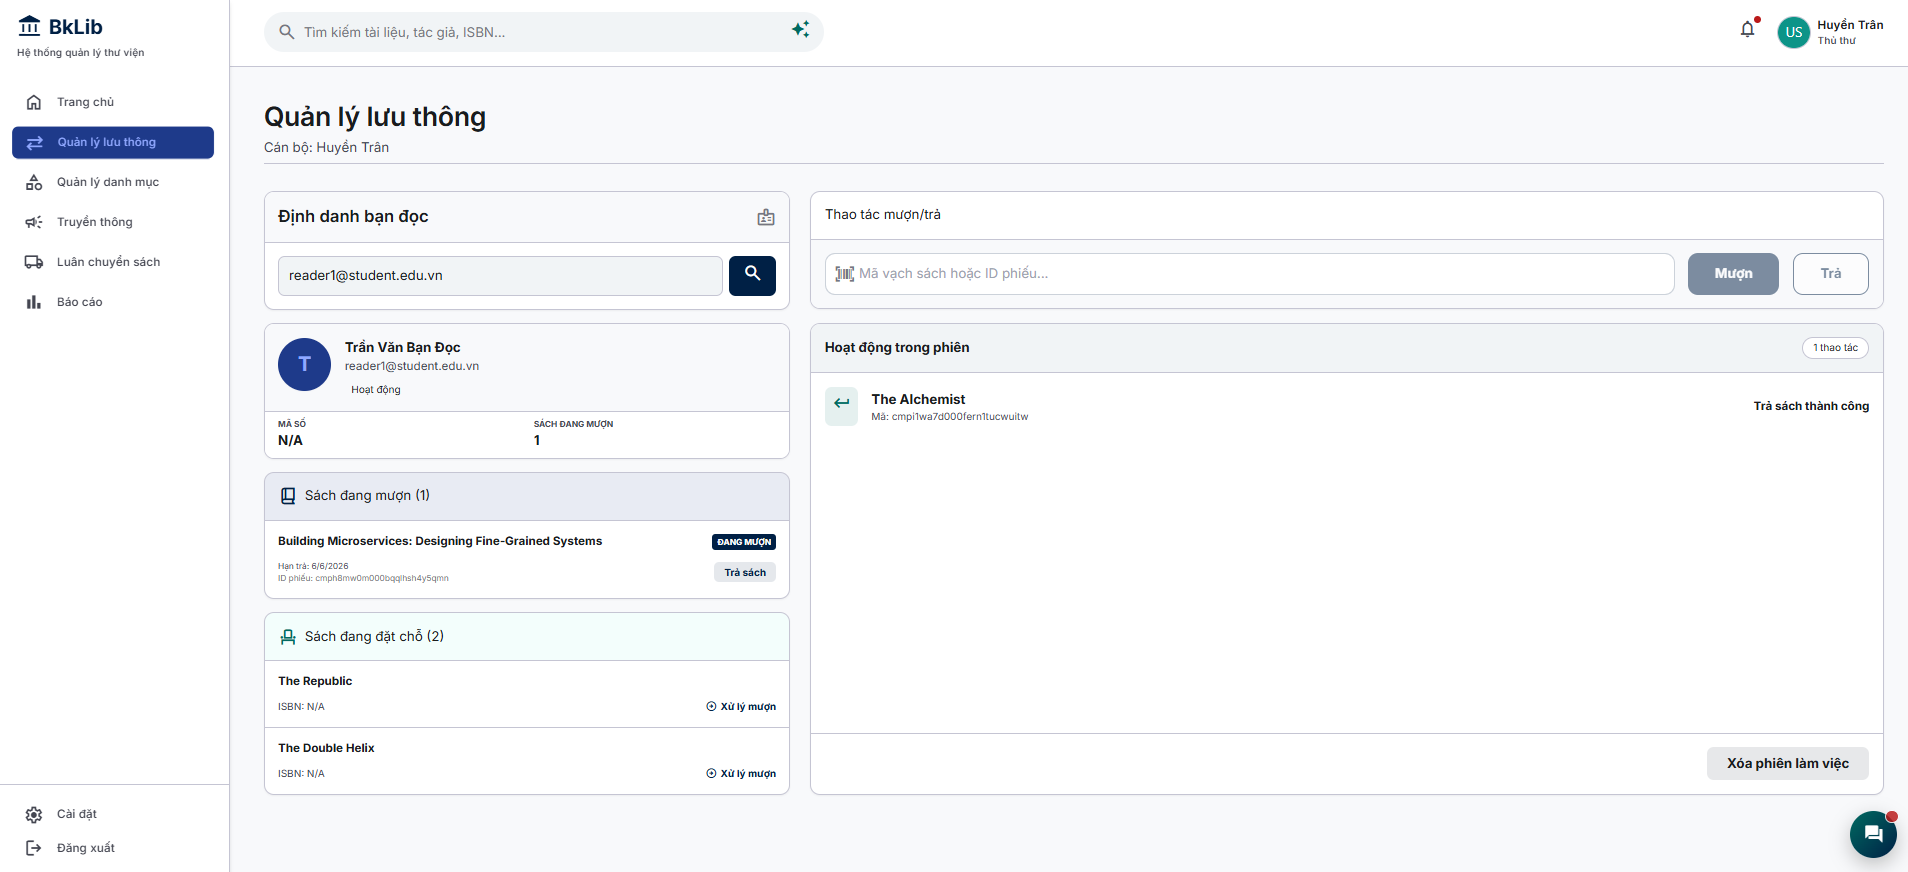
\includegraphics[width=0.95\linewidth]{Images/Librarian_QuanLyLuuThong.png}
    \vspace{10pt}
    \caption{Giao diện Trang Quản lý lưu thông tài liệu}
    \label{fig:librarian_circulation}
\end{figure}

\textbf{Mô tả bố cục và thành phần giao diện:} Bố cục chia đôi đối ứng logic:
\begin{itemize}
    \item \textbf{Bên trái:} Ô tra cứu mã thẻ hoặc thư điện tử bạn đọc; kết xuất thông tin chi tiết kèm danh sách sách đang mượn hoặc đặt chỗ của tài khoản đó.
    \item \textbf{Bên phải:} Ô nhập tiêu điểm quét mã vạch tài liệu vật lý kết hợp nút chọn chế độ hành động mượn hoặc trả và bảng hiển thị kết quả biên lai thao tác trong phiên.
\end{itemize}
\textbf{Các thao tác chính:} Tra cứu hồ sơ bạn đọc tại quầy; quét mã vạch thực hiện giao dịch mượn hoặc trả sách; xử lý thu hồi tài liệu nhanh.

\paragraph{c) Trang Quản lý danh mục tài liệu}
Giao diện quản lý các biểu ghi thư mục và các bản sao vật lý trong kho thư viện.

\begin{figure}[H]
    \centering
    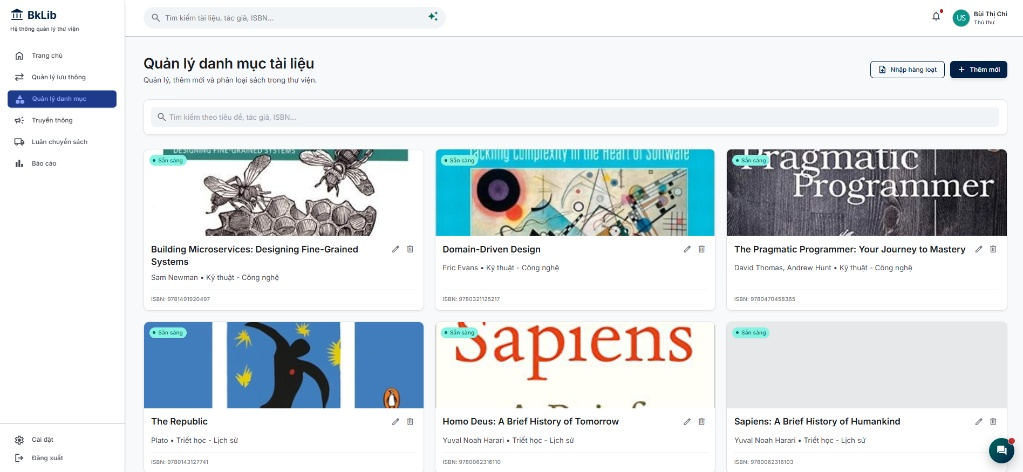
\includegraphics[width=0.95\linewidth]{Images/Librarian_QuanLyDanhMuc.jpg}
    \vspace{10pt}
    \caption{Giao diện Trang Quản lý danh mục tài liệu}
    \label{fig:librarian_catalog}
\end{figure}

\textbf{Mô tả bố cục và thành phần giao diện:}
\begin{itemize}
    \item \textbf{Thanh tác vụ đầu trang:} Tích hợp công cụ tìm kiếm sách theo từ khóa hoặc mã số tiêu chuẩn, nút nhập liệu hàng loạt và nút thêm mới tài liệu.
    \item \textbf{Lưới quản lý danh mục:} Hiển thị danh mục sách phân trang. Trên mỗi thẻ sách tích hợp sẵn hai công cụ hành động là chỉnh sửa thuộc tính và xóa biểu ghi.
\end{itemize}
\textbf{Các thao tác chính:} Tìm kiếm biên mục sách; kích hoạt biểu mẫu thêm, sửa hoặc xóa thông tin tài liệu.

\paragraph{d) Trang Quản lý truyền thông}
Phân hệ hỗ trợ thủ thư biên soạn nội dung và phân phối thông báo hệ thống đến các nhóm đối tượng độc giả.

\begin{figure}[H]
    \centering
    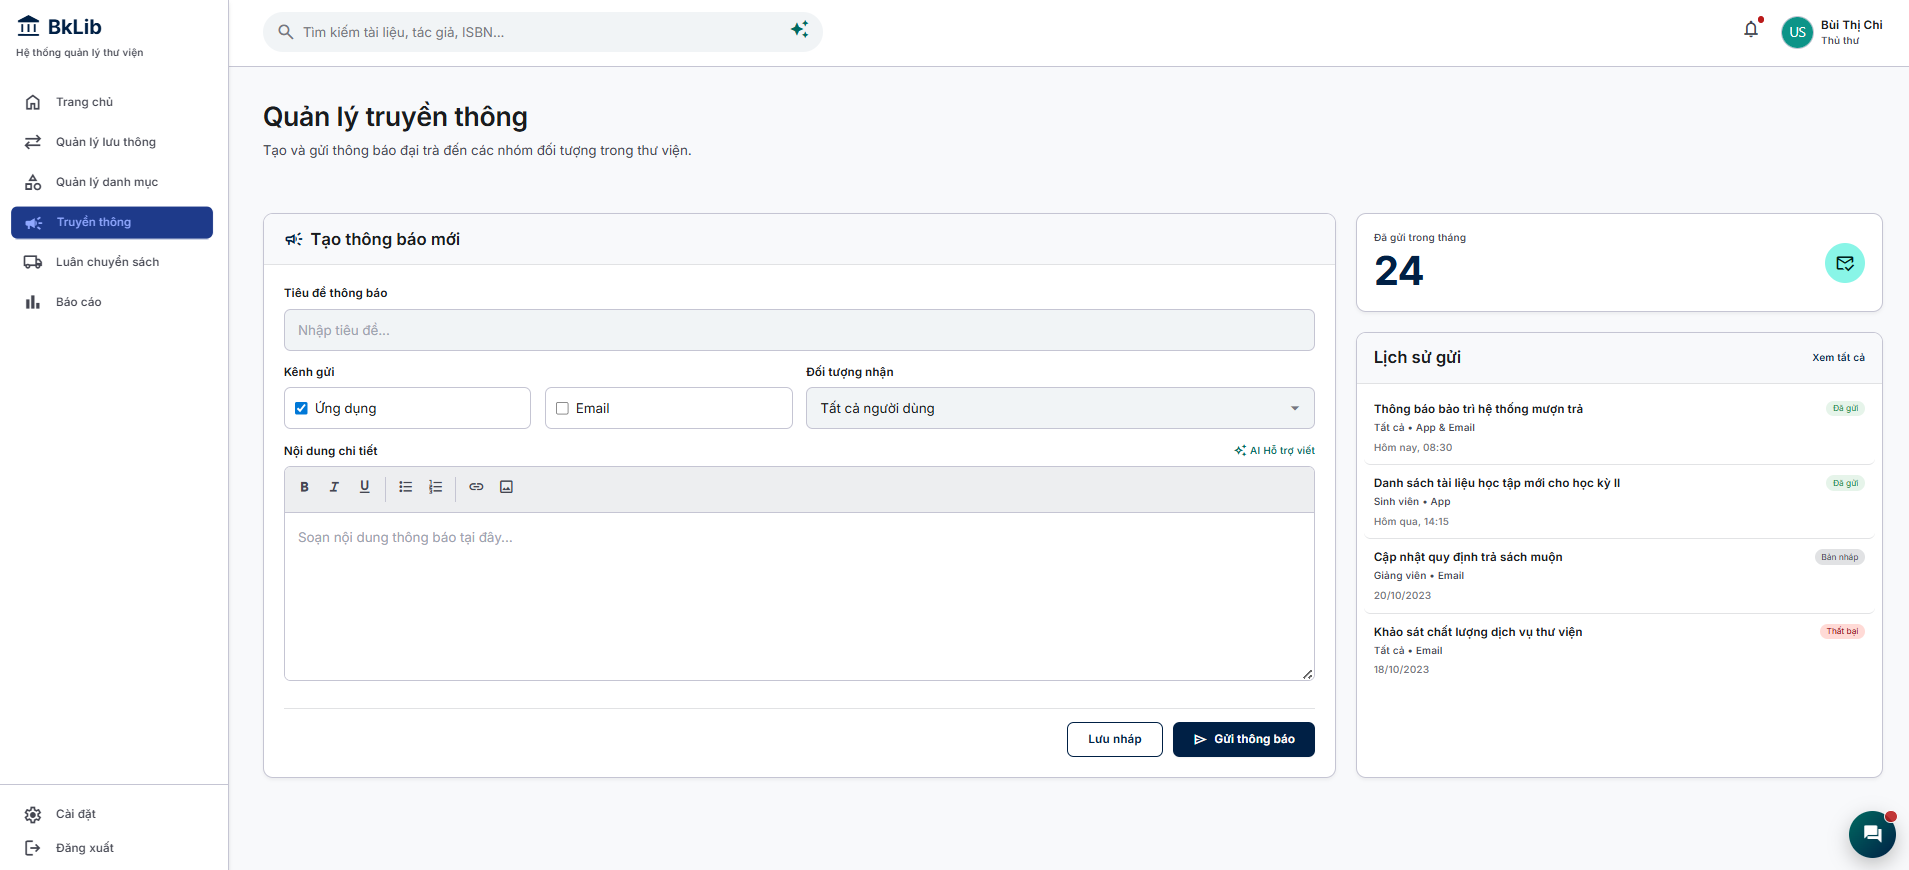
\includegraphics[width=0.95\linewidth]{Images/Librarian_TruyenThong.png}
    \vspace{10pt}
    \caption{Giao diện Trang Quản lý truyền thông}
    \label{fig:librarian_notification}
\end{figure}

\textbf{Mô tả bố cục và thành phần giao diện:}
\begin{itemize}
    \item \textbf{Vùng soạn thảo:} Biểu mẫu cấu hình thông báo gồm tiêu đề, lựa chọn kênh gửi, phân loại đối tượng nhận và trình soạn thảo văn bản định dạng nâng cao.
    \item \textbf{Vùng lịch sử:} Biểu đồ thống kê số lượng tin nhắn và danh bạ nhật ký lưu vết trạng thái các thông báo đã phát hành trong quá khứ.
\end{itemize}
\textbf{Các thao tác chính:} Soạn thảo thông báo mới; cấu hình nhóm đích nhận tin; kiểm tra lịch sử gửi tin.

\paragraph{e) Trang Báo cáo \& Thống kê}
Màn hình tổng hợp và trực quan hóa toàn bộ dữ liệu hoạt động của thư viện phục vụ công tác quản lý chuyên sâu.

\begin{figure}[H]
    \centering
    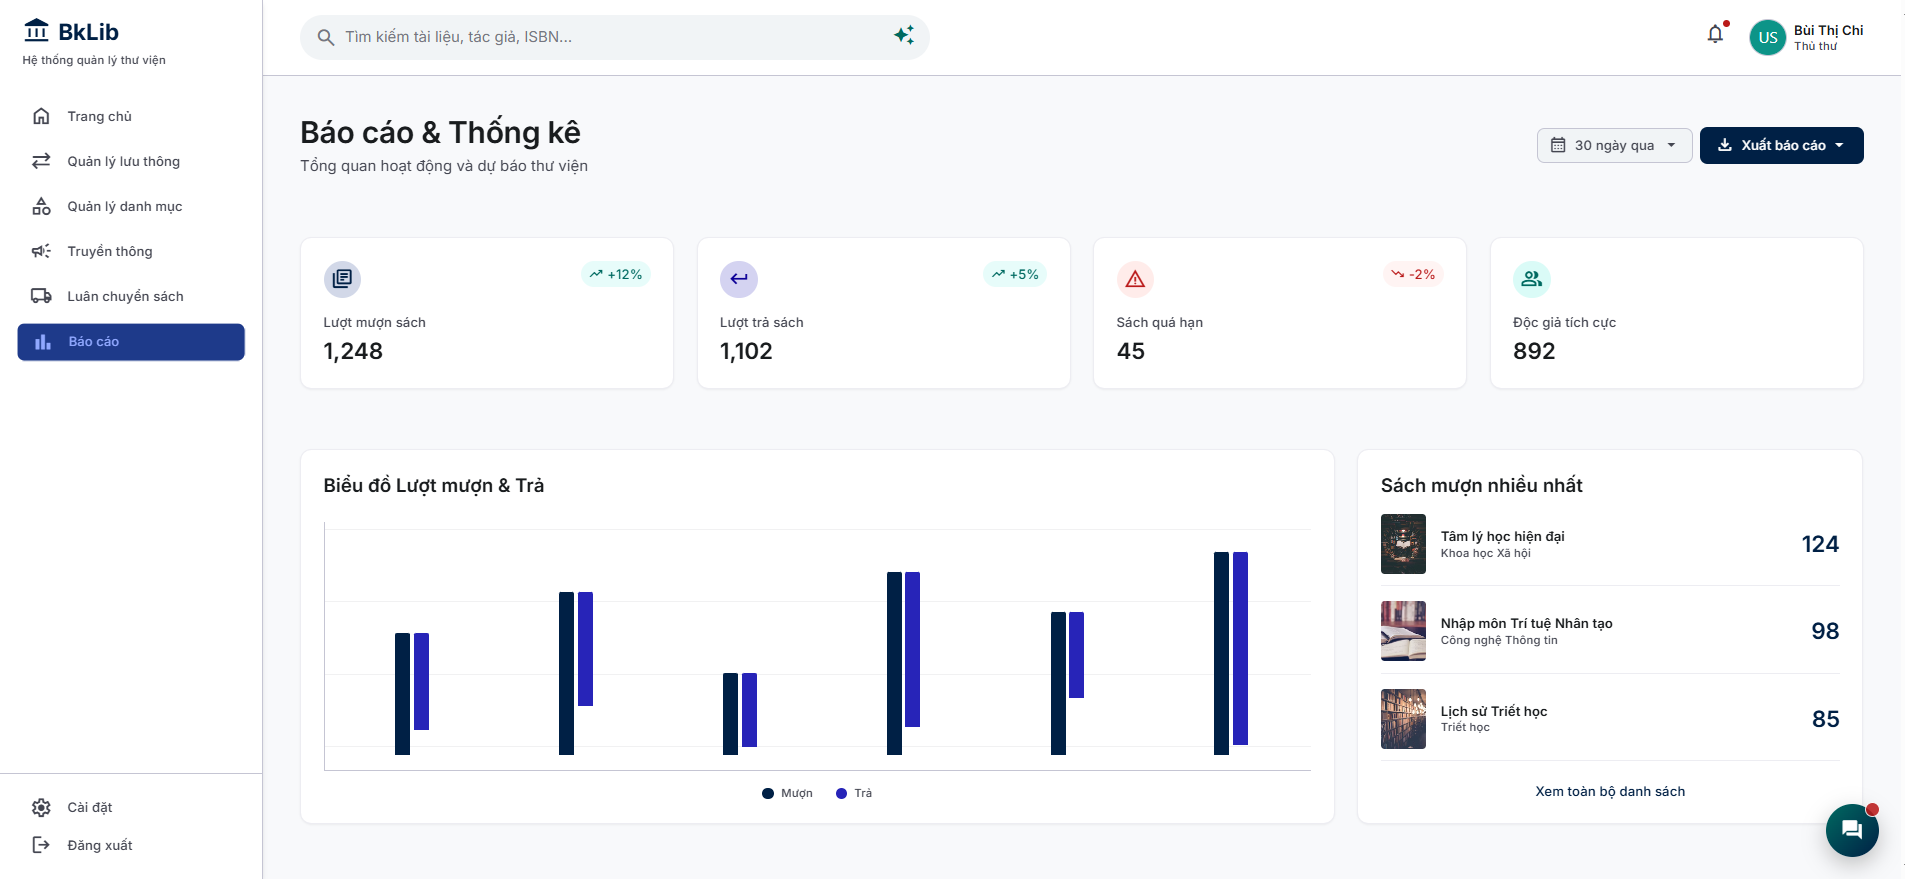
\includegraphics[width=0.95\linewidth]{Images/Librarian_BaoCao.png}
    \vspace{10pt}
    \caption{Giao diện Trang Báo cáo và Thống kê dành cho Thủ thư}
    \label{fig:librarian_report}
\end{figure}

\textbf{Mô tả bố cục và thành phần giao diện:}
\begin{itemize}
    \item \textbf{Bộ lọc và Xuất bản:} Công cụ giới hạn phạm vi thời gian thống kê dữ liệu và lối tắt xuất tệp báo cáo định dạng bảng tính hoặc tài liệu di động.
    \item \textbf{Bảng chỉ số hiệu năng:} Các khối số liệu đo lường tần suất mượn, trả, tỷ lệ trễ hạn kèm biểu đồ cột trực quan hóa xu hướng biến động theo thời gian.
    \item \textbf{Bảng xếp hạng lưu thông:} Danh sách các đầu sách có tần suất mượn cao nhất hệ thống.
\end{itemize}
\textbf{Các thao tác chính:} Lọc dữ liệu thống kê theo chu kỳ; trích xuất file báo cáo phục vụ quản trị; phân tích xu hướng khai thác tài liệu của thư viện.
\subsubsection{Thiết kế giao diện dành cho Quản trị viên }

\paragraph{a) Trang chủ (Tổng quan hệ thống)}
Màn hình trung tâm giúp quản trị viên giám sát toàn diện hiệu năng phần cứng, lưu lượng lưu trữ đám mây và trạng thái hoạt động tổng quát của hệ thống.

\begin{figure}[H]
    \centering
    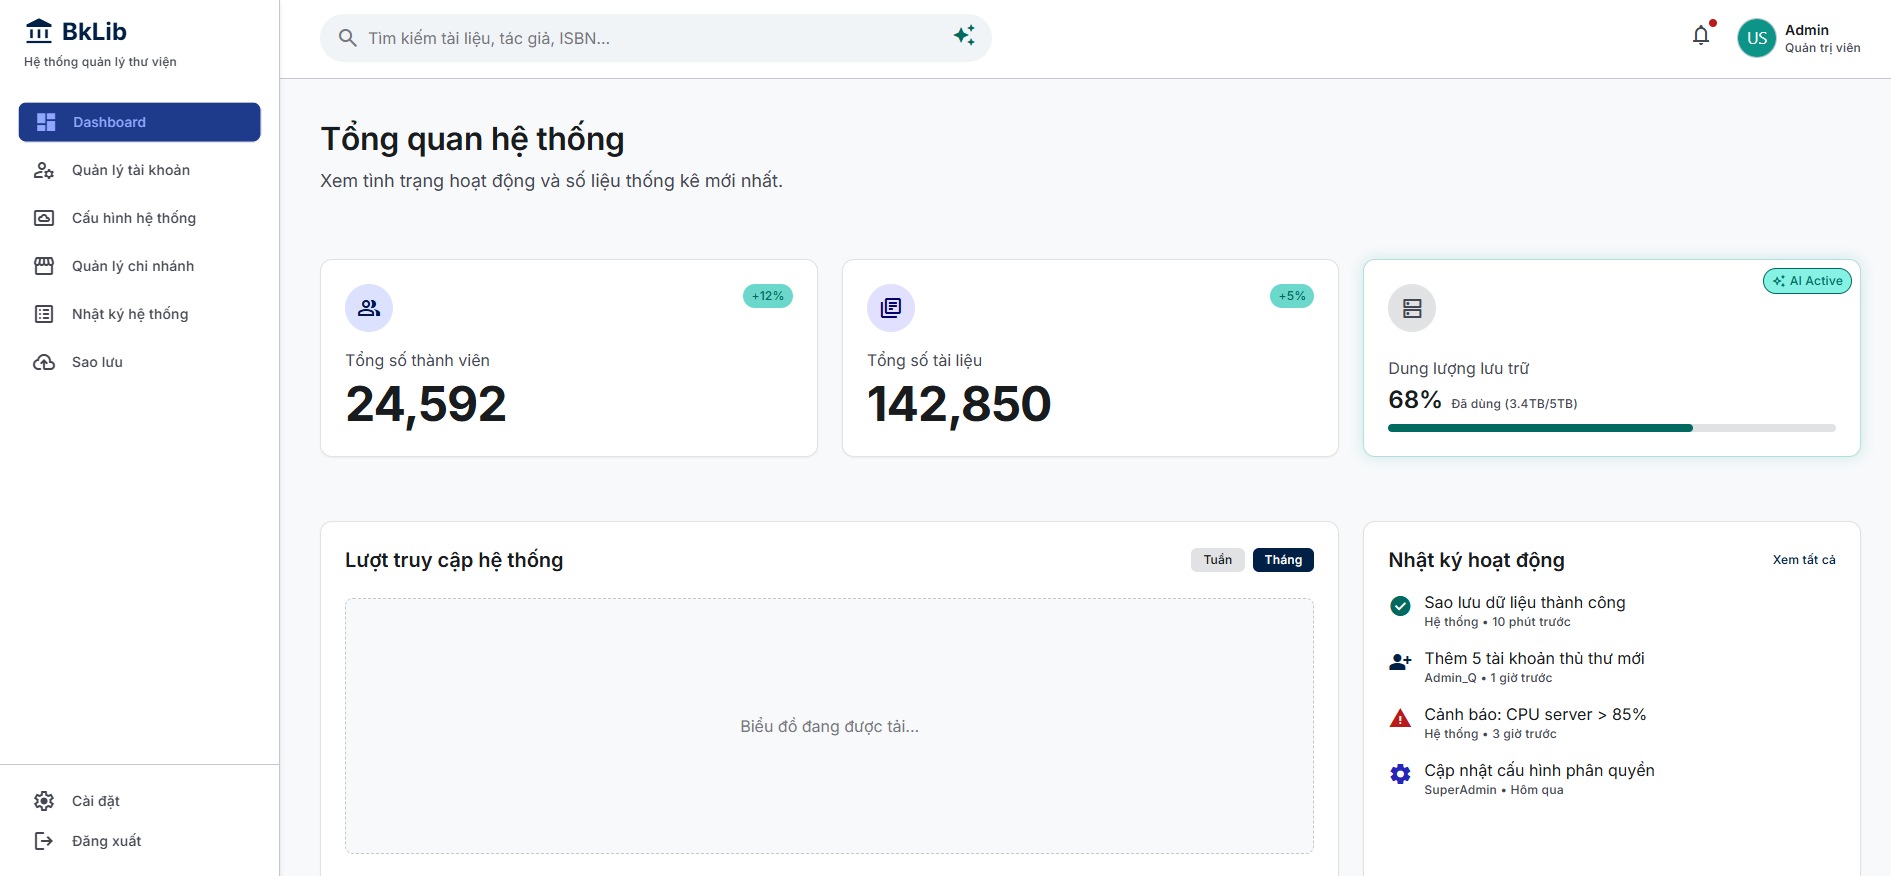
\includegraphics[width=0.95\linewidth]{Images/Admin_Dashboard.png}
    \vspace{10pt}
    \caption{Giao diện Trang tổng quan hệ thống của Quản trị viên}
    \label{fig:admin_dashboard}
\end{figure}

\textbf{Mô tả chức năng giao diện:} Hiển thị các thẻ chỉ số đo lường quy mô thực tế (tổng số thành viên, tổng số tài liệu) và tiến độ sử dụng dung lượng lưu trữ đám mây. Đồng thời kết xuất biểu đồ giám sát lượt truy cập và bảng luồng nhật ký hoạt động, cảnh báo an ninh hạ tầng phần cứng theo thời gian thực.

\paragraph{b) Trang Quản lý tài khoản người dùng}
Màn hình phân quyền và kiểm soát trạng thái hoạt động của toàn bộ các tài khoản định danh tham gia vào hệ thống.

\begin{figure}[H]
    \centering
    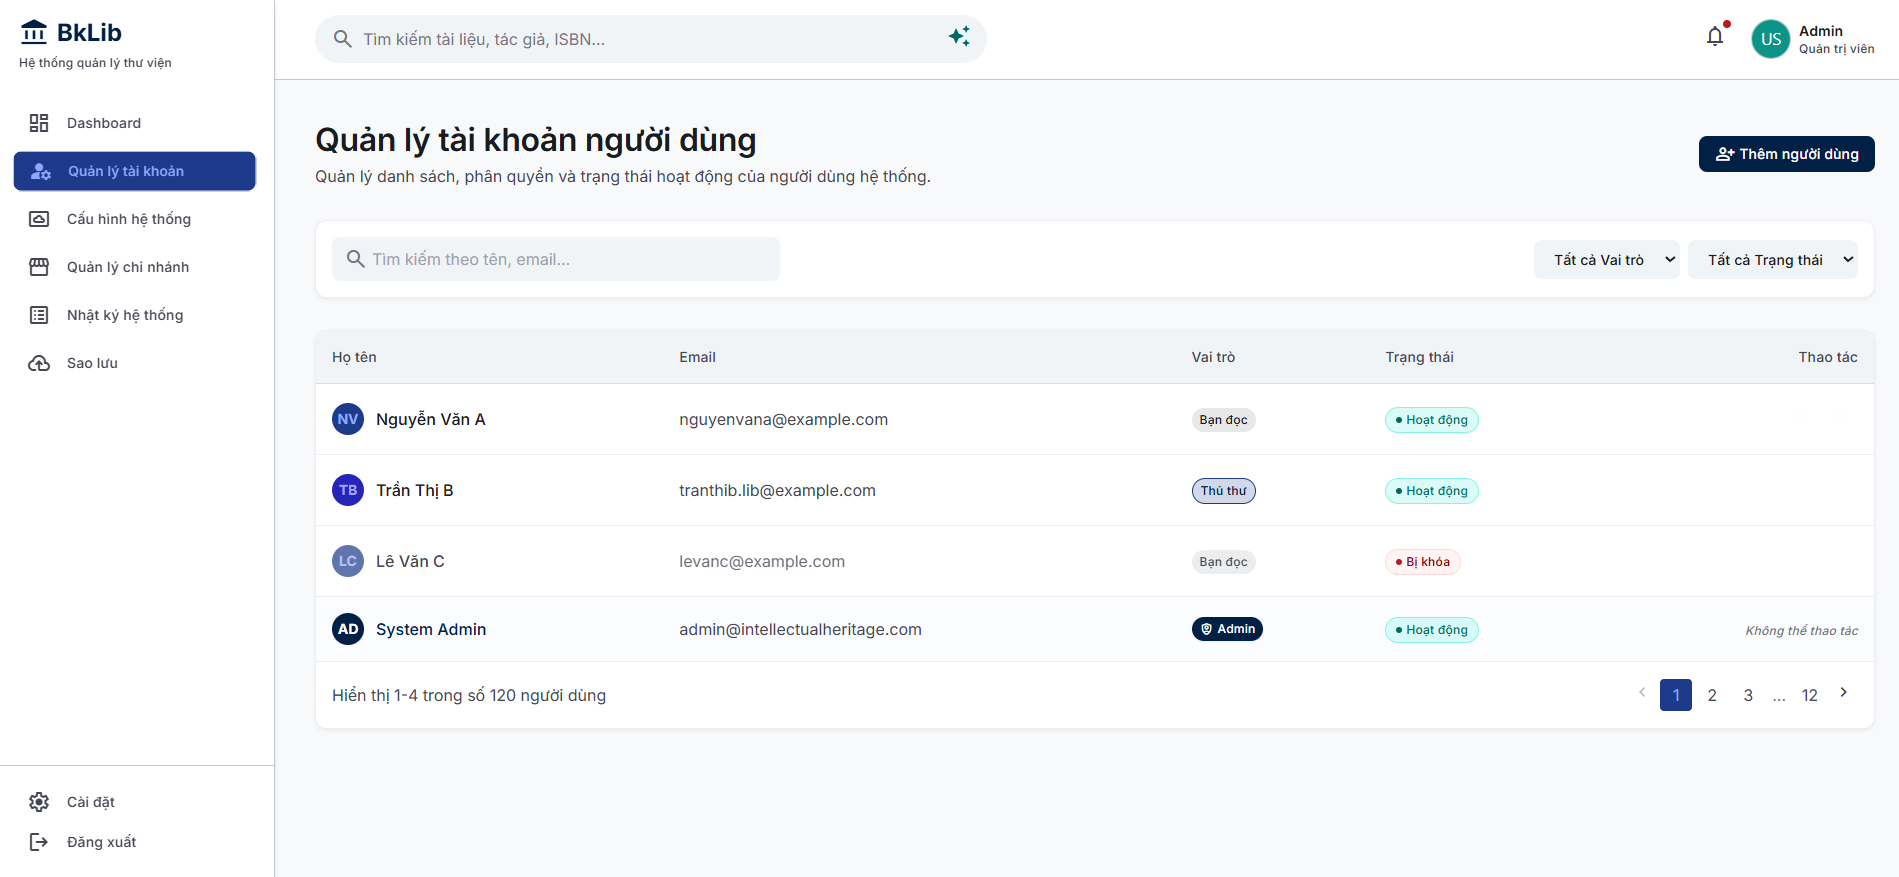
\includegraphics[width=0.95\linewidth]{Images/Admin_QuanLyTaiKhoan.png}
    \vspace{10pt}
    \caption{Giao diện Trang Quản lý tài khoản người dùng}
    \label{fig:admin_user_management}
\end{figure}

\textbf{Mô tả chức năng giao diện:} Cung cấp bảng danh sách tài khoản phân trang, tích hợp thanh tìm kiếm nhanh và bộ lọc theo vai trò, trạng thái. Hỗ trợ nút chức năng thêm mới người dùng và thực hiện các thao tác khóa hoặc mở khóa quyền truy cập.

\paragraph{c) Trang Quản lý chi nhánh}
Giao diện giám sát và cấu hình các điểm thư viện vệ tinh trong mạng lưới cơ sở vật lý của hệ thống.

\begin{figure}[H]
    \centering
    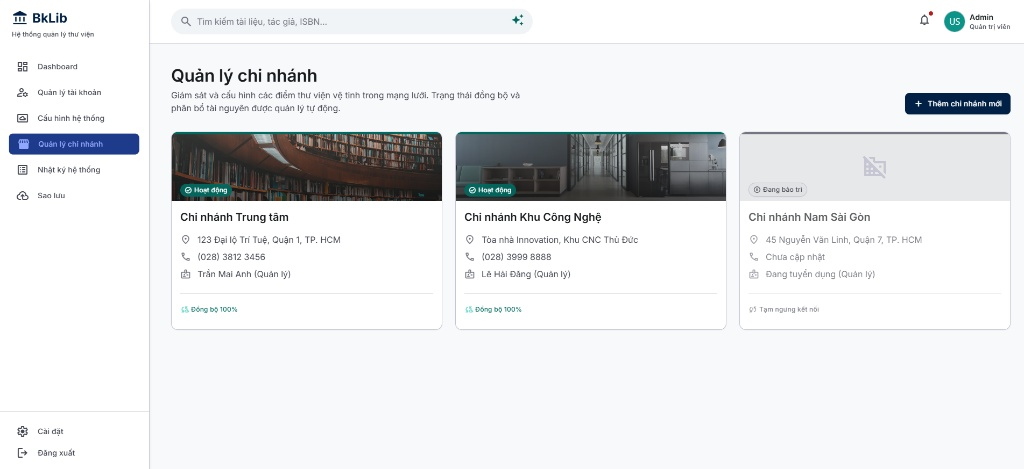
\includegraphics[width=0.95\linewidth]{Images/Admin_QuanLyChiNhanh.jpg}
    \vspace{10pt}
    \caption{Giao diện Trang Quản lý chi nhánh}
    \label{fig:admin_branch_management}
\end{figure}

\textbf{Mô tả chức năng giao diện:} Kết xuất thông tin các chi nhánh dưới dạng danh sách lưới trực quan. Mỗi thẻ chi nhánh hiển thị địa chỉ, số điện thoại hotline, tên nhân sự quản lý trực tiếp và trạng thái kết nối đồng bộ dữ liệu tài nguyên.

\paragraph{d) Trang Nhật ký kiểm toán}
Màn hình phục vụ công tác an ninh thông tin, lưu vết và phân tích toàn bộ lịch sử thao tác hệ thống của các tác nhân.

\begin{figure}[H]
    \centering
    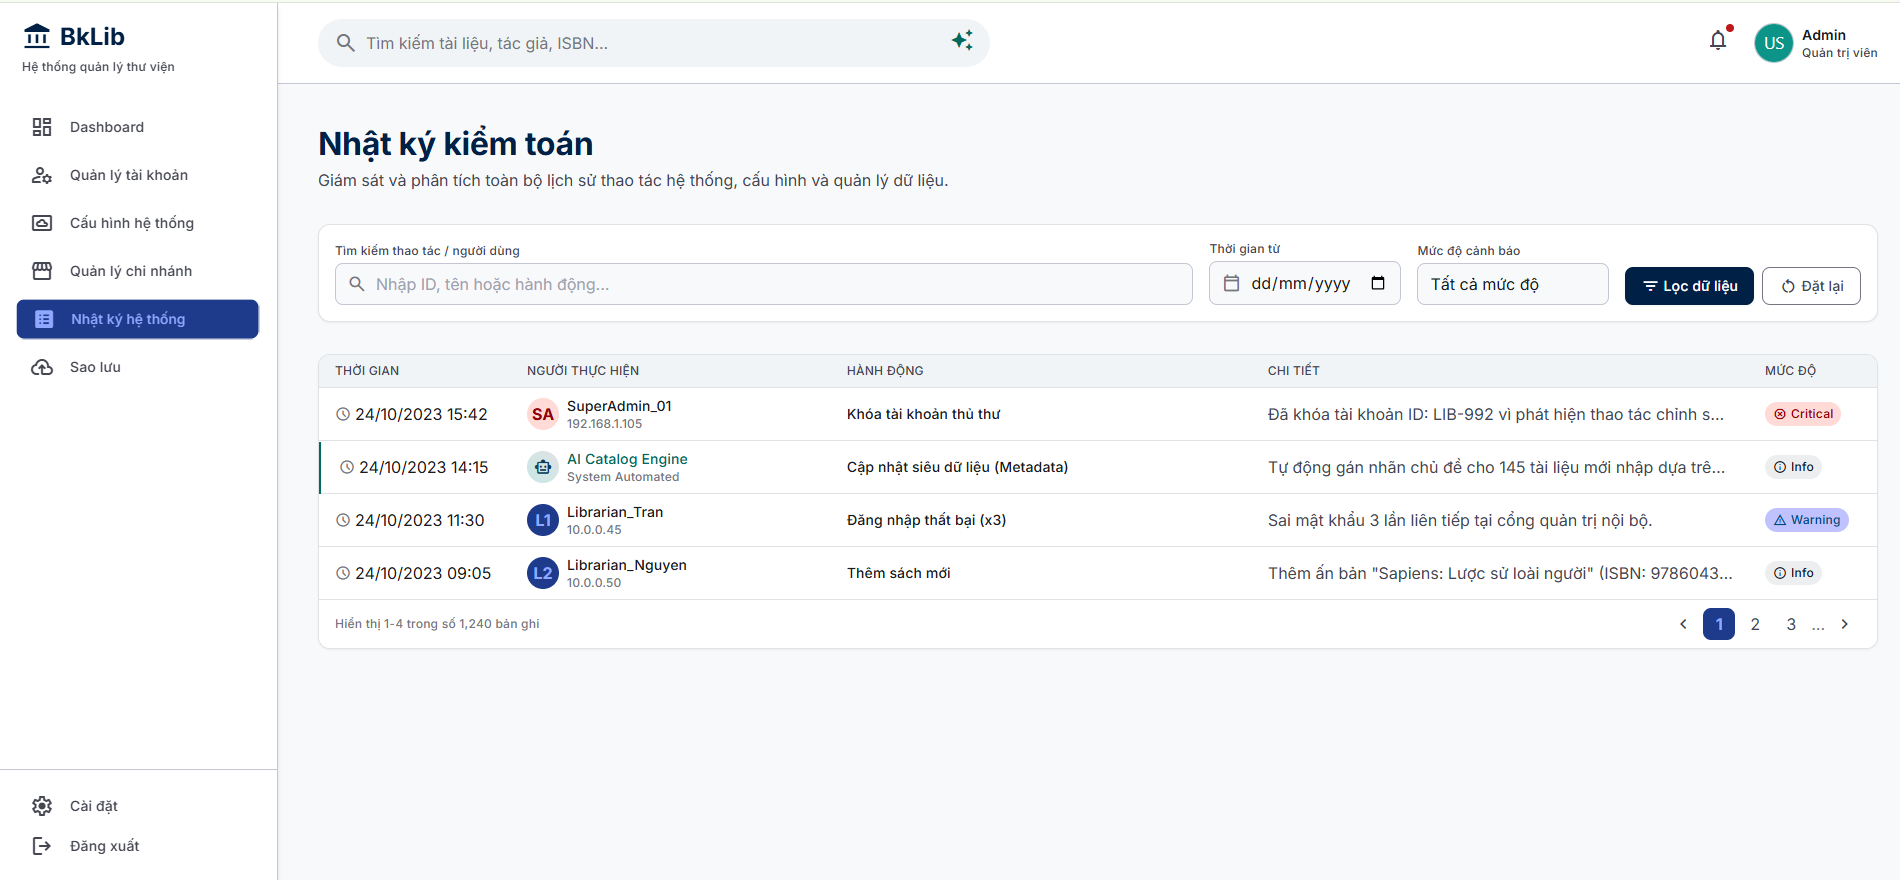
\includegraphics[width=0.95\linewidth]{Images/Admin_NhatKyKiemToan.png}
    \vspace{10pt}
    \caption{Giao diện Trang Nhật ký kiểm toán hệ thống}
    \label{fig:admin_audit_log}
\end{figure}

\textbf{Mô tả chức năng giao diện:} Bảng theo dõi phân cấp hiển thị chi tiết mốc thời gian, địa chỉ mạng IP của người thực hiện, hành động tương tác và nội dung chi tiết thay đổi cấu hình. Các dòng nhật ký được gắn nhãn phân loại mức độ rủi ro trực quan để phục vụ rà soát an ninh.

\paragraph{e) Trang Sao lưu \& Phục hồi}
Phân hệ quản trị hạ tầng cơ sở dữ liệu, đảm bảo tính toàn vẹn và an toàn thông tin trước các sự cố vận hành.

\begin{figure}[H]
    \centering
    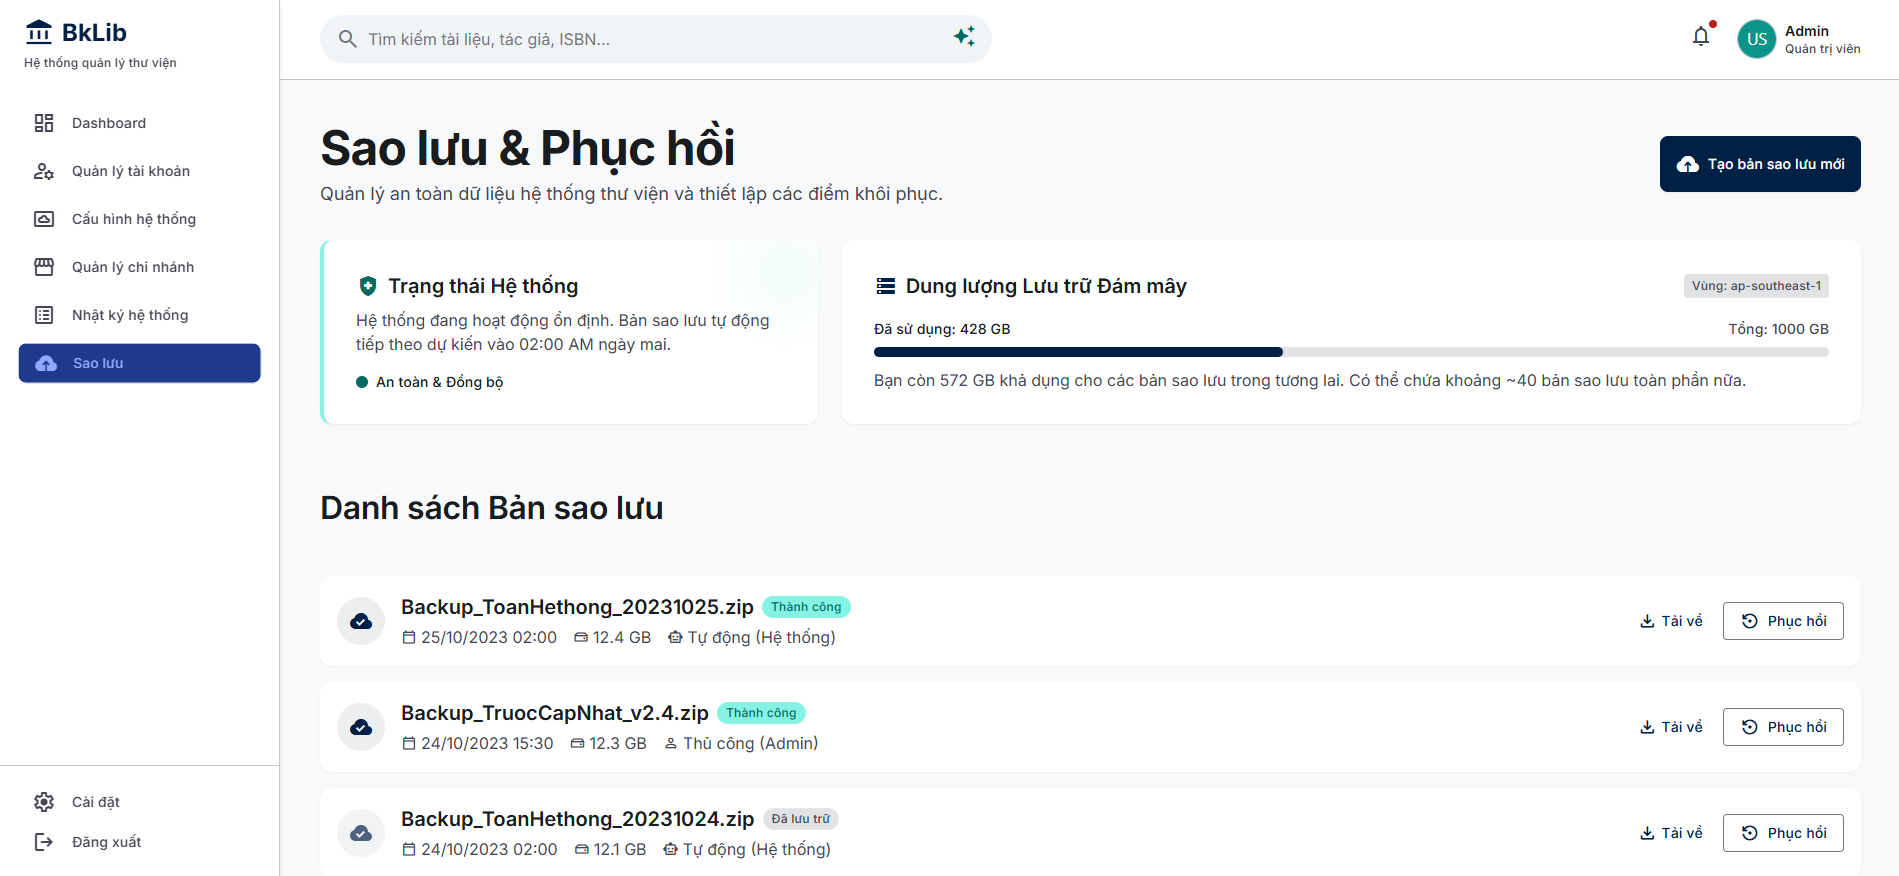
\includegraphics[width=0.95\linewidth]{Images/Admin_SaoLuuPhucHoi.png}
    \vspace{10pt}
    \caption{Giao diện Trang Sao lưu và Phục hồi dữ liệu}
    \label{fig:admin_backup}
\end{figure}

\textbf{Mô tả chức năng giao diện:} Hiển thị trạng thái đồng bộ, dung lượng vùng nhớ lưu trữ hiện hành và danh sách các bản sao lưu đã đóng gói trong quá khứ. Hỗ trợ các nút hành động tải tệp tin gốc về máy cục bộ, kích hoạt tiến trình phục hồi dữ liệu từ ảnh chụp hoặc khởi tạo bản sao lưu mới thủ công.